\documentclass{beamer}

\usetheme[bgphoto]{polimi}
% Full instructions available at:
% https://github.com/elauksap/beamerthemepolimi

% Set custom font (requires to compile with XeLaTeX).
\usepackage{ifxetex}
\ifxetex
    \usepackage{fontspec}
    \setsansfont[Scale=0.95]{Arial}
\fi

\usepackage{subfig} % Numbered and caption subfigures using \subfloat.
\usepackage[font={scriptsize}]{caption}
\usepackage{mathtools}

\usepackage{lipsum}

\title{Three-Dimensional Bin Packing \\ with Vertical Support}
\subtitle{}
\author{Jacopo Libè}
\date{952914}

\begin{document}
    \begin{frame}
        \maketitle
    \end{frame}
    
    \begin{frame}{Table of contents}
      \tableofcontents
    \end{frame}
    
    \section{Introduction}
    \begin{frame}{Case study}
        \begin{columns}[onlytextwidth,T]
            \column{\dimexpr\linewidth-55mm-5mm}
                \begin{itemize}
                    \item Large warehouses
                    \item Mixed-case palletization
                    \item No control over items' shape (strongly heterogeneous)
                    \item Pallets wrapped during loading procedure
                \end{itemize}
                \vspace{-5mm}
                \begin{figure}[H]
                    \resizebox{\columnwidth}{!}{%
                        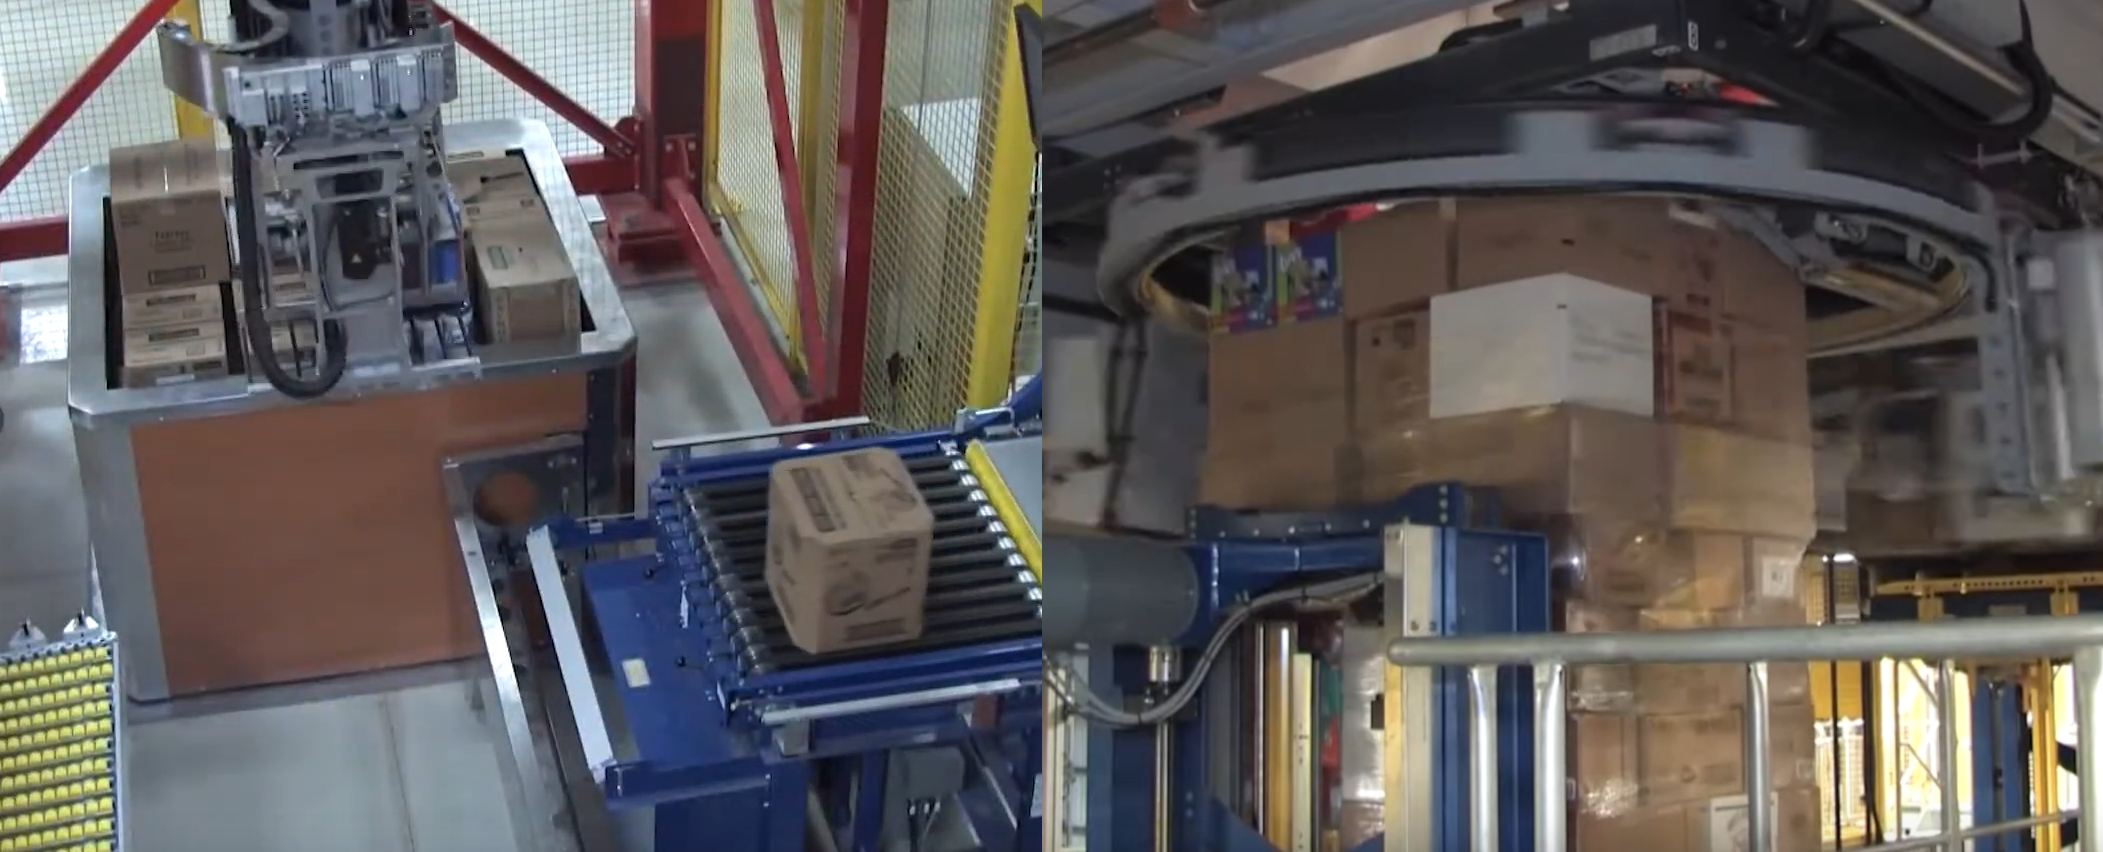
\includegraphics{Images/presentation/example_pit_pallettization.png}
                    }
                    \caption{Example of pit pallettization (\hyperlink{https://www.youtube.com/watch?v=_sSdk1baNLA}{Schäfer Case Picking | SSI SCHÄFER})}
                \end{figure}
            \column{55mm}
                \begin{figure}
                    \resizebox{\columnwidth}{!}{%
                        
\includegraphics{Images/logo_ermesx_highcontrast}
                    }
                \end{figure}
                \begin{figure}
                    \resizebox{\columnwidth}{!}{%
                        

\tikzset{every picture/.style={line width=0.75pt}} %set default line width to 0.75pt        

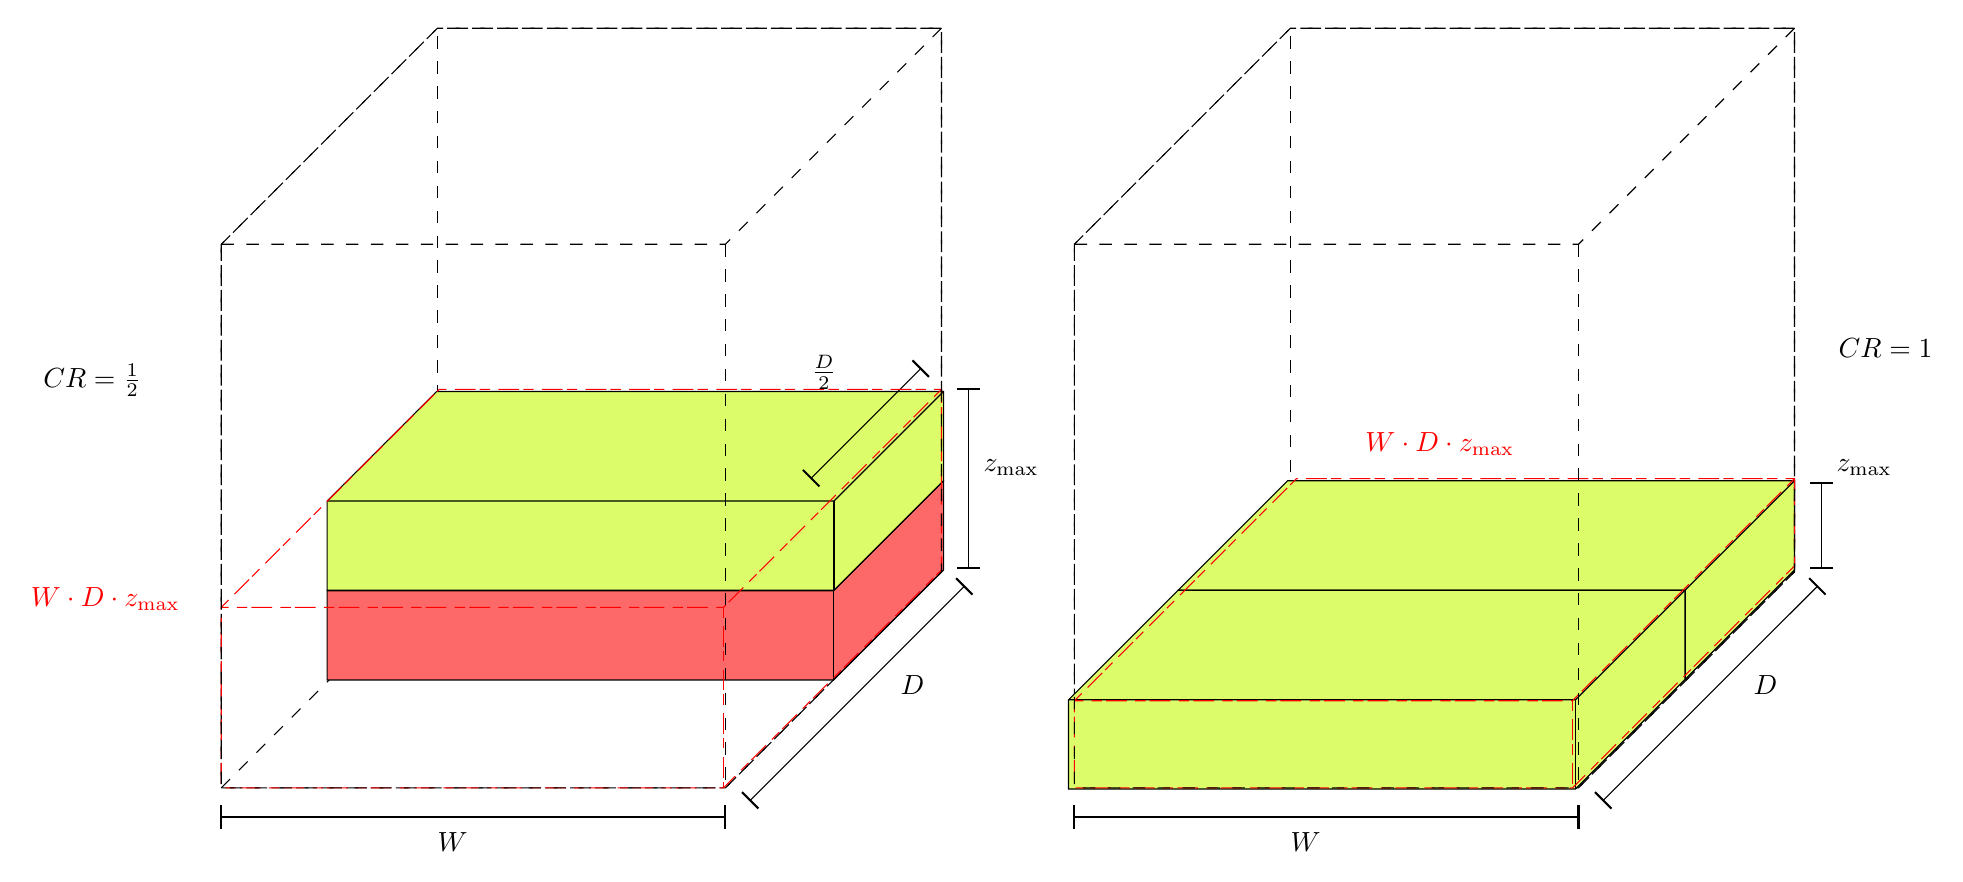
\begin{tikzpicture}[x=0.75pt,y=0.75pt,yscale=-1,xscale=1]
%uncomment if require: \path (0,479); %set diagram left start at 0, and has height of 479

%Shape: Cube [id:dp9446615397697055] 
\draw  [dash pattern={on 4.5pt off 4.5pt}] (917,301.9) -- (812.9,406) -- (570,406) -- (570,144.1) -- (674.1,40) -- (917,40) -- cycle ; \draw  [dash pattern={on 4.5pt off 4.5pt}] (570,406) -- (674.1,301.9) -- (917,301.9) ; \draw  [dash pattern={on 4.5pt off 4.5pt}] (674.1,301.9) -- (674.1,40) ;
%Shape: Cube [id:dp9924623151681093] 
\draw  [fill={rgb, 255:red, 220; green, 253; blue, 105 }  ,fill opacity=1 ] (620,310.78) -- (672.78,258) -- (917,258) -- (917,301) -- (864.22,353.78) -- (620,353.78) -- cycle ; \draw   (917,258) -- (864.22,310.78) -- (620,310.78) ; \draw   (864.22,310.78) -- (864.22,353.78) ;
%Shape: Cube [id:dp4356357707795666] 
\draw  [fill={rgb, 255:red, 220; green, 253; blue, 105 }  ,fill opacity=1 ] (567.22,363.56) -- (620,310.78) -- (864.22,310.78) -- (864.22,353.78) -- (811.44,406.56) -- (567.22,406.56) -- cycle ; \draw   (864.22,310.78) -- (811.44,363.56) -- (567.22,363.56) ; \draw   (811.44,363.56) -- (811.44,406.56) ;
%Shape: Cube [id:dp900981008021689] 
\draw  [dash pattern={on 4.5pt off 4.5pt}] (506,301.9) -- (401.9,406) -- (159,406) -- (159,144.1) -- (263.1,40) -- (506,40) -- cycle ; \draw  [dash pattern={on 4.5pt off 4.5pt}] (159,406) -- (263.1,301.9) -- (506,301.9) ; \draw  [dash pattern={on 4.5pt off 4.5pt}] (263.1,301.9) -- (263.1,40) ;
%Shape: Cube [id:dp9462720863667783] 
\draw  [fill={rgb, 255:red, 253; green, 105; blue, 105 }  ,fill opacity=1 ] (210,311) -- (263,258) -- (507,258) -- (507,301) -- (454,354) -- (210,354) -- cycle ; \draw   (507,258) -- (454,311) -- (210,311) ; \draw   (454,311) -- (454,354) ;
%Shape: Cube [id:dp20686523528460465] 
\draw  [fill={rgb, 255:red, 220; green, 253; blue, 105 }  ,fill opacity=1 ] (210,267.78) -- (262.78,215) -- (507,215) -- (507,258) -- (454.22,310.78) -- (210,310.78) -- cycle ; \draw   (507,215) -- (454.22,267.78) -- (210,267.78) ; \draw   (454.22,267.78) -- (454.22,310.78) ;
%Straight Lines [id:da9583369995131138] 
\draw    (496,204) -- (443.22,256.78) ;
\draw [shift={(443.22,256.78)}, rotate = 315] [color={rgb, 255:red, 0; green, 0; blue, 0 }  ][line width=0.75]    (0,5.59) -- (0,-5.59)   ;
\draw [shift={(496,204)}, rotate = 315] [color={rgb, 255:red, 0; green, 0; blue, 0 }  ][line width=0.75]    (0,5.59) -- (0,-5.59)   ;
%Straight Lines [id:da4480701288134522] 
\draw    (401.9,420) -- (159,420) ;
\draw [shift={(159,420)}, rotate = 360] [color={rgb, 255:red, 0; green, 0; blue, 0 }  ][line width=0.75]    (0,5.59) -- (0,-5.59)   ;
\draw [shift={(401.9,420)}, rotate = 360] [color={rgb, 255:red, 0; green, 0; blue, 0 }  ][line width=0.75]    (0,5.59) -- (0,-5.59)   ;
%Straight Lines [id:da9761873387202039] 
\draw    (517,308.9) -- (413.86,412) ;
\draw [shift={(413.86,412)}, rotate = 315.01] [color={rgb, 255:red, 0; green, 0; blue, 0 }  ][line width=0.75]    (0,5.59) -- (0,-5.59)   ;
\draw [shift={(517,308.9)}, rotate = 315.01] [color={rgb, 255:red, 0; green, 0; blue, 0 }  ][line width=0.75]    (0,5.59) -- (0,-5.59)   ;
%Straight Lines [id:da1211437330301477] 
\draw    (519,214) -- (519,299.86) ;
\draw [shift={(519,299.86)}, rotate = 270] [color={rgb, 255:red, 0; green, 0; blue, 0 }  ][line width=0.75]    (0,5.59) -- (0,-5.59)   ;
\draw [shift={(519,214)}, rotate = 270] [color={rgb, 255:red, 0; green, 0; blue, 0 }  ][line width=0.75]    (0,5.59) -- (0,-5.59)   ;
%Shape: Cube [id:dp6016430781165488] 
\draw  [color={rgb, 255:red, 255; green, 0; blue, 0 }  ,draw opacity=1 ][dash pattern={on 3.75pt off 3pt on 7.5pt off 1.5pt}] (159,319) -- (264,214) -- (506,214) -- (506,301) -- (401,406) -- (159,406) -- cycle ; \draw  [color={rgb, 255:red, 255; green, 0; blue, 0 }  ,draw opacity=1 ][dash pattern={on 3.75pt off 3pt on 7.5pt off 1.5pt}] (506,214) -- (401,319) -- (159,319) ; \draw  [color={rgb, 255:red, 255; green, 0; blue, 0 }  ,draw opacity=1 ][dash pattern={on 3.75pt off 3pt on 7.5pt off 1.5pt}] (401,319) -- (401,406) ;
%Shape: Cube [id:dp9858212525551202] 
\draw  [dash pattern={on 4.5pt off 4.5pt}] (159,144.1) -- (263.1,40) -- (506,40) -- (506,301.9) -- (401.9,406) -- (159,406) -- cycle ; \draw  [dash pattern={on 4.5pt off 4.5pt}] (506,40) -- (401.9,144.1) -- (159,144.1) ; \draw  [dash pattern={on 4.5pt off 4.5pt}] (401.9,144.1) -- (401.9,406) ;
%Straight Lines [id:da4537070040642701] 
\draw    (812.9,420) -- (570,420) ;
\draw [shift={(570,420)}, rotate = 360] [color={rgb, 255:red, 0; green, 0; blue, 0 }  ][line width=0.75]    (0,5.59) -- (0,-5.59)   ;
\draw [shift={(812.9,420)}, rotate = 360] [color={rgb, 255:red, 0; green, 0; blue, 0 }  ][line width=0.75]    (0,5.59) -- (0,-5.59)   ;
%Straight Lines [id:da13051427322471099] 
\draw    (928,308.9) -- (824.86,412) ;
\draw [shift={(824.86,412)}, rotate = 315.01] [color={rgb, 255:red, 0; green, 0; blue, 0 }  ][line width=0.75]    (0,5.59) -- (0,-5.59)   ;
\draw [shift={(928,308.9)}, rotate = 315.01] [color={rgb, 255:red, 0; green, 0; blue, 0 }  ][line width=0.75]    (0,5.59) -- (0,-5.59)   ;
%Straight Lines [id:da38828166025774113] 
\draw    (930,259) -- (930,299.86) ;
\draw [shift={(930,299.86)}, rotate = 270] [color={rgb, 255:red, 0; green, 0; blue, 0 }  ][line width=0.75]    (0,5.59) -- (0,-5.59)   ;
\draw [shift={(930,259)}, rotate = 270] [color={rgb, 255:red, 0; green, 0; blue, 0 }  ][line width=0.75]    (0,5.59) -- (0,-5.59)   ;
%Shape: Cube [id:dp33203292048167843] 
\draw  [color={rgb, 255:red, 255; green, 0; blue, 0 }  ,draw opacity=1 ][dash pattern={on 3.75pt off 3pt on 7.5pt off 1.5pt}] (570,364) -- (677,257) -- (917,257) -- (917,299) -- (810,406) -- (570,406) -- cycle ; \draw  [color={rgb, 255:red, 255; green, 0; blue, 0 }  ,draw opacity=1 ][dash pattern={on 3.75pt off 3pt on 7.5pt off 1.5pt}] (917,257) -- (810,364) -- (570,364) ; \draw  [color={rgb, 255:red, 255; green, 0; blue, 0 }  ,draw opacity=1 ][dash pattern={on 3.75pt off 3pt on 7.5pt off 1.5pt}] (810,364) -- (810,406) ;
%Shape: Cube [id:dp6959350788468752] 
\draw  [dash pattern={on 4.5pt off 4.5pt}] (570,144.1) -- (674.1,40) -- (917,40) -- (917,301.9) -- (812.9,406) -- (570,406) -- cycle ; \draw  [dash pattern={on 4.5pt off 4.5pt}] (917,40) -- (812.9,144.1) -- (570,144.1) ; \draw  [dash pattern={on 4.5pt off 4.5pt}] (812.9,144.1) -- (812.9,406) ;

% Text Node
\draw (442,196.4) node [anchor=north west][inner sep=0.75pt]    {$\frac{D}{2}$};
% Text Node
\draw (262,426.4) node [anchor=north west][inner sep=0.75pt]    {$W$};
% Text Node
\draw (485,350.4) node [anchor=north west][inner sep=0.75pt]    {$D$};
% Text Node
\draw (72,200.4) node [anchor=north west][inner sep=0.75pt]    {$CR=\frac{1}{2}$};
% Text Node
\draw (525,246.4) node [anchor=north west][inner sep=0.75pt]    {$z_{\text{max}}$};
% Text Node
\draw (66,308.4) node [anchor=north west][inner sep=0.75pt]  [color={rgb, 255:red, 255; green, 0; blue, 0 }  ,opacity=1 ]  {$W\cdot D\cdot z_{\text{max}}$};
% Text Node
\draw (673,426.4) node [anchor=north west][inner sep=0.75pt]    {$W$};
% Text Node
\draw (896,350.4) node [anchor=north west][inner sep=0.75pt]    {$D$};
% Text Node
\draw (937,188.4) node [anchor=north west][inner sep=0.75pt]    {$CR=1$};
% Text Node
\draw (936,246.4) node [anchor=north west][inner sep=0.75pt]    {$z_{\text{max}}$};
% Text Node
\draw (709,233.4) node [anchor=north west][inner sep=0.75pt]  [color={rgb, 255:red, 255; green, 0; blue, 0 }  ,opacity=1 ]  {$W\cdot D\cdot z_{\text{max}}$};


\end{tikzpicture}

                    }
                    \caption{Cage ratio of two different bin configurations}
                    \label{fig:cage_ratio}
                \end{figure}
        \end{columns}
    \end{frame}

    \begin{frame}{Vertical Support}
        \begin{block}{Definition}
            An item has vertical support if one of the following conditions hold:
            \begin{itemize}
                \item \textbf{Condition 1}: at least a percentage $\alpha_s$ of its base area is resting on other items
                \item \textbf{Condition 2}: at least 3 of its vertices are resting over other items and \textbf{Condition 1} holds with a lower percentage
            \end{itemize}
        \end{block}
    \end{frame}



    \begin{frame}{Vertical Support}
        \begin{figure}[H]
            \resizebox{\columnwidth}{!}{%
                

\tikzset{every picture/.style={line width=0.75pt}} %set default line width to 0.75pt        

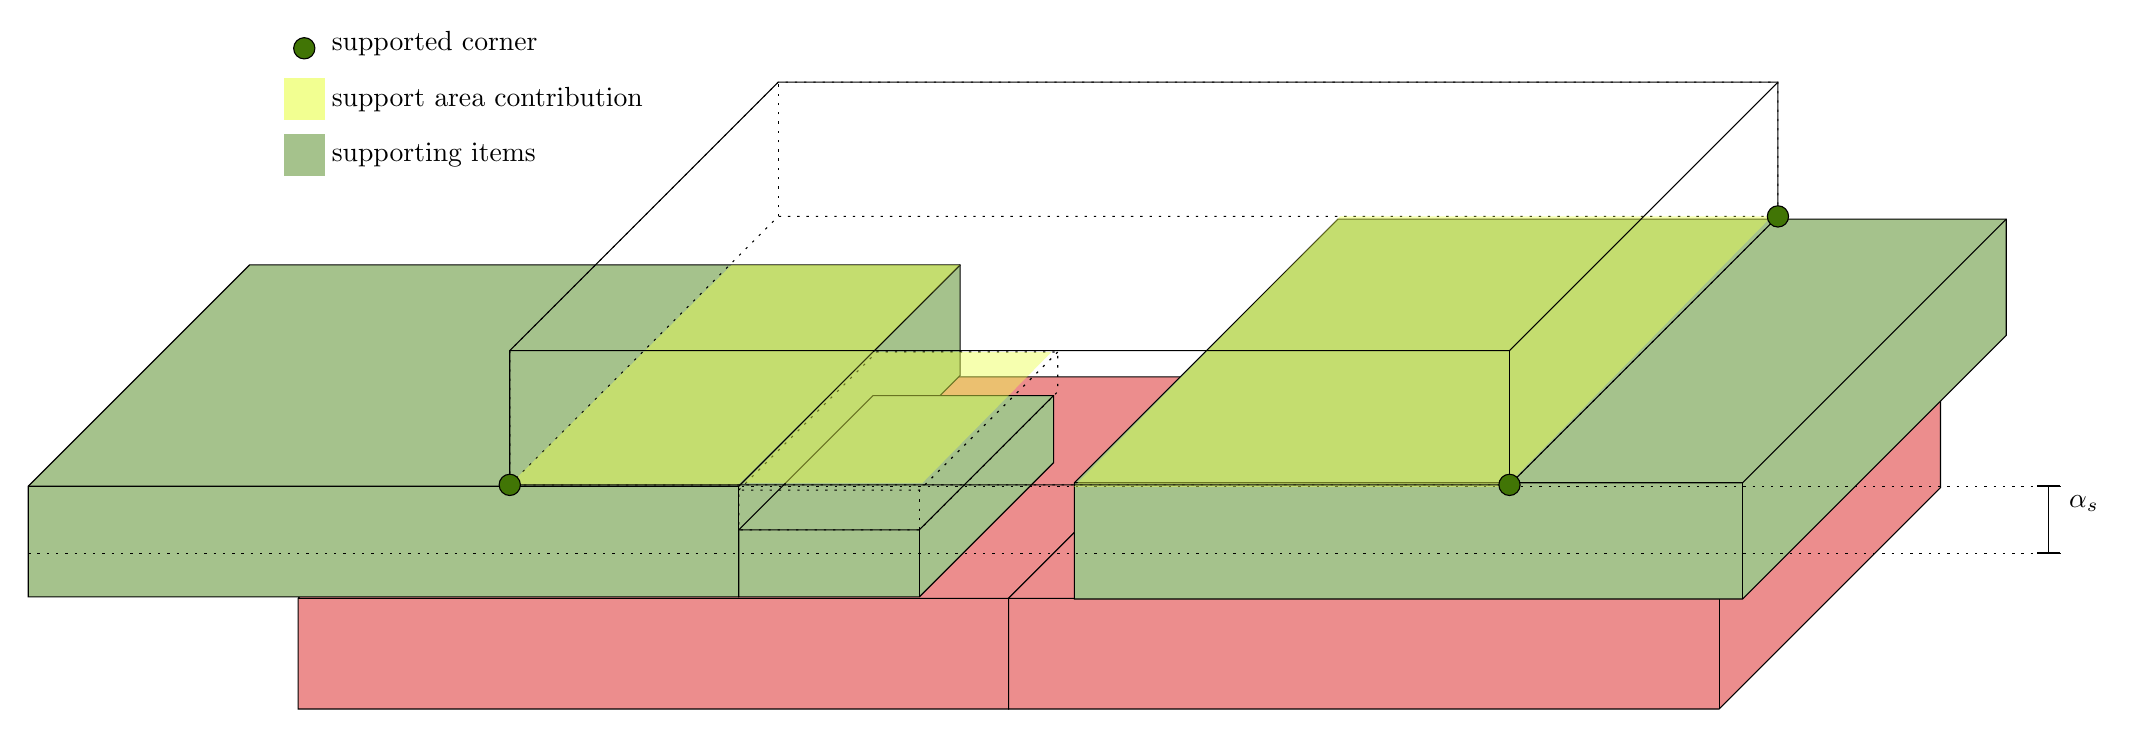
\begin{tikzpicture}[x=0.75pt,y=0.75pt,yscale=-1,xscale=1]
%uncomment if require: \path (0,479); %set diagram left start at 0, and has height of 479

%Shape: Cube [id:dp9411979483763162] 
\draw  [fill={rgb, 255:red, 236; green, 141; blue, 141 }  ,fill opacity=1 ] (194,306.67) -- (300.67,200) -- (643,200) -- (643,253.33) -- (536.33,360) -- (194,360) -- cycle ; \draw   (643,200) -- (536.33,306.67) -- (194,306.67) ; \draw   (536.33,306.67) -- (536.33,360) ;
%Shape: Cube [id:dp993645103603593] 
\draw  [fill={rgb, 255:red, 236; green, 141; blue, 141 }  ,fill opacity=1 ] (536.33,306.67) -- (643,200) -- (985.33,200) -- (985.33,253.33) -- (878.67,360) -- (536.33,360) -- cycle ; \draw   (985.33,200) -- (878.67,306.67) -- (536.33,306.67) ; \draw   (878.67,306.67) -- (878.67,360) ;
%Shape: Cube [id:dp23986673546182513] 
\draw  [fill={rgb, 255:red, 165; green, 194; blue, 140 }  ,fill opacity=1 ] (64,252.67) -- (170.67,146) -- (513,146) -- (513,199.33) -- (406.33,306) -- (64,306) -- cycle ; \draw   (513,146) -- (406.33,252.67) -- (64,252.67) ; \draw   (406.33,252.67) -- (406.33,306) ;
%Shape: Cube [id:dp5474008601617114] 
\draw  [fill={rgb, 255:red, 165; green, 194; blue, 140 }  ,fill opacity=1 ] (406.33,273.67) -- (471,209) -- (558,209) -- (558,241.33) -- (493.33,306) -- (406.33,306) -- cycle ; \draw   (558,209) -- (493.33,273.67) -- (406.33,273.67) ; \draw   (493.33,273.67) -- (493.33,306) ;
%Shape: Cube [id:dp7313777533771082] 
\draw  [fill={rgb, 255:red, 165; green, 194; blue, 140 }  ,fill opacity=1 ] (568,251) -- (695,124) -- (1017,124) -- (1017,180) -- (890,307) -- (568,307) -- cycle ; \draw   (1017,124) -- (890,251) -- (568,251) ; \draw   (890,251) -- (890,307) ;
%Shape: Cube [id:dp9978562503762016] 
\draw  [dash pattern={on 0.84pt off 2.51pt}] (907,122.67) -- (777.67,252) -- (296,252) -- (296,187.33) -- (425.33,58) -- (907,58) -- cycle ; \draw  [dash pattern={on 0.84pt off 2.51pt}] (296,252) -- (425.33,122.67) -- (907,122.67) ; \draw  [dash pattern={on 0.84pt off 2.51pt}] (425.33,122.67) -- (425.33,58) ;
%Shape: Cube [id:dp48964002783685845] 
\draw  [color={rgb, 255:red, 0; green, 0; blue, 0 }  ,draw opacity=1 ][fill={rgb, 255:red, 255; green, 255; blue, 255 }  ,fill opacity=0 ][dash pattern={on 0.84pt off 2.51pt}] (406.33,254.53) -- (472.86,188) -- (560,188) -- (560,207.14) -- (493.47,273.67) -- (406.33,273.67) -- cycle ; \draw  [color={rgb, 255:red, 0; green, 0; blue, 0 }  ,draw opacity=1 ][dash pattern={on 0.84pt off 2.51pt}] (560,188) -- (493.47,254.53) -- (406.33,254.53) ; \draw  [color={rgb, 255:red, 0; green, 0; blue, 0 }  ,draw opacity=1 ][dash pattern={on 0.84pt off 2.51pt}] (493.47,254.53) -- (493.47,273.67) ;
%Straight Lines [id:da26590658600836115] 
\draw    (1037.33,252.67) -- (1037.33,285) ;
\draw [shift={(1037.33,285)}, rotate = 270] [color={rgb, 255:red, 0; green, 0; blue, 0 }  ][line width=0.75]    (0,5.59) -- (0,-5.59)   ;
\draw [shift={(1037.33,252.67)}, rotate = 270] [color={rgb, 255:red, 0; green, 0; blue, 0 }  ][line width=0.75]    (0,5.59) -- (0,-5.59)   ;
%Straight Lines [id:da8302030012021052] 
\draw  [dash pattern={on 0.84pt off 2.51pt}]  (64,285) -- (1044,285) ;
%Straight Lines [id:da5354149137938202] 
\draw  [dash pattern={on 0.84pt off 2.51pt}]  (64,252.67) -- (1044,252.67) ;
%Shape: Parallelogram [id:dp4597753988697182] 
\draw  [color={rgb, 255:red, 0; green, 0; blue, 0 }  ,draw opacity=0 ][fill={rgb, 255:red, 234; green, 255; blue, 77 }  ,fill opacity=0.45 ] (403,146) -- (513,146) -- (406,252) -- (296,252) -- cycle ;
%Shape: Parallelogram [id:dp9407100355043312] 
\draw  [color={rgb, 255:red, 0; green, 0; blue, 0 }  ,draw opacity=0 ][fill={rgb, 255:red, 234; green, 255; blue, 77 }  ,fill opacity=0.45 ] (471,188) -- (557,188) -- (494.86,251) -- (408.86,251) -- cycle ;
%Shape: Parallelogram [id:dp5499917231467685] 
\draw  [color={rgb, 255:red, 0; green, 0; blue, 0 }  ,draw opacity=0 ][fill={rgb, 255:red, 234; green, 255; blue, 77 }  ,fill opacity=0.45 ] (696,122.67) -- (904,122.67) -- (775.67,253) -- (567.67,253) -- cycle ;
%Shape: Cube [id:dp21506487392572304] 
\draw   (296,187.33) -- (425.33,58) -- (907,58) -- (907,122.67) -- (777.67,252) -- (296,252) -- cycle ; \draw   (907,58) -- (777.67,187.33) -- (296,187.33) ; \draw   (777.67,187.33) -- (777.67,252) ;
%Shape: Rectangle [id:dp8515603217170198] 
\draw  [color={rgb, 255:red, 0; green, 0; blue, 0 }  ,draw opacity=0 ][fill={rgb, 255:red, 234; green, 255; blue, 77 }  ,fill opacity=0.62 ] (187,56) -- (207,56) -- (207,76) -- (187,76) -- cycle ;
%Shape: Rectangle [id:dp8969674268045522] 
\draw  [color={rgb, 255:red, 0; green, 0; blue, 0 }  ,draw opacity=0 ][fill={rgb, 255:red, 165; green, 194; blue, 140 }  ,fill opacity=1 ] (187,83) -- (207,83) -- (207,103) -- (187,103) -- cycle ;
%Shape: Circle [id:dp08410160878408413] 
\draw  [fill={rgb, 255:red, 65; green, 117; blue, 5 }  ,fill opacity=1 ] (290.88,252) .. controls (290.88,249.17) and (293.17,246.88) .. (296,246.88) .. controls (298.83,246.88) and (301.13,249.17) .. (301.13,252) .. controls (301.13,254.83) and (298.83,257.13) .. (296,257.13) .. controls (293.17,257.13) and (290.88,254.83) .. (290.88,252) -- cycle ;
%Shape: Circle [id:dp20799682119759832] 
\draw  [fill={rgb, 255:red, 65; green, 117; blue, 5 }  ,fill opacity=1 ] (772.54,252) .. controls (772.54,249.17) and (774.84,246.88) .. (777.67,246.88) .. controls (780.5,246.88) and (782.79,249.17) .. (782.79,252) .. controls (782.79,254.83) and (780.5,257.13) .. (777.67,257.13) .. controls (774.84,257.13) and (772.54,254.83) .. (772.54,252) -- cycle ;
%Shape: Circle [id:dp9242580914559287] 
\draw  [fill={rgb, 255:red, 65; green, 117; blue, 5 }  ,fill opacity=1 ] (901.88,122.67) .. controls (901.88,119.84) and (904.17,117.54) .. (907,117.54) .. controls (909.83,117.54) and (912.13,119.84) .. (912.13,122.67) .. controls (912.13,125.5) and (909.83,127.79) .. (907,127.79) .. controls (904.17,127.79) and (901.88,125.5) .. (901.88,122.67) -- cycle ;
%Shape: Circle [id:dp40386474009325335] 
\draw  [fill={rgb, 255:red, 65; green, 117; blue, 5 }  ,fill opacity=1 ] (191.88,41.67) .. controls (191.88,38.84) and (194.17,36.54) .. (197,36.54) .. controls (199.83,36.54) and (202.13,38.84) .. (202.13,41.67) .. controls (202.13,44.5) and (199.83,46.79) .. (197,46.79) .. controls (194.17,46.79) and (191.88,44.5) .. (191.88,41.67) -- cycle ;

% Text Node
\draw (1046,256.07) node [anchor=north west][inner sep=0.75pt]    {$\alpha _{s}$};
% Text Node
\draw (209,59) node [anchor=north west][inner sep=0.75pt]   [align=left] {support area contribution};
% Text Node
\draw (209,86) node [anchor=north west][inner sep=0.75pt]   [align=left] {supporting items};
% Text Node
\draw (209,32) node [anchor=north west][inner sep=0.75pt]   [align=left] {supported corner};


\end{tikzpicture}

            }
            \caption{Representation of an item with conditions 1 and 2 of vertical support given $\alpha_s = 0.5, \beta_s$}
            \label{fig:support}
        \end{figure}
    \end{frame}

    \section{Problem Definition}
    \begin{frame}{Literature Review}
        %TODO: Images for placement strategies
        \begin{itemize}
            \item The problem is NP-Hard
            \item Exact methods only for small instances %Cite?
            \item Existing 3D-BPP heuristics don't consider practical constraints
            \item Solutions for container loading and pallet loading problems are layer based
        \end{itemize}
    \end{frame}

    \begin{frame}{Conceptual Formulation}
        \begin{eqnarray*}
            \textbf{minimize} & \text{number of used bins} \\
            \textbf{then, maximize} & \text{average cage ratio of the used bins} \\
            \textbf{subject to} & \text{all items are assigned to one and only one bin} \\
                                              & \text{all items are inside the bin's bounds} \\
                                              & \text{no overlaps between items in the same bin} \\
                                              & \text{all items have vertical support} \\
        \end{eqnarray*}
    \end{frame}

    \begin{frame}{MILP Proxy Model - Objective Function}

        \begin{columns}[onlytextwidth,T]
            \column{\dimexpr\linewidth-75mm-5mm}
                \vspace{.25\textheight}
                \hspace{-5mm}
                \resizebox{17mm}{!}{
                    \begin{minipage}{\linewidth}
                    \begin{eqnarray*}
                        \textbf{minimize} & \text{number of used bins} \\
                        \textbf{then, maximize} & \text{average cage ratio of the used bins} \\
                        \color{gray}
                        \textbf{subject to} & \color{gray} \text{all items are assigned to one and only one bin} \\
                                                            & \color{gray} \text{all items are inside the bin's bounds} \\
                                                            & \color{gray} \text{no overlaps between items in the same bin} \\
                                                            & \color{gray} \text{all items have vertical support} \\
                    \end{eqnarray*}
                    \end{minipage}
                }

            \column{75mm}
            \resizebox{!}{30mm}{
                \begin{minipage}{\linewidth}
                    \begin{align}
                       \min       \qquad& \sum\limits_{b \in B} (H v_b + z^{max}_b) & \notag \\
                      \text{s.t.} \qquad & \color{gray} \sum\limits_{b \in B} u_{ib} + \sum\limits_{b \in B} u_{jb} = 1                          & \color{gray} \forall (i, j) \in I^{OR} \notag \\
                                         & \color{gray} u_{ib} \le v_b                                                                           & \color{gray} \forall i \in I, \forall b \in B \notag \\
                                         & \color{gray} v_b \ge v_c                                                                              & \color{gray} \forall (b,c) \in B : b < c  \notag \\
                                         & \color{gray} x_i + w_i \le W                                                                          & \color{gray} \forall i \in I \notag \\ 
                                         & \color{gray} y_i + d_i \le D                                                                          & \color{gray} \forall i \in I \notag \\ 
                                         & \color{gray} z_i + h_i \le H                                                                          & \color{gray} \forall i \in I \notag \\ 
                                         & \color{gray} (x_i + w_i) - x_j\le W(1 - x^p_{ij})                                                     & \color{gray} \forall i,j \in I \notag \\
                                         & \color{gray} x_j - (x_i + w_i) + 1 \le W x^p_{ij}                                                     & \color{gray} \forall i,j \in I \notag \\
                                         & \color{gray} (y_i + d_i) - y_j \le D(1 - y^p_{ij})                                                    & \color{gray} \forall i,j \in I \notag \\
                                         & \color{gray} y_j - (y_i + d_i) + 1 \le D y^p_{ij}                                                     & \color{gray} \forall i,j \in I \notag \\
                                         & \color{gray} (z_i + h_i) - z_j\le H(1 - z^p_{ij})                                                     & \color{gray} \forall i,j \in I \notag \\
                                         & \color{gray} z_j - (z_i + h_i) + 1 \le H z^p_{ij}                                                     & \color{gray} \forall i,j \in I \notag \\
                                         & \color{gray} x^p_{ij} + x^p_{ji} + y^p_{ij} + y^p_{ji} + z^p_{ij} + z^p_{ji} \ge u_{ib} + u_{jb} - 1  & \color{gray} \forall i,j \in I, \forall b \in B \notag \\
                                         & z^{max}_b \ge (z_i + h_i) - H(1-u_{ib})                                                               & \forall i \in I, \forall b \in B \notag
                    \end{align}
                \end{minipage}
            }
            \end{columns}
    \end{frame}

    \begin{frame}{MILP Proxy Model - Geometric Constraints 1}

        \begin{columns}[onlytextwidth,T]
            \column{\dimexpr\linewidth-75mm-5mm}
                \vspace{.25\textheight}
                \hspace{-5mm}
                \resizebox{17mm}{!}{
                    \begin{minipage}{\linewidth}
                    \begin{eqnarray*}
                        \color{gray} \textbf{minimize} & \color{gray} \text{number of used bins} \\
                        \color{gray} \textbf{then, maximize} & \color{gray} \text{average cage ratio of the used bins} \\
                        \textbf{subject to} & \text{all items are assigned to one and only one bin} \\
                                                            & \color{gray} \text{all items are inside the bin's bounds} \\
                                                            & \color{gray} \text{no overlaps between items in the same bin} \\
                                                            & \color{gray} \text{all items have vertical support} \\
                    \end{eqnarray*}
                    \end{minipage}
                }

            \column{75mm}
            \resizebox{!}{30mm}{
                \begin{minipage}{\linewidth}
                    \begin{align}
                \color{gray} \min \qquad & \color{gray} \sum\limits_{b \in B} (H v_b + z^{max}_b)                                                & \notag \\
                      \text{s.t.} \qquad & \sum\limits_{b \in B} u_{ib} + \sum\limits_{b \in B} u_{jb} = 1                          & \forall (i, j) \in I^{OR} \notag \\
                                         & u_{ib} \le v_b                                                                           & \forall i \in I, \forall b \in B \notag \\
                                         & v_b \ge v_c                                                                              & \forall (b,c) \in B : b < c  \notag \\
                                         & \color{gray} x_i + w_i \le W                                                                          & \color{gray} \forall i \in I \notag \\ 
                                         & \color{gray} y_i + d_i \le D                                                                          & \color{gray} \forall i \in I \notag \\ 
                                         & \color{gray} z_i + h_i \le H                                                                          & \color{gray} \forall i \in I \notag \\ 
                                         & \color{gray} (x_i + w_i) - x_j\le W(1 - x^p_{ij})                                                     & \color{gray} \forall i,j \in I \notag \\
                                         & \color{gray} x_j - (x_i + w_i) + 1 \le W x^p_{ij}                                                     & \color{gray} \forall i,j \in I \notag \\
                                         & \color{gray} (y_i + d_i) - y_j \le D(1 - y^p_{ij})                                                    & \color{gray} \forall i,j \in I \notag \\
                                         & \color{gray} y_j - (y_i + d_i) + 1 \le D y^p_{ij}                                                     & \color{gray} \forall i,j \in I \notag \\
                                         & \color{gray} (z_i + h_i) - z_j\le H(1 - z^p_{ij})                                                     & \color{gray} \forall i,j \in I \notag \\
                                         & \color{gray} z_j - (z_i + h_i) + 1 \le H z^p_{ij}                                                     & \color{gray} \forall i,j \in I \notag \\
                                         & \color{gray} x^p_{ij} + x^p_{ji} + y^p_{ij} + y^p_{ji} + z^p_{ij} + z^p_{ji} \ge u_{ib} + u_{jb} - 1  & \color{gray} \forall i,j \in I, \forall b \in B \notag \\
                                         & \color{gray} z^{max}_b \ge (z_i + h_i) - H(1-u_{ib})                                                  & \color{gray} \forall i \in I, \forall b \in B \notag
                    \end{align}
                \end{minipage}
            }
            \end{columns}
    \end{frame}


    \begin{frame}{MILP Proxy Model - Geometric Constraints 2}

        \begin{columns}[onlytextwidth,T]
            \column{\dimexpr\linewidth-75mm-5mm}
                \vspace{.25\textheight}
                \hspace{-5mm}
                \resizebox{17mm}{!}{
                    \begin{minipage}{\linewidth}
                    \begin{eqnarray*}
                        \color{gray} \textbf{minimize} & \color{gray} \text{number of used bins} \\
                        \color{gray} \textbf{then, maximize} & \color{gray} \text{average cage ratio of the used bins} \\
                        \textbf{subject to} & \color{gray} \text{all items are assigned to one and only one bin} \\
                                                            & \text{all items are inside the bin's bounds} \\
                                                            & \color{gray} \text{no overlaps between items in the same bin} \\
                                                            & \color{gray} \text{all items have vertical support} \\
                    \end{eqnarray*}
                    \end{minipage}
                }

            \column{75mm}
            \resizebox{!}{30mm}{
                \begin{minipage}{\linewidth}
                    \begin{align}
                \color{gray} \min \qquad & \color{gray} \sum\limits_{b \in B} (H v_b + z^{max}_b)                                                & \notag \\
                      \text{s.t.} \qquad & \color{gray} \sum\limits_{b \in B} u_{ib} + \sum\limits_{b \in B} u_{jb} = 1                          & \color{gray} \forall (i, j) \in I^{OR} \notag \\
                                         & \color{gray} u_{ib} \le v_b                                                                           & \color{gray} \forall i \in I, \forall b \in B \notag \\
                                         & \color{gray} v_b \ge v_c                                                                              & \color{gray} \forall (b,c) \in B : b < c  \notag \\
                                         & x_i + w_i \le W                                                                          & \forall i \in I \notag \\ 
                                         & y_i + d_i \le D                                                                          & \forall i \in I \notag \\ 
                                         & z_i + h_i \le H                                                                          & \forall i \in I \notag \\ 
                                         & \color{gray} (x_i + w_i) - x_j\le W(1 - x^p_{ij})                                                     & \color{gray} \forall i,j \in I \notag \\
                                         & \color{gray} x_j - (x_i + w_i) + 1 \le W x^p_{ij}                                                     & \color{gray} \forall i,j \in I \notag \\
                                         & \color{gray} (y_i + d_i) - y_j \le D(1 - y^p_{ij})                                                    & \color{gray} \forall i,j \in I \notag \\
                                         & \color{gray} y_j - (y_i + d_i) + 1 \le D y^p_{ij}                                                     & \color{gray} \forall i,j \in I \notag \\
                                         & \color{gray} (z_i + h_i) - z_j\le H(1 - z^p_{ij})                                                     & \color{gray} \forall i,j \in I \notag \\
                                         & \color{gray} z_j - (z_i + h_i) + 1 \le H z^p_{ij}                                                     & \color{gray} \forall i,j \in I \notag \\
                                         & \color{gray} x^p_{ij} + x^p_{ji} + y^p_{ij} + y^p_{ji} + z^p_{ij} + z^p_{ji} \ge u_{ib} + u_{jb} - 1  & \color{gray} \forall i,j \in I, \forall b \in B \notag \\
                                         & \color{gray} z^{max}_b \ge (z_i + h_i) - H(1-u_{ib})                                                  & \color{gray} \forall i \in I, \forall b \in B \notag
                    \end{align}
                \end{minipage}
            }
            \end{columns}
    \end{frame}


    \begin{frame}{MILP Proxy Model - Geometric Constraints 3}

        \begin{columns}[onlytextwidth,T]
            \column{\dimexpr\linewidth-75mm-5mm}
                \vspace{.12\textheight}
                \hspace{-5mm}
                \resizebox{17mm}{!}{
                    \begin{minipage}{\linewidth}
                    \begin{eqnarray*}
                        \color{gray} \textbf{minimize} & \color{gray} \text{number of used bins} \\
                        \color{gray} \textbf{then, maximize} & \color{gray} \text{average cage ratio of the used bins} \\
                        \textbf{subject to} & \color{gray} \text{all items are assigned to one and only one bin} \\
                                                            & \color{gray} \text{all items are inside the bin's bounds} \\
                                                            & \text{no overlaps between items in the same bin} \\
                                                            & \color{gray} \text{all items have vertical support} \\
                    \end{eqnarray*}
                    \end{minipage}
                }
                
                \begin{figure}
                    \resizebox{1.35\columnwidth}{!}{
                        

\tikzset{every picture/.style={line width=0.75pt}} %set default line width to 0.75pt        

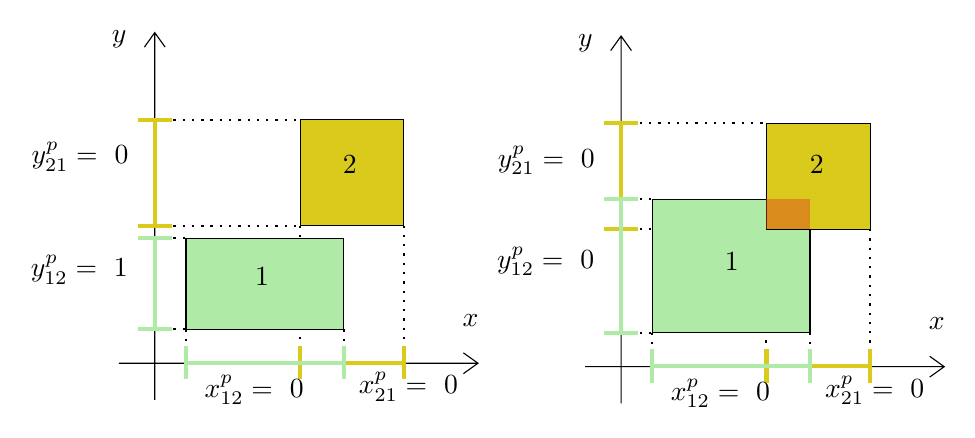
\begin{tikzpicture}[x=0.75pt,y=0.75pt,yscale=-1,xscale=1]
%uncomment if require: \path (0,300); %set diagram left start at 0, and has height of 300

%Straight Lines [id:da16944613342131554] 
\draw [color={rgb, 255:red, 0; green, 0; blue, 0 }  ,draw opacity=1 ][line width=0.75]  [dash pattern={on 0.84pt off 2.51pt}]  (77,247.5) -- (77,263.5) ;
%Straight Lines [id:da32247408153225543] 
\draw [color={rgb, 255:red, 0; green, 0; blue, 0 }  ,draw opacity=1 ][line width=0.75]  [dash pattern={on 0.84pt off 2.51pt}]  (153,247.5) -- (153,263.5) ;
%Straight Lines [id:da39889490826632257] 
\draw [color={rgb, 255:red, 0; green, 0; blue, 0 }  ,draw opacity=1 ][line width=0.75]  [dash pattern={on 0.84pt off 2.51pt}]  (182,197.5) -- (182,263.5) ;
%Straight Lines [id:da7240587122118071] 
\draw [color={rgb, 255:red, 0; green, 0; blue, 0 }  ,draw opacity=1 ][line width=0.75]  [dash pattern={on 0.84pt off 2.51pt}]  (132,197.5) -- (132,263.5) ;
%Straight Lines [id:da4848715482257471] 
\draw [color={rgb, 255:red, 0; green, 0; blue, 0 }  ,draw opacity=1 ][line width=0.75]  [dash pattern={on 0.84pt off 2.51pt}]  (62,247.5) -- (77,247.5) ;
%Straight Lines [id:da4670272012004465] 
\draw [color={rgb, 255:red, 0; green, 0; blue, 0 }  ,draw opacity=1 ][line width=0.75]  [dash pattern={on 0.84pt off 2.51pt}]  (62,203.5) -- (77,203.5) ;
%Straight Lines [id:da7178245871900936] 
\draw [color={rgb, 255:red, 0; green, 0; blue, 0 }  ,draw opacity=1 ][line width=0.75]  [dash pattern={on 0.84pt off 2.51pt}]  (62,197.5) -- (132,197.5) ;
%Straight Lines [id:da3847931225791108] 
\draw [color={rgb, 255:red, 0; green, 0; blue, 0 }  ,draw opacity=1 ][line width=0.75]  [dash pattern={on 0.84pt off 2.51pt}]  (62,146.5) -- (132,146.5) ;
%Shape: Rectangle [id:dp49230539255936656] 
\draw  [fill={rgb, 255:red, 175; green, 235; blue, 167 }  ,fill opacity=1 ] (77,203.5) -- (153,203.5) -- (153,247.5) -- (77,247.5) -- cycle ;
%Shape: Axis 2D [id:dp7101905015075989] 
\draw  (44.67,263.8) -- (217.67,263.8)(61.97,104.5) -- (61.97,281.5) (210.67,258.8) -- (217.67,263.8) -- (210.67,268.8) (56.97,111.5) -- (61.97,104.5) -- (66.97,111.5)  ;
%Shape: Rectangle [id:dp7631610956479798] 
\draw  [fill={rgb, 255:red, 217; green, 202; blue, 28 }  ,fill opacity=1 ] (132,146.5) -- (182,146.5) -- (182,197.5) -- (132,197.5) -- cycle ;
%Straight Lines [id:da5582007065184471] 
\draw [color={rgb, 255:red, 217; green, 202; blue, 28 }  ,draw opacity=1 ][line width=1.5]    (62,146.5) -- (62,197.5) ;
\draw [shift={(62,197.5)}, rotate = 270] [color={rgb, 255:red, 217; green, 202; blue, 28 }  ,draw opacity=1 ][line width=1.5]    (0,8.05) -- (0,-8.05)   ;
\draw [shift={(62,146.5)}, rotate = 270] [color={rgb, 255:red, 217; green, 202; blue, 28 }  ,draw opacity=1 ][line width=1.5]    (0,8.05) -- (0,-8.05)   ;
%Straight Lines [id:da4131577420929736] 
\draw [color={rgb, 255:red, 175; green, 235; blue, 167 }  ,draw opacity=1 ][line width=1.5]    (62,203.5) -- (62,247.5) ;
\draw [shift={(62,247.5)}, rotate = 270] [color={rgb, 255:red, 175; green, 235; blue, 167 }  ,draw opacity=1 ][line width=1.5]    (0,8.05) -- (0,-8.05)   ;
\draw [shift={(62,203.5)}, rotate = 270] [color={rgb, 255:red, 175; green, 235; blue, 167 }  ,draw opacity=1 ][line width=1.5]    (0,8.05) -- (0,-8.05)   ;
%Straight Lines [id:da9955798074260177] 
\draw [color={rgb, 255:red, 217; green, 202; blue, 28 }  ,draw opacity=1 ][line width=1.5]    (182,263.5) -- (132,263.5) ;
\draw [shift={(132,263.5)}, rotate = 360] [color={rgb, 255:red, 217; green, 202; blue, 28 }  ,draw opacity=1 ][line width=1.5]    (0,8.05) -- (0,-8.05)   ;
\draw [shift={(182,263.5)}, rotate = 360] [color={rgb, 255:red, 217; green, 202; blue, 28 }  ,draw opacity=1 ][line width=1.5]    (0,8.05) -- (0,-8.05)   ;
%Straight Lines [id:da8846703181763751] 
\draw [color={rgb, 255:red, 175; green, 235; blue, 167 }  ,draw opacity=1 ][line width=1.5]    (153,263.5) -- (77,263.5) ;
\draw [shift={(77,263.5)}, rotate = 360] [color={rgb, 255:red, 175; green, 235; blue, 167 }  ,draw opacity=1 ][line width=1.5]    (0,8.05) -- (0,-8.05)   ;
\draw [shift={(153,263.5)}, rotate = 360] [color={rgb, 255:red, 175; green, 235; blue, 167 }  ,draw opacity=1 ][line width=1.5]    (0,8.05) -- (0,-8.05)   ;
%Straight Lines [id:da49719565576066305] 
\draw [color={rgb, 255:red, 0; green, 0; blue, 0 }  ,draw opacity=1 ][line width=0.75]  [dash pattern={on 0.84pt off 2.51pt}]  (301.67,249.17) -- (301.67,265.17) ;
%Straight Lines [id:da9307804167194788] 
\draw [color={rgb, 255:red, 0; green, 0; blue, 0 }  ,draw opacity=1 ][line width=0.75]  [dash pattern={on 0.84pt off 2.51pt}]  (377.67,249.17) -- (377.67,265.17) ;
%Straight Lines [id:da8413555856997723] 
\draw [color={rgb, 255:red, 0; green, 0; blue, 0 }  ,draw opacity=1 ][line width=0.75]  [dash pattern={on 0.84pt off 2.51pt}]  (406.67,199.17) -- (406.67,265.17) ;
%Straight Lines [id:da10291713605161046] 
\draw [color={rgb, 255:red, 0; green, 0; blue, 0 }  ,draw opacity=1 ][line width=0.75]  [dash pattern={on 0.84pt off 2.51pt}]  (356.67,199.17) -- (356.67,265.17) ;
%Straight Lines [id:da07228496188863687] 
\draw [color={rgb, 255:red, 0; green, 0; blue, 0 }  ,draw opacity=1 ][line width=0.75]  [dash pattern={on 0.84pt off 2.51pt}]  (286.67,249.17) -- (301.67,249.17) ;
%Straight Lines [id:da46264525124314493] 
\draw [color={rgb, 255:red, 0; green, 0; blue, 0 }  ,draw opacity=1 ][line width=0.75]  [dash pattern={on 0.84pt off 2.51pt}]  (286.67,184.83) -- (301.67,184.83) ;
%Straight Lines [id:da10518295101301789] 
\draw [color={rgb, 255:red, 0; green, 0; blue, 0 }  ,draw opacity=1 ][line width=0.75]  [dash pattern={on 0.84pt off 2.51pt}]  (286.67,199.17) -- (356.67,199.17) ;
%Straight Lines [id:da48759903920739567] 
\draw [color={rgb, 255:red, 0; green, 0; blue, 0 }  ,draw opacity=1 ][line width=0.75]  [dash pattern={on 0.84pt off 2.51pt}]  (286.67,148.17) -- (356.67,148.17) ;
%Shape: Rectangle [id:dp8428401541536165] 
\draw  [fill={rgb, 255:red, 175; green, 235; blue, 167 }  ,fill opacity=1 ] (301.67,184.83) -- (377.67,184.83) -- (377.67,249.17) -- (301.67,249.17) -- cycle ;
%Shape: Axis 2D [id:dp5220394057294739] 
\draw  (269.33,265.47) -- (442.33,265.47)(286.63,106.17) -- (286.63,283.17) (435.33,260.47) -- (442.33,265.47) -- (435.33,270.47) (281.63,113.17) -- (286.63,106.17) -- (291.63,113.17)  ;
%Shape: Rectangle [id:dp0753512868890468] 
\draw  [fill={rgb, 255:red, 217; green, 202; blue, 28 }  ,fill opacity=1 ] (356.67,148.17) -- (406.67,148.17) -- (406.67,199.17) -- (356.67,199.17) -- cycle ;
%Straight Lines [id:da4893768766826617] 
\draw [color={rgb, 255:red, 217; green, 202; blue, 28 }  ,draw opacity=1 ][line width=1.5]    (286.67,148.17) -- (286.67,199.17) ;
\draw [shift={(286.67,199.17)}, rotate = 270] [color={rgb, 255:red, 217; green, 202; blue, 28 }  ,draw opacity=1 ][line width=1.5]    (0,8.05) -- (0,-8.05)   ;
\draw [shift={(286.67,148.17)}, rotate = 270] [color={rgb, 255:red, 217; green, 202; blue, 28 }  ,draw opacity=1 ][line width=1.5]    (0,8.05) -- (0,-8.05)   ;
%Straight Lines [id:da004775269316056874] 
\draw [color={rgb, 255:red, 175; green, 235; blue, 167 }  ,draw opacity=1 ][line width=1.5]    (286.67,184.83) -- (286.67,249.17) ;
\draw [shift={(286.67,249.17)}, rotate = 270] [color={rgb, 255:red, 175; green, 235; blue, 167 }  ,draw opacity=1 ][line width=1.5]    (0,8.05) -- (0,-8.05)   ;
\draw [shift={(286.67,184.83)}, rotate = 270] [color={rgb, 255:red, 175; green, 235; blue, 167 }  ,draw opacity=1 ][line width=1.5]    (0,8.05) -- (0,-8.05)   ;
%Straight Lines [id:da7258310112961572] 
\draw [color={rgb, 255:red, 217; green, 202; blue, 28 }  ,draw opacity=1 ][line width=1.5]    (406.67,265.17) -- (356.67,265.17) ;
\draw [shift={(356.67,265.17)}, rotate = 360] [color={rgb, 255:red, 217; green, 202; blue, 28 }  ,draw opacity=1 ][line width=1.5]    (0,8.05) -- (0,-8.05)   ;
\draw [shift={(406.67,265.17)}, rotate = 360] [color={rgb, 255:red, 217; green, 202; blue, 28 }  ,draw opacity=1 ][line width=1.5]    (0,8.05) -- (0,-8.05)   ;
%Straight Lines [id:da32809815226067063] 
\draw [color={rgb, 255:red, 175; green, 235; blue, 167 }  ,draw opacity=1 ][line width=1.5]    (377.67,265.17) -- (301.67,265.17) ;
\draw [shift={(301.67,265.17)}, rotate = 360] [color={rgb, 255:red, 175; green, 235; blue, 167 }  ,draw opacity=1 ][line width=1.5]    (0,8.05) -- (0,-8.05)   ;
\draw [shift={(377.67,265.17)}, rotate = 360] [color={rgb, 255:red, 175; green, 235; blue, 167 }  ,draw opacity=1 ][line width=1.5]    (0,8.05) -- (0,-8.05)   ;
%Shape: Rectangle [id:dp3980152579597326] 
\draw  [draw opacity=0][fill={rgb, 255:red, 217; green, 68; blue, 28 }  ,fill opacity=0.46 ] (356.67,184.83) -- (377.67,184.83) -- (377.67,199.17) -- (356.67,199.17) -- cycle ;

% Text Node
\draw (1,210.4) node [anchor=north west][inner sep=0.75pt]    {$y_{12}^{p} =\ 1$};
% Text Node
\draw (1.33,156.07) node [anchor=north west][inner sep=0.75pt]    {$y_{21}^{p} =\ 0$};
% Text Node
\draw (159,266.9) node [anchor=north west][inner sep=0.75pt]    {$x_{21}^{p} =\ 0$};
% Text Node
\draw (84.67,268.4) node [anchor=north west][inner sep=0.75pt]    {$x_{12}^{p} =\ 0$};
% Text Node
\draw (209,239.07) node [anchor=north west][inner sep=0.75pt]    {$x$};
% Text Node
\draw (40,102.4) node [anchor=north west][inner sep=0.75pt]    {$y$};
% Text Node
\draw (225.67,206.4) node [anchor=north west][inner sep=0.75pt]    {$y_{12}^{p} =\ 0$};
% Text Node
\draw (226,157.73) node [anchor=north west][inner sep=0.75pt]    {$y_{21}^{p} =\ 0$};
% Text Node
\draw (383.67,268.57) node [anchor=north west][inner sep=0.75pt]    {$x_{21}^{p} =\ 0$};
% Text Node
\draw (309.33,270.07) node [anchor=north west][inner sep=0.75pt]    {$x_{12}^{p} =\ 0$};
% Text Node
\draw (433.67,240.73) node [anchor=north west][inner sep=0.75pt]    {$x$};
% Text Node
\draw (264.67,104.07) node [anchor=north west][inner sep=0.75pt]    {$y$};
% Text Node
\draw (109,216.4) node [anchor=north west][inner sep=0.75pt]    {$1$};
% Text Node
\draw (151.33,162.4) node [anchor=north west][inner sep=0.75pt]    {$2$};
% Text Node
\draw (335.33,209.07) node [anchor=north west][inner sep=0.75pt]    {$1$};
% Text Node
\draw (376.33,162.4) node [anchor=north west][inner sep=0.75pt]    {$2$};


\end{tikzpicture}

                    }
                    \caption{Precedences variables (2D case)}
                \end{figure}
            \column{75mm}
            \resizebox{!}{30mm}{
                \begin{minipage}{\linewidth}
                    \begin{align}
                \color{gray} \min \qquad & \color{gray} \sum\limits_{b \in B} (H v_b + z^{max}_b)                                                & \notag \\
                      \text{s.t.} \qquad & \color{gray} \sum\limits_{b \in B} u_{ib} + \sum\limits_{b \in B} u_{jb} = 1                          & \color{gray} \forall (i, j) \in I^{OR} \notag \\
                                         & \color{gray} u_{ib} \le v_b                                                                           & \color{gray} \forall i \in I, \forall b \in B \notag \\
                                         & \color{gray} v_b \ge v_c                                                                              & \color{gray} \forall (b,c) \in B : b < c  \notag \\
                                         & \color{gray} x_i + w_i \le W                                                                          & \color{gray} \forall i \in I \notag \\ 
                                         & \color{gray} y_i + d_i \le D                                                                          & \color{gray} \forall i \in I \notag \\ 
                                         & \color{gray} z_i + h_i \le H                                                                          & \color{gray} \forall i \in I \notag \\ 
                                         & (x_i + w_i) - x_j\le W(1 - x^p_{ij})                                                     & \forall i,j \in I \notag \\
                                         & x_j - (x_i + w_i) + 1 \le W x^p_{ij}                                                     & \forall i,j \in I \notag \\
                                         & (y_i + d_i) - y_j \le D(1 - y^p_{ij})                                                    & \forall i,j \in I \notag \\
                                         & y_j - (y_i + d_i) + 1 \le D y^p_{ij}                                                     & \forall i,j \in I \notag \\
                                         & (z_i + h_i) - z_j\le H(1 - z^p_{ij})                                                     & \forall i,j \in I \notag \\
                                         & z_j - (z_i + h_i) + 1 \le H z^p_{ij}                                                     & \forall i,j \in I \notag \\
                                         & x^p_{ij} + x^p_{ji} + y^p_{ij} + y^p_{ji} + z^p_{ij} + z^p_{ji} \ge u_{ib} + u_{jb} - 1  & \forall i,j \in I, \forall b \in B \notag \\
                                         & \color{gray} z^{max}_b \ge (z_i + h_i) - H(1-u_{ib})                                                  & \color{gray} \forall i \in I, \forall b \in B \notag
                    \end{align}
                \end{minipage}
            }
            \end{columns}
    \end{frame}


    \begin{frame}{MILP Proxy Model - Vertical Support}
        \begin{eqnarray*}
            \color{gray} \textbf{minimize} & \color{gray} \text{number of used bins} \\
            \color{gray} \textbf{then, maximize} & \color{gray} \text{average cage ratio of the used bins} \\
            \textbf{subject to} & \color{gray} \text{all items are assigned to one and only one bin} \\
                                                & \color{gray} \text{all items are inside the bin's bounds} \\
                                                & \color{gray} \text{no overlaps between items in the same bin} \\
                                                & \text{all items have vertical support} \\
        \end{eqnarray*}
    \end{frame}

    \begin{frame}{MILP Proxy Model - Closeness}
        \begin{columns}[onlytextwidth,T]
        \column{\dimexpr\linewidth-75mm-5mm}
            \begin{figure}
                \hspace*{-5mm}
                \resizebox{1.35\columnwidth}{!}{
                    

\tikzset{every picture/.style={line width=0.75pt}} %set default line width to 0.75pt        

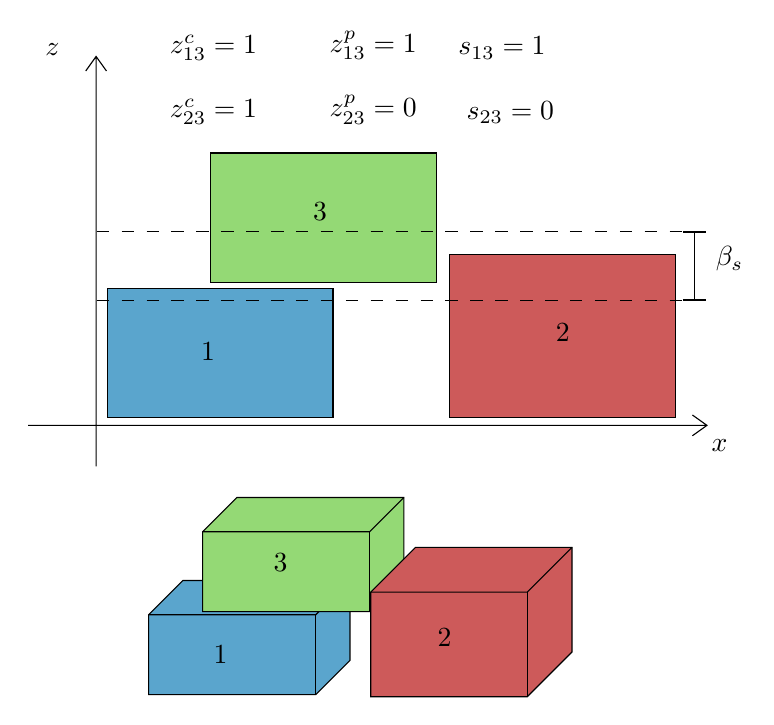
\begin{tikzpicture}[x=0.75pt,y=0.75pt,yscale=-1,xscale=1]
%uncomment if require: \path (0,438); %set diagram left start at 0, and has height of 438

%Shape: Axis 2D [id:dp1232896109350261] 
\draw  (168,199.75) -- (495,199.75)(200.7,22) -- (200.7,219.5) (488,194.75) -- (495,199.75) -- (488,204.75) (195.7,29) -- (200.7,22) -- (205.7,29)  ;
%Shape: Cube [id:dp2910169191165868] 
\draw  [fill={rgb, 255:red, 90; green, 165; blue, 205 }  ,fill opacity=1 ] (226,291) -- (242.5,274.5) -- (323,274.5) -- (323,313) -- (306.5,329.5) -- (226,329.5) -- cycle ; \draw   (323,274.5) -- (306.5,291) -- (226,291) ; \draw   (306.5,291) -- (306.5,329.5) ;
%Shape: Cube [id:dp8785627882196329] 
\draw  [fill={rgb, 255:red, 148; green, 217; blue, 117 }  ,fill opacity=1 ] (252,251) -- (268.5,234.5) -- (349,234.5) -- (349,273) -- (332.5,289.5) -- (252,289.5) -- cycle ; \draw   (349,234.5) -- (332.5,251) -- (252,251) ; \draw   (332.5,251) -- (332.5,289.5) ;
%Shape: Cube [id:dp9708534720424996] 
\draw  [fill={rgb, 255:red, 205; green, 90; blue, 90 }  ,fill opacity=1 ] (333,280.1) -- (354.6,258.5) -- (430,258.5) -- (430,308.9) -- (408.4,330.5) -- (333,330.5) -- cycle ; \draw   (430,258.5) -- (408.4,280.1) -- (333,280.1) ; \draw   (408.4,280.1) -- (408.4,330.5) ;
%Shape: Rectangle [id:dp1912318137049227] 
\draw  [fill={rgb, 255:red, 90; green, 165; blue, 205 }  ,fill opacity=1 ] (206,133.8) -- (314.84,133.8) -- (314.84,196) -- (206,196) -- cycle ;
%Shape: Rectangle [id:dp15878814114025752] 
\draw  [fill={rgb, 255:red, 148; green, 217; blue, 117 }  ,fill opacity=1 ] (255.76,68.5) -- (364.6,68.5) -- (364.6,130.7) -- (255.76,130.7) -- cycle ;
%Shape: Rectangle [id:dp45643376129890645] 
\draw  [fill={rgb, 255:red, 205; green, 90; blue, 90 }  ,fill opacity=1 ] (370.82,117.48) -- (479.66,117.48) -- (479.66,196) -- (370.82,196) -- cycle ;
%Straight Lines [id:da2605780157567503] 
\draw    (489,139.5) -- (489,106.5) ;
\draw [shift={(489,106.5)}, rotate = 90] [color={rgb, 255:red, 0; green, 0; blue, 0 }  ][line width=0.75]    (0,5.59) -- (0,-5.59)   ;
\draw [shift={(489,139.5)}, rotate = 90] [color={rgb, 255:red, 0; green, 0; blue, 0 }  ][line width=0.75]    (0,5.59) -- (0,-5.59)   ;
%Straight Lines [id:da24768955122380476] 
\draw  [dash pattern={on 4.5pt off 4.5pt}]  (201,139.5) -- (489,139.5) ;
%Straight Lines [id:da896443398249126] 
\draw  [dash pattern={on 4.5pt off 4.5pt}]  (201,106.5) -- (489,106.5) ;

% Text Node
\draw (496,205.4) node [anchor=north west][inner sep=0.75pt]    {$x$};
% Text Node
\draw (175,14.4) node [anchor=north west][inner sep=0.75pt]    {$z$};
% Text Node
\draw (498,112.4) node [anchor=north west][inner sep=0.75pt]    {$\beta _{s}$};
% Text Node
\draw (250,158.4) node [anchor=north west][inner sep=0.75pt]    {$1$};
% Text Node
\draw (421,149.4) node [anchor=north west][inner sep=0.75pt]    {$2$};
% Text Node
\draw (304,91.4) node [anchor=north west][inner sep=0.75pt]    {$3$};
% Text Node
\draw (235,10.4) node [anchor=north west][inner sep=0.75pt]    {$z_{13}^{c} =1$};
% Text Node
\draw (235,41.4) node [anchor=north west][inner sep=0.75pt]    {$z_{23}^{c} =1$};
% Text Node
\draw (312,8.4) node [anchor=north west][inner sep=0.75pt]    {$z_{13}^{p} =1$};
% Text Node
\draw (312,39.4) node [anchor=north west][inner sep=0.75pt]    {$z_{23}^{p} =0$};
% Text Node
\draw (374,11.4) node [anchor=north west][inner sep=0.75pt]    {$s_{13} =1$};
% Text Node
\draw (378,42.4) node [anchor=north west][inner sep=0.75pt]    {$s_{23} =0$};
% Text Node
\draw (256,304.4) node [anchor=north west][inner sep=0.75pt]    {$1$};
% Text Node
\draw (285,260.4) node [anchor=north west][inner sep=0.75pt]    {$3$};
% Text Node
\draw (364,296.4) node [anchor=north west][inner sep=0.75pt]    {$2$};


\end{tikzpicture}

                }
                \caption{Closeness variables example}
            \end{figure}

        \column{75mm}
            \resizebox{\columnwidth}{!}{
                \begin{minipage}{\linewidth}
                    \begin{align}
                        \text{s.t.} \qquad  & z_j - (z_i + h_i) \le \beta_s + H (1 - z^c_{ij}) & \forall (i, j) \in I : i \neq j \notag \\
                        & z_j - (z_i + h_i) \ge -\beta_s - H (1 - z^c_{ij}) & \forall (i, j) \in I : i \neq j \notag \\
                        & s_{ij} \le z^p_{ij} & \forall (i, j) \in I  \notag \\
                        & s_{ij} \le z^c_{ij} & \forall (i, j) \in I  \notag \\
                        & s_{ij} \ge z^p_{ij} + z^c_{ij} - 2 & \forall (i, j) \in I : i \neq j \notag \\
                        & \sum_{\mathclap{j \in I}}{s_{ij}} \le \sum_{\mathclap{b \in B}}{u_{ib}} & \forall i \in I  \notag
                    \end{align}
                \end{minipage}
            }
        \end{columns}
    \end{frame}

    \begin{frame}{MILP Proxy Model - Discretized Vertical Support}
        \begin{columns}[onlytextwidth,T]
            \column{\dimexpr\linewidth-75mm-5mm}
                \begin{figure}
                    \hspace*{-5mm}
                    \resizebox{1.35\columnwidth}{!}{
                        

\tikzset{every picture/.style={line width=0.75pt}} %set default line width to 0.75pt        

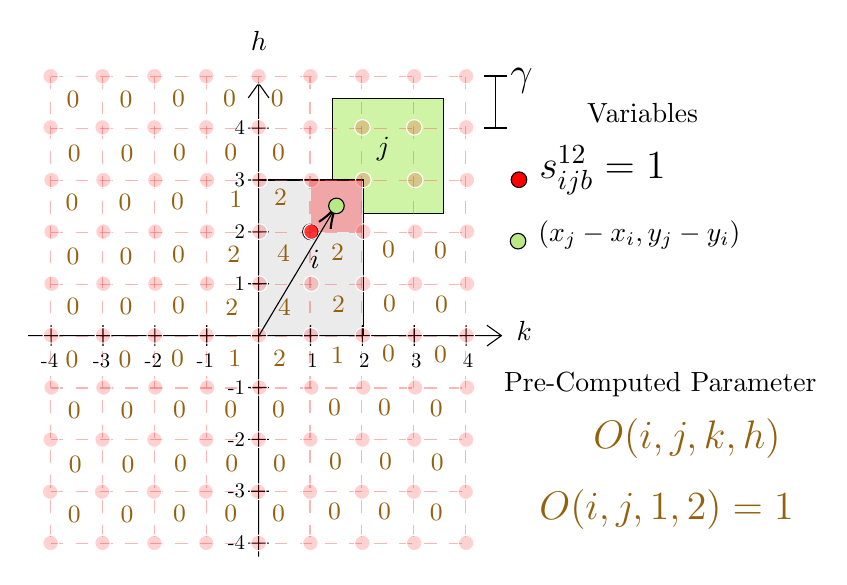
\begin{tikzpicture}[x=0.75pt,y=0.75pt,yscale=-1,xscale=1]
%uncomment if require: \path (0,300); %set diagram left start at 0, and has height of 300

%Shape: Rectangle [id:dp5959662237650998] 
\draw  [color={rgb, 255:red, 0; green, 0; blue, 0 }  ,draw opacity=1 ][fill={rgb, 255:red, 207; green, 244; blue, 165 }  ,fill opacity=1 ] (167.5,47.25) -- (221,47.25) -- (221,102.75) -- (167.5,102.75) -- cycle ;
%Shape: Rectangle [id:dp3153208771996219] 
\draw  [fill={rgb, 255:red, 235; green, 235; blue, 235 }  ,fill opacity=1 ] (132,86.5) -- (182.44,86.5) -- (182.44,161.5) -- (132,161.5) -- cycle ;
%Shape: Grid [id:dp3665057478133332] 
\draw  [draw opacity=0][fill={rgb, 255:red, 0; green, 0; blue, 0 }  ,fill opacity=0 ][dash pattern={on 4.5pt off 4.5pt}] (31.78,36.72) -- (232.78,36.72) -- (232.78,262.72) -- (31.78,262.72) -- cycle ; \draw  [color={rgb, 255:red, 247; green, 92; blue, 92 }  ,draw opacity=0.45 ][dash pattern={on 4.5pt off 4.5pt}] (31.78,36.72) -- (31.78,262.72)(56.78,36.72) -- (56.78,262.72)(81.78,36.72) -- (81.78,262.72)(106.78,36.72) -- (106.78,262.72)(131.78,36.72) -- (131.78,262.72)(156.78,36.72) -- (156.78,262.72)(181.78,36.72) -- (181.78,262.72)(206.78,36.72) -- (206.78,262.72)(231.78,36.72) -- (231.78,262.72) ; \draw  [color={rgb, 255:red, 247; green, 92; blue, 92 }  ,draw opacity=0.45 ][dash pattern={on 4.5pt off 4.5pt}] (31.78,36.72) -- (232.78,36.72)(31.78,61.72) -- (232.78,61.72)(31.78,86.72) -- (232.78,86.72)(31.78,111.72) -- (232.78,111.72)(31.78,136.72) -- (232.78,136.72)(31.78,161.72) -- (232.78,161.72)(31.78,186.72) -- (232.78,186.72)(31.78,211.72) -- (232.78,211.72)(31.78,236.72) -- (232.78,236.72)(31.78,261.72) -- (232.78,261.72) ; \draw  [color={rgb, 255:red, 247; green, 92; blue, 92 }  ,draw opacity=0.45 ][dash pattern={on 4.5pt off 4.5pt}]  ;
%Shape: Axis 2D [id:dp5870087683485721] 
\draw  (21,161.5) -- (249,161.5)(132,40) -- (132,268) (242,156.5) -- (249,161.5) -- (242,166.5) (127,47) -- (132,40) -- (137,47) (157,156.5) -- (157,166.5)(182,156.5) -- (182,166.5)(207,156.5) -- (207,166.5)(232,156.5) -- (232,166.5)(107,156.5) -- (107,166.5)(82,156.5) -- (82,166.5)(57,156.5) -- (57,166.5)(32,156.5) -- (32,166.5)(127,136.5) -- (137,136.5)(127,111.5) -- (137,111.5)(127,86.5) -- (137,86.5)(127,61.5) -- (137,61.5)(127,186.5) -- (137,186.5)(127,211.5) -- (137,211.5)(127,236.5) -- (137,236.5)(127,261.5) -- (137,261.5) ;
\draw   (164,173.5) node[anchor=east, scale=0.75]{1} (189,173.5) node[anchor=east, scale=0.75]{2} (214,173.5) node[anchor=east, scale=0.75]{3} (239,173.5) node[anchor=east, scale=0.75]{4} (114,173.5) node[anchor=east, scale=0.75]{-1} (89,173.5) node[anchor=east, scale=0.75]{-2} (64,173.5) node[anchor=east, scale=0.75]{-3} (39,173.5) node[anchor=east, scale=0.75]{-4} (129,136.5) node[anchor=east, scale=0.75]{1} (129,111.5) node[anchor=east, scale=0.75]{2} (129,86.5) node[anchor=east, scale=0.75]{3} (129,61.5) node[anchor=east, scale=0.75]{4} (129,186.5) node[anchor=east, scale=0.75]{-1} (129,211.5) node[anchor=east, scale=0.75]{-2} (129,236.5) node[anchor=east, scale=0.75]{-3} (129,261.5) node[anchor=east, scale=0.75]{-4} ;
%Straight Lines [id:da4474601658411276] 
\draw    (246,36.5) -- (246,61.5) ;
\draw [shift={(246,61.5)}, rotate = 270] [color={rgb, 255:red, 0; green, 0; blue, 0 }  ][line width=0.75]    (0,5.59) -- (0,-5.59)   ;
\draw [shift={(246,36.5)}, rotate = 270] [color={rgb, 255:red, 0; green, 0; blue, 0 }  ][line width=0.75]    (0,5.59) -- (0,-5.59)   ;
%Flowchart: Connector [id:dp17650433550879074] 
\draw  [color={rgb, 255:red, 255; green, 255; blue, 255 }  ,draw opacity=1 ][fill={rgb, 255:red, 255; green, 0; blue, 0 }  ,fill opacity=0.18 ] (28.03,36.5) .. controls (28.03,34.43) and (29.71,32.75) .. (31.78,32.75) .. controls (33.85,32.75) and (35.53,34.43) .. (35.53,36.5) .. controls (35.53,38.57) and (33.85,40.25) .. (31.78,40.25) .. controls (29.71,40.25) and (28.03,38.57) .. (28.03,36.5) -- cycle ;
%Flowchart: Connector [id:dp9770094792582217] 
\draw  [fill={rgb, 255:red, 255; green, 0; blue, 0 }  ,fill opacity=0.7 ] (153.25,111.5) .. controls (153.25,109.43) and (154.93,107.75) .. (157,107.75) .. controls (159.07,107.75) and (160.75,109.43) .. (160.75,111.5) .. controls (160.75,113.57) and (159.07,115.25) .. (157,115.25) .. controls (154.93,115.25) and (153.25,113.57) .. (153.25,111.5) -- cycle ;
%Flowchart: Connector [id:dp9315813149146155] 
\draw  [color={rgb, 255:red, 255; green, 255; blue, 255 }  ,draw opacity=1 ][fill={rgb, 255:red, 255; green, 0; blue, 0 }  ,fill opacity=0.18 ] (53.03,36.5) .. controls (53.03,34.43) and (54.71,32.75) .. (56.78,32.75) .. controls (58.85,32.75) and (60.53,34.43) .. (60.53,36.5) .. controls (60.53,38.57) and (58.85,40.25) .. (56.78,40.25) .. controls (54.71,40.25) and (53.03,38.57) .. (53.03,36.5) -- cycle ;
%Flowchart: Connector [id:dp8657956854954557] 
\draw  [color={rgb, 255:red, 255; green, 255; blue, 255 }  ,draw opacity=1 ][fill={rgb, 255:red, 255; green, 0; blue, 0 }  ,fill opacity=0.18 ] (78.03,36.5) .. controls (78.03,34.43) and (79.71,32.75) .. (81.78,32.75) .. controls (83.85,32.75) and (85.53,34.43) .. (85.53,36.5) .. controls (85.53,38.57) and (83.85,40.25) .. (81.78,40.25) .. controls (79.71,40.25) and (78.03,38.57) .. (78.03,36.5) -- cycle ;
%Flowchart: Connector [id:dp09342029252508777] 
\draw  [color={rgb, 255:red, 255; green, 255; blue, 255 }  ,draw opacity=1 ][fill={rgb, 255:red, 255; green, 0; blue, 0 }  ,fill opacity=0.18 ] (103.03,36.5) .. controls (103.03,34.43) and (104.71,32.75) .. (106.78,32.75) .. controls (108.85,32.75) and (110.53,34.43) .. (110.53,36.5) .. controls (110.53,38.57) and (108.85,40.25) .. (106.78,40.25) .. controls (104.71,40.25) and (103.03,38.57) .. (103.03,36.5) -- cycle ;
%Flowchart: Connector [id:dp533439523276273] 
\draw  [color={rgb, 255:red, 255; green, 255; blue, 255 }  ,draw opacity=1 ][fill={rgb, 255:red, 255; green, 0; blue, 0 }  ,fill opacity=0.18 ] (153.25,36.5) .. controls (153.25,34.43) and (154.93,32.75) .. (157,32.75) .. controls (159.07,32.75) and (160.75,34.43) .. (160.75,36.5) .. controls (160.75,38.57) and (159.07,40.25) .. (157,40.25) .. controls (154.93,40.25) and (153.25,38.57) .. (153.25,36.5) -- cycle ;
%Flowchart: Connector [id:dp17730485501604987] 
\draw  [color={rgb, 255:red, 255; green, 255; blue, 255 }  ,draw opacity=1 ][fill={rgb, 255:red, 255; green, 0; blue, 0 }  ,fill opacity=0.18 ] (178.25,36.5) .. controls (178.25,34.43) and (179.93,32.75) .. (182,32.75) .. controls (184.07,32.75) and (185.75,34.43) .. (185.75,36.5) .. controls (185.75,38.57) and (184.07,40.25) .. (182,40.25) .. controls (179.93,40.25) and (178.25,38.57) .. (178.25,36.5) -- cycle ;
%Flowchart: Connector [id:dp8819775226725283] 
\draw  [color={rgb, 255:red, 255; green, 255; blue, 255 }  ,draw opacity=1 ][fill={rgb, 255:red, 255; green, 0; blue, 0 }  ,fill opacity=0.18 ] (203.25,36.5) .. controls (203.25,34.43) and (204.93,32.75) .. (207,32.75) .. controls (209.07,32.75) and (210.75,34.43) .. (210.75,36.5) .. controls (210.75,38.57) and (209.07,40.25) .. (207,40.25) .. controls (204.93,40.25) and (203.25,38.57) .. (203.25,36.5) -- cycle ;
%Flowchart: Connector [id:dp1420881048740692] 
\draw  [color={rgb, 255:red, 255; green, 255; blue, 255 }  ,draw opacity=1 ][fill={rgb, 255:red, 255; green, 0; blue, 0 }  ,fill opacity=0.18 ] (228.25,36.5) .. controls (228.25,34.43) and (229.93,32.75) .. (232,32.75) .. controls (234.07,32.75) and (235.75,34.43) .. (235.75,36.5) .. controls (235.75,38.57) and (234.07,40.25) .. (232,40.25) .. controls (229.93,40.25) and (228.25,38.57) .. (228.25,36.5) -- cycle ;
%Flowchart: Connector [id:dp014549534119622898] 
\draw  [color={rgb, 255:red, 255; green, 255; blue, 255 }  ,draw opacity=1 ][fill={rgb, 255:red, 255; green, 0; blue, 0 }  ,fill opacity=0.18 ] (128.25,36.5) .. controls (128.25,34.43) and (129.93,32.75) .. (132,32.75) .. controls (134.07,32.75) and (135.75,34.43) .. (135.75,36.5) .. controls (135.75,38.57) and (134.07,40.25) .. (132,40.25) .. controls (129.93,40.25) and (128.25,38.57) .. (128.25,36.5) -- cycle ;
%Flowchart: Connector [id:dp5842977340969858] 
\draw  [color={rgb, 255:red, 255; green, 255; blue, 255 }  ,draw opacity=1 ][fill={rgb, 255:red, 255; green, 0; blue, 0 }  ,fill opacity=0.18 ] (28.03,61.17) .. controls (28.03,59.1) and (29.71,57.42) .. (31.78,57.42) .. controls (33.85,57.42) and (35.53,59.1) .. (35.53,61.17) .. controls (35.53,63.24) and (33.85,64.92) .. (31.78,64.92) .. controls (29.71,64.92) and (28.03,63.24) .. (28.03,61.17) -- cycle ;
%Flowchart: Connector [id:dp6519155112808065] 
\draw  [color={rgb, 255:red, 255; green, 255; blue, 255 }  ,draw opacity=1 ][fill={rgb, 255:red, 255; green, 0; blue, 0 }  ,fill opacity=0.18 ] (53.03,61.17) .. controls (53.03,59.1) and (54.71,57.42) .. (56.78,57.42) .. controls (58.85,57.42) and (60.53,59.1) .. (60.53,61.17) .. controls (60.53,63.24) and (58.85,64.92) .. (56.78,64.92) .. controls (54.71,64.92) and (53.03,63.24) .. (53.03,61.17) -- cycle ;
%Flowchart: Connector [id:dp36077536920560327] 
\draw  [color={rgb, 255:red, 255; green, 255; blue, 255 }  ,draw opacity=1 ][fill={rgb, 255:red, 255; green, 0; blue, 0 }  ,fill opacity=0.18 ] (78.03,61.17) .. controls (78.03,59.1) and (79.71,57.42) .. (81.78,57.42) .. controls (83.85,57.42) and (85.53,59.1) .. (85.53,61.17) .. controls (85.53,63.24) and (83.85,64.92) .. (81.78,64.92) .. controls (79.71,64.92) and (78.03,63.24) .. (78.03,61.17) -- cycle ;
%Flowchart: Connector [id:dp5189088045367096] 
\draw  [color={rgb, 255:red, 255; green, 255; blue, 255 }  ,draw opacity=1 ][fill={rgb, 255:red, 255; green, 0; blue, 0 }  ,fill opacity=0.18 ] (103.03,61.17) .. controls (103.03,59.1) and (104.71,57.42) .. (106.78,57.42) .. controls (108.85,57.42) and (110.53,59.1) .. (110.53,61.17) .. controls (110.53,63.24) and (108.85,64.92) .. (106.78,64.92) .. controls (104.71,64.92) and (103.03,63.24) .. (103.03,61.17) -- cycle ;
%Flowchart: Connector [id:dp05741768855482643] 
\draw  [color={rgb, 255:red, 255; green, 255; blue, 255 }  ,draw opacity=1 ][fill={rgb, 255:red, 255; green, 0; blue, 0 }  ,fill opacity=0.18 ] (153.25,61.17) .. controls (153.25,59.1) and (154.93,57.42) .. (157,57.42) .. controls (159.07,57.42) and (160.75,59.1) .. (160.75,61.17) .. controls (160.75,63.24) and (159.07,64.92) .. (157,64.92) .. controls (154.93,64.92) and (153.25,63.24) .. (153.25,61.17) -- cycle ;
%Flowchart: Connector [id:dp006363561960593622] 
\draw  [color={rgb, 255:red, 255; green, 255; blue, 255 }  ,draw opacity=1 ][fill={rgb, 255:red, 255; green, 0; blue, 0 }  ,fill opacity=0.18 ] (178.25,61.17) .. controls (178.25,59.1) and (179.93,57.42) .. (182,57.42) .. controls (184.07,57.42) and (185.75,59.1) .. (185.75,61.17) .. controls (185.75,63.24) and (184.07,64.92) .. (182,64.92) .. controls (179.93,64.92) and (178.25,63.24) .. (178.25,61.17) -- cycle ;
%Flowchart: Connector [id:dp46345859900758] 
\draw  [color={rgb, 255:red, 255; green, 255; blue, 255 }  ,draw opacity=1 ][fill={rgb, 255:red, 255; green, 0; blue, 0 }  ,fill opacity=0.18 ] (203.25,61.17) .. controls (203.25,59.1) and (204.93,57.42) .. (207,57.42) .. controls (209.07,57.42) and (210.75,59.1) .. (210.75,61.17) .. controls (210.75,63.24) and (209.07,64.92) .. (207,64.92) .. controls (204.93,64.92) and (203.25,63.24) .. (203.25,61.17) -- cycle ;
%Flowchart: Connector [id:dp019098380251666325] 
\draw  [color={rgb, 255:red, 255; green, 255; blue, 255 }  ,draw opacity=1 ][fill={rgb, 255:red, 255; green, 0; blue, 0 }  ,fill opacity=0.18 ] (228.25,61.17) .. controls (228.25,59.1) and (229.93,57.42) .. (232,57.42) .. controls (234.07,57.42) and (235.75,59.1) .. (235.75,61.17) .. controls (235.75,63.24) and (234.07,64.92) .. (232,64.92) .. controls (229.93,64.92) and (228.25,63.24) .. (228.25,61.17) -- cycle ;
%Flowchart: Connector [id:dp8272679894580149] 
\draw  [color={rgb, 255:red, 255; green, 255; blue, 255 }  ,draw opacity=1 ][fill={rgb, 255:red, 255; green, 0; blue, 0 }  ,fill opacity=0.18 ] (128.25,61.17) .. controls (128.25,59.1) and (129.93,57.42) .. (132,57.42) .. controls (134.07,57.42) and (135.75,59.1) .. (135.75,61.17) .. controls (135.75,63.24) and (134.07,64.92) .. (132,64.92) .. controls (129.93,64.92) and (128.25,63.24) .. (128.25,61.17) -- cycle ;
%Flowchart: Connector [id:dp01549254055562177] 
\draw  [color={rgb, 255:red, 255; green, 255; blue, 255 }  ,draw opacity=1 ][fill={rgb, 255:red, 255; green, 0; blue, 0 }  ,fill opacity=0.18 ] (28.47,86.5) .. controls (28.47,84.43) and (30.15,82.75) .. (32.22,82.75) .. controls (34.29,82.75) and (35.97,84.43) .. (35.97,86.5) .. controls (35.97,88.57) and (34.29,90.25) .. (32.22,90.25) .. controls (30.15,90.25) and (28.47,88.57) .. (28.47,86.5) -- cycle ;
%Flowchart: Connector [id:dp027166291716461677] 
\draw  [color={rgb, 255:red, 255; green, 255; blue, 255 }  ,draw opacity=1 ][fill={rgb, 255:red, 255; green, 0; blue, 0 }  ,fill opacity=0.18 ] (53.47,86.5) .. controls (53.47,84.43) and (55.15,82.75) .. (57.22,82.75) .. controls (59.29,82.75) and (60.97,84.43) .. (60.97,86.5) .. controls (60.97,88.57) and (59.29,90.25) .. (57.22,90.25) .. controls (55.15,90.25) and (53.47,88.57) .. (53.47,86.5) -- cycle ;
%Flowchart: Connector [id:dp8515274344244661] 
\draw  [color={rgb, 255:red, 255; green, 255; blue, 255 }  ,draw opacity=1 ][fill={rgb, 255:red, 255; green, 0; blue, 0 }  ,fill opacity=0.18 ] (78.47,86.5) .. controls (78.47,84.43) and (80.15,82.75) .. (82.22,82.75) .. controls (84.29,82.75) and (85.97,84.43) .. (85.97,86.5) .. controls (85.97,88.57) and (84.29,90.25) .. (82.22,90.25) .. controls (80.15,90.25) and (78.47,88.57) .. (78.47,86.5) -- cycle ;
%Flowchart: Connector [id:dp20327157268330664] 
\draw  [color={rgb, 255:red, 255; green, 255; blue, 255 }  ,draw opacity=1 ][fill={rgb, 255:red, 255; green, 0; blue, 0 }  ,fill opacity=0.18 ] (103.47,86.5) .. controls (103.47,84.43) and (105.15,82.75) .. (107.22,82.75) .. controls (109.29,82.75) and (110.97,84.43) .. (110.97,86.5) .. controls (110.97,88.57) and (109.29,90.25) .. (107.22,90.25) .. controls (105.15,90.25) and (103.47,88.57) .. (103.47,86.5) -- cycle ;
%Flowchart: Connector [id:dp13376132351948555] 
\draw  [color={rgb, 255:red, 255; green, 255; blue, 255 }  ,draw opacity=1 ][fill={rgb, 255:red, 255; green, 0; blue, 0 }  ,fill opacity=0.18 ] (153.69,86.5) .. controls (153.69,84.43) and (155.37,82.75) .. (157.44,82.75) .. controls (159.52,82.75) and (161.19,84.43) .. (161.19,86.5) .. controls (161.19,88.57) and (159.52,90.25) .. (157.44,90.25) .. controls (155.37,90.25) and (153.69,88.57) .. (153.69,86.5) -- cycle ;
%Flowchart: Connector [id:dp4044064224279934] 
\draw  [color={rgb, 255:red, 255; green, 255; blue, 255 }  ,draw opacity=1 ][fill={rgb, 255:red, 255; green, 0; blue, 0 }  ,fill opacity=0.18 ] (178.69,86.5) .. controls (178.69,84.43) and (180.37,82.75) .. (182.44,82.75) .. controls (184.52,82.75) and (186.19,84.43) .. (186.19,86.5) .. controls (186.19,88.57) and (184.52,90.25) .. (182.44,90.25) .. controls (180.37,90.25) and (178.69,88.57) .. (178.69,86.5) -- cycle ;
%Flowchart: Connector [id:dp07583386051229557] 
\draw  [color={rgb, 255:red, 255; green, 255; blue, 255 }  ,draw opacity=1 ][fill={rgb, 255:red, 255; green, 0; blue, 0 }  ,fill opacity=0.18 ] (203.69,86.5) .. controls (203.69,84.43) and (205.37,82.75) .. (207.44,82.75) .. controls (209.52,82.75) and (211.19,84.43) .. (211.19,86.5) .. controls (211.19,88.57) and (209.52,90.25) .. (207.44,90.25) .. controls (205.37,90.25) and (203.69,88.57) .. (203.69,86.5) -- cycle ;
%Flowchart: Connector [id:dp49124263363886067] 
\draw  [color={rgb, 255:red, 255; green, 255; blue, 255 }  ,draw opacity=1 ][fill={rgb, 255:red, 255; green, 0; blue, 0 }  ,fill opacity=0.18 ] (228.69,86.5) .. controls (228.69,84.43) and (230.37,82.75) .. (232.44,82.75) .. controls (234.52,82.75) and (236.19,84.43) .. (236.19,86.5) .. controls (236.19,88.57) and (234.52,90.25) .. (232.44,90.25) .. controls (230.37,90.25) and (228.69,88.57) .. (228.69,86.5) -- cycle ;
%Flowchart: Connector [id:dp8856760470116622] 
\draw  [color={rgb, 255:red, 255; green, 255; blue, 255 }  ,draw opacity=1 ][fill={rgb, 255:red, 255; green, 0; blue, 0 }  ,fill opacity=0.18 ] (128.69,86.5) .. controls (128.69,84.43) and (130.37,82.75) .. (132.44,82.75) .. controls (134.52,82.75) and (136.19,84.43) .. (136.19,86.5) .. controls (136.19,88.57) and (134.52,90.25) .. (132.44,90.25) .. controls (130.37,90.25) and (128.69,88.57) .. (128.69,86.5) -- cycle ;
%Flowchart: Connector [id:dp301207315319171] 
\draw  [color={rgb, 255:red, 255; green, 255; blue, 255 }  ,draw opacity=1 ][fill={rgb, 255:red, 255; green, 0; blue, 0 }  ,fill opacity=0.18 ] (28.47,111.39) .. controls (28.47,109.32) and (30.15,107.64) .. (32.22,107.64) .. controls (34.29,107.64) and (35.97,109.32) .. (35.97,111.39) .. controls (35.97,113.46) and (34.29,115.14) .. (32.22,115.14) .. controls (30.15,115.14) and (28.47,113.46) .. (28.47,111.39) -- cycle ;
%Flowchart: Connector [id:dp9873901030687902] 
\draw  [color={rgb, 255:red, 255; green, 255; blue, 255 }  ,draw opacity=1 ][fill={rgb, 255:red, 255; green, 0; blue, 0 }  ,fill opacity=0.18 ] (53.47,111.39) .. controls (53.47,109.32) and (55.15,107.64) .. (57.22,107.64) .. controls (59.29,107.64) and (60.97,109.32) .. (60.97,111.39) .. controls (60.97,113.46) and (59.29,115.14) .. (57.22,115.14) .. controls (55.15,115.14) and (53.47,113.46) .. (53.47,111.39) -- cycle ;
%Flowchart: Connector [id:dp5933980597190441] 
\draw  [color={rgb, 255:red, 255; green, 255; blue, 255 }  ,draw opacity=1 ][fill={rgb, 255:red, 255; green, 0; blue, 0 }  ,fill opacity=0.18 ] (78.47,111.39) .. controls (78.47,109.32) and (80.15,107.64) .. (82.22,107.64) .. controls (84.29,107.64) and (85.97,109.32) .. (85.97,111.39) .. controls (85.97,113.46) and (84.29,115.14) .. (82.22,115.14) .. controls (80.15,115.14) and (78.47,113.46) .. (78.47,111.39) -- cycle ;
%Flowchart: Connector [id:dp0845756744343803] 
\draw  [color={rgb, 255:red, 255; green, 255; blue, 255 }  ,draw opacity=1 ][fill={rgb, 255:red, 255; green, 0; blue, 0 }  ,fill opacity=0.18 ] (103.47,111.39) .. controls (103.47,109.32) and (105.15,107.64) .. (107.22,107.64) .. controls (109.29,107.64) and (110.97,109.32) .. (110.97,111.39) .. controls (110.97,113.46) and (109.29,115.14) .. (107.22,115.14) .. controls (105.15,115.14) and (103.47,113.46) .. (103.47,111.39) -- cycle ;
%Flowchart: Connector [id:dp29502546476584324] 
\draw  [color={rgb, 255:red, 255; green, 255; blue, 255 }  ,draw opacity=1 ][fill={rgb, 255:red, 255; green, 0; blue, 0 }  ,fill opacity=0.18 ] (153.69,111.39) .. controls (153.69,109.32) and (155.37,107.64) .. (157.44,107.64) .. controls (159.52,107.64) and (161.19,109.32) .. (161.19,111.39) .. controls (161.19,113.46) and (159.52,115.14) .. (157.44,115.14) .. controls (155.37,115.14) and (153.69,113.46) .. (153.69,111.39) -- cycle ;
%Flowchart: Connector [id:dp06874296669968716] 
\draw  [color={rgb, 255:red, 255; green, 255; blue, 255 }  ,draw opacity=1 ][fill={rgb, 255:red, 255; green, 0; blue, 0 }  ,fill opacity=0.18 ] (178.69,111.39) .. controls (178.69,109.32) and (180.37,107.64) .. (182.44,107.64) .. controls (184.52,107.64) and (186.19,109.32) .. (186.19,111.39) .. controls (186.19,113.46) and (184.52,115.14) .. (182.44,115.14) .. controls (180.37,115.14) and (178.69,113.46) .. (178.69,111.39) -- cycle ;
%Flowchart: Connector [id:dp9162544207566379] 
\draw  [color={rgb, 255:red, 255; green, 255; blue, 255 }  ,draw opacity=1 ][fill={rgb, 255:red, 255; green, 0; blue, 0 }  ,fill opacity=0.18 ] (203.69,111.39) .. controls (203.69,109.32) and (205.37,107.64) .. (207.44,107.64) .. controls (209.52,107.64) and (211.19,109.32) .. (211.19,111.39) .. controls (211.19,113.46) and (209.52,115.14) .. (207.44,115.14) .. controls (205.37,115.14) and (203.69,113.46) .. (203.69,111.39) -- cycle ;
%Flowchart: Connector [id:dp14989652582386304] 
\draw  [color={rgb, 255:red, 255; green, 255; blue, 255 }  ,draw opacity=1 ][fill={rgb, 255:red, 255; green, 0; blue, 0 }  ,fill opacity=0.18 ] (228.69,111.39) .. controls (228.69,109.32) and (230.37,107.64) .. (232.44,107.64) .. controls (234.52,107.64) and (236.19,109.32) .. (236.19,111.39) .. controls (236.19,113.46) and (234.52,115.14) .. (232.44,115.14) .. controls (230.37,115.14) and (228.69,113.46) .. (228.69,111.39) -- cycle ;
%Flowchart: Connector [id:dp3853078344508225] 
\draw  [color={rgb, 255:red, 255; green, 255; blue, 255 }  ,draw opacity=1 ][fill={rgb, 255:red, 255; green, 0; blue, 0 }  ,fill opacity=0.18 ] (128.69,111.39) .. controls (128.69,109.32) and (130.37,107.64) .. (132.44,107.64) .. controls (134.52,107.64) and (136.19,109.32) .. (136.19,111.39) .. controls (136.19,113.46) and (134.52,115.14) .. (132.44,115.14) .. controls (130.37,115.14) and (128.69,113.46) .. (128.69,111.39) -- cycle ;
%Flowchart: Connector [id:dp7343580941980375] 
\draw  [color={rgb, 255:red, 255; green, 255; blue, 255 }  ,draw opacity=1 ][fill={rgb, 255:red, 255; green, 0; blue, 0 }  ,fill opacity=0.18 ] (28.47,136.5) .. controls (28.47,134.43) and (30.15,132.75) .. (32.22,132.75) .. controls (34.29,132.75) and (35.97,134.43) .. (35.97,136.5) .. controls (35.97,138.57) and (34.29,140.25) .. (32.22,140.25) .. controls (30.15,140.25) and (28.47,138.57) .. (28.47,136.5) -- cycle ;
%Flowchart: Connector [id:dp5897030420385775] 
\draw  [color={rgb, 255:red, 255; green, 255; blue, 255 }  ,draw opacity=1 ][fill={rgb, 255:red, 255; green, 0; blue, 0 }  ,fill opacity=0.18 ] (53.47,136.5) .. controls (53.47,134.43) and (55.15,132.75) .. (57.22,132.75) .. controls (59.29,132.75) and (60.97,134.43) .. (60.97,136.5) .. controls (60.97,138.57) and (59.29,140.25) .. (57.22,140.25) .. controls (55.15,140.25) and (53.47,138.57) .. (53.47,136.5) -- cycle ;
%Flowchart: Connector [id:dp4113531826732052] 
\draw  [color={rgb, 255:red, 255; green, 255; blue, 255 }  ,draw opacity=1 ][fill={rgb, 255:red, 255; green, 0; blue, 0 }  ,fill opacity=0.18 ] (78.47,136.5) .. controls (78.47,134.43) and (80.15,132.75) .. (82.22,132.75) .. controls (84.29,132.75) and (85.97,134.43) .. (85.97,136.5) .. controls (85.97,138.57) and (84.29,140.25) .. (82.22,140.25) .. controls (80.15,140.25) and (78.47,138.57) .. (78.47,136.5) -- cycle ;
%Flowchart: Connector [id:dp23228874377402398] 
\draw  [color={rgb, 255:red, 255; green, 255; blue, 255 }  ,draw opacity=1 ][fill={rgb, 255:red, 255; green, 0; blue, 0 }  ,fill opacity=0.18 ] (103.47,136.5) .. controls (103.47,134.43) and (105.15,132.75) .. (107.22,132.75) .. controls (109.29,132.75) and (110.97,134.43) .. (110.97,136.5) .. controls (110.97,138.57) and (109.29,140.25) .. (107.22,140.25) .. controls (105.15,140.25) and (103.47,138.57) .. (103.47,136.5) -- cycle ;
%Flowchart: Connector [id:dp6880757085593899] 
\draw  [color={rgb, 255:red, 255; green, 255; blue, 255 }  ,draw opacity=1 ][fill={rgb, 255:red, 255; green, 0; blue, 0 }  ,fill opacity=0.18 ] (153.69,136.5) .. controls (153.69,134.43) and (155.37,132.75) .. (157.44,132.75) .. controls (159.52,132.75) and (161.19,134.43) .. (161.19,136.5) .. controls (161.19,138.57) and (159.52,140.25) .. (157.44,140.25) .. controls (155.37,140.25) and (153.69,138.57) .. (153.69,136.5) -- cycle ;
%Flowchart: Connector [id:dp11022600404271554] 
\draw  [color={rgb, 255:red, 255; green, 255; blue, 255 }  ,draw opacity=1 ][fill={rgb, 255:red, 255; green, 0; blue, 0 }  ,fill opacity=0.18 ] (178.69,136.5) .. controls (178.69,134.43) and (180.37,132.75) .. (182.44,132.75) .. controls (184.52,132.75) and (186.19,134.43) .. (186.19,136.5) .. controls (186.19,138.57) and (184.52,140.25) .. (182.44,140.25) .. controls (180.37,140.25) and (178.69,138.57) .. (178.69,136.5) -- cycle ;
%Flowchart: Connector [id:dp3137776827032247] 
\draw  [color={rgb, 255:red, 255; green, 255; blue, 255 }  ,draw opacity=1 ][fill={rgb, 255:red, 255; green, 0; blue, 0 }  ,fill opacity=0.18 ] (203.69,136.5) .. controls (203.69,134.43) and (205.37,132.75) .. (207.44,132.75) .. controls (209.52,132.75) and (211.19,134.43) .. (211.19,136.5) .. controls (211.19,138.57) and (209.52,140.25) .. (207.44,140.25) .. controls (205.37,140.25) and (203.69,138.57) .. (203.69,136.5) -- cycle ;
%Flowchart: Connector [id:dp9734591452399853] 
\draw  [color={rgb, 255:red, 255; green, 255; blue, 255 }  ,draw opacity=1 ][fill={rgb, 255:red, 255; green, 0; blue, 0 }  ,fill opacity=0.18 ] (228.69,136.5) .. controls (228.69,134.43) and (230.37,132.75) .. (232.44,132.75) .. controls (234.52,132.75) and (236.19,134.43) .. (236.19,136.5) .. controls (236.19,138.57) and (234.52,140.25) .. (232.44,140.25) .. controls (230.37,140.25) and (228.69,138.57) .. (228.69,136.5) -- cycle ;
%Flowchart: Connector [id:dp6232488894599273] 
\draw  [color={rgb, 255:red, 255; green, 255; blue, 255 }  ,draw opacity=1 ][fill={rgb, 255:red, 255; green, 0; blue, 0 }  ,fill opacity=0.18 ] (128.69,136.5) .. controls (128.69,134.43) and (130.37,132.75) .. (132.44,132.75) .. controls (134.52,132.75) and (136.19,134.43) .. (136.19,136.5) .. controls (136.19,138.57) and (134.52,140.25) .. (132.44,140.25) .. controls (130.37,140.25) and (128.69,138.57) .. (128.69,136.5) -- cycle ;
%Flowchart: Connector [id:dp3478090854930638] 
\draw  [color={rgb, 255:red, 255; green, 255; blue, 255 }  ,draw opacity=1 ][fill={rgb, 255:red, 255; green, 0; blue, 0 }  ,fill opacity=0.18 ] (28.25,161.39) .. controls (28.25,159.32) and (29.93,157.64) .. (32,157.64) .. controls (34.07,157.64) and (35.75,159.32) .. (35.75,161.39) .. controls (35.75,163.46) and (34.07,165.14) .. (32,165.14) .. controls (29.93,165.14) and (28.25,163.46) .. (28.25,161.39) -- cycle ;
%Flowchart: Connector [id:dp35688119374307803] 
\draw  [color={rgb, 255:red, 255; green, 255; blue, 255 }  ,draw opacity=1 ][fill={rgb, 255:red, 255; green, 0; blue, 0 }  ,fill opacity=0.18 ] (53.25,161.39) .. controls (53.25,159.32) and (54.93,157.64) .. (57,157.64) .. controls (59.07,157.64) and (60.75,159.32) .. (60.75,161.39) .. controls (60.75,163.46) and (59.07,165.14) .. (57,165.14) .. controls (54.93,165.14) and (53.25,163.46) .. (53.25,161.39) -- cycle ;
%Flowchart: Connector [id:dp08842159328353927] 
\draw  [color={rgb, 255:red, 255; green, 255; blue, 255 }  ,draw opacity=1 ][fill={rgb, 255:red, 255; green, 0; blue, 0 }  ,fill opacity=0.18 ] (78.25,161.39) .. controls (78.25,159.32) and (79.93,157.64) .. (82,157.64) .. controls (84.07,157.64) and (85.75,159.32) .. (85.75,161.39) .. controls (85.75,163.46) and (84.07,165.14) .. (82,165.14) .. controls (79.93,165.14) and (78.25,163.46) .. (78.25,161.39) -- cycle ;
%Flowchart: Connector [id:dp2970957139814403] 
\draw  [color={rgb, 255:red, 255; green, 255; blue, 255 }  ,draw opacity=1 ][fill={rgb, 255:red, 255; green, 0; blue, 0 }  ,fill opacity=0.18 ] (103.25,161.39) .. controls (103.25,159.32) and (104.93,157.64) .. (107,157.64) .. controls (109.07,157.64) and (110.75,159.32) .. (110.75,161.39) .. controls (110.75,163.46) and (109.07,165.14) .. (107,165.14) .. controls (104.93,165.14) and (103.25,163.46) .. (103.25,161.39) -- cycle ;
%Flowchart: Connector [id:dp48068406879743175] 
\draw  [color={rgb, 255:red, 255; green, 255; blue, 255 }  ,draw opacity=1 ][fill={rgb, 255:red, 255; green, 0; blue, 0 }  ,fill opacity=0.18 ] (153.47,161.39) .. controls (153.47,159.32) and (155.15,157.64) .. (157.22,157.64) .. controls (159.29,157.64) and (160.97,159.32) .. (160.97,161.39) .. controls (160.97,163.46) and (159.29,165.14) .. (157.22,165.14) .. controls (155.15,165.14) and (153.47,163.46) .. (153.47,161.39) -- cycle ;
%Flowchart: Connector [id:dp6749856184628993] 
\draw  [color={rgb, 255:red, 255; green, 255; blue, 255 }  ,draw opacity=1 ][fill={rgb, 255:red, 255; green, 0; blue, 0 }  ,fill opacity=0.18 ] (178.47,161.39) .. controls (178.47,159.32) and (180.15,157.64) .. (182.22,157.64) .. controls (184.29,157.64) and (185.97,159.32) .. (185.97,161.39) .. controls (185.97,163.46) and (184.29,165.14) .. (182.22,165.14) .. controls (180.15,165.14) and (178.47,163.46) .. (178.47,161.39) -- cycle ;
%Flowchart: Connector [id:dp47756572698239763] 
\draw  [color={rgb, 255:red, 255; green, 255; blue, 255 }  ,draw opacity=1 ][fill={rgb, 255:red, 255; green, 0; blue, 0 }  ,fill opacity=0.18 ] (203.47,161.39) .. controls (203.47,159.32) and (205.15,157.64) .. (207.22,157.64) .. controls (209.29,157.64) and (210.97,159.32) .. (210.97,161.39) .. controls (210.97,163.46) and (209.29,165.14) .. (207.22,165.14) .. controls (205.15,165.14) and (203.47,163.46) .. (203.47,161.39) -- cycle ;
%Flowchart: Connector [id:dp04509105985203821] 
\draw  [color={rgb, 255:red, 255; green, 255; blue, 255 }  ,draw opacity=1 ][fill={rgb, 255:red, 255; green, 0; blue, 0 }  ,fill opacity=0.18 ] (228.47,161.39) .. controls (228.47,159.32) and (230.15,157.64) .. (232.22,157.64) .. controls (234.29,157.64) and (235.97,159.32) .. (235.97,161.39) .. controls (235.97,163.46) and (234.29,165.14) .. (232.22,165.14) .. controls (230.15,165.14) and (228.47,163.46) .. (228.47,161.39) -- cycle ;
%Flowchart: Connector [id:dp8683592527953342] 
\draw  [color={rgb, 255:red, 255; green, 255; blue, 255 }  ,draw opacity=1 ][fill={rgb, 255:red, 255; green, 0; blue, 0 }  ,fill opacity=0.18 ] (128.47,161.39) .. controls (128.47,159.32) and (130.15,157.64) .. (132.22,157.64) .. controls (134.29,157.64) and (135.97,159.32) .. (135.97,161.39) .. controls (135.97,163.46) and (134.29,165.14) .. (132.22,165.14) .. controls (130.15,165.14) and (128.47,163.46) .. (128.47,161.39) -- cycle ;
%Flowchart: Connector [id:dp3038506526517001] 
\draw  [color={rgb, 255:red, 255; green, 255; blue, 255 }  ,draw opacity=1 ][fill={rgb, 255:red, 255; green, 0; blue, 0 }  ,fill opacity=0.18 ] (28.47,186.5) .. controls (28.47,184.43) and (30.15,182.75) .. (32.22,182.75) .. controls (34.29,182.75) and (35.97,184.43) .. (35.97,186.5) .. controls (35.97,188.57) and (34.29,190.25) .. (32.22,190.25) .. controls (30.15,190.25) and (28.47,188.57) .. (28.47,186.5) -- cycle ;
%Flowchart: Connector [id:dp6172754428181076] 
\draw  [color={rgb, 255:red, 255; green, 255; blue, 255 }  ,draw opacity=1 ][fill={rgb, 255:red, 255; green, 0; blue, 0 }  ,fill opacity=0.18 ] (53.47,186.5) .. controls (53.47,184.43) and (55.15,182.75) .. (57.22,182.75) .. controls (59.29,182.75) and (60.97,184.43) .. (60.97,186.5) .. controls (60.97,188.57) and (59.29,190.25) .. (57.22,190.25) .. controls (55.15,190.25) and (53.47,188.57) .. (53.47,186.5) -- cycle ;
%Flowchart: Connector [id:dp013991251264403148] 
\draw  [color={rgb, 255:red, 255; green, 255; blue, 255 }  ,draw opacity=1 ][fill={rgb, 255:red, 255; green, 0; blue, 0 }  ,fill opacity=0.18 ] (78.47,186.5) .. controls (78.47,184.43) and (80.15,182.75) .. (82.22,182.75) .. controls (84.29,182.75) and (85.97,184.43) .. (85.97,186.5) .. controls (85.97,188.57) and (84.29,190.25) .. (82.22,190.25) .. controls (80.15,190.25) and (78.47,188.57) .. (78.47,186.5) -- cycle ;
%Flowchart: Connector [id:dp6293436045141049] 
\draw  [color={rgb, 255:red, 255; green, 255; blue, 255 }  ,draw opacity=1 ][fill={rgb, 255:red, 255; green, 0; blue, 0 }  ,fill opacity=0.18 ] (103.47,186.5) .. controls (103.47,184.43) and (105.15,182.75) .. (107.22,182.75) .. controls (109.29,182.75) and (110.97,184.43) .. (110.97,186.5) .. controls (110.97,188.57) and (109.29,190.25) .. (107.22,190.25) .. controls (105.15,190.25) and (103.47,188.57) .. (103.47,186.5) -- cycle ;
%Flowchart: Connector [id:dp7429597573459572] 
\draw  [color={rgb, 255:red, 255; green, 255; blue, 255 }  ,draw opacity=1 ][fill={rgb, 255:red, 255; green, 0; blue, 0 }  ,fill opacity=0.18 ] (153.69,186.5) .. controls (153.69,184.43) and (155.37,182.75) .. (157.44,182.75) .. controls (159.52,182.75) and (161.19,184.43) .. (161.19,186.5) .. controls (161.19,188.57) and (159.52,190.25) .. (157.44,190.25) .. controls (155.37,190.25) and (153.69,188.57) .. (153.69,186.5) -- cycle ;
%Flowchart: Connector [id:dp7880373269123602] 
\draw  [color={rgb, 255:red, 255; green, 255; blue, 255 }  ,draw opacity=1 ][fill={rgb, 255:red, 255; green, 0; blue, 0 }  ,fill opacity=0.18 ] (178.69,186.5) .. controls (178.69,184.43) and (180.37,182.75) .. (182.44,182.75) .. controls (184.52,182.75) and (186.19,184.43) .. (186.19,186.5) .. controls (186.19,188.57) and (184.52,190.25) .. (182.44,190.25) .. controls (180.37,190.25) and (178.69,188.57) .. (178.69,186.5) -- cycle ;
%Flowchart: Connector [id:dp261580067004728] 
\draw  [color={rgb, 255:red, 255; green, 255; blue, 255 }  ,draw opacity=1 ][fill={rgb, 255:red, 255; green, 0; blue, 0 }  ,fill opacity=0.18 ] (203.69,186.5) .. controls (203.69,184.43) and (205.37,182.75) .. (207.44,182.75) .. controls (209.52,182.75) and (211.19,184.43) .. (211.19,186.5) .. controls (211.19,188.57) and (209.52,190.25) .. (207.44,190.25) .. controls (205.37,190.25) and (203.69,188.57) .. (203.69,186.5) -- cycle ;
%Flowchart: Connector [id:dp7467152057223867] 
\draw  [color={rgb, 255:red, 255; green, 255; blue, 255 }  ,draw opacity=1 ][fill={rgb, 255:red, 255; green, 0; blue, 0 }  ,fill opacity=0.18 ] (228.69,186.5) .. controls (228.69,184.43) and (230.37,182.75) .. (232.44,182.75) .. controls (234.52,182.75) and (236.19,184.43) .. (236.19,186.5) .. controls (236.19,188.57) and (234.52,190.25) .. (232.44,190.25) .. controls (230.37,190.25) and (228.69,188.57) .. (228.69,186.5) -- cycle ;
%Flowchart: Connector [id:dp8874593681443997] 
\draw  [color={rgb, 255:red, 255; green, 255; blue, 255 }  ,draw opacity=1 ][fill={rgb, 255:red, 255; green, 0; blue, 0 }  ,fill opacity=0.18 ] (128.69,186.5) .. controls (128.69,184.43) and (130.37,182.75) .. (132.44,182.75) .. controls (134.52,182.75) and (136.19,184.43) .. (136.19,186.5) .. controls (136.19,188.57) and (134.52,190.25) .. (132.44,190.25) .. controls (130.37,190.25) and (128.69,188.57) .. (128.69,186.5) -- cycle ;
%Flowchart: Connector [id:dp2101364488839076] 
\draw  [color={rgb, 255:red, 255; green, 255; blue, 255 }  ,draw opacity=1 ][fill={rgb, 255:red, 255; green, 0; blue, 0 }  ,fill opacity=0.18 ] (28.03,211.61) .. controls (28.03,209.54) and (29.71,207.86) .. (31.78,207.86) .. controls (33.85,207.86) and (35.53,209.54) .. (35.53,211.61) .. controls (35.53,213.68) and (33.85,215.36) .. (31.78,215.36) .. controls (29.71,215.36) and (28.03,213.68) .. (28.03,211.61) -- cycle ;
%Flowchart: Connector [id:dp4441441205149377] 
\draw  [color={rgb, 255:red, 255; green, 255; blue, 255 }  ,draw opacity=1 ][fill={rgb, 255:red, 255; green, 0; blue, 0 }  ,fill opacity=0.18 ] (53.03,211.61) .. controls (53.03,209.54) and (54.71,207.86) .. (56.78,207.86) .. controls (58.85,207.86) and (60.53,209.54) .. (60.53,211.61) .. controls (60.53,213.68) and (58.85,215.36) .. (56.78,215.36) .. controls (54.71,215.36) and (53.03,213.68) .. (53.03,211.61) -- cycle ;
%Flowchart: Connector [id:dp9487758962736609] 
\draw  [color={rgb, 255:red, 255; green, 255; blue, 255 }  ,draw opacity=1 ][fill={rgb, 255:red, 255; green, 0; blue, 0 }  ,fill opacity=0.18 ] (78.03,211.61) .. controls (78.03,209.54) and (79.71,207.86) .. (81.78,207.86) .. controls (83.85,207.86) and (85.53,209.54) .. (85.53,211.61) .. controls (85.53,213.68) and (83.85,215.36) .. (81.78,215.36) .. controls (79.71,215.36) and (78.03,213.68) .. (78.03,211.61) -- cycle ;
%Flowchart: Connector [id:dp3612997757932558] 
\draw  [color={rgb, 255:red, 255; green, 255; blue, 255 }  ,draw opacity=1 ][fill={rgb, 255:red, 255; green, 0; blue, 0 }  ,fill opacity=0.18 ] (103.03,211.61) .. controls (103.03,209.54) and (104.71,207.86) .. (106.78,207.86) .. controls (108.85,207.86) and (110.53,209.54) .. (110.53,211.61) .. controls (110.53,213.68) and (108.85,215.36) .. (106.78,215.36) .. controls (104.71,215.36) and (103.03,213.68) .. (103.03,211.61) -- cycle ;
%Flowchart: Connector [id:dp1161840717837016] 
\draw  [color={rgb, 255:red, 255; green, 255; blue, 255 }  ,draw opacity=1 ][fill={rgb, 255:red, 255; green, 0; blue, 0 }  ,fill opacity=0.18 ] (153.25,211.61) .. controls (153.25,209.54) and (154.93,207.86) .. (157,207.86) .. controls (159.07,207.86) and (160.75,209.54) .. (160.75,211.61) .. controls (160.75,213.68) and (159.07,215.36) .. (157,215.36) .. controls (154.93,215.36) and (153.25,213.68) .. (153.25,211.61) -- cycle ;
%Flowchart: Connector [id:dp07399318802410482] 
\draw  [color={rgb, 255:red, 255; green, 255; blue, 255 }  ,draw opacity=1 ][fill={rgb, 255:red, 255; green, 0; blue, 0 }  ,fill opacity=0.18 ] (178.25,211.61) .. controls (178.25,209.54) and (179.93,207.86) .. (182,207.86) .. controls (184.07,207.86) and (185.75,209.54) .. (185.75,211.61) .. controls (185.75,213.68) and (184.07,215.36) .. (182,215.36) .. controls (179.93,215.36) and (178.25,213.68) .. (178.25,211.61) -- cycle ;
%Flowchart: Connector [id:dp3241773096778324] 
\draw  [color={rgb, 255:red, 255; green, 255; blue, 255 }  ,draw opacity=1 ][fill={rgb, 255:red, 255; green, 0; blue, 0 }  ,fill opacity=0.18 ] (203.25,211.61) .. controls (203.25,209.54) and (204.93,207.86) .. (207,207.86) .. controls (209.07,207.86) and (210.75,209.54) .. (210.75,211.61) .. controls (210.75,213.68) and (209.07,215.36) .. (207,215.36) .. controls (204.93,215.36) and (203.25,213.68) .. (203.25,211.61) -- cycle ;
%Flowchart: Connector [id:dp8963918196761942] 
\draw  [color={rgb, 255:red, 255; green, 255; blue, 255 }  ,draw opacity=1 ][fill={rgb, 255:red, 255; green, 0; blue, 0 }  ,fill opacity=0.18 ] (228.25,211.61) .. controls (228.25,209.54) and (229.93,207.86) .. (232,207.86) .. controls (234.07,207.86) and (235.75,209.54) .. (235.75,211.61) .. controls (235.75,213.68) and (234.07,215.36) .. (232,215.36) .. controls (229.93,215.36) and (228.25,213.68) .. (228.25,211.61) -- cycle ;
%Flowchart: Connector [id:dp4501609424963845] 
\draw  [color={rgb, 255:red, 255; green, 255; blue, 255 }  ,draw opacity=1 ][fill={rgb, 255:red, 255; green, 0; blue, 0 }  ,fill opacity=0.18 ] (128.25,211.61) .. controls (128.25,209.54) and (129.93,207.86) .. (132,207.86) .. controls (134.07,207.86) and (135.75,209.54) .. (135.75,211.61) .. controls (135.75,213.68) and (134.07,215.36) .. (132,215.36) .. controls (129.93,215.36) and (128.25,213.68) .. (128.25,211.61) -- cycle ;
%Flowchart: Connector [id:dp005762842164436788] 
\draw  [color={rgb, 255:red, 255; green, 255; blue, 255 }  ,draw opacity=1 ][fill={rgb, 255:red, 255; green, 0; blue, 0 }  ,fill opacity=0.18 ] (27.81,236.72) .. controls (27.81,234.65) and (29.48,232.97) .. (31.56,232.97) .. controls (33.63,232.97) and (35.31,234.65) .. (35.31,236.72) .. controls (35.31,238.79) and (33.63,240.47) .. (31.56,240.47) .. controls (29.48,240.47) and (27.81,238.79) .. (27.81,236.72) -- cycle ;
%Flowchart: Connector [id:dp6526744780206933] 
\draw  [color={rgb, 255:red, 255; green, 255; blue, 255 }  ,draw opacity=1 ][fill={rgb, 255:red, 255; green, 0; blue, 0 }  ,fill opacity=0.18 ] (52.81,236.72) .. controls (52.81,234.65) and (54.48,232.97) .. (56.56,232.97) .. controls (58.63,232.97) and (60.31,234.65) .. (60.31,236.72) .. controls (60.31,238.79) and (58.63,240.47) .. (56.56,240.47) .. controls (54.48,240.47) and (52.81,238.79) .. (52.81,236.72) -- cycle ;
%Flowchart: Connector [id:dp33948800303375637] 
\draw  [color={rgb, 255:red, 255; green, 255; blue, 255 }  ,draw opacity=1 ][fill={rgb, 255:red, 255; green, 0; blue, 0 }  ,fill opacity=0.18 ] (77.81,236.72) .. controls (77.81,234.65) and (79.48,232.97) .. (81.56,232.97) .. controls (83.63,232.97) and (85.31,234.65) .. (85.31,236.72) .. controls (85.31,238.79) and (83.63,240.47) .. (81.56,240.47) .. controls (79.48,240.47) and (77.81,238.79) .. (77.81,236.72) -- cycle ;
%Flowchart: Connector [id:dp023121106255595603] 
\draw  [color={rgb, 255:red, 255; green, 255; blue, 255 }  ,draw opacity=1 ][fill={rgb, 255:red, 255; green, 0; blue, 0 }  ,fill opacity=0.18 ] (102.81,236.72) .. controls (102.81,234.65) and (104.48,232.97) .. (106.56,232.97) .. controls (108.63,232.97) and (110.31,234.65) .. (110.31,236.72) .. controls (110.31,238.79) and (108.63,240.47) .. (106.56,240.47) .. controls (104.48,240.47) and (102.81,238.79) .. (102.81,236.72) -- cycle ;
%Flowchart: Connector [id:dp9752808319657936] 
\draw  [color={rgb, 255:red, 255; green, 255; blue, 255 }  ,draw opacity=1 ][fill={rgb, 255:red, 255; green, 0; blue, 0 }  ,fill opacity=0.18 ] (153.03,236.72) .. controls (153.03,234.65) and (154.71,232.97) .. (156.78,232.97) .. controls (158.85,232.97) and (160.53,234.65) .. (160.53,236.72) .. controls (160.53,238.79) and (158.85,240.47) .. (156.78,240.47) .. controls (154.71,240.47) and (153.03,238.79) .. (153.03,236.72) -- cycle ;
%Flowchart: Connector [id:dp9575818578685638] 
\draw  [color={rgb, 255:red, 255; green, 255; blue, 255 }  ,draw opacity=1 ][fill={rgb, 255:red, 255; green, 0; blue, 0 }  ,fill opacity=0.18 ] (178.03,236.72) .. controls (178.03,234.65) and (179.71,232.97) .. (181.78,232.97) .. controls (183.85,232.97) and (185.53,234.65) .. (185.53,236.72) .. controls (185.53,238.79) and (183.85,240.47) .. (181.78,240.47) .. controls (179.71,240.47) and (178.03,238.79) .. (178.03,236.72) -- cycle ;
%Flowchart: Connector [id:dp3227695110745319] 
\draw  [color={rgb, 255:red, 255; green, 255; blue, 255 }  ,draw opacity=1 ][fill={rgb, 255:red, 255; green, 0; blue, 0 }  ,fill opacity=0.18 ] (203.03,236.72) .. controls (203.03,234.65) and (204.71,232.97) .. (206.78,232.97) .. controls (208.85,232.97) and (210.53,234.65) .. (210.53,236.72) .. controls (210.53,238.79) and (208.85,240.47) .. (206.78,240.47) .. controls (204.71,240.47) and (203.03,238.79) .. (203.03,236.72) -- cycle ;
%Flowchart: Connector [id:dp19975636027403165] 
\draw  [color={rgb, 255:red, 255; green, 255; blue, 255 }  ,draw opacity=1 ][fill={rgb, 255:red, 255; green, 0; blue, 0 }  ,fill opacity=0.18 ] (228.03,236.72) .. controls (228.03,234.65) and (229.71,232.97) .. (231.78,232.97) .. controls (233.85,232.97) and (235.53,234.65) .. (235.53,236.72) .. controls (235.53,238.79) and (233.85,240.47) .. (231.78,240.47) .. controls (229.71,240.47) and (228.03,238.79) .. (228.03,236.72) -- cycle ;
%Flowchart: Connector [id:dp8969572368432136] 
\draw  [color={rgb, 255:red, 255; green, 255; blue, 255 }  ,draw opacity=1 ][fill={rgb, 255:red, 255; green, 0; blue, 0 }  ,fill opacity=0.18 ] (128.03,236.72) .. controls (128.03,234.65) and (129.71,232.97) .. (131.78,232.97) .. controls (133.85,232.97) and (135.53,234.65) .. (135.53,236.72) .. controls (135.53,238.79) and (133.85,240.47) .. (131.78,240.47) .. controls (129.71,240.47) and (128.03,238.79) .. (128.03,236.72) -- cycle ;
%Flowchart: Connector [id:dp568935850333918] 
\draw  [color={rgb, 255:red, 255; green, 255; blue, 255 }  ,draw opacity=1 ][fill={rgb, 255:red, 255; green, 0; blue, 0 }  ,fill opacity=0.18 ] (28.03,261.39) .. controls (28.03,259.32) and (29.71,257.64) .. (31.78,257.64) .. controls (33.85,257.64) and (35.53,259.32) .. (35.53,261.39) .. controls (35.53,263.46) and (33.85,265.14) .. (31.78,265.14) .. controls (29.71,265.14) and (28.03,263.46) .. (28.03,261.39) -- cycle ;
%Flowchart: Connector [id:dp8339141471006871] 
\draw  [color={rgb, 255:red, 255; green, 255; blue, 255 }  ,draw opacity=1 ][fill={rgb, 255:red, 255; green, 0; blue, 0 }  ,fill opacity=0.18 ] (53.03,261.39) .. controls (53.03,259.32) and (54.71,257.64) .. (56.78,257.64) .. controls (58.85,257.64) and (60.53,259.32) .. (60.53,261.39) .. controls (60.53,263.46) and (58.85,265.14) .. (56.78,265.14) .. controls (54.71,265.14) and (53.03,263.46) .. (53.03,261.39) -- cycle ;
%Flowchart: Connector [id:dp7505199359287428] 
\draw  [color={rgb, 255:red, 255; green, 255; blue, 255 }  ,draw opacity=1 ][fill={rgb, 255:red, 255; green, 0; blue, 0 }  ,fill opacity=0.18 ] (78.03,261.39) .. controls (78.03,259.32) and (79.71,257.64) .. (81.78,257.64) .. controls (83.85,257.64) and (85.53,259.32) .. (85.53,261.39) .. controls (85.53,263.46) and (83.85,265.14) .. (81.78,265.14) .. controls (79.71,265.14) and (78.03,263.46) .. (78.03,261.39) -- cycle ;
%Flowchart: Connector [id:dp5328399487275288] 
\draw  [color={rgb, 255:red, 255; green, 255; blue, 255 }  ,draw opacity=1 ][fill={rgb, 255:red, 255; green, 0; blue, 0 }  ,fill opacity=0.18 ] (103.03,261.39) .. controls (103.03,259.32) and (104.71,257.64) .. (106.78,257.64) .. controls (108.85,257.64) and (110.53,259.32) .. (110.53,261.39) .. controls (110.53,263.46) and (108.85,265.14) .. (106.78,265.14) .. controls (104.71,265.14) and (103.03,263.46) .. (103.03,261.39) -- cycle ;
%Flowchart: Connector [id:dp18815301475581436] 
\draw  [color={rgb, 255:red, 255; green, 255; blue, 255 }  ,draw opacity=1 ][fill={rgb, 255:red, 255; green, 0; blue, 0 }  ,fill opacity=0.18 ] (153.25,261.39) .. controls (153.25,259.32) and (154.93,257.64) .. (157,257.64) .. controls (159.07,257.64) and (160.75,259.32) .. (160.75,261.39) .. controls (160.75,263.46) and (159.07,265.14) .. (157,265.14) .. controls (154.93,265.14) and (153.25,263.46) .. (153.25,261.39) -- cycle ;
%Flowchart: Connector [id:dp2113234563086166] 
\draw  [color={rgb, 255:red, 255; green, 255; blue, 255 }  ,draw opacity=1 ][fill={rgb, 255:red, 255; green, 0; blue, 0 }  ,fill opacity=0.18 ] (178.25,261.39) .. controls (178.25,259.32) and (179.93,257.64) .. (182,257.64) .. controls (184.07,257.64) and (185.75,259.32) .. (185.75,261.39) .. controls (185.75,263.46) and (184.07,265.14) .. (182,265.14) .. controls (179.93,265.14) and (178.25,263.46) .. (178.25,261.39) -- cycle ;
%Flowchart: Connector [id:dp972742131715343] 
\draw  [color={rgb, 255:red, 255; green, 255; blue, 255 }  ,draw opacity=1 ][fill={rgb, 255:red, 255; green, 0; blue, 0 }  ,fill opacity=0.18 ] (203.25,261.39) .. controls (203.25,259.32) and (204.93,257.64) .. (207,257.64) .. controls (209.07,257.64) and (210.75,259.32) .. (210.75,261.39) .. controls (210.75,263.46) and (209.07,265.14) .. (207,265.14) .. controls (204.93,265.14) and (203.25,263.46) .. (203.25,261.39) -- cycle ;
%Flowchart: Connector [id:dp932810329368679] 
\draw  [color={rgb, 255:red, 255; green, 255; blue, 255 }  ,draw opacity=1 ][fill={rgb, 255:red, 255; green, 0; blue, 0 }  ,fill opacity=0.18 ] (228.25,261.39) .. controls (228.25,259.32) and (229.93,257.64) .. (232,257.64) .. controls (234.07,257.64) and (235.75,259.32) .. (235.75,261.39) .. controls (235.75,263.46) and (234.07,265.14) .. (232,265.14) .. controls (229.93,265.14) and (228.25,263.46) .. (228.25,261.39) -- cycle ;
%Flowchart: Connector [id:dp4084199540156076] 
\draw  [color={rgb, 255:red, 255; green, 255; blue, 255 }  ,draw opacity=1 ][fill={rgb, 255:red, 255; green, 0; blue, 0 }  ,fill opacity=0.18 ] (128.25,261.39) .. controls (128.25,259.32) and (129.93,257.64) .. (132,257.64) .. controls (134.07,257.64) and (135.75,259.32) .. (135.75,261.39) .. controls (135.75,263.46) and (134.07,265.14) .. (132,265.14) .. controls (129.93,265.14) and (128.25,263.46) .. (128.25,261.39) -- cycle ;
%Shape: Square [id:dp4812657855292889] 
\draw  [draw opacity=0][fill={rgb, 255:red, 255; green, 0; blue, 0 }  ,fill opacity=0.29 ] (157,86.5) -- (182,86.5) -- (182,111.5) -- (157,111.5) -- cycle ;
%Straight Lines [id:da899932505008145] 
\draw    (132.22,161.39) -- (168.47,100.72) ;
\draw [shift={(169.5,99)}, rotate = 120.86] [color={rgb, 255:red, 0; green, 0; blue, 0 }  ][line width=0.75]    (10.93,-3.29) .. controls (6.95,-1.4) and (3.31,-0.3) .. (0,0) .. controls (3.31,0.3) and (6.95,1.4) .. (10.93,3.29)   ;
%Flowchart: Connector [id:dp38531880464884294] 
\draw  [color={rgb, 255:red, 6; green, 0; blue, 0 }  ,draw opacity=1 ][fill={rgb, 255:red, 255; green, 0; blue, 0 }  ,fill opacity=1 ] (253.69,86.39) .. controls (253.69,84.32) and (255.37,82.64) .. (257.44,82.64) .. controls (259.52,82.64) and (261.19,84.32) .. (261.19,86.39) .. controls (261.19,88.46) and (259.52,90.14) .. (257.44,90.14) .. controls (255.37,90.14) and (253.69,88.46) .. (253.69,86.39) -- cycle ;
%Flowchart: Connector [id:dp7898833407698078] 
\draw  [color={rgb, 255:red, 6; green, 0; blue, 0 }  ,draw opacity=1 ][fill={rgb, 255:red, 184; green, 233; blue, 134 }  ,fill opacity=1 ] (165.75,99) .. controls (165.75,96.93) and (167.43,95.25) .. (169.5,95.25) .. controls (171.57,95.25) and (173.25,96.93) .. (173.25,99) .. controls (173.25,101.07) and (171.57,102.75) .. (169.5,102.75) .. controls (167.43,102.75) and (165.75,101.07) .. (165.75,99) -- cycle ;
%Flowchart: Connector [id:dp30208913982587027] 
\draw  [color={rgb, 255:red, 6; green, 0; blue, 0 }  ,draw opacity=1 ][fill={rgb, 255:red, 184; green, 233; blue, 134 }  ,fill opacity=1 ] (253.25,116) .. controls (253.25,113.93) and (254.93,112.25) .. (257,112.25) .. controls (259.07,112.25) and (260.75,113.93) .. (260.75,116) .. controls (260.75,118.07) and (259.07,119.75) .. (257,119.75) .. controls (254.93,119.75) and (253.25,118.07) .. (253.25,116) -- cycle ;

% Text Node
\draw (127,13.4) node [anchor=north west][inner sep=0.75pt]    {$h$};
% Text Node
\draw (255,153.4) node [anchor=north west][inner sep=0.75pt]    {$k$};
% Text Node
\draw (266,68.9) node [anchor=north west][inner sep=0.75pt]  [font=\Large]  {$s_{ijb}^{12} =1$};
% Text Node
\draw (292,200.4) node [anchor=north west][inner sep=0.75pt]  [font=\Large,color={rgb, 255:red, 147; green, 97; blue, 14 }  ,opacity=1 ]  {$O( i,j,k,h)$};
% Text Node
\draw (252,31.4) node [anchor=north west][inner sep=0.75pt]  [font=\Large]  {$\gamma $};
% Text Node
\draw (155.5,118.9) node [anchor=north west][inner sep=0.75pt]    {$i$};
% Text Node
\draw (187.75,64.57) node [anchor=north west][inner sep=0.75pt]    {$j$};
% Text Node
\draw (265.5,104.9) node [anchor=north west][inner sep=0.75pt]    {$( x_{j} -x_{i} ,y_{j} -y_{i})$};
% Text Node
\draw (289,48.5) node [anchor=north west][inner sep=0.75pt]   [align=left] {Variables};
% Text Node
\draw (249,178) node [anchor=north west][inner sep=0.75pt]   [align=left] {Pre-Computed Parameter};
% Text Node
\draw (164.69,216.9) node [anchor=north west][inner sep=0.75pt]  [font=\small,color={rgb, 255:red, 147; green, 97; blue, 14 }  ,opacity=1 ]  {$0$};
% Text Node
\draw (137.69,217.9) node [anchor=north west][inner sep=0.75pt]  [font=\small,color={rgb, 255:red, 147; green, 97; blue, 14 }  ,opacity=1 ]  {$0$};
% Text Node
\draw (114.69,217.9) node [anchor=north west][inner sep=0.75pt]  [font=\small,color={rgb, 255:red, 147; green, 97; blue, 14 }  ,opacity=1 ]  {$0$};
% Text Node
\draw (90.03,218.01) node [anchor=north west][inner sep=0.75pt]  [font=\small,color={rgb, 255:red, 147; green, 97; blue, 14 }  ,opacity=1 ]  {$0$};
% Text Node
\draw (64.78,218.51) node [anchor=north west][inner sep=0.75pt]  [font=\small,color={rgb, 255:red, 147; green, 97; blue, 14 }  ,opacity=1 ]  {$0$};
% Text Node
\draw (39.28,218.51) node [anchor=north west][inner sep=0.75pt]  [font=\small,color={rgb, 255:red, 147; green, 97; blue, 14 }  ,opacity=1 ]  {$0$};
% Text Node
\draw (188.78,217.01) node [anchor=north west][inner sep=0.75pt]  [font=\small,color={rgb, 255:red, 147; green, 97; blue, 14 }  ,opacity=1 ]  {$0$};
% Text Node
\draw (213.78,217.51) node [anchor=north west][inner sep=0.75pt]  [font=\small,color={rgb, 255:red, 147; green, 97; blue, 14 }  ,opacity=1 ]  {$0$};
% Text Node
\draw (164.19,240.9) node [anchor=north west][inner sep=0.75pt]  [font=\small,color={rgb, 255:red, 147; green, 97; blue, 14 }  ,opacity=1 ]  {$0$};
% Text Node
\draw (137.19,241.9) node [anchor=north west][inner sep=0.75pt]  [font=\small,color={rgb, 255:red, 147; green, 97; blue, 14 }  ,opacity=1 ]  {$0$};
% Text Node
\draw (114.19,241.9) node [anchor=north west][inner sep=0.75pt]  [font=\small,color={rgb, 255:red, 147; green, 97; blue, 14 }  ,opacity=1 ]  {$0$};
% Text Node
\draw (89.53,242.01) node [anchor=north west][inner sep=0.75pt]  [font=\small,color={rgb, 255:red, 147; green, 97; blue, 14 }  ,opacity=1 ]  {$0$};
% Text Node
\draw (64.28,242.51) node [anchor=north west][inner sep=0.75pt]  [font=\small,color={rgb, 255:red, 147; green, 97; blue, 14 }  ,opacity=1 ]  {$0$};
% Text Node
\draw (38.78,242.51) node [anchor=north west][inner sep=0.75pt]  [font=\small,color={rgb, 255:red, 147; green, 97; blue, 14 }  ,opacity=1 ]  {$0$};
% Text Node
\draw (188.28,241.01) node [anchor=north west][inner sep=0.75pt]  [font=\small,color={rgb, 255:red, 147; green, 97; blue, 14 }  ,opacity=1 ]  {$0$};
% Text Node
\draw (213.28,241.51) node [anchor=north west][inner sep=0.75pt]  [font=\small,color={rgb, 255:red, 147; green, 97; blue, 14 }  ,opacity=1 ]  {$0$};
% Text Node
\draw (137.19,67.9) node [anchor=north west][inner sep=0.75pt]  [font=\small,color={rgb, 255:red, 147; green, 97; blue, 14 }  ,opacity=1 ]  {$0$};
% Text Node
\draw (114.19,67.9) node [anchor=north west][inner sep=0.75pt]  [font=\small,color={rgb, 255:red, 147; green, 97; blue, 14 }  ,opacity=1 ]  {$0$};
% Text Node
\draw (89.53,68.01) node [anchor=north west][inner sep=0.75pt]  [font=\small,color={rgb, 255:red, 147; green, 97; blue, 14 }  ,opacity=1 ]  {$0$};
% Text Node
\draw (64.28,68.51) node [anchor=north west][inner sep=0.75pt]  [font=\small,color={rgb, 255:red, 147; green, 97; blue, 14 }  ,opacity=1 ]  {$0$};
% Text Node
\draw (38.78,68.51) node [anchor=north west][inner sep=0.75pt]  [font=\small,color={rgb, 255:red, 147; green, 97; blue, 14 }  ,opacity=1 ]  {$0$};
% Text Node
\draw (136.69,41.9) node [anchor=north west][inner sep=0.75pt]  [font=\small,color={rgb, 255:red, 147; green, 97; blue, 14 }  ,opacity=1 ]  {$0$};
% Text Node
\draw (113.69,41.9) node [anchor=north west][inner sep=0.75pt]  [font=\small,color={rgb, 255:red, 147; green, 97; blue, 14 }  ,opacity=1 ]  {$0$};
% Text Node
\draw (89.03,42.01) node [anchor=north west][inner sep=0.75pt]  [font=\small,color={rgb, 255:red, 147; green, 97; blue, 14 }  ,opacity=1 ]  {$0$};
% Text Node
\draw (63.78,42.51) node [anchor=north west][inner sep=0.75pt]  [font=\small,color={rgb, 255:red, 147; green, 97; blue, 14 }  ,opacity=1 ]  {$0$};
% Text Node
\draw (38.28,42.51) node [anchor=north west][inner sep=0.75pt]  [font=\small,color={rgb, 255:red, 147; green, 97; blue, 14 }  ,opacity=1 ]  {$0$};
% Text Node
\draw (266,234.4) node [anchor=north west][inner sep=0.75pt]  [font=\Large,color={rgb, 255:red, 147; green, 97; blue, 14 }  ,opacity=1 ]  {$O( i,j,1,2) =1$};
% Text Node
\draw (164.19,190.9) node [anchor=north west][inner sep=0.75pt]  [font=\small,color={rgb, 255:red, 147; green, 97; blue, 14 }  ,opacity=1 ]  {$0$};
% Text Node
\draw (137.19,191.9) node [anchor=north west][inner sep=0.75pt]  [font=\small,color={rgb, 255:red, 147; green, 97; blue, 14 }  ,opacity=1 ]  {$0$};
% Text Node
\draw (114.19,191.9) node [anchor=north west][inner sep=0.75pt]  [font=\small,color={rgb, 255:red, 147; green, 97; blue, 14 }  ,opacity=1 ]  {$0$};
% Text Node
\draw (89.53,192.01) node [anchor=north west][inner sep=0.75pt]  [font=\small,color={rgb, 255:red, 147; green, 97; blue, 14 }  ,opacity=1 ]  {$0$};
% Text Node
\draw (64.28,192.51) node [anchor=north west][inner sep=0.75pt]  [font=\small,color={rgb, 255:red, 147; green, 97; blue, 14 }  ,opacity=1 ]  {$0$};
% Text Node
\draw (38.78,192.51) node [anchor=north west][inner sep=0.75pt]  [font=\small,color={rgb, 255:red, 147; green, 97; blue, 14 }  ,opacity=1 ]  {$0$};
% Text Node
\draw (188.28,191.01) node [anchor=north west][inner sep=0.75pt]  [font=\small,color={rgb, 255:red, 147; green, 97; blue, 14 }  ,opacity=1 ]  {$0$};
% Text Node
\draw (213.28,191.51) node [anchor=north west][inner sep=0.75pt]  [font=\small,color={rgb, 255:red, 147; green, 97; blue, 14 }  ,opacity=1 ]  {$0$};
% Text Node
\draw (137.69,167.4) node [anchor=north west][inner sep=0.75pt]  [font=\small,color={rgb, 255:red, 147; green, 97; blue, 14 }  ,opacity=1 ]  {$2$};
% Text Node
\draw (165.69,165.9) node [anchor=north west][inner sep=0.75pt]  [font=\small,color={rgb, 255:red, 147; green, 97; blue, 14 }  ,opacity=1 ]  {$1$};
% Text Node
\draw (116.19,167.4) node [anchor=north west][inner sep=0.75pt]  [font=\small,color={rgb, 255:red, 147; green, 97; blue, 14 }  ,opacity=1 ]  {$1$};
% Text Node
\draw (88.53,167.51) node [anchor=north west][inner sep=0.75pt]  [font=\small,color={rgb, 255:red, 147; green, 97; blue, 14 }  ,opacity=1 ]  {$0$};
% Text Node
\draw (63.28,168.01) node [anchor=north west][inner sep=0.75pt]  [font=\small,color={rgb, 255:red, 147; green, 97; blue, 14 }  ,opacity=1 ]  {$0$};
% Text Node
\draw (37.78,168.01) node [anchor=north west][inner sep=0.75pt]  [font=\small,color={rgb, 255:red, 147; green, 97; blue, 14 }  ,opacity=1 ]  {$0$};
% Text Node
\draw (89.03,142.01) node [anchor=north west][inner sep=0.75pt]  [font=\small,color={rgb, 255:red, 147; green, 97; blue, 14 }  ,opacity=1 ]  {$0$};
% Text Node
\draw (63.78,142.51) node [anchor=north west][inner sep=0.75pt]  [font=\small,color={rgb, 255:red, 147; green, 97; blue, 14 }  ,opacity=1 ]  {$0$};
% Text Node
\draw (38.28,142.51) node [anchor=north west][inner sep=0.75pt]  [font=\small,color={rgb, 255:red, 147; green, 97; blue, 14 }  ,opacity=1 ]  {$0$};
% Text Node
\draw (89.03,117.51) node [anchor=north west][inner sep=0.75pt]  [font=\small,color={rgb, 255:red, 147; green, 97; blue, 14 }  ,opacity=1 ]  {$0$};
% Text Node
\draw (63.78,118.01) node [anchor=north west][inner sep=0.75pt]  [font=\small,color={rgb, 255:red, 147; green, 97; blue, 14 }  ,opacity=1 ]  {$0$};
% Text Node
\draw (38.28,118.01) node [anchor=north west][inner sep=0.75pt]  [font=\small,color={rgb, 255:red, 147; green, 97; blue, 14 }  ,opacity=1 ]  {$0$};
% Text Node
\draw (88.53,91.51) node [anchor=north west][inner sep=0.75pt]  [font=\small,color={rgb, 255:red, 147; green, 97; blue, 14 }  ,opacity=1 ]  {$0$};
% Text Node
\draw (63.28,92.01) node [anchor=north west][inner sep=0.75pt]  [font=\small,color={rgb, 255:red, 147; green, 97; blue, 14 }  ,opacity=1 ]  {$0$};
% Text Node
\draw (37.78,92.01) node [anchor=north west][inner sep=0.75pt]  [font=\small,color={rgb, 255:red, 147; green, 97; blue, 14 }  ,opacity=1 ]  {$0$};
% Text Node
\draw (190.78,141.01) node [anchor=north west][inner sep=0.75pt]  [font=\small,color={rgb, 255:red, 147; green, 97; blue, 14 }  ,opacity=1 ]  {$0$};
% Text Node
\draw (215.78,141.51) node [anchor=north west][inner sep=0.75pt]  [font=\small,color={rgb, 255:red, 147; green, 97; blue, 14 }  ,opacity=1 ]  {$0$};
% Text Node
\draw (190.28,165.01) node [anchor=north west][inner sep=0.75pt]  [font=\small,color={rgb, 255:red, 147; green, 97; blue, 14 }  ,opacity=1 ]  {$0$};
% Text Node
\draw (215.28,165.51) node [anchor=north west][inner sep=0.75pt]  [font=\small,color={rgb, 255:red, 147; green, 97; blue, 14 }  ,opacity=1 ]  {$0$};
% Text Node
\draw (190.28,115.01) node [anchor=north west][inner sep=0.75pt]  [font=\small,color={rgb, 255:red, 147; green, 97; blue, 14 }  ,opacity=1 ]  {$0$};
% Text Node
\draw (215.28,115.51) node [anchor=north west][inner sep=0.75pt]  [font=\small,color={rgb, 255:red, 147; green, 97; blue, 14 }  ,opacity=1 ]  {$0$};
% Text Node
\draw (114.69,142.9) node [anchor=north west][inner sep=0.75pt]  [font=\small,color={rgb, 255:red, 147; green, 97; blue, 14 }  ,opacity=1 ]  {$2$};
% Text Node
\draw (115.69,117.4) node [anchor=north west][inner sep=0.75pt]  [font=\small,color={rgb, 255:red, 147; green, 97; blue, 14 }  ,opacity=1 ]  {$2$};
% Text Node
\draw (116.69,90.9) node [anchor=north west][inner sep=0.75pt]  [font=\small,color={rgb, 255:red, 147; green, 97; blue, 14 }  ,opacity=1 ]  {$1$};
% Text Node
\draw (138.19,89.9) node [anchor=north west][inner sep=0.75pt]  [font=\small,color={rgb, 255:red, 147; green, 97; blue, 14 }  ,opacity=1 ]  {$2$};
% Text Node
\draw (139.69,116.9) node [anchor=north west][inner sep=0.75pt]  [font=\small,color={rgb, 255:red, 147; green, 97; blue, 14 }  ,opacity=1 ]  {$4$};
% Text Node
\draw (140.19,142.79) node [anchor=north west][inner sep=0.75pt]  [font=\small,color={rgb, 255:red, 147; green, 97; blue, 14 }  ,opacity=1 ]  {$4$};
% Text Node
\draw (166.19,141.4) node [anchor=north west][inner sep=0.75pt]  [font=\small,color={rgb, 255:red, 147; green, 97; blue, 14 }  ,opacity=1 ]  {$2$};
% Text Node
\draw (165.69,116.4) node [anchor=north west][inner sep=0.75pt]  [font=\small,color={rgb, 255:red, 147; green, 97; blue, 14 }  ,opacity=1 ]  {$2$};


\end{tikzpicture}

                    }
                    \caption{Space discretization}
                \end{figure}

            \column{75mm}
            \vspace*{15mm}
            \resizebox{!}{22mm}{
                \begin{minipage}{\linewidth}
                    \begin{align}
                        \text{s.t.} \qquad  & z_i \le H(1 - g_i) & \forall i \in I \notag \\
                                            & \sum_{\mathclap{(k, h) \in \Delta, b \in B : O(i, j, k, h) \neq 0}} s^{k h}_{i j b} \le s_{ij} & \forall (i, j) \in I \notag \\
                                            & \sum_{\mathclap{(k, h) \in \Delta : O(i, j, k, h) \neq 0}} s^{k h}_{i j b} \le u_{ib} & \forall (i, j, b) \in I^B \notag \\
                                            & \sum_{\mathclap{(k, h) \in \Delta : O(i, j, k, h) \neq 0}} s^{k h}_{i j b} \le u_{jb} & \forall (i, j, b) \in I^B \notag \\
                                            & x_j - x_i \ge \gamma k - 2W( 1 - s^{k h}_{i j b}) & \forall (k, h) \in \Delta, \forall (i, j, b) \in I^B : O(i, j, k, h) \neq 0 \notag \\
                                            & x_j - x_i \le \gamma (k + 1) + 2W( 1 - s^{k h}_{i j b}) & \forall (k, h) \in \Delta, \forall (i, j, b) \in I^B : O(i, j, k, h) \neq 0 \notag \\
                                            & y_j - y_i \ge \gamma h - 2D( 1 - s^{k h}_{i j b}) & \forall (k, h) \in \Delta, \forall (i, j, b) \in I^B : O(i, j, k, h) \neq 0 \notag \\
                                            & y_j - y_i \le \gamma (h + 1) + 2D( 1 - s^{k h}_{i j b}) & \forall (k, h) \in \Delta, \forall (i, j, b) \in I^B : O(i, j, k, h) \neq 0 \notag \\
                                            & \sum_{\mathclap{(k, h) \in \Delta, b \in B, j \in I : i \neq j \land O(i, j, k, h) \neq 0}}{ O(i, j, k, h)s^{k h}_{j i b}} \ge \alpha_s w_i d_i - w_i d_i g_i & \forall i \in I \notag
                    \end{align}
                \end{minipage}
            }
            \end{columns}
    \end{frame}

    \section{Proposed Heuristic}
    \begin{frame}{Overview}
        \begin{columns}[onlytextwidth,T]
        \column{\dimexpr\linewidth-75mm-5mm}
        Composed of:
        \begin{itemize}
            \item Constructive heuristic (Support Planes)
            \item Beam-Search
        \end{itemize}
        Each node is a partial solution, starts from the empty solution
        \column{75mm}
            \begin{figure}[h]
                \resizebox*{!}{.6\textheight}{%
                

\tikzset{every picture/.style={line width=0.75pt}} %set default line width to 0.75pt        

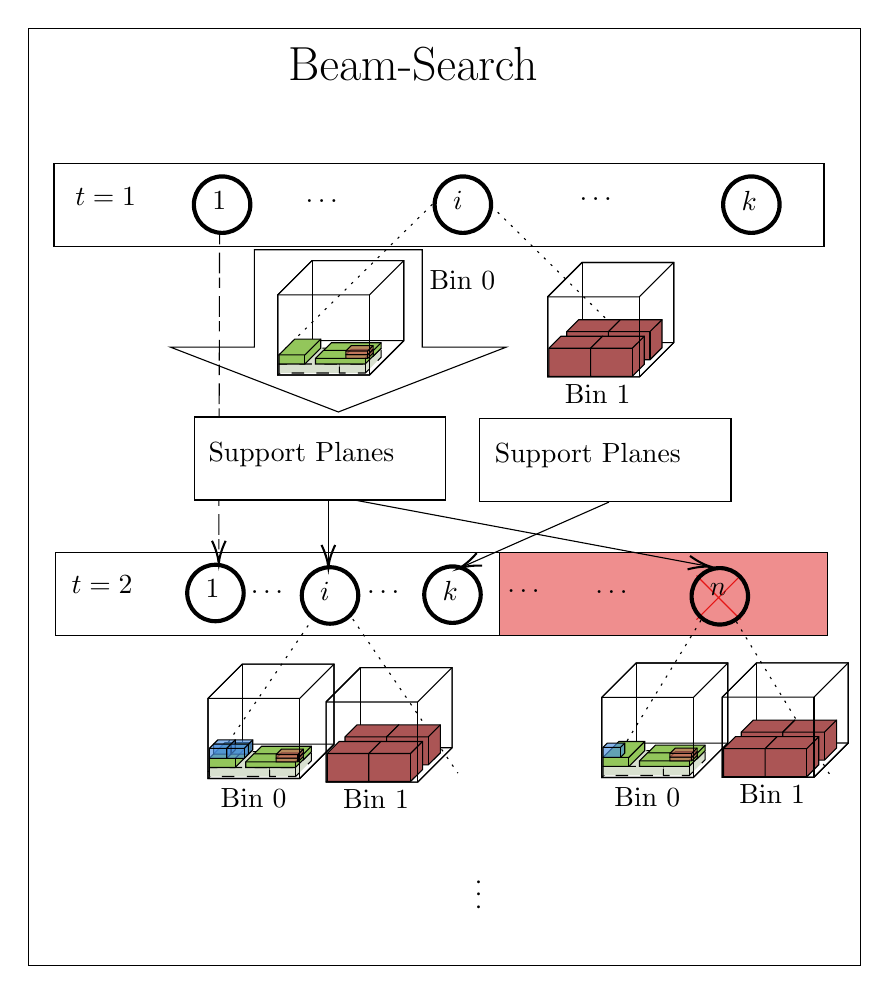
\begin{tikzpicture}[x=0.75pt,y=0.75pt,yscale=-1,xscale=1]
%uncomment if require: \path (0,540); %set diagram left start at 0, and has height of 540

%Right Arrow [id:dp8337745536636388] 
\draw   (281.86,136.75) -- (281.86,183.64) -- (322.31,183.64) -- (241.41,214.89) -- (160.5,183.64) -- (200.95,183.64) -- (200.95,136.75) -- cycle ;
%Straight Lines [id:da78157118634077] 
\draw  [dash pattern={on 3.75pt off 3pt on 7.5pt off 1.5pt}]  (184.2,129.1) -- (183.81,285.9) ;
\draw [shift={(183.8,287.9)}, rotate = 270.14] [color={rgb, 255:red, 0; green, 0; blue, 0 }  ][line width=0.75]    (10.93,-3.29) .. controls (6.95,-1.4) and (3.31,-0.3) .. (0,0) .. controls (3.31,0.3) and (6.95,1.4) .. (10.93,3.29)   ;
%Shape: Cube [id:dp22610144404804344] 
\draw   (272.94,180.54) -- (256.4,197.09) -- (212.23,197.09) -- (212.23,158.49) -- (228.77,141.94) -- (272.94,141.94) -- cycle ; \draw   (212.23,197.09) -- (228.77,180.54) -- (272.94,180.54) ; \draw   (228.77,180.54) -- (228.77,141.94) ;
%Shape: Rectangle [id:dp3675398368494672] 
\draw   (92,30) -- (493,30) -- (493,481.75) -- (92,481.75) -- cycle ;
%Shape: Rectangle [id:dp3872816319657796] 
\draw   (104.4,95) -- (475.4,95) -- (475.4,135) -- (104.4,135) -- cycle ;
%Straight Lines [id:da16266893569729468] 
\draw  [dash pattern={on 0.84pt off 2.51pt}]  (286.71,114.86) -- (211,189.14) ;
%Straight Lines [id:da2739363742069437] 
\draw  [dash pattern={on 0.84pt off 2.51pt}]  (315,115.5) -- (390.43,189.71) ;

%Shape: Cube [id:dp06723731454771065] 
\draw   (403,181.46) -- (386.46,198) -- (342.29,198) -- (342.29,159.4) -- (358.83,142.86) -- (403,142.86) -- cycle ; \draw   (342.29,198) -- (358.83,181.46) -- (403,181.46) ; \draw   (358.83,181.46) -- (358.83,142.86) ;
%Shape: Cube [id:dp9540002545180426] 
\draw  [fill={rgb, 255:red, 171; green, 85; blue, 85 }  ,fill opacity=1 ] (351.43,176.21) -- (357.21,170.43) -- (377.29,170.43) -- (377.29,183.93) -- (371.5,189.71) -- (351.43,189.71) -- cycle ; \draw   (377.29,170.43) -- (371.5,176.21) -- (351.43,176.21) ; \draw   (371.5,176.21) -- (371.5,189.71) ;
%Shape: Cube [id:dp4858900723039008] 
\draw  [fill={rgb, 255:red, 171; green, 85; blue, 85 }  ,fill opacity=1 ] (371.5,176.21) -- (377.29,170.43) -- (397.36,170.43) -- (397.36,183.93) -- (391.57,189.71) -- (371.5,189.71) -- cycle ; \draw   (397.36,170.43) -- (391.57,176.21) -- (371.5,176.21) ; \draw   (391.57,176.21) -- (391.57,189.71) ;
%Shape: Cube [id:dp37688563395090247] 
\draw  [fill={rgb, 255:red, 171; green, 85; blue, 85 }  ,fill opacity=1 ] (342.86,184.21) -- (348.64,178.43) -- (368.71,178.43) -- (368.71,191.93) -- (362.93,197.71) -- (342.86,197.71) -- cycle ; \draw   (368.71,178.43) -- (362.93,184.21) -- (342.86,184.21) ; \draw   (362.93,184.21) -- (362.93,197.71) ;
%Shape: Cube [id:dp29304074255321133] 
\draw  [fill={rgb, 255:red, 171; green, 85; blue, 85 }  ,fill opacity=1 ] (362.93,184.21) -- (368.71,178.43) -- (388.79,178.43) -- (388.79,191.93) -- (383,197.71) -- (362.93,197.71) -- cycle ; \draw   (388.79,178.43) -- (383,184.21) -- (362.93,184.21) ; \draw   (383,184.21) -- (383,197.71) ;
%Shape: Cube [id:dp012588700852047996] 
\draw   (342.29,159.4) -- (358.83,142.86) -- (403,142.86) -- (403,181.46) -- (386.46,198) -- (342.29,198) -- cycle ; \draw   (403,142.86) -- (386.46,159.4) -- (342.29,159.4) ; \draw   (386.46,159.4) -- (386.46,198) ;
%Shape: Cube [id:dp23988070590283161] 
\draw  [fill={rgb, 255:red, 216; green, 224; blue, 207 }  ,fill opacity=1 ][dash pattern={on 4.5pt off 4.5pt}] (212.84,191.76) -- (220.46,184.14) -- (249.52,184.14) -- (249.52,188.52) -- (241.9,196.13) -- (212.84,196.13) -- cycle ; \draw  [dash pattern={on 4.5pt off 4.5pt}] (249.52,184.14) -- (241.9,191.76) -- (212.84,191.76) ; \draw  [dash pattern={on 4.5pt off 4.5pt}] (241.9,191.76) -- (241.9,196.13) ;
%Shape: Cube [id:dp09035733009605551] 
\draw  [fill={rgb, 255:red, 216; green, 224; blue, 207 }  ,fill opacity=1 ][dash pattern={on 4.5pt off 4.5pt}] (241.9,191.76) -- (249.52,184.14) -- (262.04,184.14) -- (262.04,188.52) -- (254.42,196.13) -- (241.9,196.13) -- cycle ; \draw  [dash pattern={on 4.5pt off 4.5pt}] (262.04,184.14) -- (254.42,191.76) -- (241.9,191.76) ; \draw  [dash pattern={on 4.5pt off 4.5pt}] (254.42,191.76) -- (254.42,196.13) ;
%Shape: Cube [id:dp21044320148528428] 
\draw  [fill={rgb, 255:red, 147; green, 198; blue, 91 }  ,fill opacity=1 ] (212.84,187.39) -- (220.46,179.77) -- (232.93,179.77) -- (232.93,184.14) -- (225.31,191.76) -- (212.84,191.76) -- cycle ; \draw   (232.93,179.77) -- (225.31,187.39) -- (212.84,187.39) ; \draw   (225.31,187.39) -- (225.31,191.76) ;
%Shape: Cube [id:dp2634805119323166] 
\draw  [fill={rgb, 255:red, 147; green, 198; blue, 91 }  ,fill opacity=1 ] (234.29,185.34) -- (238.1,181.53) -- (262.04,181.53) -- (262.04,184.17) -- (258.22,187.99) -- (234.29,187.99) -- cycle ; \draw   (262.04,181.53) -- (258.22,185.34) -- (234.29,185.34) ; \draw   (258.22,185.34) -- (258.22,187.99) ;
%Shape: Cube [id:dp5335177162875748] 
\draw  [fill={rgb, 255:red, 147; green, 198; blue, 91 }  ,fill opacity=1 ] (230.41,189.08) -- (234.29,185.21) -- (258.16,185.21) -- (258.16,187.89) -- (254.29,191.76) -- (230.41,191.76) -- cycle ; \draw   (258.16,185.21) -- (254.29,189.08) -- (230.41,189.08) ; \draw   (254.29,189.08) -- (254.29,191.76) ;
%Shape: Cube [id:dp6236494259647203] 
\draw  [fill={rgb, 255:red, 198; green, 110; blue, 91 }  ,fill opacity=0.69 ] (245.05,187.29) -- (247.63,184.71) -- (258.16,184.71) -- (258.16,186.5) -- (255.58,189.08) -- (245.05,189.08) -- cycle ; \draw   (258.16,184.71) -- (255.58,187.29) -- (245.05,187.29) ; \draw   (255.58,187.29) -- (255.58,189.08) ;
%Shape: Cube [id:dp9516088630040508] 
\draw  [fill={rgb, 255:red, 198; green, 110; blue, 91 }  ,fill opacity=0.69 ] (245.05,185.5) -- (247.63,182.92) -- (258.16,182.92) -- (258.16,184.71) -- (255.58,187.29) -- (245.05,187.29) -- cycle ; \draw   (258.16,182.92) -- (255.58,185.5) -- (245.05,185.5) ; \draw   (255.58,185.5) -- (255.58,187.29) ;
%Shape: Cube [id:dp022246373009996434] 
\draw   (212.23,158.49) -- (228.77,141.94) -- (272.94,141.94) -- (272.94,180.54) -- (256.4,197.09) -- (212.23,197.09) -- cycle ; \draw   (272.94,141.94) -- (256.4,158.49) -- (212.23,158.49) ; \draw   (256.4,158.49) -- (256.4,197.09) ;
%Shape: Rectangle [id:dp6604290999676096] 
\draw  [fill={rgb, 255:red, 255; green, 255; blue, 255 }  ,fill opacity=1 ] (172,217.3) -- (293,217.3) -- (293,257.3) -- (172,257.3) -- cycle ;
%Shape: Rectangle [id:dp10394734829371921] 
\draw   (309.6,218.1) -- (430.6,218.1) -- (430.6,258.1) -- (309.6,258.1) -- cycle ;
%Shape: Rectangle [id:dp3884482964100383] 
\draw   (105.2,282.6) -- (476.2,282.6) -- (476.2,322.6) -- (105.2,322.6) -- cycle ;
%Shape: Rectangle [id:dp4662670618125976] 
\draw  [fill={rgb, 255:red, 239; green, 142; blue, 142 }  ,fill opacity=1 ] (319.2,282.5) -- (477,282.5) -- (477,322.5) -- (319.2,322.5) -- cycle ;
\draw  [color={rgb, 255:red, 229; green, 21; blue, 21 }  ,draw opacity=1 ] (413.99,293.69) -- (435.21,314.91)(435.21,293.69) -- (413.99,314.91) ;
%Straight Lines [id:da9423844633177114] 
\draw    (236.6,257.9) -- (236.6,287.9) ;
\draw [shift={(236.6,289.9)}, rotate = 270] [color={rgb, 255:red, 0; green, 0; blue, 0 }  ][line width=0.75]    (10.93,-3.29) .. controls (6.95,-1.4) and (3.31,-0.3) .. (0,0) .. controls (3.31,0.3) and (6.95,1.4) .. (10.93,3.29)   ;
%Straight Lines [id:da8187100513502555] 
\draw    (250.2,257.5) -- (419.03,289.13) ;
\draw [shift={(421,289.5)}, rotate = 190.61] [color={rgb, 255:red, 0; green, 0; blue, 0 }  ][line width=0.75]    (10.93,-3.29) .. controls (6.95,-1.4) and (3.31,-0.3) .. (0,0) .. controls (3.31,0.3) and (6.95,1.4) .. (10.93,3.29)   ;
%Straight Lines [id:da5112317799583161] 
\draw    (371.8,258.3) -- (301.23,289.49) ;
\draw [shift={(299.4,290.3)}, rotate = 336.16] [color={rgb, 255:red, 0; green, 0; blue, 0 }  ][line width=0.75]    (10.93,-3.29) .. controls (6.95,-1.4) and (3.31,-0.3) .. (0,0) .. controls (3.31,0.3) and (6.95,1.4) .. (10.93,3.29)   ;
%Shape: Cube [id:dp3098593802776677] 
\draw   (239.34,374.94) -- (222.8,391.49) -- (178.63,391.49) -- (178.63,352.89) -- (195.17,336.34) -- (239.34,336.34) -- cycle ; \draw   (178.63,391.49) -- (195.17,374.94) -- (239.34,374.94) ; \draw   (195.17,374.94) -- (195.17,336.34) ;
%Straight Lines [id:da052289940556063064] 
\draw  [dash pattern={on 0.84pt off 2.51pt}]  (229.41,314.06) -- (178.6,388.34) ;
%Straight Lines [id:da7979737763702788] 
\draw  [dash pattern={on 0.84pt off 2.51pt}]  (248.39,314.7) -- (299,388.91) ;

%Shape: Cube [id:dp563730868795463] 
\draw   (296.2,376.66) -- (279.66,393.2) -- (235.49,393.2) -- (235.49,354.6) -- (252.03,338.06) -- (296.2,338.06) -- cycle ; \draw   (235.49,393.2) -- (252.03,376.66) -- (296.2,376.66) ; \draw   (252.03,376.66) -- (252.03,338.06) ;
%Shape: Cube [id:dp6842297170502628] 
\draw  [fill={rgb, 255:red, 171; green, 85; blue, 85 }  ,fill opacity=1 ] (244.63,371.41) -- (250.41,365.63) -- (270.49,365.63) -- (270.49,379.13) -- (264.7,384.91) -- (244.63,384.91) -- cycle ; \draw   (270.49,365.63) -- (264.7,371.41) -- (244.63,371.41) ; \draw   (264.7,371.41) -- (264.7,384.91) ;
%Shape: Cube [id:dp36117121382423767] 
\draw  [fill={rgb, 255:red, 171; green, 85; blue, 85 }  ,fill opacity=1 ] (264.7,371.41) -- (270.49,365.63) -- (290.56,365.63) -- (290.56,379.13) -- (284.77,384.91) -- (264.7,384.91) -- cycle ; \draw   (290.56,365.63) -- (284.77,371.41) -- (264.7,371.41) ; \draw   (284.77,371.41) -- (284.77,384.91) ;
%Shape: Cube [id:dp5567622602150145] 
\draw  [fill={rgb, 255:red, 171; green, 85; blue, 85 }  ,fill opacity=1 ] (236.06,379.41) -- (241.84,373.63) -- (261.91,373.63) -- (261.91,387.13) -- (256.13,392.91) -- (236.06,392.91) -- cycle ; \draw   (261.91,373.63) -- (256.13,379.41) -- (236.06,379.41) ; \draw   (256.13,379.41) -- (256.13,392.91) ;
%Shape: Cube [id:dp9251910046018463] 
\draw  [fill={rgb, 255:red, 171; green, 85; blue, 85 }  ,fill opacity=1 ] (256.13,379.41) -- (261.91,373.63) -- (281.99,373.63) -- (281.99,387.13) -- (276.2,392.91) -- (256.13,392.91) -- cycle ; \draw   (281.99,373.63) -- (276.2,379.41) -- (256.13,379.41) ; \draw   (276.2,379.41) -- (276.2,392.91) ;
%Shape: Cube [id:dp97100963444055] 
\draw   (235.49,354.6) -- (252.03,338.06) -- (296.2,338.06) -- (296.2,376.66) -- (279.66,393.2) -- (235.49,393.2) -- cycle ; \draw   (296.2,338.06) -- (279.66,354.6) -- (235.49,354.6) ; \draw   (279.66,354.6) -- (279.66,393.2) ;
%Shape: Cube [id:dp3314229379764526] 
\draw  [fill={rgb, 255:red, 216; green, 224; blue, 207 }  ,fill opacity=1 ][dash pattern={on 4.5pt off 4.5pt}] (179.24,386.16) -- (186.86,378.54) -- (215.92,378.54) -- (215.92,382.92) -- (208.3,390.53) -- (179.24,390.53) -- cycle ; \draw  [dash pattern={on 4.5pt off 4.5pt}] (215.92,378.54) -- (208.3,386.16) -- (179.24,386.16) ; \draw  [dash pattern={on 4.5pt off 4.5pt}] (208.3,386.16) -- (208.3,390.53) ;
%Shape: Cube [id:dp4227409563137523] 
\draw  [fill={rgb, 255:red, 216; green, 224; blue, 207 }  ,fill opacity=1 ][dash pattern={on 4.5pt off 4.5pt}] (208.3,386.16) -- (215.92,378.54) -- (228.44,378.54) -- (228.44,382.92) -- (220.82,390.53) -- (208.3,390.53) -- cycle ; \draw  [dash pattern={on 4.5pt off 4.5pt}] (228.44,378.54) -- (220.82,386.16) -- (208.3,386.16) ; \draw  [dash pattern={on 4.5pt off 4.5pt}] (220.82,386.16) -- (220.82,390.53) ;
%Shape: Cube [id:dp9493780297339603] 
\draw  [fill={rgb, 255:red, 147; green, 198; blue, 91 }  ,fill opacity=1 ] (179.24,381.79) -- (186.86,374.17) -- (199.33,374.17) -- (199.33,378.54) -- (191.71,386.16) -- (179.24,386.16) -- cycle ; \draw   (199.33,374.17) -- (191.71,381.79) -- (179.24,381.79) ; \draw   (191.71,381.79) -- (191.71,386.16) ;
%Shape: Cube [id:dp20210982349003004] 
\draw  [fill={rgb, 255:red, 147; green, 198; blue, 91 }  ,fill opacity=1 ] (200.69,379.74) -- (204.5,375.93) -- (228.44,375.93) -- (228.44,378.57) -- (224.62,382.39) -- (200.69,382.39) -- cycle ; \draw   (228.44,375.93) -- (224.62,379.74) -- (200.69,379.74) ; \draw   (224.62,379.74) -- (224.62,382.39) ;
%Shape: Cube [id:dp6451220456842981] 
\draw  [fill={rgb, 255:red, 147; green, 198; blue, 91 }  ,fill opacity=1 ] (196.81,383.48) -- (200.69,379.61) -- (224.56,379.61) -- (224.56,382.29) -- (220.69,386.16) -- (196.81,386.16) -- cycle ; \draw   (224.56,379.61) -- (220.69,383.48) -- (196.81,383.48) ; \draw   (220.69,383.48) -- (220.69,386.16) ;
%Shape: Cube [id:dp3910721600427305] 
\draw  [fill={rgb, 255:red, 198; green, 110; blue, 91 }  ,fill opacity=0.69 ] (211.45,381.69) -- (214.03,379.11) -- (224.56,379.11) -- (224.56,380.9) -- (221.98,383.48) -- (211.45,383.48) -- cycle ; \draw   (224.56,379.11) -- (221.98,381.69) -- (211.45,381.69) ; \draw   (221.98,381.69) -- (221.98,383.48) ;
%Shape: Cube [id:dp23309754303051422] 
\draw  [fill={rgb, 255:red, 198; green, 110; blue, 91 }  ,fill opacity=0.69 ] (211.45,379.9) -- (214.03,377.32) -- (224.56,377.32) -- (224.56,379.11) -- (221.98,381.69) -- (211.45,381.69) -- cycle ; \draw   (224.56,377.32) -- (221.98,379.9) -- (211.45,379.9) ; \draw   (221.98,379.9) -- (221.98,381.69) ;
%Shape: Cube [id:dp4655482842473665] 
\draw   (178.63,352.89) -- (195.17,336.34) -- (239.34,336.34) -- (239.34,374.94) -- (222.8,391.49) -- (178.63,391.49) -- cycle ; \draw   (239.34,336.34) -- (222.8,352.89) -- (178.63,352.89) ; \draw   (222.8,352.89) -- (222.8,391.49) ;
%Shape: Cube [id:dp4152358812705026] 
\draw   (429.04,374.44) -- (412.5,390.99) -- (368.33,390.99) -- (368.33,352.39) -- (384.87,335.84) -- (429.04,335.84) -- cycle ; \draw   (368.33,390.99) -- (384.87,374.44) -- (429.04,374.44) ; \draw   (384.87,374.44) -- (384.87,335.84) ;
%Straight Lines [id:da6929539156017857] 
\draw  [dash pattern={on 0.84pt off 2.51pt}]  (416.13,315.26) -- (370.6,389.54) ;
%Straight Lines [id:da2520104054773419] 
\draw  [dash pattern={on 0.84pt off 2.51pt}]  (433.14,315.9) -- (478.5,390.11) ;

%Shape: Cube [id:dp30742448269234246] 
\draw   (487.1,374.36) -- (470.56,390.9) -- (426.39,390.9) -- (426.39,352.3) -- (442.93,335.76) -- (487.1,335.76) -- cycle ; \draw   (426.39,390.9) -- (442.93,374.36) -- (487.1,374.36) ; \draw   (442.93,374.36) -- (442.93,335.76) ;
%Shape: Cube [id:dp5547181392678717] 
\draw  [fill={rgb, 255:red, 171; green, 85; blue, 85 }  ,fill opacity=1 ] (435.53,369.11) -- (441.31,363.33) -- (461.39,363.33) -- (461.39,376.83) -- (455.6,382.61) -- (435.53,382.61) -- cycle ; \draw   (461.39,363.33) -- (455.6,369.11) -- (435.53,369.11) ; \draw   (455.6,369.11) -- (455.6,382.61) ;
%Shape: Cube [id:dp7714989563411607] 
\draw  [fill={rgb, 255:red, 171; green, 85; blue, 85 }  ,fill opacity=1 ] (455.6,369.11) -- (461.39,363.33) -- (481.46,363.33) -- (481.46,376.83) -- (475.67,382.61) -- (455.6,382.61) -- cycle ; \draw   (481.46,363.33) -- (475.67,369.11) -- (455.6,369.11) ; \draw   (475.67,369.11) -- (475.67,382.61) ;
%Shape: Cube [id:dp6802562603958051] 
\draw  [fill={rgb, 255:red, 171; green, 85; blue, 85 }  ,fill opacity=1 ] (426.96,377.11) -- (432.74,371.33) -- (452.81,371.33) -- (452.81,384.83) -- (447.03,390.61) -- (426.96,390.61) -- cycle ; \draw   (452.81,371.33) -- (447.03,377.11) -- (426.96,377.11) ; \draw   (447.03,377.11) -- (447.03,390.61) ;
%Shape: Cube [id:dp3575223135416413] 
\draw  [fill={rgb, 255:red, 171; green, 85; blue, 85 }  ,fill opacity=1 ] (447.03,377.11) -- (452.81,371.33) -- (472.89,371.33) -- (472.89,384.83) -- (467.1,390.61) -- (447.03,390.61) -- cycle ; \draw   (472.89,371.33) -- (467.1,377.11) -- (447.03,377.11) ; \draw   (467.1,377.11) -- (467.1,390.61) ;
%Shape: Cube [id:dp04583492087348129] 
\draw   (426.39,352.3) -- (442.93,335.76) -- (487.1,335.76) -- (487.1,374.36) -- (470.56,390.9) -- (426.39,390.9) -- cycle ; \draw   (487.1,335.76) -- (470.56,352.3) -- (426.39,352.3) ; \draw   (470.56,352.3) -- (470.56,390.9) ;
%Shape: Cube [id:dp22648598314600765] 
\draw  [fill={rgb, 255:red, 216; green, 224; blue, 207 }  ,fill opacity=1 ][dash pattern={on 4.5pt off 4.5pt}] (368.94,385.66) -- (376.56,378.04) -- (405.62,378.04) -- (405.62,382.42) -- (398,390.03) -- (368.94,390.03) -- cycle ; \draw  [dash pattern={on 4.5pt off 4.5pt}] (405.62,378.04) -- (398,385.66) -- (368.94,385.66) ; \draw  [dash pattern={on 4.5pt off 4.5pt}] (398,385.66) -- (398,390.03) ;
%Shape: Cube [id:dp11910803660750402] 
\draw  [fill={rgb, 255:red, 216; green, 224; blue, 207 }  ,fill opacity=1 ][dash pattern={on 4.5pt off 4.5pt}] (398,385.66) -- (405.62,378.04) -- (418.14,378.04) -- (418.14,382.42) -- (410.52,390.03) -- (398,390.03) -- cycle ; \draw  [dash pattern={on 4.5pt off 4.5pt}] (418.14,378.04) -- (410.52,385.66) -- (398,385.66) ; \draw  [dash pattern={on 4.5pt off 4.5pt}] (410.52,385.66) -- (410.52,390.03) ;
%Shape: Cube [id:dp03436669328315789] 
\draw  [fill={rgb, 255:red, 147; green, 198; blue, 91 }  ,fill opacity=1 ] (368.94,381.29) -- (376.56,373.67) -- (389.03,373.67) -- (389.03,378.04) -- (381.41,385.66) -- (368.94,385.66) -- cycle ; \draw   (389.03,373.67) -- (381.41,381.29) -- (368.94,381.29) ; \draw   (381.41,381.29) -- (381.41,385.66) ;
%Shape: Cube [id:dp3001366964737242] 
\draw  [fill={rgb, 255:red, 147; green, 198; blue, 91 }  ,fill opacity=1 ] (390.39,379.24) -- (394.2,375.43) -- (418.14,375.43) -- (418.14,378.07) -- (414.32,381.89) -- (390.39,381.89) -- cycle ; \draw   (418.14,375.43) -- (414.32,379.24) -- (390.39,379.24) ; \draw   (414.32,379.24) -- (414.32,381.89) ;
%Shape: Cube [id:dp9791091368910745] 
\draw  [fill={rgb, 255:red, 147; green, 198; blue, 91 }  ,fill opacity=1 ] (386.51,382.98) -- (390.39,379.11) -- (414.26,379.11) -- (414.26,381.79) -- (410.39,385.66) -- (386.51,385.66) -- cycle ; \draw   (414.26,379.11) -- (410.39,382.98) -- (386.51,382.98) ; \draw   (410.39,382.98) -- (410.39,385.66) ;
%Shape: Cube [id:dp5345838256134253] 
\draw  [fill={rgb, 255:red, 198; green, 110; blue, 91 }  ,fill opacity=0.69 ] (401.15,381.19) -- (403.73,378.61) -- (414.26,378.61) -- (414.26,380.4) -- (411.68,382.98) -- (401.15,382.98) -- cycle ; \draw   (414.26,378.61) -- (411.68,381.19) -- (401.15,381.19) ; \draw   (411.68,381.19) -- (411.68,382.98) ;
%Shape: Cube [id:dp8233627388074675] 
\draw  [fill={rgb, 255:red, 74; green, 144; blue, 226 }  ,fill opacity=0.66 ] (368.94,376.49) -- (370.99,374.44) -- (379.4,374.44) -- (379.4,379.24) -- (377.34,381.29) -- (368.94,381.29) -- cycle ; \draw   (379.4,374.44) -- (377.34,376.49) -- (368.94,376.49) ; \draw   (377.34,376.49) -- (377.34,381.29) ;
%Shape: Cube [id:dp3945702568476691] 
\draw  [fill={rgb, 255:red, 198; green, 110; blue, 91 }  ,fill opacity=0.69 ] (401.15,379.4) -- (403.73,376.82) -- (414.26,376.82) -- (414.26,378.61) -- (411.68,381.19) -- (401.15,381.19) -- cycle ; \draw   (414.26,376.82) -- (411.68,379.4) -- (401.15,379.4) ; \draw   (411.68,379.4) -- (411.68,381.19) ;
%Shape: Cube [id:dp8251331839204266] 
\draw   (368.33,352.39) -- (384.87,335.84) -- (429.04,335.84) -- (429.04,374.44) -- (412.5,390.99) -- (368.33,390.99) -- cycle ; \draw   (429.04,335.84) -- (412.5,352.39) -- (368.33,352.39) ; \draw   (412.5,352.39) -- (412.5,390.99) ;
%Shape: Cube [id:dp2708464120930435] 
\draw  [fill={rgb, 255:red, 74; green, 144; blue, 226 }  ,fill opacity=0.66 ] (189.7,374.94) -- (191.75,372.88) -- (200.16,372.88) -- (200.16,377.68) -- (198.1,379.74) -- (189.7,379.74) -- cycle ; \draw   (200.16,372.88) -- (198.1,374.94) -- (189.7,374.94) ; \draw   (198.1,374.94) -- (198.1,379.74) ;
%Shape: Cube [id:dp15483932168959624] 
\draw  [fill={rgb, 255:red, 74; green, 144; blue, 226 }  ,fill opacity=0.66 ] (181.29,374.94) -- (183.35,372.88) -- (191.75,372.88) -- (191.75,377.68) -- (189.7,379.74) -- (181.29,379.74) -- cycle ; \draw   (191.75,372.88) -- (189.7,374.94) -- (181.29,374.94) ; \draw   (189.7,374.94) -- (189.7,379.74) ;
%Shape: Cube [id:dp5792684196727304] 
\draw  [fill={rgb, 255:red, 74; green, 144; blue, 226 }  ,fill opacity=0.66 ] (179.24,376.99) -- (181.29,374.94) -- (189.7,374.94) -- (189.7,379.74) -- (187.64,381.79) -- (179.24,381.79) -- cycle ; \draw   (189.7,374.94) -- (187.64,376.99) -- (179.24,376.99) ; \draw   (187.64,376.99) -- (187.64,381.79) ;
%Shape: Cube [id:dp6982160774307449] 
\draw  [fill={rgb, 255:red, 74; green, 144; blue, 226 }  ,fill opacity=0.66 ] (187.64,376.99) -- (189.7,374.94) -- (198.1,374.94) -- (198.1,379.74) -- (196.04,381.79) -- (187.64,381.79) -- cycle ; \draw   (198.1,374.94) -- (196.04,376.99) -- (187.64,376.99) ; \draw   (196.04,376.99) -- (196.04,381.79) ;

% Text Node
\draw (216,38) node [anchor=north west][inner sep=0.75pt]   [align=left] {{\LARGE Beam-Search}};
% Text Node
\draw  [line width=1.5]   (185.4, 115) circle [x radius= 13.6, y radius= 13.6]   ;
\draw (179.4,107.4) node [anchor=north west][inner sep=0.75pt]    {$1$};
% Text Node
\draw (113.4,105.4) node [anchor=north west][inner sep=0.75pt]    {$t=1$};
% Text Node
\draw  [line width=1.5]   (301.4, 115) circle [x radius= 13.6, y radius= 13.6]   ;
\draw (295.4,107.4) node [anchor=north west][inner sep=0.75pt]    {$i$};
% Text Node
\draw  [line width=1.5]   (440.4, 115) circle [x radius= 13.6, y radius= 13.6]   ;
\draw (434.4,107.4) node [anchor=north west][inner sep=0.75pt]    {$k$};
% Text Node
\draw (224.4,111.4) node [anchor=north west][inner sep=0.75pt]    {$\dotsc $};
% Text Node
\draw (356.4,110.4) node [anchor=north west][inner sep=0.75pt]    {$\dotsc $};
% Text Node
\draw (284.09,145.3) node [anchor=north west][inner sep=0.75pt]   [align=left] {Bin 0};
% Text Node
\draw (349.26,200.23) node [anchor=north west][inner sep=0.75pt]   [align=left] {Bin 1};
% Text Node
\draw (177.6,228.1) node [anchor=north west][inner sep=0.75pt]   [align=left] {Support Planes};
% Text Node
\draw (315.6,228.5) node [anchor=north west][inner sep=0.75pt]   [align=left] {Support Planes};
% Text Node
\draw  [line width=1.5]   (182.2, 302.1) circle [x radius= 13.6, y radius= 13.6]   ;
\draw (176.2,294.5) node [anchor=north west][inner sep=0.75pt]    {$1$};
% Text Node
\draw (111.7,292.5) node [anchor=north west][inner sep=0.75pt]    {$t=2$};
% Text Node
\draw  [line width=1.5]   (237.4, 303.3) circle [x radius= 13.6, y radius= 13.6]   ;
\draw (231.4,295.7) node [anchor=north west][inner sep=0.75pt]    {$i$};
% Text Node
\draw  [line width=1.5]   (296.4, 302.9) circle [x radius= 13.6, y radius= 13.6]   ;
\draw (290.4,295.3) node [anchor=north west][inner sep=0.75pt]    {$k$};
% Text Node
\draw (198,299.7) node [anchor=north west][inner sep=0.75pt]    {$\dotsc $};
% Text Node
\draw (254,299.5) node [anchor=north west][inner sep=0.75pt]    {$\dotsc $};
% Text Node
\draw (321.6,299.1) node [anchor=north west][inner sep=0.75pt]    {$\dotsc $};
% Text Node
\draw  [line width=1.5]   (425.2, 303.7) circle [x radius= 13.6, y radius= 13.6]   ;
\draw (419.2,296.1) node [anchor=north west][inner sep=0.75pt]    {$n$};
% Text Node
\draw (364,299.5) node [anchor=north west][inner sep=0.75pt]    {$\dotsc $};
% Text Node
\draw (310.95,438.37) node [anchor=north west][inner sep=0.75pt]  [rotate=-89.78]  {$\dotsc $};
% Text Node
\draw (183.49,395.2) node [anchor=north west][inner sep=0.75pt]   [align=left] {Bin 0};
% Text Node
\draw (242.46,395.43) node [anchor=north west][inner sep=0.75pt]   [align=left] {Bin 1};
% Text Node
\draw (373.19,394.7) node [anchor=north west][inner sep=0.75pt]   [align=left] {Bin 0};
% Text Node
\draw (433.36,393.13) node [anchor=north west][inner sep=0.75pt]   [align=left] {Bin 1};


\end{tikzpicture}

                }
                \caption{Conceptual representation of the proposed heuristic}
                \label{fig:heur_scheme}
            \end{figure}
        \end{columns}
    \end{frame}
    \begin{frame}{Support Planes}
        \begin{columns}[onlytextwidth,T]
            \column{\dimexpr\linewidth-65mm-5mm}
            \begin{itemize}
                \item Operates on a single bin
                \item Items generate planes
                \item Planes have obstacles or support items
                \item Insertions on the lowest possible planes
                \item Exploits a modified 2D-BPP heuristic
                \item No explicit layers
            \end{itemize}
            \column{65mm}
                \begin{figure}[h]
                    \resizebox*{\columnwidth}{!}{%
                    

\tikzset{every picture/.style={line width=0.75pt}} %set default line width to 0.75pt        

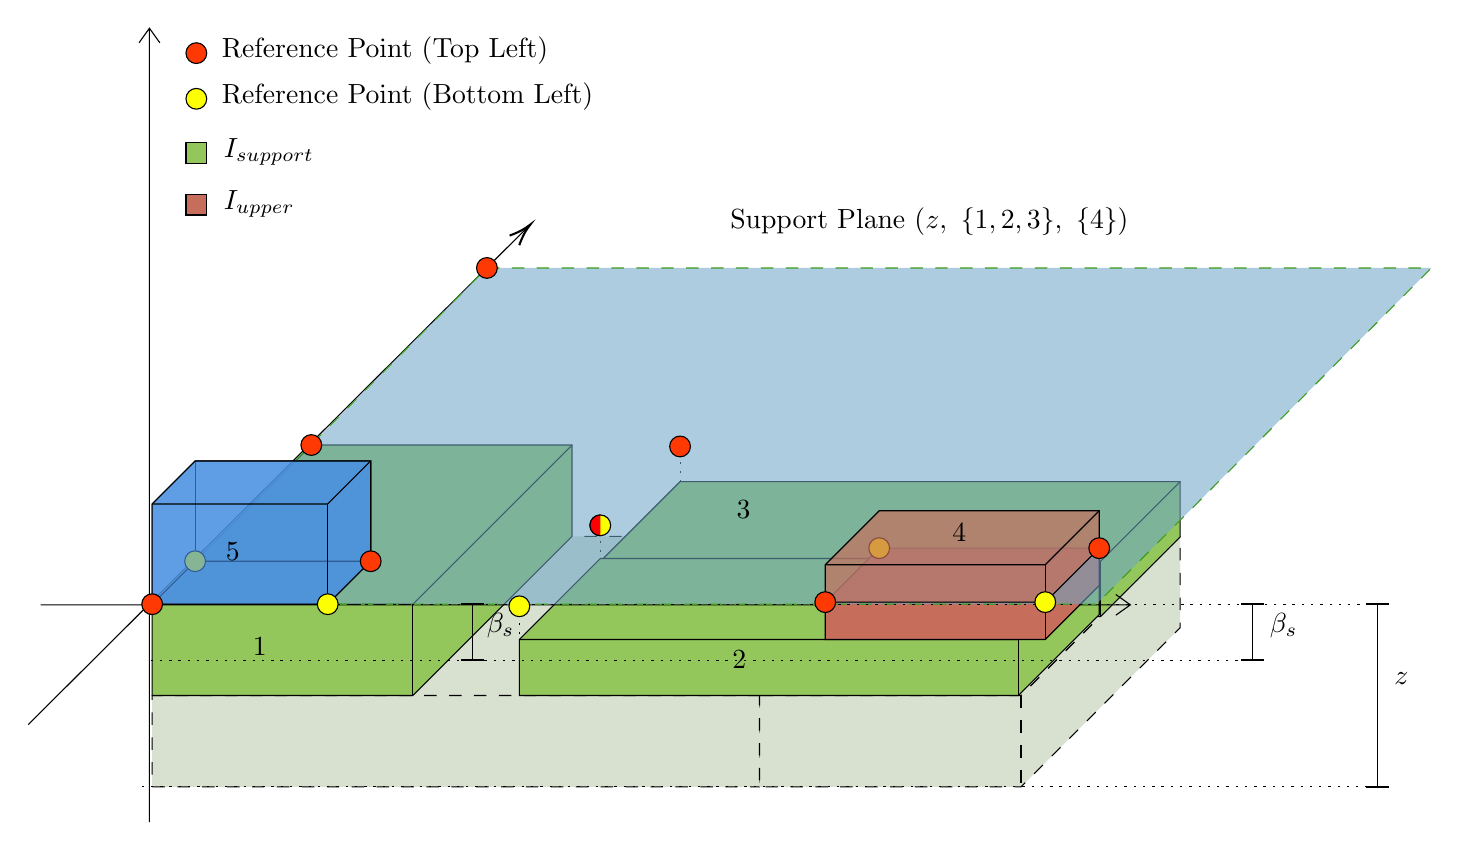
\begin{tikzpicture}[x=0.75pt,y=0.75pt,yscale=-1,xscale=1]
%uncomment if require: \path (0,412); %set diagram left start at 0, and has height of 412

%Shape: Cube [id:dp7106500856615827] 
\draw  [fill={rgb, 255:red, 216; green, 224; blue, 207 }  ,fill opacity=1 ][dash pattern={on 4.5pt off 4.5pt}] (69.7,334.5) -- (146.4,257.81) -- (439,257.81) -- (439,301.81) -- (362.31,378.5) -- (69.7,378.5) -- cycle ; \draw  [dash pattern={on 4.5pt off 4.5pt}] (439,257.81) -- (362.31,334.5) -- (69.7,334.5) ; \draw  [dash pattern={on 4.5pt off 4.5pt}] (362.31,334.5) -- (362.31,378.5) ;
%Straight Lines [id:da8316956251676535] 
\draw  [dash pattern={on 0.84pt off 2.51pt}]  (285.62,269.89) -- (285.62,252.5) ;
%Straight Lines [id:da38384433092333237] 
\draw  [dash pattern={on 0.84pt off 2.51pt}]  (324.05,231.89) -- (324.05,214.5) ;
%Shape: Cube [id:dp47709739603214574] 
\draw  [fill={rgb, 255:red, 216; green, 224; blue, 207 }  ,fill opacity=1 ][dash pattern={on 4.5pt off 4.5pt}] (362.31,334.5) -- (439,257.81) -- (565,257.81) -- (565,301.81) -- (488.31,378.5) -- (362.31,378.5) -- cycle ; \draw  [dash pattern={on 4.5pt off 4.5pt}] (565,257.81) -- (488.31,334.5) -- (362.31,334.5) ; \draw  [dash pattern={on 4.5pt off 4.5pt}] (488.31,334.5) -- (488.31,378.5) ;
%Shape: Cube [id:dp7977002200403227] 
\draw  [fill={rgb, 255:red, 147; green, 198; blue, 91 }  ,fill opacity=1 ] (69.7,290.5) -- (146.4,213.81) -- (272,213.81) -- (272,257.81) -- (195.31,334.5) -- (69.7,334.5) -- cycle ; \draw   (272,213.81) -- (195.31,290.5) -- (69.7,290.5) ; \draw   (195.31,290.5) -- (195.31,334.5) ;
%Shape: Cube [id:dp7121611670665484] 
\draw  [fill={rgb, 255:red, 147; green, 198; blue, 91 }  ,fill opacity=1 ] (285.62,269.89) -- (324.05,231.46) -- (565,231.46) -- (565,258.06) -- (526.56,296.5) -- (285.62,296.5) -- cycle ; \draw   (565,231.46) -- (526.56,269.89) -- (285.62,269.89) ; \draw   (526.56,269.89) -- (526.56,296.5) ;
%Shape: Cube [id:dp604763542929154] 
\draw  [fill={rgb, 255:red, 147; green, 198; blue, 91 }  ,fill opacity=1 ] (246.62,307.5) -- (285.62,268.5) -- (526,268.5) -- (526,295.5) -- (487,334.5) -- (246.62,334.5) -- cycle ; \draw   (526,268.5) -- (487,307.5) -- (246.62,307.5) ; \draw   (487,307.5) -- (487,334.5) ;
%Shape: Axis 2D [id:dp786981943451631] 
\draw  (16,290.81) -- (541,290.81)(68.4,13) -- (68.4,395.5) (534,285.81) -- (541,290.81) -- (534,295.81) (63.4,20) -- (68.4,13) -- (73.4,20)  ;
%Straight Lines [id:da31524103851047525] 
\draw    (10,348.5) -- (250.58,108.91) ;
\draw [shift={(252,107.5)}, rotate = 135.12] [color={rgb, 255:red, 0; green, 0; blue, 0 }  ][line width=0.75]    (10.93,-3.29) .. controls (6.95,-1.4) and (3.31,-0.3) .. (0,0) .. controls (3.31,0.3) and (6.95,1.4) .. (10.93,3.29)   ;
%Shape: Cube [id:dp6424617162036526] 
\draw  [fill={rgb, 255:red, 198; green, 110; blue, 91 }  ,fill opacity=1 ] (394,289.5) -- (420,263.5) -- (526,263.5) -- (526,281.5) -- (500,307.5) -- (394,307.5) -- cycle ; \draw   (526,263.5) -- (500,289.5) -- (394,289.5) ; \draw   (500,289.5) -- (500,307.5) ;
%Shape: Parallelogram [id:dp3639839698249763] 
\draw  [color={rgb, 255:red, 62; green, 156; blue, 30 }  ,draw opacity=1 ][fill={rgb, 255:red, 110; green, 165; blue, 200 }  ,fill opacity=0.57 ][dash pattern={on 4.5pt off 4.5pt}] (231,128.5) -- (686,128.5) -- (524.7,290.5) -- (69.7,290.5) -- cycle ;
%Straight Lines [id:da11997650250706615] 
\draw    (659.96,290.5) -- (659.96,378.5) ;
\draw [shift={(659.96,378.5)}, rotate = 270] [color={rgb, 255:red, 0; green, 0; blue, 0 }  ][line width=0.75]    (0,5.59) -- (0,-5.59)   ;
\draw [shift={(659.96,290.5)}, rotate = 270] [color={rgb, 255:red, 0; green, 0; blue, 0 }  ][line width=0.75]    (0,5.59) -- (0,-5.59)   ;
%Straight Lines [id:da7479086158615895] 
\draw  [dash pattern={on 0.84pt off 2.51pt}]  (69.7,290.5) -- (665,290.5) ;
%Straight Lines [id:da00936893511639092] 
\draw  [dash pattern={on 0.84pt off 2.51pt}]  (64.66,378.5) -- (659.96,378.5) ;
%Straight Lines [id:da2603505755036556] 
\draw  [dash pattern={on 0.84pt off 2.51pt}]  (69,317.5) -- (600,317.5) ;
%Straight Lines [id:da21695403696781168] 
\draw    (600,290.5) -- (600,317.5) ;
\draw [shift={(600,317.5)}, rotate = 270] [color={rgb, 255:red, 0; green, 0; blue, 0 }  ][line width=0.75]    (0,5.59) -- (0,-5.59)   ;
\draw [shift={(600,290.5)}, rotate = 270] [color={rgb, 255:red, 0; green, 0; blue, 0 }  ][line width=0.75]    (0,5.59) -- (0,-5.59)   ;
%Straight Lines [id:da17628222853988207] 
\draw    (224,290.5) -- (224,317.5) ;
\draw [shift={(224,317.5)}, rotate = 270] [color={rgb, 255:red, 0; green, 0; blue, 0 }  ][line width=0.75]    (0,5.59) -- (0,-5.59)   ;
\draw [shift={(224,290.5)}, rotate = 270] [color={rgb, 255:red, 0; green, 0; blue, 0 }  ][line width=0.75]    (0,5.59) -- (0,-5.59)   ;
%Shape: Cube [id:dp458320338188952] 
\draw  [fill={rgb, 255:red, 74; green, 144; blue, 226 }  ,fill opacity=0.66 ] (175,269.8) -- (154.3,290.5) -- (69.7,290.5) -- (69.7,242.2) -- (90.4,221.5) -- (175,221.5) -- cycle ; \draw   (69.7,290.5) -- (90.4,269.8) -- (175,269.8) ; \draw   (90.4,269.8) -- (90.4,221.5) ;
%Shape: Circle [id:dp9728798663710179] 
\draw  [fill={rgb, 255:red, 252; green, 255; blue, 4 }  ,fill opacity=1 ] (86,47) .. controls (86,44.24) and (88.24,42) .. (91,42) .. controls (93.76,42) and (96,44.24) .. (96,47) .. controls (96,49.76) and (93.76,52) .. (91,52) .. controls (88.24,52) and (86,49.76) .. (86,47) -- cycle ;
%Shape: Circle [id:dp41733873180988235] 
\draw  [fill={rgb, 255:red, 252; green, 255; blue, 4 }  ,fill opacity=1 ] (85.4,269.8) .. controls (85.4,267.04) and (87.64,264.8) .. (90.4,264.8) .. controls (93.17,264.8) and (95.4,267.04) .. (95.4,269.8) .. controls (95.4,272.56) and (93.17,274.8) .. (90.4,274.8) .. controls (87.64,274.8) and (85.4,272.56) .. (85.4,269.8) -- cycle ;
%Shape: Cube [id:dp9609158816144449] 
\draw  [fill={rgb, 255:red, 74; green, 144; blue, 226 }  ,fill opacity=0.66 ] (69.7,242.2) -- (90.4,221.5) -- (175,221.5) -- (175,269.8) -- (154.3,290.5) -- (69.7,290.5) -- cycle ; \draw   (175,221.5) -- (154.3,242.2) -- (69.7,242.2) ; \draw   (154.3,242.2) -- (154.3,290.5) ;
%Shape: Circle [id:dp7069570068237806] 
\draw  [fill={rgb, 255:red, 252; green, 255; blue, 4 }  ,fill opacity=1 ] (149.3,290.5) .. controls (149.3,287.74) and (151.54,285.5) .. (154.3,285.5) .. controls (157.06,285.5) and (159.3,287.74) .. (159.3,290.5) .. controls (159.3,293.26) and (157.06,295.5) .. (154.3,295.5) .. controls (151.54,295.5) and (149.3,293.26) .. (149.3,290.5) -- cycle ;
%Shape: Circle [id:dp07493756825553233] 
\draw  [fill={rgb, 255:red, 252; green, 255; blue, 4 }  ,fill opacity=1 ] (241.62,291.5) .. controls (241.62,288.74) and (243.86,286.5) .. (246.62,286.5) .. controls (249.38,286.5) and (251.62,288.74) .. (251.62,291.5) .. controls (251.62,294.26) and (249.38,296.5) .. (246.62,296.5) .. controls (243.86,296.5) and (241.62,294.26) .. (241.62,291.5) -- cycle ;
%Shape: Circle [id:dp9652867077591403] 
\draw  [fill={rgb, 255:red, 252; green, 255; blue, 4 }  ,fill opacity=1 ] (280.62,252.5) .. controls (280.62,249.74) and (282.86,247.5) .. (285.62,247.5) .. controls (288.38,247.5) and (290.62,249.74) .. (290.62,252.5) .. controls (290.62,255.26) and (288.38,257.5) .. (285.62,257.5) .. controls (282.86,257.5) and (280.62,255.26) .. (280.62,252.5) -- cycle ;
%Straight Lines [id:da7143423337159592] 
\draw  [dash pattern={on 0.84pt off 2.51pt}]  (246.62,313.89) -- (246.62,296.5) ;
%Shape: Rectangle [id:dp672375593139905] 
\draw  [fill={rgb, 255:red, 147; green, 198; blue, 91 }  ,fill opacity=1 ] (86,68) -- (96,68) -- (96,78) -- (86,78) -- cycle ;
%Shape: Rectangle [id:dp16133242915286994] 
\draw  [fill={rgb, 255:red, 198; green, 110; blue, 91 }  ,fill opacity=1 ] (86,93) -- (96,93) -- (96,103) -- (86,103) -- cycle ;
%Shape: Circle [id:dp7335317400317659] 
\draw  [fill={rgb, 255:red, 255; green, 57; blue, 4 }  ,fill opacity=1 ] (86,25) .. controls (86,22.24) and (88.24,20) .. (91,20) .. controls (93.76,20) and (96,22.24) .. (96,25) .. controls (96,27.76) and (93.76,30) .. (91,30) .. controls (88.24,30) and (86,27.76) .. (86,25) -- cycle ;
%Shape: Circle [id:dp4790782266696906] 
\draw  [fill={rgb, 255:red, 255; green, 57; blue, 4 }  ,fill opacity=1 ] (319.05,214.5) .. controls (319.05,211.74) and (321.29,209.5) .. (324.05,209.5) .. controls (326.82,209.5) and (329.05,211.74) .. (329.05,214.5) .. controls (329.05,217.26) and (326.82,219.5) .. (324.05,219.5) .. controls (321.29,219.5) and (319.05,217.26) .. (319.05,214.5) -- cycle ;
%Shape: Circle [id:dp3675058769915285] 
\draw  [fill={rgb, 255:red, 255; green, 57; blue, 4 }  ,fill opacity=1 ] (141.4,213.81) .. controls (141.4,211.05) and (143.63,208.81) .. (146.4,208.81) .. controls (149.16,208.81) and (151.4,211.05) .. (151.4,213.81) .. controls (151.4,216.57) and (149.16,218.81) .. (146.4,218.81) .. controls (143.63,218.81) and (141.4,216.57) .. (141.4,213.81) -- cycle ;
%Shape: Circle [id:dp6836568323907531] 
\draw  [fill={rgb, 255:red, 255; green, 57; blue, 4 }  ,fill opacity=1 ] (170,269.8) .. controls (170,267.04) and (172.24,264.8) .. (175,264.8) .. controls (177.76,264.8) and (180,267.04) .. (180,269.8) .. controls (180,272.56) and (177.76,274.8) .. (175,274.8) .. controls (172.24,274.8) and (170,272.56) .. (170,269.8) -- cycle ;
%Shape: Circle [id:dp9319287698621804] 
\draw  [fill={rgb, 255:red, 255; green, 57; blue, 4 }  ,fill opacity=1 ] (64.7,290.5) .. controls (64.7,287.74) and (66.94,285.5) .. (69.7,285.5) .. controls (72.47,285.5) and (74.7,287.74) .. (74.7,290.5) .. controls (74.7,293.26) and (72.47,295.5) .. (69.7,295.5) .. controls (66.94,295.5) and (64.7,293.26) .. (64.7,290.5) -- cycle ;
%Shape: Arc [id:dp7222867806291037] 
\draw  [draw opacity=0][fill={rgb, 255:red, 251; green, 1; blue, 1 }  ,fill opacity=1 ] (285.62,257.5) .. controls (285.62,257.5) and (285.62,257.5) .. (285.62,257.5) .. controls (285.62,257.5) and (285.62,257.5) .. (285.62,257.5) .. controls (282.86,257.5) and (280.62,255.26) .. (280.62,252.5) .. controls (280.62,249.74) and (282.86,247.5) .. (285.62,247.5) -- (285.62,252.5) -- cycle ; \draw   (285.62,257.5) .. controls (285.62,257.5) and (285.62,257.5) .. (285.62,257.5) .. controls (285.62,257.5) and (285.62,257.5) .. (285.62,257.5) .. controls (282.86,257.5) and (280.62,255.26) .. (280.62,252.5) .. controls (280.62,249.74) and (282.86,247.5) .. (285.62,247.5) ;  
%Shape: Circle [id:dp7431470261343242] 
\draw  [fill={rgb, 255:red, 252; green, 255; blue, 4 }  ,fill opacity=1 ] (415,263.5) .. controls (415,260.74) and (417.24,258.5) .. (420,258.5) .. controls (422.76,258.5) and (425,260.74) .. (425,263.5) .. controls (425,266.26) and (422.76,268.5) .. (420,268.5) .. controls (417.24,268.5) and (415,266.26) .. (415,263.5) -- cycle ;
%Shape: Cube [id:dp46874066075395426] 
\draw  [fill={rgb, 255:red, 198; green, 110; blue, 91 }  ,fill opacity=0.69 ] (394,271.5) -- (420,245.5) -- (526,245.5) -- (526,263.5) -- (500,289.5) -- (394,289.5) -- cycle ; \draw   (526,245.5) -- (500,271.5) -- (394,271.5) ; \draw   (500,271.5) -- (500,289.5) ;
%Shape: Circle [id:dp4546060900911436] 
\draw  [fill={rgb, 255:red, 252; green, 255; blue, 4 }  ,fill opacity=1 ] (495,289.5) .. controls (495,286.74) and (497.24,284.5) .. (500,284.5) .. controls (502.76,284.5) and (505,286.74) .. (505,289.5) .. controls (505,292.26) and (502.76,294.5) .. (500,294.5) .. controls (497.24,294.5) and (495,292.26) .. (495,289.5) -- cycle ;
%Shape: Circle [id:dp1099531157368071] 
\draw  [fill={rgb, 255:red, 255; green, 57; blue, 4 }  ,fill opacity=1 ] (521,263.5) .. controls (521,260.74) and (523.24,258.5) .. (526,258.5) .. controls (528.76,258.5) and (531,260.74) .. (531,263.5) .. controls (531,266.26) and (528.76,268.5) .. (526,268.5) .. controls (523.24,268.5) and (521,266.26) .. (521,263.5) -- cycle ;
%Shape: Circle [id:dp6477599340697807] 
\draw  [fill={rgb, 255:red, 255; green, 57; blue, 4 }  ,fill opacity=1 ] (389,289.5) .. controls (389,286.74) and (391.24,284.5) .. (394,284.5) .. controls (396.76,284.5) and (399,286.74) .. (399,289.5) .. controls (399,292.26) and (396.76,294.5) .. (394,294.5) .. controls (391.24,294.5) and (389,292.26) .. (389,289.5) -- cycle ;
%Shape: Circle [id:dp38665130344221843] 
\draw  [fill={rgb, 255:red, 255; green, 57; blue, 4 }  ,fill opacity=1 ] (226,128.5) .. controls (226,125.74) and (228.24,123.5) .. (231,123.5) .. controls (233.76,123.5) and (236,125.74) .. (236,128.5) .. controls (236,131.26) and (233.76,133.5) .. (231,133.5) .. controls (228.24,133.5) and (226,131.26) .. (226,128.5) -- cycle ;

% Text Node
\draw (667,322.4) node [anchor=north west][inner sep=0.75pt]    {$z$};
% Text Node
\draw (347,98) node [anchor=north west][inner sep=0.75pt]   [align=left] {Support Plane $\displaystyle ( z,\ \{1,2,3\} ,\ \{4\})$};
% Text Node
\draw (104,259.4) node [anchor=north west][inner sep=0.75pt]    {$5$};
% Text Node
\draw (117,305.4) node [anchor=north west][inner sep=0.75pt]    {$1$};
% Text Node
\draw (348,311.4) node [anchor=north west][inner sep=0.75pt]    {$2$};
% Text Node
\draw (350,239.4) node [anchor=north west][inner sep=0.75pt]    {$3$};
% Text Node
\draw (454,250.4) node [anchor=north west][inner sep=0.75pt]    {$4$};
% Text Node
\draw (607,293.4) node [anchor=north west][inner sep=0.75pt]    {$\beta _{s}$};
% Text Node
\draw (229.67,293.4) node [anchor=north west][inner sep=0.75pt]    {$\beta _{s}$};
% Text Node
\draw (102,38) node [anchor=north west][inner sep=0.75pt]   [align=left] {Reference Point (Bottom Left)};
% Text Node
\draw (103,65) node [anchor=north west][inner sep=0.75pt]   [align=left] {$\displaystyle I_{support}$};
% Text Node
\draw (103,90) node [anchor=north west][inner sep=0.75pt]   [align=left] {$\displaystyle I_{upper}$};
% Text Node
\draw (102,16) node [anchor=north west][inner sep=0.75pt]   [align=left] {Reference Point (Top Left)};


\end{tikzpicture}

                    }
                    \caption{An example of a support plane generated by item 1}
                    \label{fig:heur_scheme}
                \end{figure}
            \end{columns}
    \end{frame}
    
    \begin{frame}{Support Planes}
        \begin{figure}[h]
            \resizebox*{\columnwidth}{!}{%
            

\tikzset{every picture/.style={line width=0.75pt}} %set default line width to 0.75pt        

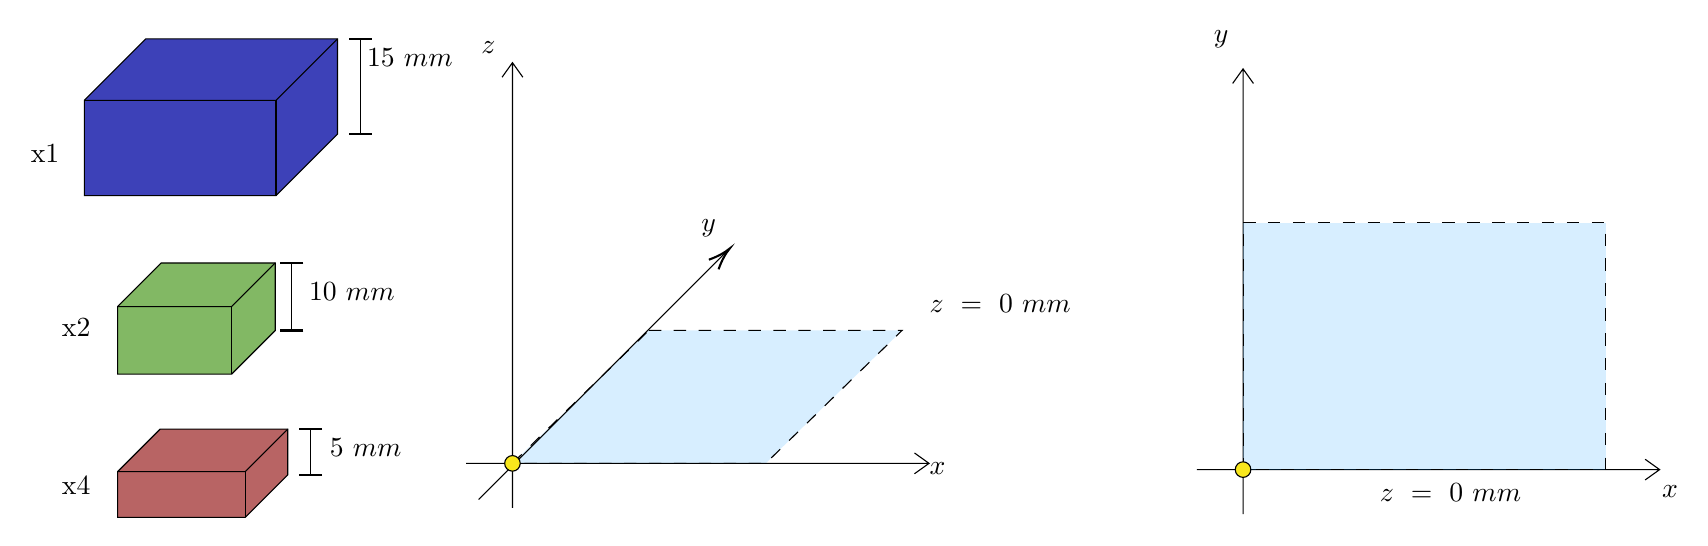
\begin{tikzpicture}[x=0.75pt,y=0.75pt,yscale=-1,xscale=1]
%uncomment if require: \path (0,285); %set diagram left start at 0, and has height of 285

%Shape: Parallelogram [id:dp9478669737271833] 
\draw  [fill={rgb, 255:red, 17; green, 154; blue, 255 }  ,fill opacity=0.17 ][dash pattern={on 4.5pt off 4.5pt}] (311,164) -- (433,164) -- (367.3,228.05) -- (245.3,228.05) -- cycle ;
%Shape: Axis 2D [id:dp9053839130374074] 
\draw  (223,228.05) -- (446,228.05)(245.3,35) -- (245.3,249.5) (439,223.05) -- (446,228.05) -- (439,233.05) (240.3,42) -- (245.3,35) -- (250.3,42)  ;
%Straight Lines [id:da1625430749081903] 
\draw    (229,245.5) -- (348.59,125.91) ;
\draw [shift={(350,124.5)}, rotate = 135] [color={rgb, 255:red, 0; green, 0; blue, 0 }  ][line width=0.75]    (10.93,-3.29) .. controls (6.95,-1.4) and (3.31,-0.3) .. (0,0) .. controls (3.31,0.3) and (6.95,1.4) .. (10.93,3.29)   ;
%Shape: Circle [id:dp5639312612319123] 
\draw  [fill={rgb, 255:red, 248; green, 231; blue, 28 }  ,fill opacity=1 ] (241.55,228.05) .. controls (241.55,225.98) and (243.23,224.3) .. (245.3,224.3) .. controls (247.37,224.3) and (249.05,225.98) .. (249.05,228.05) .. controls (249.05,230.12) and (247.37,231.8) .. (245.3,231.8) .. controls (243.23,231.8) and (241.55,230.12) .. (241.55,228.05) -- cycle ;
%Shape: Axis 2D [id:dp7452949972997148] 
\draw  (575,231.05) -- (798,231.05)(597.3,38) -- (597.3,252.5) (791,226.05) -- (798,231.05) -- (791,236.05) (592.3,45) -- (597.3,38) -- (602.3,45)  ;
%Shape: Rectangle [id:dp3032130370245537] 
\draw  [fill={rgb, 255:red, 17; green, 154; blue, 255 }  ,fill opacity=0.17 ][dash pattern={on 4.5pt off 4.5pt}] (597.3,112) -- (772,112) -- (772,231.05) -- (597.3,231.05) -- cycle ;
%Shape: Circle [id:dp4579792139014013] 
\draw  [fill={rgb, 255:red, 248; green, 231; blue, 28 }  ,fill opacity=1 ] (593.55,231.05) .. controls (593.55,228.98) and (595.23,227.3) .. (597.3,227.3) .. controls (599.37,227.3) and (601.05,228.98) .. (601.05,231.05) .. controls (601.05,233.12) and (599.37,234.8) .. (597.3,234.8) .. controls (595.23,234.8) and (593.55,233.12) .. (593.55,231.05) -- cycle ;
%Shape: Cube [id:dp562537314193528] 
\draw  [fill={rgb, 255:red, 184; green, 100; blue, 100 }  ,fill opacity=1 ] (55.05,232.05) -- (75.55,211.55) -- (137.05,211.55) -- (137.05,233.55) -- (116.55,254.05) -- (55.05,254.05) -- cycle ; \draw   (137.05,211.55) -- (116.55,232.05) -- (55.05,232.05) ; \draw   (116.55,232.05) -- (116.55,254.05) ;
%Shape: Cube [id:dp21248572948665245] 
\draw  [fill={rgb, 255:red, 130; green, 184; blue, 100 }  ,fill opacity=1 ] (55.05,152.5) -- (76.05,131.5) -- (131,131.5) -- (131,164.05) -- (110,185.05) -- (55.05,185.05) -- cycle ; \draw   (131,131.5) -- (110,152.5) -- (55.05,152.5) ; \draw   (110,152.5) -- (110,185.05) ;
%Shape: Cube [id:dp5751910582035913] 
\draw  [fill={rgb, 255:red, 61; green, 65; blue, 184 }  ,fill opacity=1 ] (39.05,53.13) -- (68.68,23.5) -- (161,23.5) -- (161,69.42) -- (131.37,99.05) -- (39.05,99.05) -- cycle ; \draw   (161,23.5) -- (131.37,53.13) -- (39.05,53.13) ; \draw   (131.37,53.13) -- (131.37,99.05) ;
%Straight Lines [id:da42543949918671464] 
\draw    (148.05,211.55) -- (148.05,233.55) ;
\draw [shift={(148.05,233.55)}, rotate = 270] [color={rgb, 255:red, 0; green, 0; blue, 0 }  ][line width=0.75]    (0,5.59) -- (0,-5.59)   ;
\draw [shift={(148.05,211.55)}, rotate = 270] [color={rgb, 255:red, 0; green, 0; blue, 0 }  ][line width=0.75]    (0,5.59) -- (0,-5.59)   ;
%Straight Lines [id:da6252654506223498] 
\draw    (139,131.5) -- (139,164.05) ;
\draw [shift={(139,164.05)}, rotate = 270] [color={rgb, 255:red, 0; green, 0; blue, 0 }  ][line width=0.75]    (0,5.59) -- (0,-5.59)   ;
\draw [shift={(139,131.5)}, rotate = 270] [color={rgb, 255:red, 0; green, 0; blue, 0 }  ][line width=0.75]    (0,5.59) -- (0,-5.59)   ;
%Straight Lines [id:da850203723421372] 
\draw    (172,23.5) -- (172,69.42) ;
\draw [shift={(172,69.42)}, rotate = 270] [color={rgb, 255:red, 0; green, 0; blue, 0 }  ][line width=0.75]    (0,5.59) -- (0,-5.59)   ;
\draw [shift={(172,23.5)}, rotate = 270] [color={rgb, 255:red, 0; green, 0; blue, 0 }  ][line width=0.75]    (0,5.59) -- (0,-5.59)   ;

% Text Node
\draw (445,145.4) node [anchor=north west][inner sep=0.75pt]    {$z\ =\ 0\ mm$};
% Text Node
\draw (335,109.4) node [anchor=north west][inner sep=0.75pt]    {$y$};
% Text Node
\draw (445,226.4) node [anchor=north west][inner sep=0.75pt]    {$x$};
% Text Node
\draw (229,23.4) node [anchor=north west][inner sep=0.75pt]    {$z$};
% Text Node
\draw (798,237.4) node [anchor=north west][inner sep=0.75pt]    {$x$};
% Text Node
\draw (582,18.4) node [anchor=north west][inner sep=0.75pt]    {$y$};
% Text Node
\draw (662,236.4) node [anchor=north west][inner sep=0.75pt]    {$z\ =\ 0\ mm$};
% Text Node
\draw (27,157) node [anchor=north west][inner sep=0.75pt]   [align=left] {x2};
% Text Node
\draw (12,73) node [anchor=north west][inner sep=0.75pt]   [align=left] {x1};
% Text Node
\draw (27,233) node [anchor=north west][inner sep=0.75pt]   [align=left] {x4};
% Text Node
\draw (156.05,214.95) node [anchor=north west][inner sep=0.75pt]    {$5\ mm$};
% Text Node
\draw (146.05,139.95) node [anchor=north west][inner sep=0.75pt]    {$10\ mm$};
% Text Node
\draw (174,26.9) node [anchor=north west][inner sep=0.75pt]    {$15\ mm$};


\end{tikzpicture}

            }
        \end{figure}
    \end{frame}
    \begin{frame}{Support Planes}
        \begin{figure}[h]
            \resizebox*{!}{65mm}{%
            

\tikzset{every picture/.style={line width=0.75pt}} %set default line width to 0.75pt        

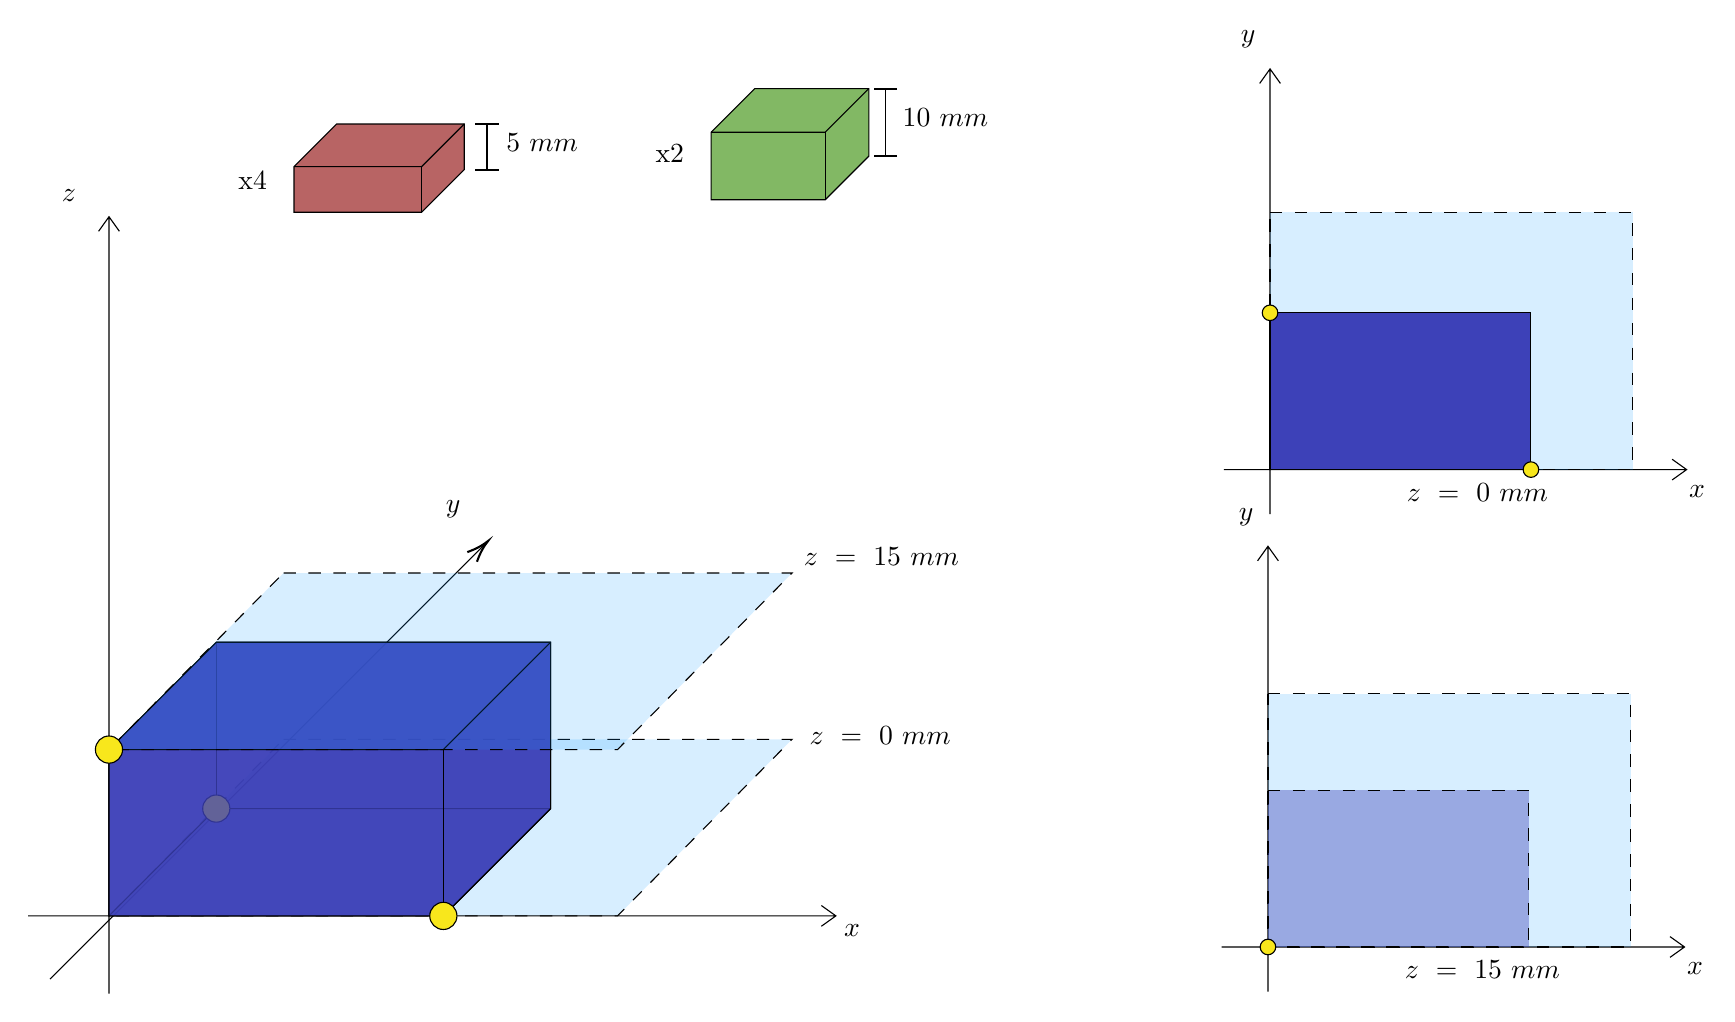
\begin{tikzpicture}[x=0.75pt,y=0.75pt,yscale=-1,xscale=1]
%uncomment if require: \path (0,526); %set diagram left start at 0, and has height of 526

%Shape: Parallelogram [id:dp4222597826124894] 
\draw  [fill={rgb, 255:red, 17; green, 154; blue, 255 }  ,fill opacity=0.17 ][dash pattern={on 4.5pt off 4.5pt}] (152,386) -- (397,386) -- (312.91,471.07) -- (67.91,471.07) -- cycle ;
%Shape: Axis 2D [id:dp7995244616027828] 
\draw  (29,471.07) -- (418.11,471.07)(67.91,134.22) -- (67.91,508.5) (411.11,466.07) -- (418.11,471.07) -- (411.11,476.07) (62.91,141.22) -- (67.91,134.22) -- (72.91,141.22)  ;
%Straight Lines [id:da046160894031782584] 
\draw    (39.47,501.52) -- (249.19,291.8) ;
\draw [shift={(250.6,290.39)}, rotate = 135] [color={rgb, 255:red, 0; green, 0; blue, 0 }  ][line width=0.75]    (10.93,-3.29) .. controls (6.95,-1.4) and (3.31,-0.3) .. (0,0) .. controls (3.31,0.3) and (6.95,1.4) .. (10.93,3.29)   ;
%Shape: Axis 2D [id:dp5764035659192752] 
\draw  (605,256.05) -- (828,256.05)(627.3,63) -- (627.3,277.5) (821,251.05) -- (828,256.05) -- (821,261.05) (622.3,70) -- (627.3,63) -- (632.3,70)  ;
%Shape: Rectangle [id:dp570599008690165] 
\draw  [fill={rgb, 255:red, 17; green, 154; blue, 255 }  ,fill opacity=0.17 ][dash pattern={on 4.5pt off 4.5pt}] (627.3,132) -- (802,132) -- (802,256.05) -- (627.3,256.05) -- cycle ;
%Shape: Cube [id:dp4526535692065705] 
\draw  [fill={rgb, 255:red, 184; green, 100; blue, 100 }  ,fill opacity=1 ] (157.05,110.05) -- (177.55,89.55) -- (239.05,89.55) -- (239.05,111.55) -- (218.55,132.05) -- (157.05,132.05) -- cycle ; \draw   (239.05,89.55) -- (218.55,110.05) -- (157.05,110.05) ; \draw   (218.55,110.05) -- (218.55,132.05) ;
%Shape: Cube [id:dp8554028533817293] 
\draw  [fill={rgb, 255:red, 130; green, 184; blue, 100 }  ,fill opacity=1 ] (358.05,93.5) -- (379.05,72.5) -- (434,72.5) -- (434,105.05) -- (413,126.05) -- (358.05,126.05) -- cycle ; \draw   (434,72.5) -- (413,93.5) -- (358.05,93.5) ; \draw   (413,93.5) -- (413,126.05) ;
%Straight Lines [id:da7979465991315938] 
\draw    (250.05,89.55) -- (250.05,111.55) ;
\draw [shift={(250.05,111.55)}, rotate = 270] [color={rgb, 255:red, 0; green, 0; blue, 0 }  ][line width=0.75]    (0,5.59) -- (0,-5.59)   ;
\draw [shift={(250.05,89.55)}, rotate = 270] [color={rgb, 255:red, 0; green, 0; blue, 0 }  ][line width=0.75]    (0,5.59) -- (0,-5.59)   ;
%Straight Lines [id:da892034196138813] 
\draw    (442,72.5) -- (442,105.05) ;
\draw [shift={(442,105.05)}, rotate = 270] [color={rgb, 255:red, 0; green, 0; blue, 0 }  ][line width=0.75]    (0,5.59) -- (0,-5.59)   ;
\draw [shift={(442,72.5)}, rotate = 270] [color={rgb, 255:red, 0; green, 0; blue, 0 }  ][line width=0.75]    (0,5.59) -- (0,-5.59)   ;
%Shape: Cube [id:dp048406160308493096] 
\draw  [fill={rgb, 255:red, 61; green, 65; blue, 184 }  ,fill opacity=0.8 ] (280.7,419.38) -- (229,471.07) -- (67.91,471.07) -- (67.91,390.94) -- (119.61,339.25) -- (280.7,339.25) -- cycle ; \draw   (67.91,471.07) -- (119.61,419.38) -- (280.7,419.38) ; \draw   (119.61,419.38) -- (119.61,339.25) ;
%Shape: Ellipse [id:dp38811273699393234] 
\draw  [fill={rgb, 255:red, 248; green, 231; blue, 28 }  ,fill opacity=1 ] (113.06,419.38) .. controls (113.06,415.76) and (115.99,412.83) .. (119.61,412.83) .. controls (123.22,412.83) and (126.15,415.76) .. (126.15,419.38) .. controls (126.15,422.99) and (123.22,425.92) .. (119.61,425.92) .. controls (115.99,425.92) and (113.06,422.99) .. (113.06,419.38) -- cycle ;
%Shape: Cube [id:dp6175116010805962] 
\draw  [fill={rgb, 255:red, 61; green, 65; blue, 184 }  ,fill opacity=0.8 ] (67.91,390.94) -- (119.61,339.25) -- (280.7,339.25) -- (280.7,419.38) -- (229,471.07) -- (67.91,471.07) -- cycle ; \draw   (280.7,339.25) -- (229,390.94) -- (67.91,390.94) ; \draw   (229,390.94) -- (229,471.07) ;
%Shape: Ellipse [id:dp8509879472929486] 
\draw  [fill={rgb, 255:red, 248; green, 231; blue, 28 }  ,fill opacity=1 ] (222.46,471.07) .. controls (222.46,467.46) and (225.39,464.53) .. (229,464.53) .. controls (232.62,464.53) and (235.55,467.46) .. (235.55,471.07) .. controls (235.55,474.69) and (232.62,477.62) .. (229,477.62) .. controls (225.39,477.62) and (222.46,474.69) .. (222.46,471.07) -- cycle ;
%Shape: Axis 2D [id:dp48062019416570856] 
\draw  (604,486.05) -- (827,486.05)(626.3,293) -- (626.3,507.5) (820,481.05) -- (827,486.05) -- (820,491.05) (621.3,300) -- (626.3,293) -- (631.3,300)  ;
%Shape: Rectangle [id:dp2573254178626563] 
\draw  [fill={rgb, 255:red, 17; green, 154; blue, 255 }  ,fill opacity=0.17 ][dash pattern={on 4.5pt off 4.5pt}] (626.3,364) -- (801,364) -- (801,486.05) -- (626.3,486.05) -- cycle ;
%Shape: Rectangle [id:dp8530743639576063] 
\draw  [fill={rgb, 255:red, 61; green, 65; blue, 184 }  ,fill opacity=1 ] (627.3,180.5) -- (753,180.5) -- (753,256.05) -- (627.3,256.05) -- cycle ;
%Shape: Circle [id:dp9590370044899046] 
\draw  [fill={rgb, 255:red, 248; green, 231; blue, 28 }  ,fill opacity=1 ] (623.55,180.5) .. controls (623.55,178.43) and (625.23,176.75) .. (627.3,176.75) .. controls (629.37,176.75) and (631.05,178.43) .. (631.05,180.5) .. controls (631.05,182.57) and (629.37,184.25) .. (627.3,184.25) .. controls (625.23,184.25) and (623.55,182.57) .. (623.55,180.5) -- cycle ;
%Shape: Circle [id:dp7919472039444115] 
\draw  [fill={rgb, 255:red, 248; green, 231; blue, 28 }  ,fill opacity=1 ] (749.25,256.05) .. controls (749.25,253.98) and (750.93,252.3) .. (753,252.3) .. controls (755.07,252.3) and (756.75,253.98) .. (756.75,256.05) .. controls (756.75,258.12) and (755.07,259.8) .. (753,259.8) .. controls (750.93,259.8) and (749.25,258.12) .. (749.25,256.05) -- cycle ;
%Shape: Rectangle [id:dp2993308124270544] 
\draw  [fill={rgb, 255:red, 61; green, 65; blue, 184 }  ,fill opacity=0.4 ][dash pattern={on 4.5pt off 4.5pt}] (626.3,410.5) -- (752,410.5) -- (752,486.05) -- (626.3,486.05) -- cycle ;
%Shape: Circle [id:dp16199792658724443] 
\draw  [fill={rgb, 255:red, 248; green, 231; blue, 28 }  ,fill opacity=1 ] (622.55,486.05) .. controls (622.55,483.98) and (624.23,482.3) .. (626.3,482.3) .. controls (628.37,482.3) and (630.05,483.98) .. (630.05,486.05) .. controls (630.05,488.12) and (628.37,489.8) .. (626.3,489.8) .. controls (624.23,489.8) and (622.55,488.12) .. (622.55,486.05) -- cycle ;
%Shape: Parallelogram [id:dp1306220090712341] 
\draw  [fill={rgb, 255:red, 17; green, 154; blue, 255 }  ,fill opacity=0.17 ][dash pattern={on 4.5pt off 4.5pt}] (152,305.87) -- (397,305.87) -- (312.91,390.94) -- (67.91,390.94) -- cycle ;
%Shape: Ellipse [id:dp7884999653092057] 
\draw  [fill={rgb, 255:red, 248; green, 231; blue, 28 }  ,fill opacity=1 ] (61.37,390.94) .. controls (61.37,387.33) and (64.3,384.4) .. (67.91,384.4) .. controls (71.52,384.4) and (74.45,387.33) .. (74.45,390.94) .. controls (74.45,394.56) and (71.52,397.49) .. (67.91,397.49) .. controls (64.3,397.49) and (61.37,394.56) .. (61.37,390.94) -- cycle ;

% Text Node
\draw (228.9,269.7) node [anchor=north west][inner sep=0.75pt]    {$y$};
% Text Node
\draw (420.84,473.85) node [anchor=north west][inner sep=0.75pt]    {$x$};
% Text Node
\draw (43.94,119.64) node [anchor=north west][inner sep=0.75pt]    {$z$};
% Text Node
\draw (828,262.4) node [anchor=north west][inner sep=0.75pt]    {$x$};
% Text Node
\draw (612,43.4) node [anchor=north west][inner sep=0.75pt]    {$y$};
% Text Node
\draw (692,261.4) node [anchor=north west][inner sep=0.75pt]    {$z\ =\ 0\ mm$};
% Text Node
\draw (330,98) node [anchor=north west][inner sep=0.75pt]   [align=left] {x2};
% Text Node
\draw (129,111) node [anchor=north west][inner sep=0.75pt]   [align=left] {x4};
% Text Node
\draw (258.05,92.95) node [anchor=north west][inner sep=0.75pt]    {$5\ mm$};
% Text Node
\draw (449.05,80.95) node [anchor=north west][inner sep=0.75pt]    {$10\ mm$};
% Text Node
\draw (827,492.4) node [anchor=north west][inner sep=0.75pt]    {$x$};
% Text Node
\draw (611,273.4) node [anchor=north west][inner sep=0.75pt]    {$y$};
% Text Node
\draw (691,491.4) node [anchor=north west][inner sep=0.75pt]    {$z\ =\ 15\ mm$};
% Text Node
\draw (404.19,378.66) node [anchor=north west][inner sep=0.75pt]    {$z\ =\ 0\ mm$};
% Text Node
\draw (401.48,292.2) node [anchor=north west][inner sep=0.75pt]    {$z\ =\ 15\ mm$};


\end{tikzpicture}

            }
        \end{figure}
    \end{frame}
    \begin{frame}{Support Planes}
        \begin{figure}[h]
            \resizebox*{!}{65mm}{%
            

\tikzset{every picture/.style={line width=0.75pt}} %set default line width to 0.75pt        

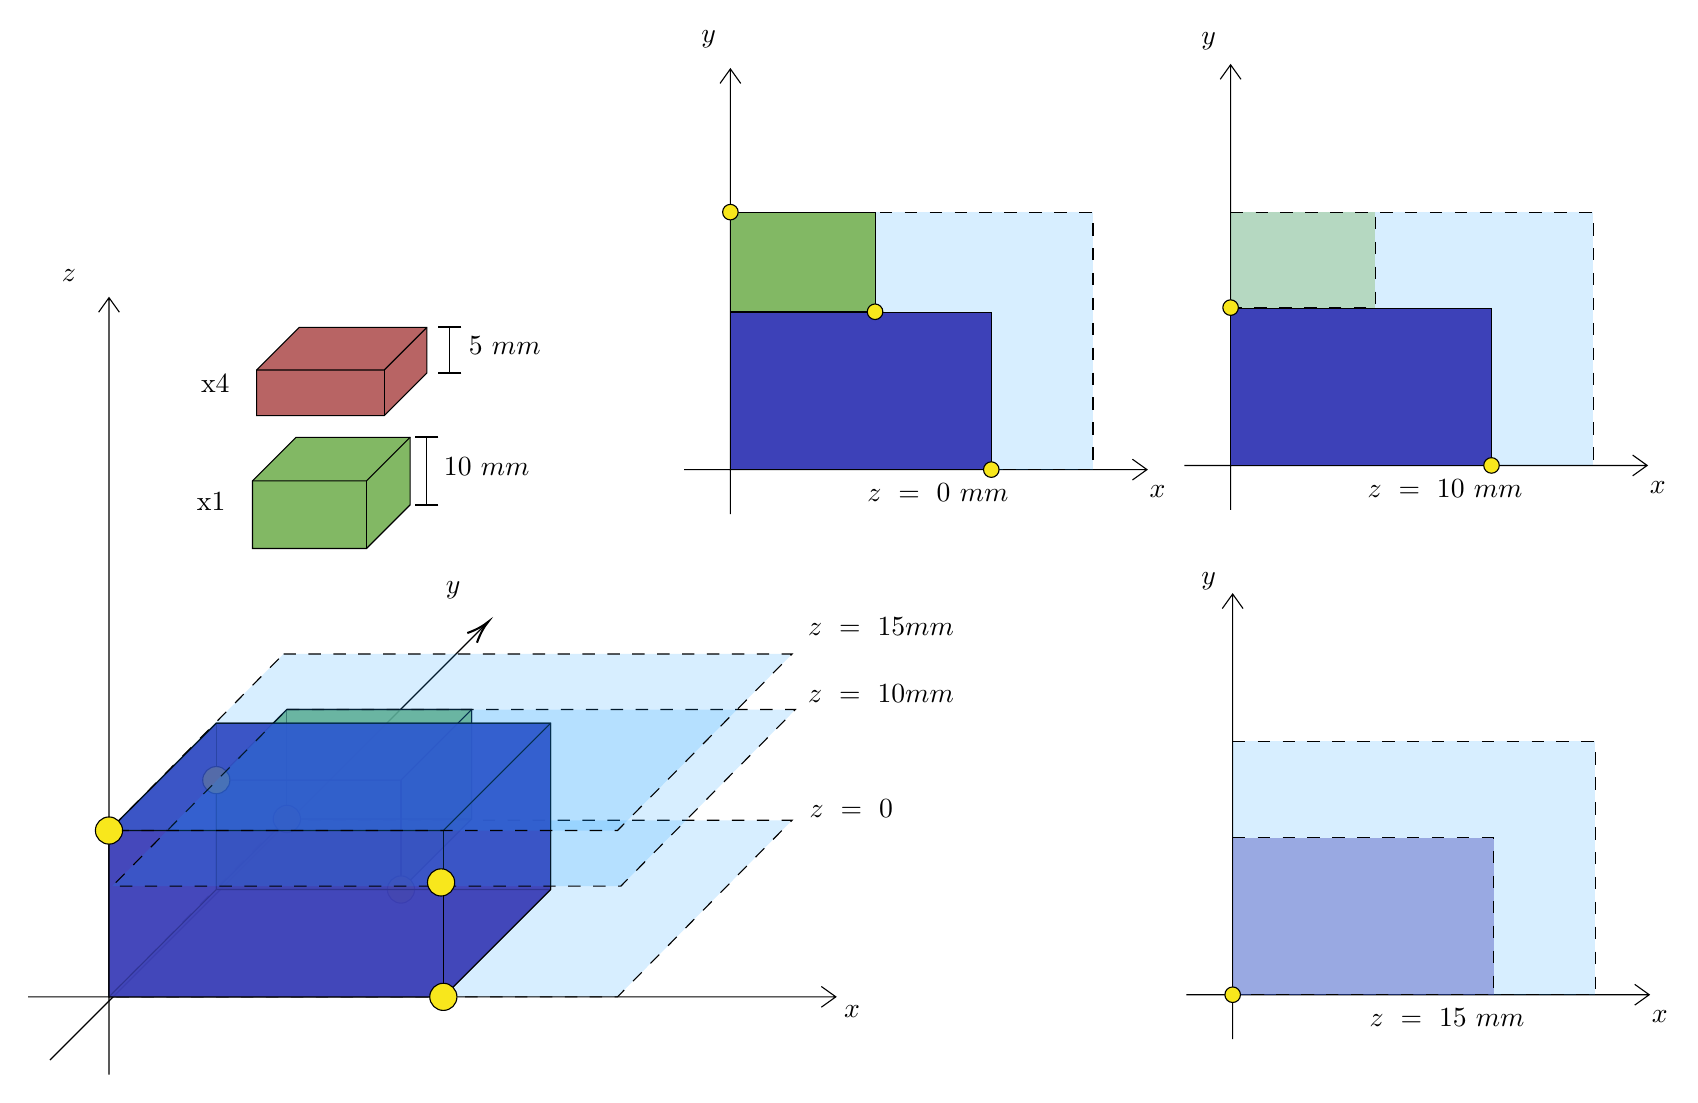
\begin{tikzpicture}[x=0.75pt,y=0.75pt,yscale=-1,xscale=1]
%uncomment if require: \path (0,538); %set diagram left start at 0, and has height of 538

%Shape: Parallelogram [id:dp09178640407068794] 
\draw  [fill={rgb, 255:red, 17; green, 154; blue, 255 }  ,fill opacity=0.17 ][dash pattern={on 4.5pt off 4.5pt}] (140,398) -- (385,398) -- (300.91,483.07) -- (55.91,483.07) -- cycle ;
%Shape: Axis 2D [id:dp8258852857376601] 
\draw  (17,483.07) -- (406.11,483.07)(55.91,146.22) -- (55.91,520.5) (399.11,478.07) -- (406.11,483.07) -- (399.11,488.07) (50.91,153.22) -- (55.91,146.22) -- (60.91,153.22)  ;
%Straight Lines [id:da550852979816048] 
\draw    (27.47,513.52) -- (237.19,303.8) ;
\draw [shift={(238.6,302.39)}, rotate = 135] [color={rgb, 255:red, 0; green, 0; blue, 0 }  ][line width=0.75]    (10.93,-3.29) .. controls (6.95,-1.4) and (3.31,-0.3) .. (0,0) .. controls (3.31,0.3) and (6.95,1.4) .. (10.93,3.29)   ;
%Shape: Cube [id:dp14680549395170983] 
\draw  [fill={rgb, 255:red, 184; green, 100; blue, 100 }  ,fill opacity=1 ] (127.05,181.05) -- (147.55,160.55) -- (209.05,160.55) -- (209.05,182.55) -- (188.55,203.05) -- (127.05,203.05) -- cycle ; \draw   (209.05,160.55) -- (188.55,181.05) -- (127.05,181.05) ; \draw   (188.55,181.05) -- (188.55,203.05) ;
%Shape: Cube [id:dp46712490024212483] 
\draw  [fill={rgb, 255:red, 130; green, 184; blue, 100 }  ,fill opacity=1 ] (125.05,234.5) -- (146.05,213.5) -- (201,213.5) -- (201,246.05) -- (180,267.05) -- (125.05,267.05) -- cycle ; \draw   (201,213.5) -- (180,234.5) -- (125.05,234.5) ; \draw   (180,234.5) -- (180,267.05) ;
%Straight Lines [id:da6118159593170233] 
\draw    (220.05,160.55) -- (220.05,182.55) ;
\draw [shift={(220.05,182.55)}, rotate = 270] [color={rgb, 255:red, 0; green, 0; blue, 0 }  ][line width=0.75]    (0,5.59) -- (0,-5.59)   ;
\draw [shift={(220.05,160.55)}, rotate = 270] [color={rgb, 255:red, 0; green, 0; blue, 0 }  ][line width=0.75]    (0,5.59) -- (0,-5.59)   ;
%Straight Lines [id:da5742168927770045] 
\draw    (209,213.5) -- (209,246.05) ;
\draw [shift={(209,246.05)}, rotate = 270] [color={rgb, 255:red, 0; green, 0; blue, 0 }  ][line width=0.75]    (0,5.59) -- (0,-5.59)   ;
\draw [shift={(209,213.5)}, rotate = 270] [color={rgb, 255:red, 0; green, 0; blue, 0 }  ][line width=0.75]    (0,5.59) -- (0,-5.59)   ;
%Shape: Cube [id:dp02477282881593157] 
\draw  [fill={rgb, 255:red, 130; green, 184; blue, 100 }  ,fill opacity=0.63 ] (230.6,397.37) -- (196.6,431.38) -- (107.61,431.38) -- (107.61,378.66) -- (141.62,344.65) -- (230.6,344.65) -- cycle ; \draw   (107.61,431.38) -- (141.62,397.37) -- (230.6,397.37) ; \draw   (141.62,397.37) -- (141.62,344.65) ;
%Shape: Cube [id:dp20821489285755002] 
\draw  [fill={rgb, 255:red, 130; green, 184; blue, 100 }  ,fill opacity=0.63 ] (107.61,378.66) -- (141.62,344.65) -- (230.6,344.65) -- (230.6,397.37) -- (196.6,431.38) -- (107.61,431.38) -- cycle ; \draw   (230.6,344.65) -- (196.6,378.66) -- (107.61,378.66) ; \draw   (196.6,378.66) -- (196.6,431.38) ;
%Shape: Ellipse [id:dp2106830815169426] 
\draw  [fill={rgb, 255:red, 248; green, 231; blue, 28 }  ,fill opacity=1 ] (135.07,397.37) .. controls (135.07,393.75) and (138,390.82) .. (141.62,390.82) .. controls (145.23,390.82) and (148.16,393.75) .. (148.16,397.37) .. controls (148.16,400.98) and (145.23,403.91) .. (141.62,403.91) .. controls (138,403.91) and (135.07,400.98) .. (135.07,397.37) -- cycle ;
%Shape: Ellipse [id:dp9136393646434955] 
\draw  [fill={rgb, 255:red, 248; green, 231; blue, 28 }  ,fill opacity=1 ] (190.05,431.38) .. controls (190.05,427.76) and (192.98,424.83) .. (196.6,424.83) .. controls (200.21,424.83) and (203.14,427.76) .. (203.14,431.38) .. controls (203.14,434.99) and (200.21,437.92) .. (196.6,437.92) .. controls (192.98,437.92) and (190.05,434.99) .. (190.05,431.38) -- cycle ;
%Shape: Axis 2D [id:dp847355347947621] 
\draw  (333,229.05) -- (556,229.05)(355.3,36) -- (355.3,250.5) (549,224.05) -- (556,229.05) -- (549,234.05) (350.3,43) -- (355.3,36) -- (360.3,43)  ;
%Shape: Rectangle [id:dp7766208548232109] 
\draw  [fill={rgb, 255:red, 17; green, 154; blue, 255 }  ,fill opacity=0.17 ][dash pattern={on 4.5pt off 4.5pt}] (355.3,105) -- (530,105) -- (530,229.05) -- (355.3,229.05) -- cycle ;
%Shape: Axis 2D [id:dp7714903402225337] 
\draw  (575,482.05) -- (798,482.05)(597.3,289) -- (597.3,503.5) (791,477.05) -- (798,482.05) -- (791,487.05) (592.3,296) -- (597.3,289) -- (602.3,296)  ;
%Shape: Rectangle [id:dp9401991311225601] 
\draw  [fill={rgb, 255:red, 17; green, 154; blue, 255 }  ,fill opacity=0.17 ][dash pattern={on 4.5pt off 4.5pt}] (597.3,360) -- (772,360) -- (772,482.05) -- (597.3,482.05) -- cycle ;
%Shape: Rectangle [id:dp9613638080642445] 
\draw  [fill={rgb, 255:red, 61; green, 65; blue, 184 }  ,fill opacity=1 ] (355.3,153.5) -- (481,153.5) -- (481,229.05) -- (355.3,229.05) -- cycle ;
%Shape: Circle [id:dp9007780724895271] 
\draw  [fill={rgb, 255:red, 248; green, 231; blue, 28 }  ,fill opacity=1 ] (477.25,229.05) .. controls (477.25,226.98) and (478.93,225.3) .. (481,225.3) .. controls (483.07,225.3) and (484.75,226.98) .. (484.75,229.05) .. controls (484.75,231.12) and (483.07,232.8) .. (481,232.8) .. controls (478.93,232.8) and (477.25,231.12) .. (477.25,229.05) -- cycle ;
%Shape: Rectangle [id:dp9460893732722917] 
\draw  [fill={rgb, 255:red, 61; green, 65; blue, 184 }  ,fill opacity=0.4 ][dash pattern={on 4.5pt off 4.5pt}] (597.3,406.5) -- (723,406.5) -- (723,482.05) -- (597.3,482.05) -- cycle ;
%Shape: Circle [id:dp9223398880117945] 
\draw  [fill={rgb, 255:red, 248; green, 231; blue, 28 }  ,fill opacity=1 ] (593.55,482.05) .. controls (593.55,479.98) and (595.23,478.3) .. (597.3,478.3) .. controls (599.37,478.3) and (601.05,479.98) .. (601.05,482.05) .. controls (601.05,484.12) and (599.37,485.8) .. (597.3,485.8) .. controls (595.23,485.8) and (593.55,484.12) .. (593.55,482.05) -- cycle ;
%Shape: Cube [id:dp7165924837156505] 
\draw  [fill={rgb, 255:red, 61; green, 65; blue, 184 }  ,fill opacity=0.8 ] (268.7,431.38) -- (217,483.07) -- (55.91,483.07) -- (55.91,402.94) -- (107.61,351.25) -- (268.7,351.25) -- cycle ; \draw   (55.91,483.07) -- (107.61,431.38) -- (268.7,431.38) ; \draw   (107.61,431.38) -- (107.61,351.25) ;
%Shape: Ellipse [id:dp6646122819236989] 
\draw  [fill={rgb, 255:red, 248; green, 231; blue, 28 }  ,fill opacity=1 ] (101.06,378.66) .. controls (101.06,375.05) and (103.99,372.12) .. (107.61,372.12) .. controls (111.22,372.12) and (114.15,375.05) .. (114.15,378.66) .. controls (114.15,382.28) and (111.22,385.21) .. (107.61,385.21) .. controls (103.99,385.21) and (101.06,382.28) .. (101.06,378.66) -- cycle ;
%Shape: Cube [id:dp47660454367889615] 
\draw  [fill={rgb, 255:red, 61; green, 65; blue, 184 }  ,fill opacity=0.8 ] (55.91,402.94) -- (107.61,351.25) -- (268.7,351.25) -- (268.7,431.38) -- (217,483.07) -- (55.91,483.07) -- cycle ; \draw   (268.7,351.25) -- (217,402.94) -- (55.91,402.94) ; \draw   (217,402.94) -- (217,483.07) ;
%Shape: Ellipse [id:dp5192134071707744] 
\draw  [fill={rgb, 255:red, 248; green, 231; blue, 28 }  ,fill opacity=1 ] (210.46,483.07) .. controls (210.46,479.46) and (213.39,476.53) .. (217,476.53) .. controls (220.62,476.53) and (223.55,479.46) .. (223.55,483.07) .. controls (223.55,486.69) and (220.62,489.62) .. (217,489.62) .. controls (213.39,489.62) and (210.46,486.69) .. (210.46,483.07) -- cycle ;
%Shape: Rectangle [id:dp7840813076850105] 
\draw  [fill={rgb, 255:red, 130; green, 184; blue, 100 }  ,fill opacity=1 ] (355.3,105) -- (425,105) -- (425,153) -- (355.3,153) -- cycle ;
%Shape: Axis 2D [id:dp13043741429807865] 
\draw  (574,227.05) -- (797,227.05)(596.3,34) -- (596.3,248.5) (790,222.05) -- (797,227.05) -- (790,232.05) (591.3,41) -- (596.3,34) -- (601.3,41)  ;
%Shape: Rectangle [id:dp7230411548725182] 
\draw  [fill={rgb, 255:red, 17; green, 154; blue, 255 }  ,fill opacity=0.17 ][dash pattern={on 4.5pt off 4.5pt}] (596.3,105) -- (771,105) -- (771,227.05) -- (596.3,227.05) -- cycle ;
%Shape: Rectangle [id:dp22750009363961254] 
\draw  [fill={rgb, 255:red, 61; green, 65; blue, 184 }  ,fill opacity=1 ] (596.3,151.5) -- (722,151.5) -- (722,227.05) -- (596.3,227.05) -- cycle ;
%Shape: Rectangle [id:dp7681823656621036] 
\draw  [fill={rgb, 255:red, 130; green, 184; blue, 100 }  ,fill opacity=0.4 ][dash pattern={on 4.5pt off 4.5pt}] (596.3,105) -- (666,105) -- (666,151) -- (596.3,151) -- cycle ;
%Shape: Circle [id:dp9437675985021478] 
\draw  [fill={rgb, 255:red, 248; green, 231; blue, 28 }  ,fill opacity=1 ] (592.55,151) .. controls (592.55,148.93) and (594.23,147.25) .. (596.3,147.25) .. controls (598.37,147.25) and (600.05,148.93) .. (600.05,151) .. controls (600.05,153.07) and (598.37,154.75) .. (596.3,154.75) .. controls (594.23,154.75) and (592.55,153.07) .. (592.55,151) -- cycle ;
%Shape: Circle [id:dp5193325720283657] 
\draw  [fill={rgb, 255:red, 248; green, 231; blue, 28 }  ,fill opacity=1 ] (718.25,227.05) .. controls (718.25,224.98) and (719.93,223.3) .. (722,223.3) .. controls (724.07,223.3) and (725.75,224.98) .. (725.75,227.05) .. controls (725.75,229.12) and (724.07,230.8) .. (722,230.8) .. controls (719.93,230.8) and (718.25,229.12) .. (718.25,227.05) -- cycle ;
%Shape: Circle [id:dp5534395845488237] 
\draw  [fill={rgb, 255:red, 248; green, 231; blue, 28 }  ,fill opacity=1 ] (421.25,153) .. controls (421.25,150.93) and (422.93,149.25) .. (425,149.25) .. controls (427.07,149.25) and (428.75,150.93) .. (428.75,153) .. controls (428.75,155.07) and (427.07,156.75) .. (425,156.75) .. controls (422.93,156.75) and (421.25,155.07) .. (421.25,153) -- cycle ;
%Shape: Circle [id:dp7899938903984195] 
\draw  [fill={rgb, 255:red, 248; green, 231; blue, 28 }  ,fill opacity=1 ] (351.55,105) .. controls (351.55,102.93) and (353.23,101.25) .. (355.3,101.25) .. controls (357.37,101.25) and (359.05,102.93) .. (359.05,105) .. controls (359.05,107.07) and (357.37,108.75) .. (355.3,108.75) .. controls (353.23,108.75) and (351.55,107.07) .. (351.55,105) -- cycle ;
%Shape: Parallelogram [id:dp11964271185731867] 
\draw  [fill={rgb, 255:red, 17; green, 154; blue, 255 }  ,fill opacity=0.17 ][dash pattern={on 4.5pt off 4.5pt}] (141.62,344.65) -- (386.62,344.65) -- (302.53,429.73) -- (57.53,429.73) -- cycle ;
%Shape: Ellipse [id:dp9177289108057064] 
\draw  [fill={rgb, 255:red, 248; green, 231; blue, 28 }  ,fill opacity=1 ] (209.37,427.94) .. controls (209.37,424.33) and (212.3,421.4) .. (215.91,421.4) .. controls (219.52,421.4) and (222.45,424.33) .. (222.45,427.94) .. controls (222.45,431.56) and (219.52,434.49) .. (215.91,434.49) .. controls (212.3,434.49) and (209.37,431.56) .. (209.37,427.94) -- cycle ;
%Shape: Parallelogram [id:dp2459754259636302] 
\draw  [fill={rgb, 255:red, 17; green, 154; blue, 255 }  ,fill opacity=0.17 ][dash pattern={on 4.5pt off 4.5pt}] (140,317.87) -- (385,317.87) -- (300.91,402.94) -- (55.91,402.94) -- cycle ;
%Shape: Ellipse [id:dp5262514948515243] 
\draw  [fill={rgb, 255:red, 248; green, 231; blue, 28 }  ,fill opacity=1 ] (49.37,402.94) .. controls (49.37,399.33) and (52.3,396.4) .. (55.91,396.4) .. controls (59.52,396.4) and (62.45,399.33) .. (62.45,402.94) .. controls (62.45,406.56) and (59.52,409.49) .. (55.91,409.49) .. controls (52.3,409.49) and (49.37,406.56) .. (49.37,402.94) -- cycle ;

% Text Node
\draw (392.19,386.66) node [anchor=north west][inner sep=0.75pt]    {$z\ =\ 0$};
% Text Node
\draw (216.9,281.7) node [anchor=north west][inner sep=0.75pt]    {$y$};
% Text Node
\draw (408.84,485.85) node [anchor=north west][inner sep=0.75pt]    {$x$};
% Text Node
\draw (31.94,131.64) node [anchor=north west][inner sep=0.75pt]    {$z$};
% Text Node
\draw (97,239) node [anchor=north west][inner sep=0.75pt]   [align=left] {x1};
% Text Node
\draw (99,182) node [anchor=north west][inner sep=0.75pt]   [align=left] {x4};
% Text Node
\draw (228.05,163.95) node [anchor=north west][inner sep=0.75pt]    {$5\ mm$};
% Text Node
\draw (216.05,221.95) node [anchor=north west][inner sep=0.75pt]    {$10\ mm$};
% Text Node
\draw (391.48,299.2) node [anchor=north west][inner sep=0.75pt]    {$z\ =\ 15mm$};
% Text Node
\draw (556,235.4) node [anchor=north west][inner sep=0.75pt]    {$x$};
% Text Node
\draw (340,16.4) node [anchor=north west][inner sep=0.75pt]    {$y$};
% Text Node
\draw (420,234.4) node [anchor=north west][inner sep=0.75pt]    {$z\ =\ 0\ mm$};
% Text Node
\draw (798,488.4) node [anchor=north west][inner sep=0.75pt]    {$x$};
% Text Node
\draw (581,17.4) node [anchor=north west][inner sep=0.75pt]    {$y$};
% Text Node
\draw (662,487.4) node [anchor=north west][inner sep=0.75pt]    {$z\ =\ 15\ mm$};
% Text Node
\draw (391.48,331.2) node [anchor=north west][inner sep=0.75pt]    {$z\ =\ 10mm$};
% Text Node
\draw (797,233.4) node [anchor=north west][inner sep=0.75pt]    {$x$};
% Text Node
\draw (661,232.4) node [anchor=north west][inner sep=0.75pt]    {$z\ =\ 10\ mm$};
% Text Node
\draw (581,277.4) node [anchor=north west][inner sep=0.75pt]    {$y$};


\end{tikzpicture}

            }
        \end{figure}
    \end{frame}
    \begin{frame}{Support Planes}
        \begin{figure}[h]
            \resizebox*{!}{65mm}{%
            

\tikzset{every picture/.style={line width=0.75pt}} %set default line width to 0.75pt        

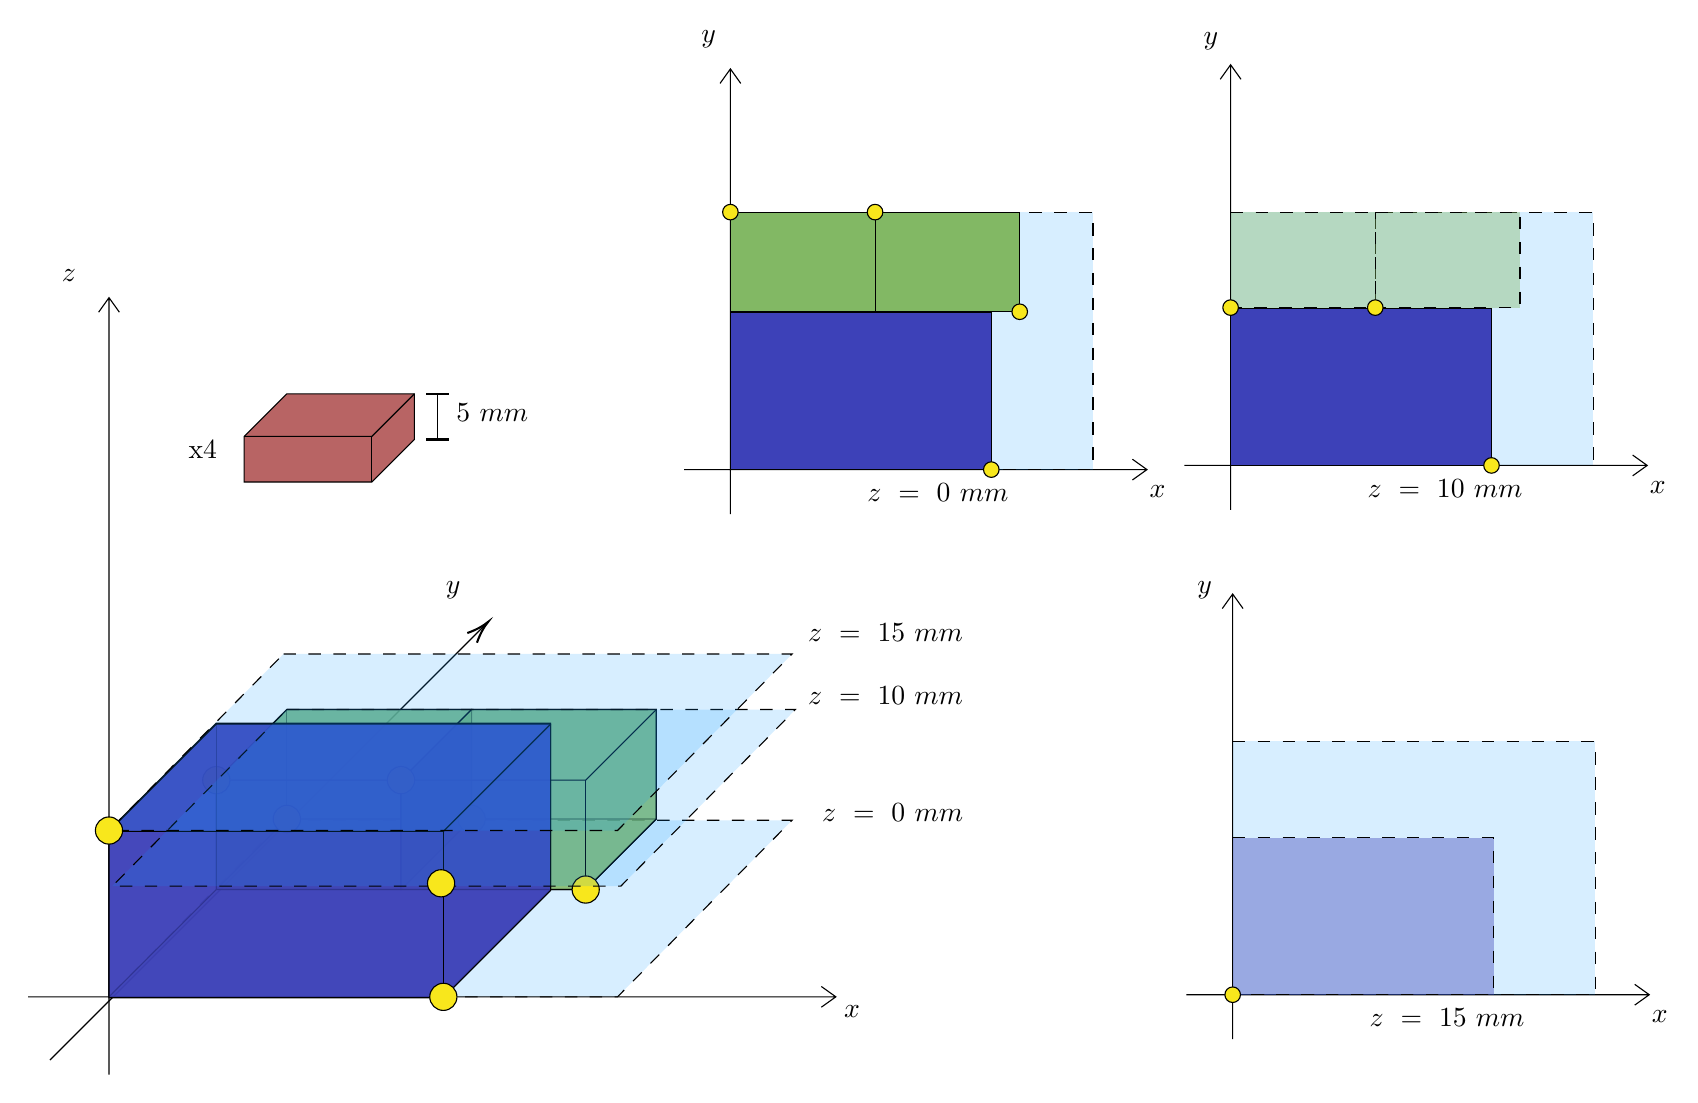
\begin{tikzpicture}[x=0.75pt,y=0.75pt,yscale=-1,xscale=1]
%uncomment if require: \path (0,534); %set diagram left start at 0, and has height of 534

%Shape: Parallelogram [id:dp7751366201442232] 
\draw  [fill={rgb, 255:red, 17; green, 154; blue, 255 }  ,fill opacity=0.17 ][dash pattern={on 4.5pt off 4.5pt}] (160,401.5) -- (405,401.5) -- (320.91,486.57) -- (75.91,486.57) -- cycle ;
%Shape: Axis 2D [id:dp3837723600064221] 
\draw  (37,486.57) -- (426.11,486.57)(75.91,149.72) -- (75.91,524) (419.11,481.57) -- (426.11,486.57) -- (419.11,491.57) (70.91,156.72) -- (75.91,149.72) -- (80.91,156.72)  ;
%Straight Lines [id:da8847163778900521] 
\draw    (47.47,517.02) -- (257.19,307.3) ;
\draw [shift={(258.6,305.89)}, rotate = 135] [color={rgb, 255:red, 0; green, 0; blue, 0 }  ][line width=0.75]    (10.93,-3.29) .. controls (6.95,-1.4) and (3.31,-0.3) .. (0,0) .. controls (3.31,0.3) and (6.95,1.4) .. (10.93,3.29)   ;
%Shape: Cube [id:dp3635830050945964] 
\draw  [fill={rgb, 255:red, 184; green, 100; blue, 100 }  ,fill opacity=1 ] (141.05,216.55) -- (161.55,196.05) -- (223.05,196.05) -- (223.05,218.05) -- (202.55,238.55) -- (141.05,238.55) -- cycle ; \draw   (223.05,196.05) -- (202.55,216.55) -- (141.05,216.55) ; \draw   (202.55,216.55) -- (202.55,238.55) ;
%Straight Lines [id:da20863712965836156] 
\draw    (234.05,196.05) -- (234.05,218.05) ;
\draw [shift={(234.05,218.05)}, rotate = 270] [color={rgb, 255:red, 0; green, 0; blue, 0 }  ][line width=0.75]    (0,5.59) -- (0,-5.59)   ;
\draw [shift={(234.05,196.05)}, rotate = 270] [color={rgb, 255:red, 0; green, 0; blue, 0 }  ][line width=0.75]    (0,5.59) -- (0,-5.59)   ;
%Shape: Cube [id:dp14901885435262208] 
\draw  [fill={rgb, 255:red, 130; green, 184; blue, 100 }  ,fill opacity=0.63 ] (250.6,400.87) -- (216.6,434.88) -- (127.61,434.88) -- (127.61,382.16) -- (161.62,348.15) -- (250.6,348.15) -- cycle ; \draw   (127.61,434.88) -- (161.62,400.87) -- (250.6,400.87) ; \draw   (161.62,400.87) -- (161.62,348.15) ;
%Shape: Cube [id:dp04953927607727482] 
\draw  [fill={rgb, 255:red, 130; green, 184; blue, 100 }  ,fill opacity=0.63 ] (127.61,382.16) -- (161.62,348.15) -- (250.6,348.15) -- (250.6,400.87) -- (216.6,434.88) -- (127.61,434.88) -- cycle ; \draw   (250.6,348.15) -- (216.6,382.16) -- (127.61,382.16) ; \draw   (216.6,382.16) -- (216.6,434.88) ;
%Shape: Ellipse [id:dp16065081118970448] 
\draw  [fill={rgb, 255:red, 248; green, 231; blue, 28 }  ,fill opacity=1 ] (155.07,400.87) .. controls (155.07,397.25) and (158,394.32) .. (161.62,394.32) .. controls (165.23,394.32) and (168.16,397.25) .. (168.16,400.87) .. controls (168.16,404.48) and (165.23,407.41) .. (161.62,407.41) .. controls (158,407.41) and (155.07,404.48) .. (155.07,400.87) -- cycle ;
%Shape: Axis 2D [id:dp19619353602022283] 
\draw  (353,232.55) -- (576,232.55)(375.3,39.5) -- (375.3,254) (569,227.55) -- (576,232.55) -- (569,237.55) (370.3,46.5) -- (375.3,39.5) -- (380.3,46.5)  ;
%Shape: Rectangle [id:dp33143452408930063] 
\draw  [fill={rgb, 255:red, 17; green, 154; blue, 255 }  ,fill opacity=0.17 ][dash pattern={on 4.5pt off 4.5pt}] (375.3,108.5) -- (550,108.5) -- (550,232.55) -- (375.3,232.55) -- cycle ;
%Shape: Axis 2D [id:dp5481878343423418] 
\draw  (595,485.55) -- (818,485.55)(617.3,292.5) -- (617.3,507) (811,480.55) -- (818,485.55) -- (811,490.55) (612.3,299.5) -- (617.3,292.5) -- (622.3,299.5)  ;
%Shape: Rectangle [id:dp0751382303539937] 
\draw  [fill={rgb, 255:red, 17; green, 154; blue, 255 }  ,fill opacity=0.17 ][dash pattern={on 4.5pt off 4.5pt}] (617.3,363.5) -- (792,363.5) -- (792,485.55) -- (617.3,485.55) -- cycle ;
%Shape: Rectangle [id:dp6629808163615512] 
\draw  [fill={rgb, 255:red, 61; green, 65; blue, 184 }  ,fill opacity=1 ] (375.3,157) -- (501,157) -- (501,232.55) -- (375.3,232.55) -- cycle ;
%Shape: Circle [id:dp35911666707702883] 
\draw  [fill={rgb, 255:red, 248; green, 231; blue, 28 }  ,fill opacity=1 ] (497.25,232.55) .. controls (497.25,230.48) and (498.93,228.8) .. (501,228.8) .. controls (503.07,228.8) and (504.75,230.48) .. (504.75,232.55) .. controls (504.75,234.62) and (503.07,236.3) .. (501,236.3) .. controls (498.93,236.3) and (497.25,234.62) .. (497.25,232.55) -- cycle ;
%Shape: Rectangle [id:dp013264087552227966] 
\draw  [fill={rgb, 255:red, 61; green, 65; blue, 184 }  ,fill opacity=0.4 ][dash pattern={on 4.5pt off 4.5pt}] (617.3,410) -- (743,410) -- (743,485.55) -- (617.3,485.55) -- cycle ;
%Shape: Circle [id:dp6077371981928216] 
\draw  [fill={rgb, 255:red, 248; green, 231; blue, 28 }  ,fill opacity=1 ] (613.55,485.55) .. controls (613.55,483.48) and (615.23,481.8) .. (617.3,481.8) .. controls (619.37,481.8) and (621.05,483.48) .. (621.05,485.55) .. controls (621.05,487.62) and (619.37,489.3) .. (617.3,489.3) .. controls (615.23,489.3) and (613.55,487.62) .. (613.55,485.55) -- cycle ;
%Shape: Ellipse [id:dp8407817298450738] 
\draw  [fill={rgb, 255:red, 248; green, 231; blue, 28 }  ,fill opacity=1 ] (121.06,382.16) .. controls (121.06,378.55) and (123.99,375.62) .. (127.61,375.62) .. controls (131.22,375.62) and (134.15,378.55) .. (134.15,382.16) .. controls (134.15,385.78) and (131.22,388.71) .. (127.61,388.71) .. controls (123.99,388.71) and (121.06,385.78) .. (121.06,382.16) -- cycle ;
%Shape: Rectangle [id:dp4579626963483141] 
\draw  [fill={rgb, 255:red, 130; green, 184; blue, 100 }  ,fill opacity=1 ] (375.3,108.5) -- (445,108.5) -- (445,156.5) -- (375.3,156.5) -- cycle ;
%Shape: Axis 2D [id:dp030146975396011744] 
\draw  (594,230.55) -- (817,230.55)(616.3,37.5) -- (616.3,252) (810,225.55) -- (817,230.55) -- (810,235.55) (611.3,44.5) -- (616.3,37.5) -- (621.3,44.5)  ;
%Shape: Rectangle [id:dp1502605037988708] 
\draw  [fill={rgb, 255:red, 17; green, 154; blue, 255 }  ,fill opacity=0.17 ][dash pattern={on 4.5pt off 4.5pt}] (616.3,108.5) -- (791,108.5) -- (791,230.55) -- (616.3,230.55) -- cycle ;
%Shape: Rectangle [id:dp7799690060157576] 
\draw  [fill={rgb, 255:red, 61; green, 65; blue, 184 }  ,fill opacity=1 ] (616.3,155) -- (742,155) -- (742,230.55) -- (616.3,230.55) -- cycle ;
%Shape: Rectangle [id:dp4753452708147152] 
\draw  [fill={rgb, 255:red, 130; green, 184; blue, 100 }  ,fill opacity=0.4 ][dash pattern={on 4.5pt off 4.5pt}] (616.3,108.5) -- (686,108.5) -- (686,154.5) -- (616.3,154.5) -- cycle ;
%Shape: Circle [id:dp7290188458710903] 
\draw  [fill={rgb, 255:red, 248; green, 231; blue, 28 }  ,fill opacity=1 ] (612.55,154.5) .. controls (612.55,152.43) and (614.23,150.75) .. (616.3,150.75) .. controls (618.37,150.75) and (620.05,152.43) .. (620.05,154.5) .. controls (620.05,156.57) and (618.37,158.25) .. (616.3,158.25) .. controls (614.23,158.25) and (612.55,156.57) .. (612.55,154.5) -- cycle ;
%Shape: Circle [id:dp5791784893446715] 
\draw  [fill={rgb, 255:red, 248; green, 231; blue, 28 }  ,fill opacity=1 ] (738.25,230.55) .. controls (738.25,228.48) and (739.93,226.8) .. (742,226.8) .. controls (744.07,226.8) and (745.75,228.48) .. (745.75,230.55) .. controls (745.75,232.62) and (744.07,234.3) .. (742,234.3) .. controls (739.93,234.3) and (738.25,232.62) .. (738.25,230.55) -- cycle ;
%Shape: Circle [id:dp15590828428708758] 
\draw  [fill={rgb, 255:red, 248; green, 231; blue, 28 }  ,fill opacity=1 ] (371.55,108.5) .. controls (371.55,106.43) and (373.23,104.75) .. (375.3,104.75) .. controls (377.37,104.75) and (379.05,106.43) .. (379.05,108.5) .. controls (379.05,110.57) and (377.37,112.25) .. (375.3,112.25) .. controls (373.23,112.25) and (371.55,110.57) .. (371.55,108.5) -- cycle ;
%Shape: Rectangle [id:dp6489475982580594] 
\draw  [fill={rgb, 255:red, 130; green, 184; blue, 100 }  ,fill opacity=1 ] (445,108.5) -- (514.7,108.5) -- (514.7,156.5) -- (445,156.5) -- cycle ;
%Shape: Rectangle [id:dp5837850359839359] 
\draw  [fill={rgb, 255:red, 130; green, 184; blue, 100 }  ,fill opacity=0.4 ][dash pattern={on 4.5pt off 4.5pt}] (686,108.5) -- (755.7,108.5) -- (755.7,154.5) -- (686,154.5) -- cycle ;
%Shape: Circle [id:dp10570263737944174] 
\draw  [fill={rgb, 255:red, 248; green, 231; blue, 28 }  ,fill opacity=1 ] (682.25,154.5) .. controls (682.25,152.43) and (683.93,150.75) .. (686,150.75) .. controls (688.07,150.75) and (689.75,152.43) .. (689.75,154.5) .. controls (689.75,156.57) and (688.07,158.25) .. (686,158.25) .. controls (683.93,158.25) and (682.25,156.57) .. (682.25,154.5) -- cycle ;
%Shape: Circle [id:dp8466080289229186] 
\draw  [fill={rgb, 255:red, 248; green, 231; blue, 28 }  ,fill opacity=1 ] (510.95,156.5) .. controls (510.95,154.43) and (512.63,152.75) .. (514.7,152.75) .. controls (516.77,152.75) and (518.45,154.43) .. (518.45,156.5) .. controls (518.45,158.57) and (516.77,160.25) .. (514.7,160.25) .. controls (512.63,160.25) and (510.95,158.57) .. (510.95,156.5) -- cycle ;
%Shape: Circle [id:dp3572451522577228] 
\draw  [fill={rgb, 255:red, 248; green, 231; blue, 28 }  ,fill opacity=1 ] (441.25,108.5) .. controls (441.25,106.43) and (442.93,104.75) .. (445,104.75) .. controls (447.07,104.75) and (448.75,106.43) .. (448.75,108.5) .. controls (448.75,110.57) and (447.07,112.25) .. (445,112.25) .. controls (442.93,112.25) and (441.25,110.57) .. (441.25,108.5) -- cycle ;
%Shape: Cube [id:dp20534526493740046] 
\draw  [fill={rgb, 255:red, 130; green, 184; blue, 100 }  ,fill opacity=0.63 ] (339.59,400.87) -- (305.58,434.88) -- (216.6,434.88) -- (216.6,382.16) -- (250.6,348.15) -- (339.59,348.15) -- cycle ; \draw   (216.6,434.88) -- (250.6,400.87) -- (339.59,400.87) ; \draw   (250.6,400.87) -- (250.6,348.15) ;
%Shape: Ellipse [id:dp14076958850297916] 
\draw  [fill={rgb, 255:red, 248; green, 231; blue, 28 }  ,fill opacity=1 ] (244.06,400.87) .. controls (244.06,397.25) and (246.99,394.32) .. (250.6,394.32) .. controls (254.22,394.32) and (257.15,397.25) .. (257.15,400.87) .. controls (257.15,404.48) and (254.22,407.41) .. (250.6,407.41) .. controls (246.99,407.41) and (244.06,404.48) .. (244.06,400.87) -- cycle ;
%Shape: Cube [id:dp42330236614380523] 
\draw  [fill={rgb, 255:red, 130; green, 184; blue, 100 }  ,fill opacity=0.63 ] (216.6,382.16) -- (250.6,348.15) -- (339.59,348.15) -- (339.59,400.87) -- (305.58,434.88) -- (216.6,434.88) -- cycle ; \draw   (339.59,348.15) -- (305.58,382.16) -- (216.6,382.16) ; \draw   (305.58,382.16) -- (305.58,434.88) ;
%Shape: Ellipse [id:dp375334665298504] 
\draw  [fill={rgb, 255:red, 248; green, 231; blue, 28 }  ,fill opacity=1 ] (210.05,382.16) .. controls (210.05,378.55) and (212.98,375.62) .. (216.6,375.62) .. controls (220.21,375.62) and (223.14,378.55) .. (223.14,382.16) .. controls (223.14,385.78) and (220.21,388.71) .. (216.6,388.71) .. controls (212.98,388.71) and (210.05,385.78) .. (210.05,382.16) -- cycle ;
%Shape: Ellipse [id:dp887016522381399] 
\draw  [fill={rgb, 255:red, 248; green, 231; blue, 28 }  ,fill opacity=1 ] (299.04,434.88) .. controls (299.04,431.26) and (301.97,428.33) .. (305.58,428.33) .. controls (309.2,428.33) and (312.13,431.26) .. (312.13,434.88) .. controls (312.13,438.49) and (309.2,441.42) .. (305.58,441.42) .. controls (301.97,441.42) and (299.04,438.49) .. (299.04,434.88) -- cycle ;
%Shape: Cube [id:dp8313399492041389] 
\draw  [fill={rgb, 255:red, 61; green, 65; blue, 184 }  ,fill opacity=0.8 ] (288.7,434.88) -- (237,486.57) -- (75.91,486.57) -- (75.91,406.44) -- (127.61,354.75) -- (288.7,354.75) -- cycle ; \draw   (75.91,486.57) -- (127.61,434.88) -- (288.7,434.88) ; \draw   (127.61,434.88) -- (127.61,354.75) ;
%Shape: Cube [id:dp5707178800959947] 
\draw  [fill={rgb, 255:red, 61; green, 65; blue, 184 }  ,fill opacity=0.8 ] (75.91,406.87) -- (127.61,355.17) -- (288.7,355.17) -- (288.7,435.3) -- (237,487) -- (75.91,487) -- cycle ; \draw   (288.7,355.17) -- (237,406.87) -- (75.91,406.87) ; \draw   (237,406.87) -- (237,487) ;
%Shape: Ellipse [id:dp7608834366772214] 
\draw  [fill={rgb, 255:red, 248; green, 231; blue, 28 }  ,fill opacity=1 ] (230.46,486.57) .. controls (230.46,482.96) and (233.39,480.03) .. (237,480.03) .. controls (240.62,480.03) and (243.55,482.96) .. (243.55,486.57) .. controls (243.55,490.19) and (240.62,493.12) .. (237,493.12) .. controls (233.39,493.12) and (230.46,490.19) .. (230.46,486.57) -- cycle ;
%Shape: Parallelogram [id:dp7356844883838558] 
\draw  [fill={rgb, 255:red, 17; green, 154; blue, 255 }  ,fill opacity=0.17 ][dash pattern={on 4.5pt off 4.5pt}] (161.62,348.15) -- (406.62,348.15) -- (322.53,433.23) -- (77.53,433.23) -- cycle ;
%Shape: Parallelogram [id:dp20245219813199988] 
\draw  [fill={rgb, 255:red, 17; green, 154; blue, 255 }  ,fill opacity=0.17 ][dash pattern={on 4.5pt off 4.5pt}] (160,321.37) -- (405,321.37) -- (320.91,406.44) -- (75.91,406.44) -- cycle ;
%Shape: Ellipse [id:dp991665500072186] 
\draw  [fill={rgb, 255:red, 248; green, 231; blue, 28 }  ,fill opacity=1 ] (69.37,406.44) .. controls (69.37,402.83) and (72.3,399.9) .. (75.91,399.9) .. controls (79.52,399.9) and (82.45,402.83) .. (82.45,406.44) .. controls (82.45,410.06) and (79.52,412.99) .. (75.91,412.99) .. controls (72.3,412.99) and (69.37,410.06) .. (69.37,406.44) -- cycle ;
%Shape: Ellipse [id:dp010455711180803018] 
\draw  [fill={rgb, 255:red, 248; green, 231; blue, 28 }  ,fill opacity=1 ] (229.37,431.87) .. controls (229.37,428.26) and (232.3,425.33) .. (235.91,425.33) .. controls (239.52,425.33) and (242.45,428.26) .. (242.45,431.87) .. controls (242.45,435.48) and (239.52,438.41) .. (235.91,438.41) .. controls (232.3,438.41) and (229.37,435.48) .. (229.37,431.87) -- cycle ;

% Text Node
\draw (418.19,392.16) node [anchor=north west][inner sep=0.75pt]    {$z\ =\ 0\ mm$};
% Text Node
\draw (236.9,285.2) node [anchor=north west][inner sep=0.75pt]    {$y$};
% Text Node
\draw (428.84,489.35) node [anchor=north west][inner sep=0.75pt]    {$x$};
% Text Node
\draw (51.94,135.14) node [anchor=north west][inner sep=0.75pt]    {$z$};
% Text Node
\draw (113,217.5) node [anchor=north west][inner sep=0.75pt]   [align=left] {x4};
% Text Node
\draw (242.05,199.45) node [anchor=north west][inner sep=0.75pt]    {$5\ mm$};
% Text Node
\draw (411.48,305.7) node [anchor=north west][inner sep=0.75pt]    {$z\ =\ 15\ mm$};
% Text Node
\draw (576,238.9) node [anchor=north west][inner sep=0.75pt]    {$x$};
% Text Node
\draw (360,19.9) node [anchor=north west][inner sep=0.75pt]    {$y$};
% Text Node
\draw (440,237.9) node [anchor=north west][inner sep=0.75pt]    {$z\ =\ 0\ mm$};
% Text Node
\draw (818,491.9) node [anchor=north west][inner sep=0.75pt]    {$x$};
% Text Node
\draw (602,20.9) node [anchor=north west][inner sep=0.75pt]    {$y$};
% Text Node
\draw (682,490.9) node [anchor=north west][inner sep=0.75pt]    {$z\ =\ 15\ mm$};
% Text Node
\draw (411.48,335.7) node [anchor=north west][inner sep=0.75pt]    {$z\ =\ 10\ mm$};
% Text Node
\draw (817,236.9) node [anchor=north west][inner sep=0.75pt]    {$x$};
% Text Node
\draw (681,235.9) node [anchor=north west][inner sep=0.75pt]    {$z\ =\ 10\ mm$};
% Text Node
\draw (599,285.4) node [anchor=north west][inner sep=0.75pt]    {$y$};


\end{tikzpicture}

            }
        \end{figure}
    \end{frame}
    \begin{frame}{Support Planes}
        \begin{figure}[h]
            \resizebox*{!}{65mm}{%
            

\tikzset{every picture/.style={line width=0.75pt}} %set default line width to 0.75pt        

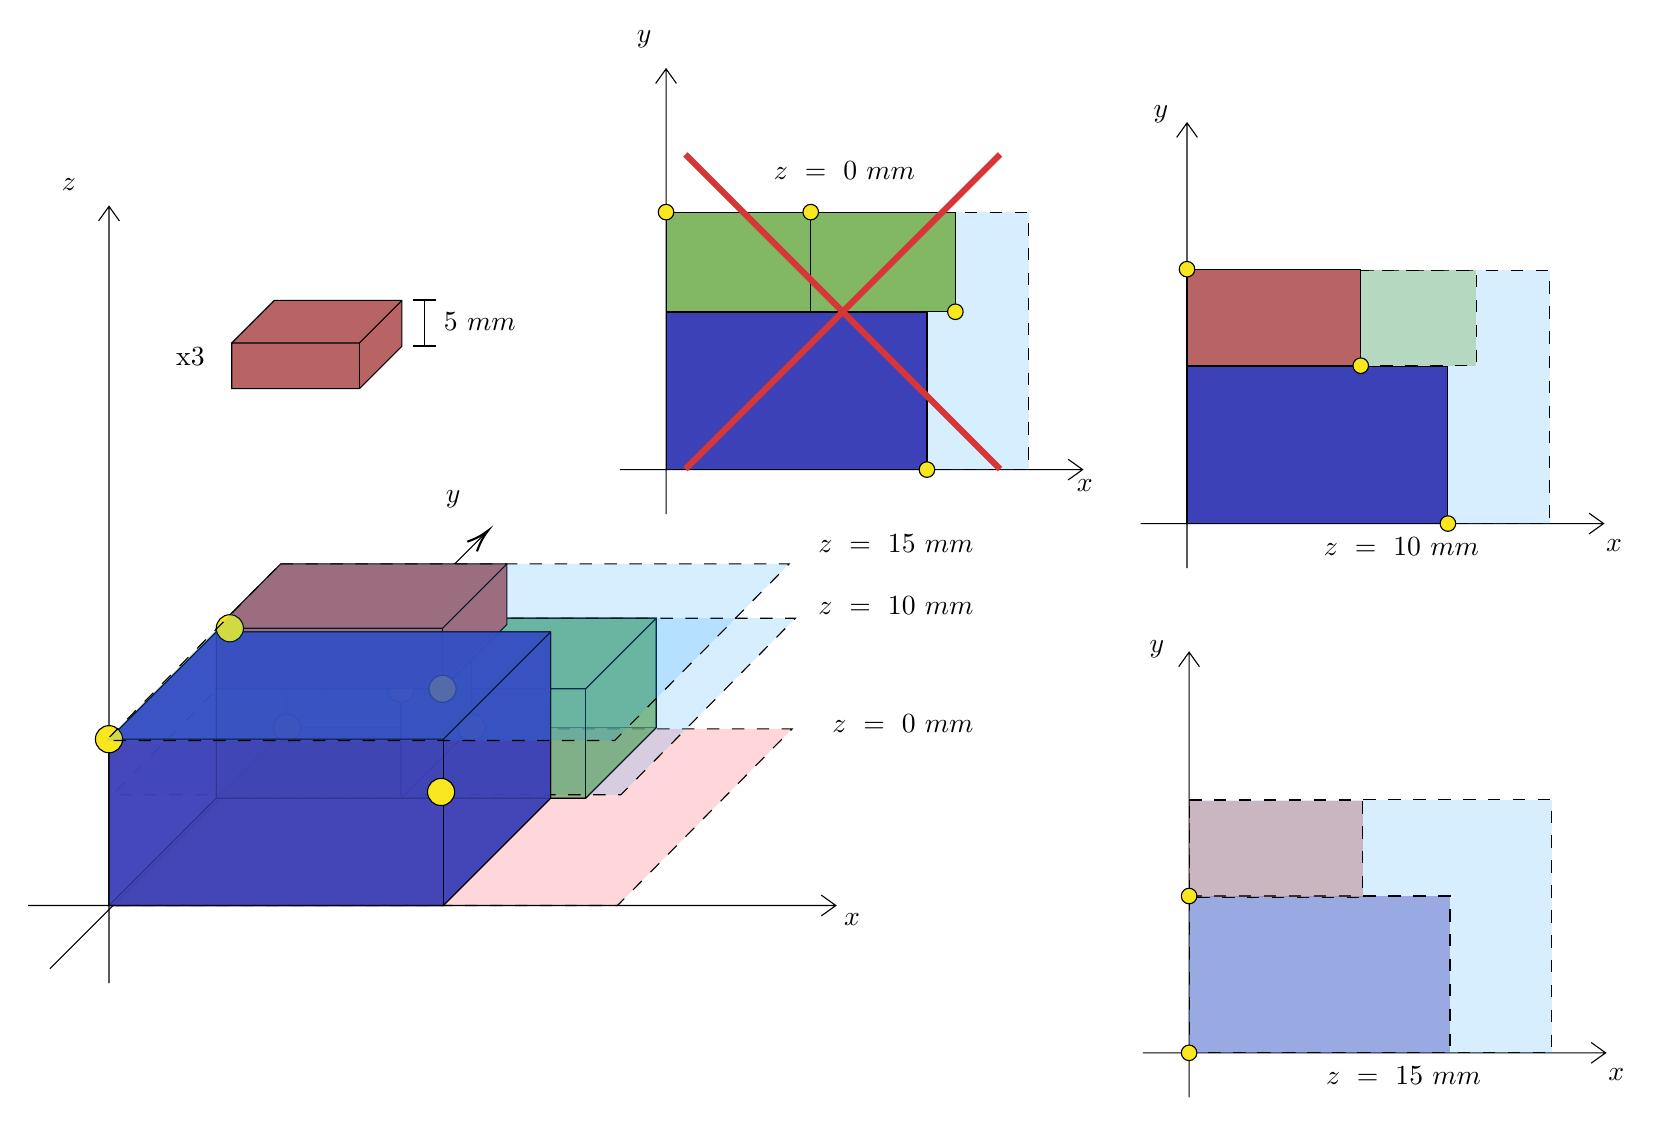
\begin{tikzpicture}[x=0.75pt,y=0.75pt,yscale=-1,xscale=1]
%uncomment if require: \path (0,537); %set diagram left start at 0, and has height of 537

%Shape: Cube [id:dp850859547377836] 
\draw  [fill={rgb, 255:red, 130; green, 184; blue, 100 }  ,fill opacity=0.63 ] (400.59,337.37) -- (366.58,371.38) -- (277.6,371.38) -- (277.6,318.66) -- (311.6,284.65) -- (400.59,284.65) -- cycle ; \draw   (277.6,371.38) -- (311.6,337.37) -- (400.59,337.37) ; \draw   (311.6,337.37) -- (311.6,284.65) ;
%Shape: Parallelogram [id:dp5823195599108398] 
\draw  [fill={rgb, 255:red, 255; green, 17; blue, 34 }  ,fill opacity=0.17 ][dash pattern={on 4.5pt off 4.5pt}] (221,338) -- (466,338) -- (381.91,423.07) -- (136.91,423.07) -- cycle ;
%Shape: Cube [id:dp46134695118901115] 
\draw  [fill={rgb, 255:red, 130; green, 184; blue, 100 }  ,fill opacity=0.63 ] (277.6,318.66) -- (311.6,284.65) -- (400.59,284.65) -- (400.59,337.37) -- (366.58,371.38) -- (277.6,371.38) -- cycle ; \draw   (400.59,284.65) -- (366.58,318.66) -- (277.6,318.66) ; \draw   (366.58,318.66) -- (366.58,371.38) ;
%Shape: Parallelogram [id:dp2915725757037321] 
\draw  [fill={rgb, 255:red, 17; green, 154; blue, 255 }  ,fill opacity=0.17 ][dash pattern={on 4.5pt off 4.5pt}] (222.62,284.65) -- (467.62,284.65) -- (383.53,369.73) -- (138.53,369.73) -- cycle ;
%Shape: Axis 2D [id:dp0385911607889563] 
\draw  (98,423.07) -- (487.11,423.07)(136.91,86.22) -- (136.91,460.5) (480.11,418.07) -- (487.11,423.07) -- (480.11,428.07) (131.91,93.22) -- (136.91,86.22) -- (141.91,93.22)  ;
%Straight Lines [id:da7790786322292883] 
\draw    (108.47,453.52) -- (318.19,243.8) ;
\draw [shift={(319.6,242.39)}, rotate = 135] [color={rgb, 255:red, 0; green, 0; blue, 0 }  ][line width=0.75]    (10.93,-3.29) .. controls (6.95,-1.4) and (3.31,-0.3) .. (0,0) .. controls (3.31,0.3) and (6.95,1.4) .. (10.93,3.29)   ;
%Shape: Cube [id:dp36816769609989985] 
\draw  [fill={rgb, 255:red, 184; green, 100; blue, 100 }  ,fill opacity=1 ] (196.05,152.05) -- (216.55,131.55) -- (278.05,131.55) -- (278.05,153.55) -- (257.55,174.05) -- (196.05,174.05) -- cycle ; \draw   (278.05,131.55) -- (257.55,152.05) -- (196.05,152.05) ; \draw   (257.55,152.05) -- (257.55,174.05) ;
%Straight Lines [id:da34140713541287426] 
\draw    (289.05,131.55) -- (289.05,153.55) ;
\draw [shift={(289.05,153.55)}, rotate = 270] [color={rgb, 255:red, 0; green, 0; blue, 0 }  ][line width=0.75]    (0,5.59) -- (0,-5.59)   ;
\draw [shift={(289.05,131.55)}, rotate = 270] [color={rgb, 255:red, 0; green, 0; blue, 0 }  ][line width=0.75]    (0,5.59) -- (0,-5.59)   ;
%Shape: Cube [id:dp46634170316063617] 
\draw  [fill={rgb, 255:red, 130; green, 184; blue, 100 }  ,fill opacity=0.63 ] (311.6,337.37) -- (277.6,371.38) -- (188.61,371.38) -- (188.61,318.66) -- (222.62,284.65) -- (311.6,284.65) -- cycle ; \draw   (188.61,371.38) -- (222.62,337.37) -- (311.6,337.37) ; \draw   (222.62,337.37) -- (222.62,284.65) ;
%Shape: Cube [id:dp7681025714248981] 
\draw  [fill={rgb, 255:red, 130; green, 184; blue, 100 }  ,fill opacity=0.63 ] (188.61,318.66) -- (222.62,284.65) -- (311.6,284.65) -- (311.6,337.37) -- (277.6,371.38) -- (188.61,371.38) -- cycle ; \draw   (311.6,284.65) -- (277.6,318.66) -- (188.61,318.66) ; \draw   (277.6,318.66) -- (277.6,371.38) ;
%Shape: Ellipse [id:dp06065829561584346] 
\draw  [fill={rgb, 255:red, 248; green, 231; blue, 28 }  ,fill opacity=1 ] (216.07,337.37) .. controls (216.07,333.75) and (219,330.82) .. (222.62,330.82) .. controls (226.23,330.82) and (229.16,333.75) .. (229.16,337.37) .. controls (229.16,340.98) and (226.23,343.91) .. (222.62,343.91) .. controls (219,343.91) and (216.07,340.98) .. (216.07,337.37) -- cycle ;
%Shape: Axis 2D [id:dp6800503914743969] 
\draw  (635,494.05) -- (858,494.05)(657.3,301) -- (657.3,515.5) (851,489.05) -- (858,494.05) -- (851,499.05) (652.3,308) -- (657.3,301) -- (662.3,308)  ;
%Shape: Rectangle [id:dp015242071789025702] 
\draw  [fill={rgb, 255:red, 17; green, 154; blue, 255 }  ,fill opacity=0.17 ][dash pattern={on 4.5pt off 4.5pt}] (657.3,372) -- (832,372) -- (832,494.05) -- (657.3,494.05) -- cycle ;
%Shape: Rectangle [id:dp1874062985177012] 
\draw  [fill={rgb, 255:red, 61; green, 65; blue, 184 }  ,fill opacity=0.4 ][dash pattern={on 4.5pt off 4.5pt}] (657.3,418.5) -- (783,418.5) -- (783,494.05) -- (657.3,494.05) -- cycle ;
%Shape: Circle [id:dp9052763715462506] 
\draw  [fill={rgb, 255:red, 248; green, 231; blue, 28 }  ,fill opacity=1 ] (653.55,494.05) .. controls (653.55,491.98) and (655.23,490.3) .. (657.3,490.3) .. controls (659.37,490.3) and (661.05,491.98) .. (661.05,494.05) .. controls (661.05,496.12) and (659.37,497.8) .. (657.3,497.8) .. controls (655.23,497.8) and (653.55,496.12) .. (653.55,494.05) -- cycle ;
%Shape: Axis 2D [id:dp6870404188341699] 
\draw  (634,239.05) -- (857,239.05)(656.3,46) -- (656.3,260.5) (850,234.05) -- (857,239.05) -- (850,244.05) (651.3,53) -- (656.3,46) -- (661.3,53)  ;
%Shape: Rectangle [id:dp3081187437769213] 
\draw  [fill={rgb, 255:red, 17; green, 154; blue, 255 }  ,fill opacity=0.17 ][dash pattern={on 4.5pt off 4.5pt}] (656.3,117) -- (831,117) -- (831,239.05) -- (656.3,239.05) -- cycle ;
%Shape: Rectangle [id:dp36934590647529786] 
\draw  [fill={rgb, 255:red, 61; green, 65; blue, 184 }  ,fill opacity=1 ] (656.3,163.5) -- (782,163.5) -- (782,239.05) -- (656.3,239.05) -- cycle ;
%Shape: Rectangle [id:dp42040004341602977] 
\draw  [fill={rgb, 255:red, 130; green, 184; blue, 100 }  ,fill opacity=0.4 ][dash pattern={on 4.5pt off 4.5pt}] (656.3,117) -- (726,117) -- (726,163) -- (656.3,163) -- cycle ;
%Shape: Circle [id:dp019789911426076] 
\draw  [fill={rgb, 255:red, 248; green, 231; blue, 28 }  ,fill opacity=1 ] (778.25,239.05) .. controls (778.25,236.98) and (779.93,235.3) .. (782,235.3) .. controls (784.07,235.3) and (785.75,236.98) .. (785.75,239.05) .. controls (785.75,241.12) and (784.07,242.8) .. (782,242.8) .. controls (779.93,242.8) and (778.25,241.12) .. (778.25,239.05) -- cycle ;
%Shape: Rectangle [id:dp7517282497666171] 
\draw  [fill={rgb, 255:red, 130; green, 184; blue, 100 }  ,fill opacity=0.4 ][dash pattern={on 4.5pt off 4.5pt}] (726,117) -- (795.7,117) -- (795.7,163) -- (726,163) -- cycle ;
%Shape: Ellipse [id:dp41816656286565723] 
\draw  [fill={rgb, 255:red, 248; green, 231; blue, 28 }  ,fill opacity=1 ] (305.06,337.37) .. controls (305.06,333.75) and (307.99,330.82) .. (311.6,330.82) .. controls (315.22,330.82) and (318.15,333.75) .. (318.15,337.37) .. controls (318.15,340.98) and (315.22,343.91) .. (311.6,343.91) .. controls (307.99,343.91) and (305.06,340.98) .. (305.06,337.37) -- cycle ;
%Shape: Ellipse [id:dp3000164568050061] 
\draw  [fill={rgb, 255:red, 248; green, 231; blue, 28 }  ,fill opacity=1 ] (271.05,318.66) .. controls (271.05,315.05) and (273.98,312.12) .. (277.6,312.12) .. controls (281.21,312.12) and (284.14,315.05) .. (284.14,318.66) .. controls (284.14,322.28) and (281.21,325.21) .. (277.6,325.21) .. controls (273.98,325.21) and (271.05,322.28) .. (271.05,318.66) -- cycle ;
%Shape: Ellipse [id:dp5080785036195841] 
\draw  [fill={rgb, 255:red, 248; green, 231; blue, 28 }  ,fill opacity=1 ] (290.37,368.37) .. controls (290.37,364.76) and (293.3,361.83) .. (296.91,361.83) .. controls (300.52,361.83) and (303.45,364.76) .. (303.45,368.37) .. controls (303.45,371.98) and (300.52,374.91) .. (296.91,374.91) .. controls (293.3,374.91) and (290.37,371.98) .. (290.37,368.37) -- cycle ;
%Shape: Cube [id:dp7940658414432213] 
\draw  [fill={rgb, 255:red, 184; green, 100; blue, 100 }  ,fill opacity=1 ] (188.61,289.5) -- (219.61,258.5) -- (328.63,258.5) -- (328.63,287.66) -- (297.63,318.66) -- (188.61,318.66) -- cycle ; \draw   (328.63,258.5) -- (297.63,289.5) -- (188.61,289.5) ; \draw   (297.63,289.5) -- (297.63,318.66) ;
%Shape: Cube [id:dp18827267498395128] 
\draw  [fill={rgb, 255:red, 61; green, 65; blue, 184 }  ,fill opacity=0.8 ] (349.7,371.38) -- (298,423.07) -- (136.91,423.07) -- (136.91,342.94) -- (188.61,291.25) -- (349.7,291.25) -- cycle ; \draw   (136.91,423.07) -- (188.61,371.38) -- (349.7,371.38) ; \draw   (188.61,371.38) -- (188.61,291.25) ;
%Shape: Ellipse [id:dp46823065251729934] 
\draw  [fill={rgb, 255:red, 248; green, 231; blue, 28 }  ,fill opacity=1 ] (291.09,318.66) .. controls (291.09,315.05) and (294.02,312.12) .. (297.63,312.12) .. controls (301.24,312.12) and (304.17,315.05) .. (304.17,318.66) .. controls (304.17,322.28) and (301.24,325.21) .. (297.63,325.21) .. controls (294.02,325.21) and (291.09,322.28) .. (291.09,318.66) -- cycle ;
%Shape: Cube [id:dp6823756616236724] 
\draw  [fill={rgb, 255:red, 61; green, 65; blue, 184 }  ,fill opacity=0.8 ] (136.91,342.94) -- (188.61,291.25) -- (349.7,291.25) -- (349.7,371.38) -- (298,423.07) -- (136.91,423.07) -- cycle ; \draw   (349.7,291.25) -- (298,342.94) -- (136.91,342.94) ; \draw   (298,342.94) -- (298,423.07) ;
%Shape: Ellipse [id:dp5738431884006834] 
\draw  [fill={rgb, 255:red, 248; green, 231; blue, 28 }  ,fill opacity=1 ] (130.37,342.94) .. controls (130.37,339.33) and (133.3,336.4) .. (136.91,336.4) .. controls (140.52,336.4) and (143.45,339.33) .. (143.45,342.94) .. controls (143.45,346.56) and (140.52,349.49) .. (136.91,349.49) .. controls (133.3,349.49) and (130.37,346.56) .. (130.37,342.94) -- cycle ;
%Shape: Ellipse [id:dp07646261428683299] 
\draw  [fill={rgb, 255:red, 248; green, 231; blue, 28 }  ,fill opacity=1 ] (188.61,289.5) .. controls (188.61,285.89) and (191.54,282.96) .. (195.15,282.96) .. controls (198.77,282.96) and (201.69,285.89) .. (201.69,289.5) .. controls (201.69,293.11) and (198.77,296.04) .. (195.15,296.04) .. controls (191.54,296.04) and (188.61,293.11) .. (188.61,289.5) -- cycle ;
%Shape: Parallelogram [id:dp08950497007303859] 
\draw  [fill={rgb, 255:red, 17; green, 154; blue, 255 }  ,fill opacity=0.17 ][dash pattern={on 4.5pt off 4.5pt}] (219.61,258.5) -- (464.61,258.5) -- (380.52,343.57) -- (135.52,343.57) -- cycle ;
%Shape: Rectangle [id:dp4478205527448239] 
\draw  [fill={rgb, 255:red, 184; green, 100; blue, 100 }  ,fill opacity=1 ] (656.3,116.5) -- (740,116.5) -- (740,163) -- (656.3,163) -- cycle ;
%Shape: Circle [id:dp13454299239933898] 
\draw  [fill={rgb, 255:red, 248; green, 231; blue, 28 }  ,fill opacity=1 ] (736.25,163) .. controls (736.25,160.93) and (737.93,159.25) .. (740,159.25) .. controls (742.07,159.25) and (743.75,160.93) .. (743.75,163) .. controls (743.75,165.07) and (742.07,166.75) .. (740,166.75) .. controls (737.93,166.75) and (736.25,165.07) .. (736.25,163) -- cycle ;
%Shape: Circle [id:dp8773584456012923] 
\draw  [fill={rgb, 255:red, 248; green, 231; blue, 28 }  ,fill opacity=1 ] (652.55,116.5) .. controls (652.55,114.43) and (654.23,112.75) .. (656.3,112.75) .. controls (658.37,112.75) and (660.05,114.43) .. (660.05,116.5) .. controls (660.05,118.57) and (658.37,120.25) .. (656.3,120.25) .. controls (654.23,120.25) and (652.55,118.57) .. (652.55,116.5) -- cycle ;
%Shape: Rectangle [id:dp6527670874867769] 
\draw  [fill={rgb, 255:red, 184; green, 100; blue, 100 }  ,fill opacity=0.4 ][dash pattern={on 4.5pt off 4.5pt}] (657.3,372.5) -- (741,372.5) -- (741,419) -- (657.3,419) -- cycle ;
%Shape: Circle [id:dp2657813756631938] 
\draw  [fill={rgb, 255:red, 248; green, 231; blue, 28 }  ,fill opacity=1 ] (653.55,418.5) .. controls (653.55,416.43) and (655.23,414.75) .. (657.3,414.75) .. controls (659.37,414.75) and (661.05,416.43) .. (661.05,418.5) .. controls (661.05,420.57) and (659.37,422.25) .. (657.3,422.25) .. controls (655.23,422.25) and (653.55,420.57) .. (653.55,418.5) -- cycle ;
%Shape: Ellipse [id:dp22740515272810635] 
\draw  [fill={rgb, 255:red, 248; green, 231; blue, 28 }  ,fill opacity=1 ] (290.37,368.37) .. controls (290.37,364.76) and (293.3,361.83) .. (296.91,361.83) .. controls (300.52,361.83) and (303.45,364.76) .. (303.45,368.37) .. controls (303.45,371.98) and (300.52,374.91) .. (296.91,374.91) .. controls (293.3,374.91) and (290.37,371.98) .. (290.37,368.37) -- cycle ;
%Shape: Axis 2D [id:dp28534705658973836] 
\draw  (383,213.05) -- (606,213.05)(405.3,20) -- (405.3,234.5) (599,208.05) -- (606,213.05) -- (599,218.05) (400.3,27) -- (405.3,20) -- (410.3,27)  ;
%Shape: Rectangle [id:dp34444980481385135] 
\draw  [fill={rgb, 255:red, 17; green, 154; blue, 255 }  ,fill opacity=0.17 ][dash pattern={on 4.5pt off 4.5pt}] (405.3,89) -- (580,89) -- (580,213.05) -- (405.3,213.05) -- cycle ;
%Shape: Rectangle [id:dp6600565254726414] 
\draw  [fill={rgb, 255:red, 61; green, 65; blue, 184 }  ,fill opacity=1 ] (405.3,137.5) -- (531,137.5) -- (531,213.05) -- (405.3,213.05) -- cycle ;
%Shape: Circle [id:dp687328768761151] 
\draw  [fill={rgb, 255:red, 248; green, 231; blue, 28 }  ,fill opacity=1 ] (527.25,213.05) .. controls (527.25,210.98) and (528.93,209.3) .. (531,209.3) .. controls (533.07,209.3) and (534.75,210.98) .. (534.75,213.05) .. controls (534.75,215.12) and (533.07,216.8) .. (531,216.8) .. controls (528.93,216.8) and (527.25,215.12) .. (527.25,213.05) -- cycle ;
%Shape: Rectangle [id:dp4720998169870536] 
\draw  [fill={rgb, 255:red, 130; green, 184; blue, 100 }  ,fill opacity=1 ] (405.3,89) -- (475,89) -- (475,137) -- (405.3,137) -- cycle ;
%Shape: Circle [id:dp2451407265899025] 
\draw  [fill={rgb, 255:red, 248; green, 231; blue, 28 }  ,fill opacity=1 ] (401.55,89) .. controls (401.55,86.93) and (403.23,85.25) .. (405.3,85.25) .. controls (407.37,85.25) and (409.05,86.93) .. (409.05,89) .. controls (409.05,91.07) and (407.37,92.75) .. (405.3,92.75) .. controls (403.23,92.75) and (401.55,91.07) .. (401.55,89) -- cycle ;
%Shape: Rectangle [id:dp9804240171062975] 
\draw  [fill={rgb, 255:red, 130; green, 184; blue, 100 }  ,fill opacity=1 ] (475,89) -- (544.7,89) -- (544.7,137) -- (475,137) -- cycle ;
%Shape: Circle [id:dp3092275472196101] 
\draw  [fill={rgb, 255:red, 248; green, 231; blue, 28 }  ,fill opacity=1 ] (540.95,137) .. controls (540.95,134.93) and (542.63,133.25) .. (544.7,133.25) .. controls (546.77,133.25) and (548.45,134.93) .. (548.45,137) .. controls (548.45,139.07) and (546.77,140.75) .. (544.7,140.75) .. controls (542.63,140.75) and (540.95,139.07) .. (540.95,137) -- cycle ;
%Shape: Circle [id:dp07506811257370083] 
\draw  [fill={rgb, 255:red, 248; green, 231; blue, 28 }  ,fill opacity=1 ] (471.25,89) .. controls (471.25,86.93) and (472.93,85.25) .. (475,85.25) .. controls (477.07,85.25) and (478.75,86.93) .. (478.75,89) .. controls (478.75,91.07) and (477.07,92.75) .. (475,92.75) .. controls (472.93,92.75) and (471.25,91.07) .. (471.25,89) -- cycle ;
\draw  [color={rgb, 255:red, 214; green, 54; blue, 54 }  ,draw opacity=1 ][line width=2.25]  (414.59,61.2) -- (566.2,212.8)(566.2,61.2) -- (414.59,212.8) ;

% Text Node
\draw (484.19,329.66) node [anchor=north west][inner sep=0.75pt]    {$z\ =\ 0\ mm$};
% Text Node
\draw (297.9,221.7) node [anchor=north west][inner sep=0.75pt]    {$y$};
% Text Node
\draw (489.84,425.85) node [anchor=north west][inner sep=0.75pt]    {$x$};
% Text Node
\draw (112.94,71.64) node [anchor=north west][inner sep=0.75pt]    {$z$};
% Text Node
\draw (168,153) node [anchor=north west][inner sep=0.75pt]   [align=left] {x3};
% Text Node
\draw (297.05,135.95) node [anchor=north west][inner sep=0.75pt]    {$5\ mm$};
% Text Node
\draw (477.48,243.2) node [anchor=north west][inner sep=0.75pt]    {$z\ =\ 15\ mm$};
% Text Node
\draw (858,500.4) node [anchor=north west][inner sep=0.75pt]    {$x$};
% Text Node
\draw (639,36.4) node [anchor=north west][inner sep=0.75pt]    {$y$};
% Text Node
\draw (722,499.4) node [anchor=north west][inner sep=0.75pt]    {$z\ =\ 15\ mm$};
% Text Node
\draw (477.48,273.2) node [anchor=north west][inner sep=0.75pt]    {$z\ =\ 10\ mm$};
% Text Node
\draw (857,245.4) node [anchor=north west][inner sep=0.75pt]    {$x$};
% Text Node
\draw (721,244.4) node [anchor=north west][inner sep=0.75pt]    {$z\ =\ 10\ mm$};
% Text Node
\draw (390,0.4) node [anchor=north west][inner sep=0.75pt]    {$y$};
% Text Node
\draw (456,63.4) node [anchor=north west][inner sep=0.75pt]    {$z\ =\ 0\ mm$};
% Text Node
\draw (637,294.4) node [anchor=north west][inner sep=0.75pt]    {$y$};
% Text Node
\draw (602,216.4) node [anchor=north west][inner sep=0.75pt]    {$x$};


\end{tikzpicture}

            }
        \end{figure}
    \end{frame}
    \begin{frame}{Support Planes}
        \begin{figure}[h]
            \resizebox*{!}{65mm}{%
            

\tikzset{every picture/.style={line width=0.75pt}} %set default line width to 0.75pt        

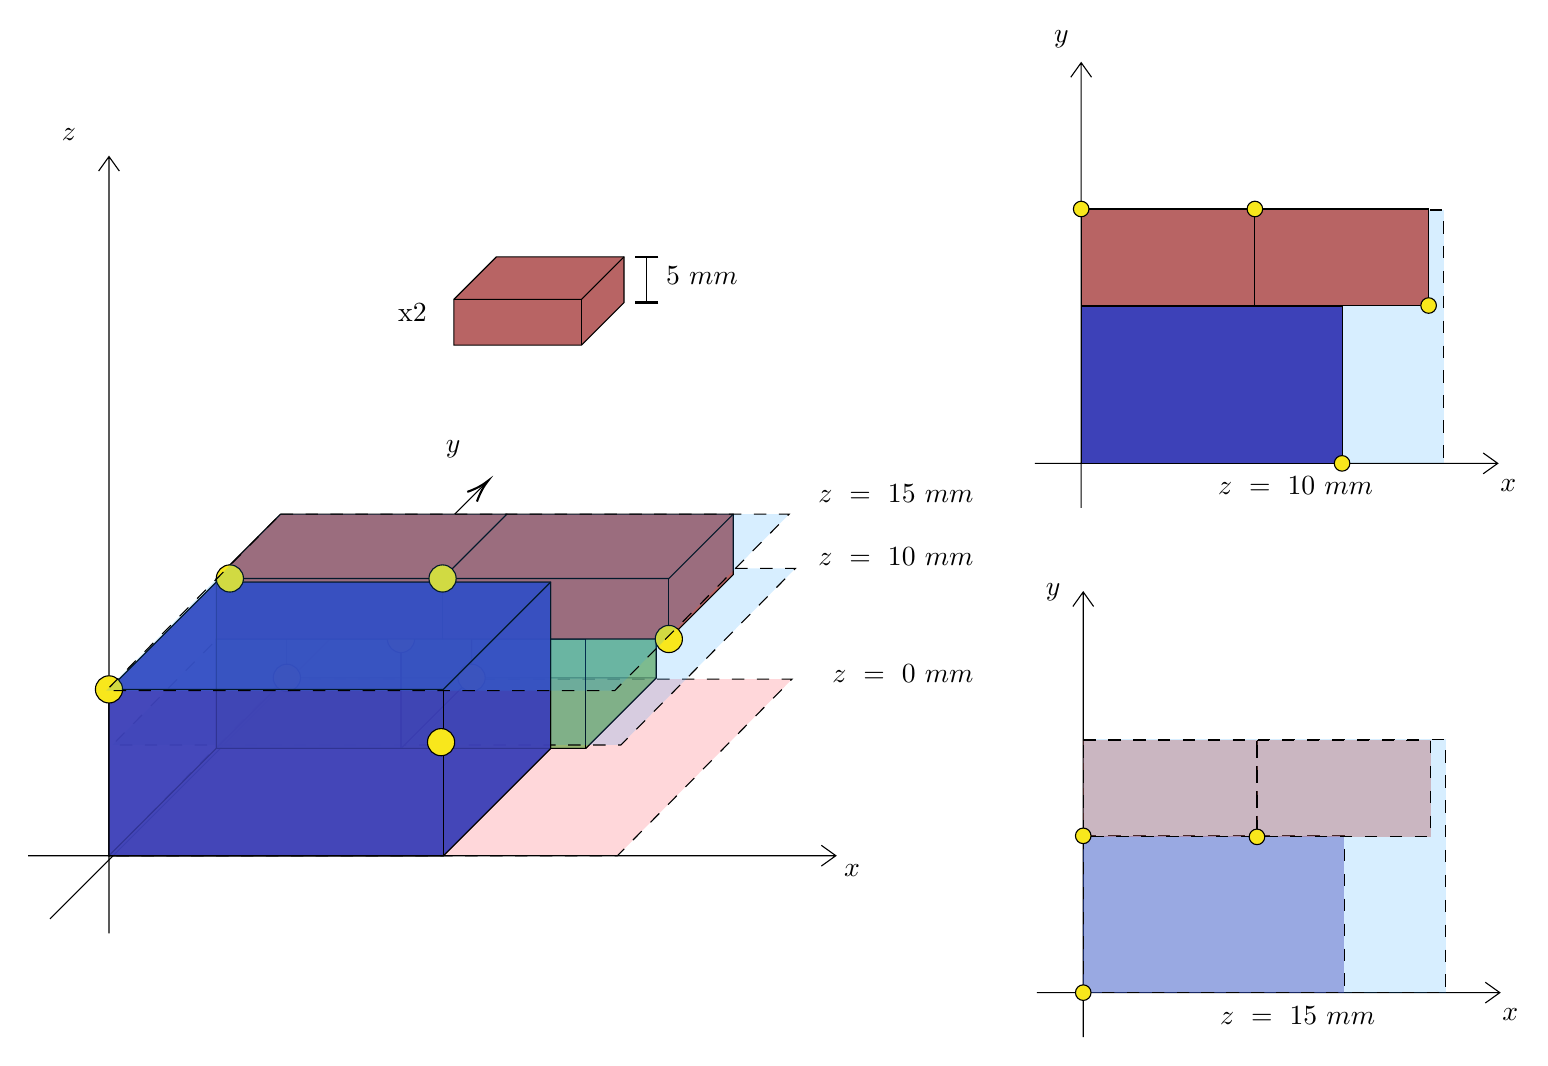
\begin{tikzpicture}[x=0.75pt,y=0.75pt,yscale=-1,xscale=1]
%uncomment if require: \path (0,536); %set diagram left start at 0, and has height of 536

%Shape: Cube [id:dp24118624821606238] 
\draw  [fill={rgb, 255:red, 130; green, 184; blue, 100 }  ,fill opacity=0.63 ] (380.59,330.87) -- (346.58,364.88) -- (257.6,364.88) -- (257.6,312.16) -- (291.6,278.15) -- (380.59,278.15) -- cycle ; \draw   (257.6,364.88) -- (291.6,330.87) -- (380.59,330.87) ; \draw   (291.6,330.87) -- (291.6,278.15) ;
%Shape: Parallelogram [id:dp818489623347525] 
\draw  [fill={rgb, 255:red, 255; green, 17; blue, 34 }  ,fill opacity=0.17 ][dash pattern={on 4.5pt off 4.5pt}] (201,331.5) -- (446,331.5) -- (361.91,416.57) -- (116.91,416.57) -- cycle ;
%Shape: Cube [id:dp029725286983864785] 
\draw  [fill={rgb, 255:red, 130; green, 184; blue, 100 }  ,fill opacity=0.63 ] (257.6,312.16) -- (291.6,278.15) -- (380.59,278.15) -- (380.59,330.87) -- (346.58,364.88) -- (257.6,364.88) -- cycle ; \draw   (380.59,278.15) -- (346.58,312.16) -- (257.6,312.16) ; \draw   (346.58,312.16) -- (346.58,364.88) ;
%Shape: Parallelogram [id:dp33144149017282] 
\draw  [fill={rgb, 255:red, 17; green, 154; blue, 255 }  ,fill opacity=0.17 ][dash pattern={on 4.5pt off 4.5pt}] (202.62,278.15) -- (447.62,278.15) -- (363.53,363.23) -- (118.53,363.23) -- cycle ;
%Shape: Axis 2D [id:dp7280305968897177] 
\draw  (78,416.57) -- (467.11,416.57)(116.91,79.72) -- (116.91,454) (460.11,411.57) -- (467.11,416.57) -- (460.11,421.57) (111.91,86.72) -- (116.91,79.72) -- (121.91,86.72)  ;
%Straight Lines [id:da37913853440794043] 
\draw    (88.47,447.02) -- (298.19,237.3) ;
\draw [shift={(299.6,235.89)}, rotate = 135] [color={rgb, 255:red, 0; green, 0; blue, 0 }  ][line width=0.75]    (10.93,-3.29) .. controls (6.95,-1.4) and (3.31,-0.3) .. (0,0) .. controls (3.31,0.3) and (6.95,1.4) .. (10.93,3.29)   ;
%Shape: Cube [id:dp43786688235829296] 
\draw  [fill={rgb, 255:red, 184; green, 100; blue, 100 }  ,fill opacity=1 ] (283.05,148.55) -- (303.55,128.05) -- (365.05,128.05) -- (365.05,150.05) -- (344.55,170.55) -- (283.05,170.55) -- cycle ; \draw   (365.05,128.05) -- (344.55,148.55) -- (283.05,148.55) ; \draw   (344.55,148.55) -- (344.55,170.55) ;
%Straight Lines [id:da5152098563828622] 
\draw    (376.05,128.05) -- (376.05,150.05) ;
\draw [shift={(376.05,150.05)}, rotate = 270] [color={rgb, 255:red, 0; green, 0; blue, 0 }  ][line width=0.75]    (0,5.59) -- (0,-5.59)   ;
\draw [shift={(376.05,128.05)}, rotate = 270] [color={rgb, 255:red, 0; green, 0; blue, 0 }  ][line width=0.75]    (0,5.59) -- (0,-5.59)   ;
%Shape: Cube [id:dp44715071573908904] 
\draw  [fill={rgb, 255:red, 130; green, 184; blue, 100 }  ,fill opacity=0.63 ] (291.6,330.87) -- (257.6,364.88) -- (168.61,364.88) -- (168.61,312.16) -- (202.62,278.15) -- (291.6,278.15) -- cycle ; \draw   (168.61,364.88) -- (202.62,330.87) -- (291.6,330.87) ; \draw   (202.62,330.87) -- (202.62,278.15) ;
%Shape: Cube [id:dp4497792783120459] 
\draw  [fill={rgb, 255:red, 130; green, 184; blue, 100 }  ,fill opacity=0.63 ] (168.61,312.16) -- (202.62,278.15) -- (291.6,278.15) -- (291.6,330.87) -- (257.6,364.88) -- (168.61,364.88) -- cycle ; \draw   (291.6,278.15) -- (257.6,312.16) -- (168.61,312.16) ; \draw   (257.6,312.16) -- (257.6,364.88) ;
%Shape: Ellipse [id:dp8025395959106266] 
\draw  [fill={rgb, 255:red, 248; green, 231; blue, 28 }  ,fill opacity=1 ] (196.07,330.87) .. controls (196.07,327.25) and (199,324.32) .. (202.62,324.32) .. controls (206.23,324.32) and (209.16,327.25) .. (209.16,330.87) .. controls (209.16,334.48) and (206.23,337.41) .. (202.62,337.41) .. controls (199,337.41) and (196.07,334.48) .. (196.07,330.87) -- cycle ;
%Shape: Axis 2D [id:dp6262269767988246] 
\draw  (564,482.55) -- (787,482.55)(586.3,289.5) -- (586.3,504) (780,477.55) -- (787,482.55) -- (780,487.55) (581.3,296.5) -- (586.3,289.5) -- (591.3,296.5)  ;
%Shape: Rectangle [id:dp7104361292217809] 
\draw  [fill={rgb, 255:red, 17; green, 154; blue, 255 }  ,fill opacity=0.17 ][dash pattern={on 4.5pt off 4.5pt}] (586.3,360.5) -- (761,360.5) -- (761,482.55) -- (586.3,482.55) -- cycle ;
%Shape: Rectangle [id:dp4551089431649423] 
\draw  [fill={rgb, 255:red, 61; green, 65; blue, 184 }  ,fill opacity=0.4 ][dash pattern={on 4.5pt off 4.5pt}] (586.3,407) -- (712,407) -- (712,482.55) -- (586.3,482.55) -- cycle ;
%Shape: Circle [id:dp4624770541343133] 
\draw  [fill={rgb, 255:red, 248; green, 231; blue, 28 }  ,fill opacity=1 ] (582.55,482.55) .. controls (582.55,480.48) and (584.23,478.8) .. (586.3,478.8) .. controls (588.37,478.8) and (590.05,480.48) .. (590.05,482.55) .. controls (590.05,484.62) and (588.37,486.3) .. (586.3,486.3) .. controls (584.23,486.3) and (582.55,484.62) .. (582.55,482.55) -- cycle ;
%Shape: Axis 2D [id:dp969470029295066] 
\draw  (563,227.55) -- (786,227.55)(585.3,34.5) -- (585.3,249) (779,222.55) -- (786,227.55) -- (779,232.55) (580.3,41.5) -- (585.3,34.5) -- (590.3,41.5)  ;
%Shape: Rectangle [id:dp4261055316386787] 
\draw  [fill={rgb, 255:red, 17; green, 154; blue, 255 }  ,fill opacity=0.17 ][dash pattern={on 4.5pt off 4.5pt}] (585.3,105.5) -- (760,105.5) -- (760,227.55) -- (585.3,227.55) -- cycle ;
%Shape: Rectangle [id:dp5378646202813674] 
\draw  [fill={rgb, 255:red, 61; green, 65; blue, 184 }  ,fill opacity=1 ] (585.3,152) -- (711,152) -- (711,227.55) -- (585.3,227.55) -- cycle ;
%Shape: Rectangle [id:dp8852671695477923] 
\draw  [fill={rgb, 255:red, 130; green, 184; blue, 100 }  ,fill opacity=0.4 ][dash pattern={on 4.5pt off 4.5pt}] (585.3,105.5) -- (655,105.5) -- (655,151.5) -- (585.3,151.5) -- cycle ;
%Shape: Circle [id:dp2270367067514596] 
\draw  [fill={rgb, 255:red, 248; green, 231; blue, 28 }  ,fill opacity=1 ] (707.25,227.55) .. controls (707.25,225.48) and (708.93,223.8) .. (711,223.8) .. controls (713.07,223.8) and (714.75,225.48) .. (714.75,227.55) .. controls (714.75,229.62) and (713.07,231.3) .. (711,231.3) .. controls (708.93,231.3) and (707.25,229.62) .. (707.25,227.55) -- cycle ;
%Shape: Rectangle [id:dp681624257096331] 
\draw  [fill={rgb, 255:red, 130; green, 184; blue, 100 }  ,fill opacity=0.4 ][dash pattern={on 4.5pt off 4.5pt}] (655,105.5) -- (724.7,105.5) -- (724.7,151.5) -- (655,151.5) -- cycle ;
%Shape: Ellipse [id:dp4533387898963953] 
\draw  [fill={rgb, 255:red, 248; green, 231; blue, 28 }  ,fill opacity=1 ] (285.06,330.87) .. controls (285.06,327.25) and (287.99,324.32) .. (291.6,324.32) .. controls (295.22,324.32) and (298.15,327.25) .. (298.15,330.87) .. controls (298.15,334.48) and (295.22,337.41) .. (291.6,337.41) .. controls (287.99,337.41) and (285.06,334.48) .. (285.06,330.87) -- cycle ;
%Shape: Ellipse [id:dp2258337282012488] 
\draw  [fill={rgb, 255:red, 248; green, 231; blue, 28 }  ,fill opacity=1 ] (251.05,312.16) .. controls (251.05,308.55) and (253.98,305.62) .. (257.6,305.62) .. controls (261.21,305.62) and (264.14,308.55) .. (264.14,312.16) .. controls (264.14,315.78) and (261.21,318.71) .. (257.6,318.71) .. controls (253.98,318.71) and (251.05,315.78) .. (251.05,312.16) -- cycle ;
%Shape: Ellipse [id:dp6988819335078928] 
\draw  [fill={rgb, 255:red, 248; green, 231; blue, 28 }  ,fill opacity=1 ] (270.37,361.87) .. controls (270.37,358.26) and (273.3,355.33) .. (276.91,355.33) .. controls (280.52,355.33) and (283.45,358.26) .. (283.45,361.87) .. controls (283.45,365.48) and (280.52,368.41) .. (276.91,368.41) .. controls (273.3,368.41) and (270.37,365.48) .. (270.37,361.87) -- cycle ;
%Shape: Cube [id:dp7385806895005637] 
\draw  [fill={rgb, 255:red, 184; green, 100; blue, 100 }  ,fill opacity=1 ] (168.61,283) -- (199.61,252) -- (308.63,252) -- (308.63,281.16) -- (277.63,312.16) -- (168.61,312.16) -- cycle ; \draw   (308.63,252) -- (277.63,283) -- (168.61,283) ; \draw   (277.63,283) -- (277.63,312.16) ;
%Shape: Cube [id:dp46845990607049726] 
\draw  [fill={rgb, 255:red, 184; green, 100; blue, 100 }  ,fill opacity=1 ] (277.63,283) -- (308.63,252) -- (417.65,252) -- (417.65,281.16) -- (386.65,312.16) -- (277.63,312.16) -- cycle ; \draw   (417.65,252) -- (386.65,283) -- (277.63,283) ; \draw   (386.65,283) -- (386.65,312.16) ;
%Shape: Cube [id:dp038868241472426956] 
\draw  [fill={rgb, 255:red, 61; green, 65; blue, 184 }  ,fill opacity=0.8 ] (329.7,364.88) -- (278,416.57) -- (116.91,416.57) -- (116.91,336.44) -- (168.61,284.75) -- (329.7,284.75) -- cycle ; \draw   (116.91,416.57) -- (168.61,364.88) -- (329.7,364.88) ; \draw   (168.61,364.88) -- (168.61,284.75) ;
%Shape: Ellipse [id:dp17174095369862896] 
\draw  [fill={rgb, 255:red, 248; green, 231; blue, 28 }  ,fill opacity=1 ] (380.11,312.16) .. controls (380.11,308.55) and (383.04,305.62) .. (386.65,305.62) .. controls (390.26,305.62) and (393.19,308.55) .. (393.19,312.16) .. controls (393.19,315.78) and (390.26,318.71) .. (386.65,318.71) .. controls (383.04,318.71) and (380.11,315.78) .. (380.11,312.16) -- cycle ;
%Shape: Cube [id:dp7592145851564649] 
\draw  [fill={rgb, 255:red, 61; green, 65; blue, 184 }  ,fill opacity=0.8 ] (116.91,336.44) -- (168.61,284.75) -- (329.7,284.75) -- (329.7,364.88) -- (278,416.57) -- (116.91,416.57) -- cycle ; \draw   (329.7,284.75) -- (278,336.44) -- (116.91,336.44) ; \draw   (278,336.44) -- (278,416.57) ;
%Shape: Ellipse [id:dp7845489096437979] 
\draw  [fill={rgb, 255:red, 248; green, 231; blue, 28 }  ,fill opacity=1 ] (110.37,336.44) .. controls (110.37,332.83) and (113.3,329.9) .. (116.91,329.9) .. controls (120.52,329.9) and (123.45,332.83) .. (123.45,336.44) .. controls (123.45,340.06) and (120.52,342.99) .. (116.91,342.99) .. controls (113.3,342.99) and (110.37,340.06) .. (110.37,336.44) -- cycle ;
%Shape: Ellipse [id:dp13625248726647632] 
\draw  [fill={rgb, 255:red, 248; green, 231; blue, 28 }  ,fill opacity=1 ] (168.61,283) .. controls (168.61,279.39) and (171.54,276.46) .. (175.15,276.46) .. controls (178.77,276.46) and (181.69,279.39) .. (181.69,283) .. controls (181.69,286.61) and (178.77,289.54) .. (175.15,289.54) .. controls (171.54,289.54) and (168.61,286.61) .. (168.61,283) -- cycle ;
%Shape: Ellipse [id:dp22786020311457056] 
\draw  [fill={rgb, 255:red, 248; green, 231; blue, 28 }  ,fill opacity=1 ] (271.09,283) .. controls (271.09,279.39) and (274.02,276.46) .. (277.63,276.46) .. controls (281.24,276.46) and (284.17,279.39) .. (284.17,283) .. controls (284.17,286.61) and (281.24,289.54) .. (277.63,289.54) .. controls (274.02,289.54) and (271.09,286.61) .. (271.09,283) -- cycle ;
%Shape: Parallelogram [id:dp2697731816540232] 
\draw  [fill={rgb, 255:red, 17; green, 154; blue, 255 }  ,fill opacity=0.17 ][dash pattern={on 4.5pt off 4.5pt}] (199.61,252) -- (444.61,252) -- (360.52,337.07) -- (115.52,337.07) -- cycle ;
%Shape: Rectangle [id:dp5173633377498139] 
\draw  [fill={rgb, 255:red, 184; green, 100; blue, 100 }  ,fill opacity=1 ] (585.3,105) -- (669,105) -- (669,151.5) -- (585.3,151.5) -- cycle ;
%Shape: Rectangle [id:dp6123569401126313] 
\draw  [fill={rgb, 255:red, 184; green, 100; blue, 100 }  ,fill opacity=1 ] (669,105) -- (752.7,105) -- (752.7,151.5) -- (669,151.5) -- cycle ;
%Shape: Circle [id:dp24876807610289275] 
\draw  [fill={rgb, 255:red, 248; green, 231; blue, 28 }  ,fill opacity=1 ] (748.95,151.5) .. controls (748.95,149.43) and (750.63,147.75) .. (752.7,147.75) .. controls (754.77,147.75) and (756.45,149.43) .. (756.45,151.5) .. controls (756.45,153.57) and (754.77,155.25) .. (752.7,155.25) .. controls (750.63,155.25) and (748.95,153.57) .. (748.95,151.5) -- cycle ;
%Shape: Circle [id:dp5040183450074549] 
\draw  [fill={rgb, 255:red, 248; green, 231; blue, 28 }  ,fill opacity=1 ] (665.25,105) .. controls (665.25,102.93) and (666.93,101.25) .. (669,101.25) .. controls (671.07,101.25) and (672.75,102.93) .. (672.75,105) .. controls (672.75,107.07) and (671.07,108.75) .. (669,108.75) .. controls (666.93,108.75) and (665.25,107.07) .. (665.25,105) -- cycle ;
%Shape: Circle [id:dp15069165887500435] 
\draw  [fill={rgb, 255:red, 248; green, 231; blue, 28 }  ,fill opacity=1 ] (581.55,105) .. controls (581.55,102.93) and (583.23,101.25) .. (585.3,101.25) .. controls (587.37,101.25) and (589.05,102.93) .. (589.05,105) .. controls (589.05,107.07) and (587.37,108.75) .. (585.3,108.75) .. controls (583.23,108.75) and (581.55,107.07) .. (581.55,105) -- cycle ;
%Shape: Rectangle [id:dp7396378678302288] 
\draw  [fill={rgb, 255:red, 184; green, 100; blue, 100 }  ,fill opacity=0.4 ][dash pattern={on 4.5pt off 4.5pt}] (586.3,361) -- (670,361) -- (670,407.5) -- (586.3,407.5) -- cycle ;
%Shape: Rectangle [id:dp5053870797116731] 
\draw  [fill={rgb, 255:red, 184; green, 100; blue, 100 }  ,fill opacity=0.4 ][dash pattern={on 4.5pt off 4.5pt}] (670,361) -- (753.7,361) -- (753.7,407.5) -- (670,407.5) -- cycle ;
%Shape: Circle [id:dp5616704740283756] 
\draw  [fill={rgb, 255:red, 248; green, 231; blue, 28 }  ,fill opacity=1 ] (582.55,407) .. controls (582.55,404.93) and (584.23,403.25) .. (586.3,403.25) .. controls (588.37,403.25) and (590.05,404.93) .. (590.05,407) .. controls (590.05,409.07) and (588.37,410.75) .. (586.3,410.75) .. controls (584.23,410.75) and (582.55,409.07) .. (582.55,407) -- cycle ;
%Shape: Circle [id:dp2597410649320595] 
\draw  [fill={rgb, 255:red, 248; green, 231; blue, 28 }  ,fill opacity=1 ] (666.25,407.5) .. controls (666.25,405.43) and (667.93,403.75) .. (670,403.75) .. controls (672.07,403.75) and (673.75,405.43) .. (673.75,407.5) .. controls (673.75,409.57) and (672.07,411.25) .. (670,411.25) .. controls (667.93,411.25) and (666.25,409.57) .. (666.25,407.5) -- cycle ;
%Shape: Ellipse [id:dp5241097716779531] 
\draw  [fill={rgb, 255:red, 248; green, 231; blue, 28 }  ,fill opacity=1 ] (270.37,361.87) .. controls (270.37,358.26) and (273.3,355.33) .. (276.91,355.33) .. controls (280.52,355.33) and (283.45,358.26) .. (283.45,361.87) .. controls (283.45,365.48) and (280.52,368.41) .. (276.91,368.41) .. controls (273.3,368.41) and (270.37,365.48) .. (270.37,361.87) -- cycle ;

% Text Node
\draw (464.19,323.16) node [anchor=north west][inner sep=0.75pt]    {$z\ =\ 0\ mm$};
% Text Node
\draw (277.9,215.2) node [anchor=north west][inner sep=0.75pt]    {$y$};
% Text Node
\draw (469.84,419.35) node [anchor=north west][inner sep=0.75pt]    {$x$};
% Text Node
\draw (92.94,65.14) node [anchor=north west][inner sep=0.75pt]    {$z$};
% Text Node
\draw (255,149.5) node [anchor=north west][inner sep=0.75pt]   [align=left] {x2};
% Text Node
\draw (384.05,131.45) node [anchor=north west][inner sep=0.75pt]    {$5\ mm$};
% Text Node
\draw (457.48,236.7) node [anchor=north west][inner sep=0.75pt]    {$z\ =\ 15\ mm$};
% Text Node
\draw (787,488.9) node [anchor=north west][inner sep=0.75pt]    {$x$};
% Text Node
\draw (571,17.9) node [anchor=north west][inner sep=0.75pt]    {$y$};
% Text Node
\draw (651,487.9) node [anchor=north west][inner sep=0.75pt]    {$z\ =\ 15\ mm$};
% Text Node
\draw (457.48,266.7) node [anchor=north west][inner sep=0.75pt]    {$z\ =\ 10\ mm$};
% Text Node
\draw (786,233.9) node [anchor=north west][inner sep=0.75pt]    {$x$};
% Text Node
\draw (650,232.9) node [anchor=north west][inner sep=0.75pt]    {$z\ =\ 10\ mm$};
% Text Node
\draw (567,284.4) node [anchor=north west][inner sep=0.75pt]    {$y$};


\end{tikzpicture}

            }
        \end{figure}
    \end{frame}
    \begin{frame}{Support Planes}
        \begin{figure}[h]
            \resizebox*{!}{65mm}{%
            

\tikzset{every picture/.style={line width=0.75pt}} %set default line width to 0.75pt        

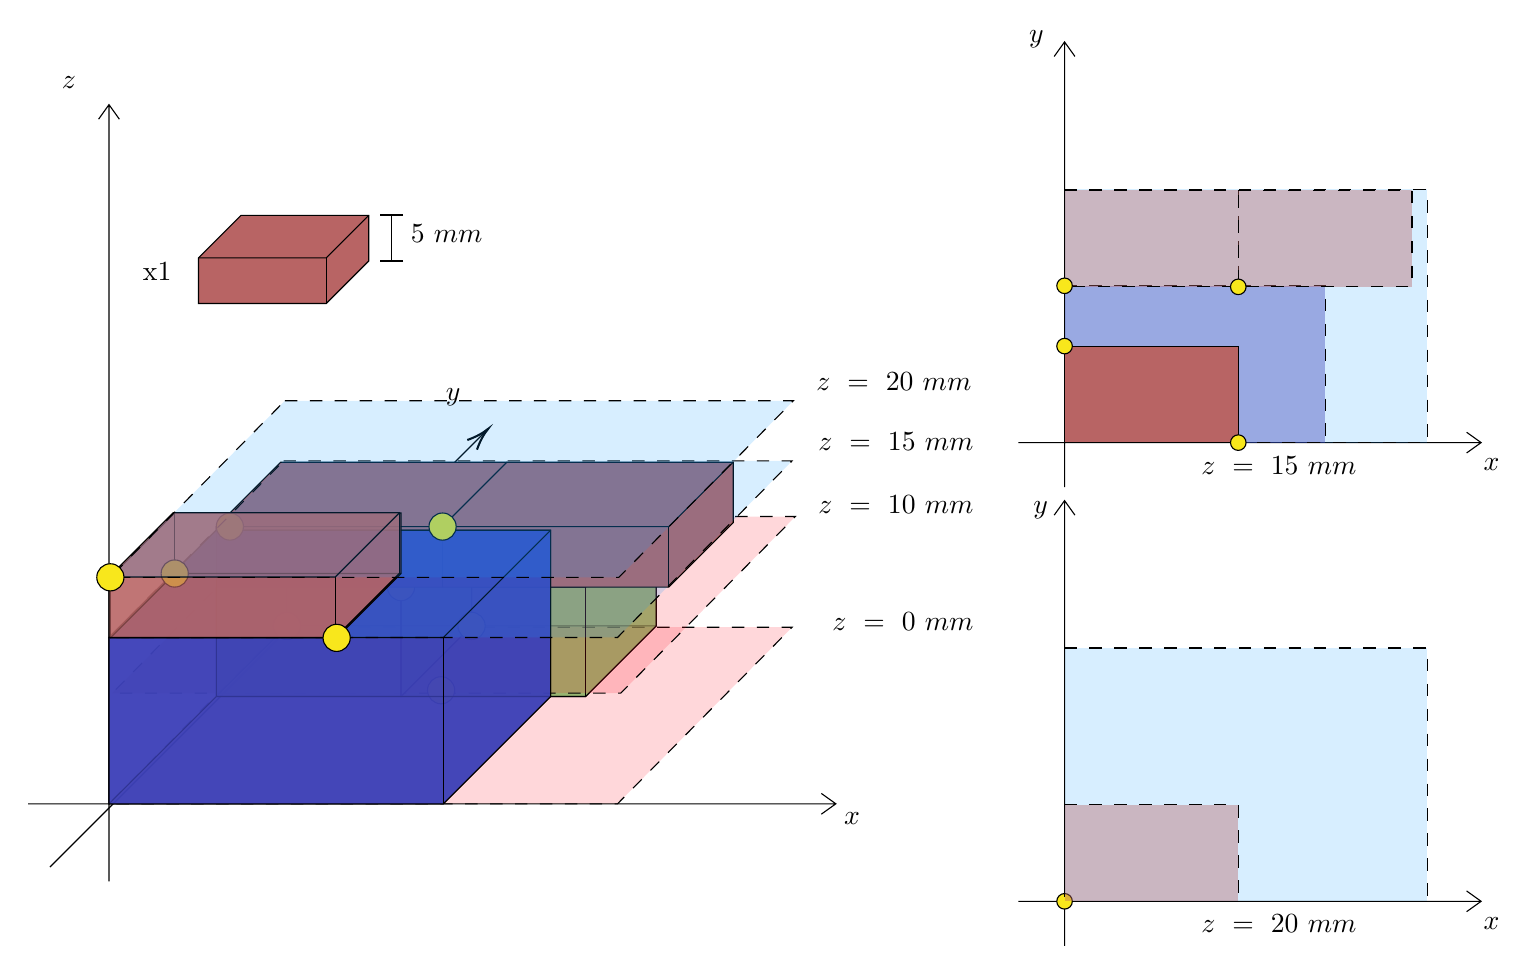
\begin{tikzpicture}[x=0.75pt,y=0.75pt,yscale=-1,xscale=1]
%uncomment if require: \path (0,511); %set diagram left start at 0, and has height of 511

%Shape: Cube [id:dp13382747579819188] 
\draw  [fill={rgb, 255:red, 130; green, 184; blue, 100 }  ,fill opacity=0.63 ] (400.59,311.37) -- (366.58,345.38) -- (277.6,345.38) -- (277.6,292.66) -- (311.6,258.65) -- (400.59,258.65) -- cycle ; \draw   (277.6,345.38) -- (311.6,311.37) -- (400.59,311.37) ; \draw   (311.6,311.37) -- (311.6,258.65) ;
%Shape: Parallelogram [id:dp6966422926494509] 
\draw  [fill={rgb, 255:red, 255; green, 17; blue, 34 }  ,fill opacity=0.17 ][dash pattern={on 4.5pt off 4.5pt}] (221,312) -- (466,312) -- (381.91,397.07) -- (136.91,397.07) -- cycle ;
%Shape: Cube [id:dp7954856505993868] 
\draw  [fill={rgb, 255:red, 130; green, 184; blue, 100 }  ,fill opacity=0.63 ] (277.6,292.66) -- (311.6,258.65) -- (400.59,258.65) -- (400.59,311.37) -- (366.58,345.38) -- (277.6,345.38) -- cycle ; \draw   (400.59,258.65) -- (366.58,292.66) -- (277.6,292.66) ; \draw   (366.58,292.66) -- (366.58,345.38) ;
%Shape: Parallelogram [id:dp4537315333431484] 
\draw  [fill={rgb, 255:red, 255; green, 17; blue, 34 }  ,fill opacity=0.17 ][dash pattern={on 4.5pt off 4.5pt}] (222.62,258.65) -- (467.62,258.65) -- (383.53,343.73) -- (138.53,343.73) -- cycle ;
%Shape: Axis 2D [id:dp9498145046786112] 
\draw  (98,397.07) -- (487.11,397.07)(136.91,60.22) -- (136.91,434.5) (480.11,392.07) -- (487.11,397.07) -- (480.11,402.07) (131.91,67.22) -- (136.91,60.22) -- (141.91,67.22)  ;
%Straight Lines [id:da4658635517686608] 
\draw    (108.47,427.52) -- (318.19,217.8) ;
\draw [shift={(319.6,216.39)}, rotate = 135] [color={rgb, 255:red, 0; green, 0; blue, 0 }  ][line width=0.75]    (10.93,-3.29) .. controls (6.95,-1.4) and (3.31,-0.3) .. (0,0) .. controls (3.31,0.3) and (6.95,1.4) .. (10.93,3.29)   ;
%Shape: Cube [id:dp037325029593255565] 
\draw  [fill={rgb, 255:red, 184; green, 100; blue, 100 }  ,fill opacity=1 ] (180.05,134.05) -- (200.55,113.55) -- (262.05,113.55) -- (262.05,135.55) -- (241.55,156.05) -- (180.05,156.05) -- cycle ; \draw   (262.05,113.55) -- (241.55,134.05) -- (180.05,134.05) ; \draw   (241.55,134.05) -- (241.55,156.05) ;
%Straight Lines [id:da907575610680141] 
\draw    (273.05,113.55) -- (273.05,135.55) ;
\draw [shift={(273.05,135.55)}, rotate = 270] [color={rgb, 255:red, 0; green, 0; blue, 0 }  ][line width=0.75]    (0,5.59) -- (0,-5.59)   ;
\draw [shift={(273.05,113.55)}, rotate = 270] [color={rgb, 255:red, 0; green, 0; blue, 0 }  ][line width=0.75]    (0,5.59) -- (0,-5.59)   ;
%Shape: Cube [id:dp07109550183608815] 
\draw  [fill={rgb, 255:red, 130; green, 184; blue, 100 }  ,fill opacity=0.63 ] (311.6,311.37) -- (277.6,345.38) -- (188.61,345.38) -- (188.61,292.66) -- (222.62,258.65) -- (311.6,258.65) -- cycle ; \draw   (188.61,345.38) -- (222.62,311.37) -- (311.6,311.37) ; \draw   (222.62,311.37) -- (222.62,258.65) ;
%Shape: Cube [id:dp004470545573486695] 
\draw  [fill={rgb, 255:red, 130; green, 184; blue, 100 }  ,fill opacity=0.63 ] (188.61,292.66) -- (222.62,258.65) -- (311.6,258.65) -- (311.6,311.37) -- (277.6,345.38) -- (188.61,345.38) -- cycle ; \draw   (311.6,258.65) -- (277.6,292.66) -- (188.61,292.66) ; \draw   (277.6,292.66) -- (277.6,345.38) ;
%Shape: Ellipse [id:dp6668747084579564] 
\draw  [fill={rgb, 255:red, 248; green, 231; blue, 28 }  ,fill opacity=1 ] (216.07,311.37) .. controls (216.07,307.75) and (219,304.82) .. (222.62,304.82) .. controls (226.23,304.82) and (229.16,307.75) .. (229.16,311.37) .. controls (229.16,314.98) and (226.23,317.91) .. (222.62,317.91) .. controls (219,317.91) and (216.07,314.98) .. (216.07,311.37) -- cycle ;
%Shape: Axis 2D [id:dp44476464107887725] 
\draw  (575,223.05) -- (798,223.05)(597.3,30) -- (597.3,244.5) (791,218.05) -- (798,223.05) -- (791,228.05) (592.3,37) -- (597.3,30) -- (602.3,37)  ;
%Shape: Rectangle [id:dp8842448402236128] 
\draw  [fill={rgb, 255:red, 17; green, 154; blue, 255 }  ,fill opacity=0.17 ][dash pattern={on 4.5pt off 4.5pt}] (597.3,101) -- (772,101) -- (772,223.05) -- (597.3,223.05) -- cycle ;
%Shape: Rectangle [id:dp22549871314391357] 
\draw  [fill={rgb, 255:red, 61; green, 65; blue, 184 }  ,fill opacity=0.4 ][dash pattern={on 4.5pt off 4.5pt}] (597.3,147.5) -- (723,147.5) -- (723,223.05) -- (597.3,223.05) -- cycle ;
%Shape: Ellipse [id:dp8550857930670437] 
\draw  [fill={rgb, 255:red, 248; green, 231; blue, 28 }  ,fill opacity=1 ] (305.06,311.37) .. controls (305.06,307.75) and (307.99,304.82) .. (311.6,304.82) .. controls (315.22,304.82) and (318.15,307.75) .. (318.15,311.37) .. controls (318.15,314.98) and (315.22,317.91) .. (311.6,317.91) .. controls (307.99,317.91) and (305.06,314.98) .. (305.06,311.37) -- cycle ;
%Shape: Ellipse [id:dp09363312581695205] 
\draw  [fill={rgb, 255:red, 248; green, 231; blue, 28 }  ,fill opacity=1 ] (271.05,292.66) .. controls (271.05,289.05) and (273.98,286.12) .. (277.6,286.12) .. controls (281.21,286.12) and (284.14,289.05) .. (284.14,292.66) .. controls (284.14,296.28) and (281.21,299.21) .. (277.6,299.21) .. controls (273.98,299.21) and (271.05,296.28) .. (271.05,292.66) -- cycle ;
%Shape: Ellipse [id:dp7691678960010918] 
\draw  [fill={rgb, 255:red, 248; green, 231; blue, 28 }  ,fill opacity=1 ] (290.37,342.37) .. controls (290.37,338.76) and (293.3,335.83) .. (296.91,335.83) .. controls (300.52,335.83) and (303.45,338.76) .. (303.45,342.37) .. controls (303.45,345.98) and (300.52,348.91) .. (296.91,348.91) .. controls (293.3,348.91) and (290.37,345.98) .. (290.37,342.37) -- cycle ;
%Shape: Cube [id:dp0837514121075894] 
\draw  [fill={rgb, 255:red, 184; green, 100; blue, 100 }  ,fill opacity=1 ] (188.61,263.5) -- (219.61,232.5) -- (328.63,232.5) -- (328.63,261.66) -- (297.63,292.66) -- (188.61,292.66) -- cycle ; \draw   (328.63,232.5) -- (297.63,263.5) -- (188.61,263.5) ; \draw   (297.63,263.5) -- (297.63,292.66) ;
%Shape: Cube [id:dp22596641921194294] 
\draw  [fill={rgb, 255:red, 184; green, 100; blue, 100 }  ,fill opacity=1 ] (297.63,263.5) -- (328.63,232.5) -- (437.65,232.5) -- (437.65,261.66) -- (406.65,292.66) -- (297.63,292.66) -- cycle ; \draw   (437.65,232.5) -- (406.65,263.5) -- (297.63,263.5) ; \draw   (406.65,263.5) -- (406.65,292.66) ;
%Shape: Cube [id:dp9390528785176023] 
\draw  [fill={rgb, 255:red, 61; green, 65; blue, 184 }  ,fill opacity=0.8 ] (349.7,345.38) -- (298,397.07) -- (136.91,397.07) -- (136.91,316.94) -- (188.61,265.25) -- (349.7,265.25) -- cycle ; \draw   (136.91,397.07) -- (188.61,345.38) -- (349.7,345.38) ; \draw   (188.61,345.38) -- (188.61,265.25) ;
%Shape: Cube [id:dp4332809548010883] 
\draw  [fill={rgb, 255:red, 61; green, 65; blue, 184 }  ,fill opacity=0.8 ] (136.91,316.94) -- (188.61,265.25) -- (349.7,265.25) -- (349.7,345.38) -- (298,397.07) -- (136.91,397.07) -- cycle ; \draw   (349.7,265.25) -- (298,316.94) -- (136.91,316.94) ; \draw   (298,316.94) -- (298,397.07) ;
%Shape: Ellipse [id:dp8530820745955504] 
\draw  [fill={rgb, 255:red, 248; green, 231; blue, 28 }  ,fill opacity=1 ] (188.61,263.5) .. controls (188.61,259.89) and (191.54,256.96) .. (195.15,256.96) .. controls (198.77,256.96) and (201.69,259.89) .. (201.69,263.5) .. controls (201.69,267.11) and (198.77,270.04) .. (195.15,270.04) .. controls (191.54,270.04) and (188.61,267.11) .. (188.61,263.5) -- cycle ;
%Shape: Ellipse [id:dp7570025851179228] 
\draw  [fill={rgb, 255:red, 248; green, 231; blue, 28 }  ,fill opacity=1 ] (291.09,263.5) .. controls (291.09,259.89) and (294.02,256.96) .. (297.63,256.96) .. controls (301.24,256.96) and (304.17,259.89) .. (304.17,263.5) .. controls (304.17,267.11) and (301.24,270.04) .. (297.63,270.04) .. controls (294.02,270.04) and (291.09,267.11) .. (291.09,263.5) -- cycle ;
%Shape: Parallelogram [id:dp8088836688018484] 
\draw  [fill={rgb, 255:red, 17; green, 154; blue, 255 }  ,fill opacity=0.17 ][dash pattern={on 4.5pt off 4.5pt}] (221,231.87) -- (466,231.87) -- (381.91,316.94) -- (136.91,316.94) -- cycle ;
%Shape: Rectangle [id:dp8807699745453305] 
\draw  [fill={rgb, 255:red, 184; green, 100; blue, 100 }  ,fill opacity=0.4 ][dash pattern={on 4.5pt off 4.5pt}] (597.3,101.5) -- (681,101.5) -- (681,148) -- (597.3,148) -- cycle ;
%Shape: Rectangle [id:dp7105108279475557] 
\draw  [fill={rgb, 255:red, 184; green, 100; blue, 100 }  ,fill opacity=0.4 ][dash pattern={on 4.5pt off 4.5pt}] (681,101.5) -- (764.7,101.5) -- (764.7,148) -- (681,148) -- cycle ;
%Shape: Circle [id:dp7943424960137139] 
\draw  [fill={rgb, 255:red, 248; green, 231; blue, 28 }  ,fill opacity=1 ] (593.55,147.5) .. controls (593.55,145.43) and (595.23,143.75) .. (597.3,143.75) .. controls (599.37,143.75) and (601.05,145.43) .. (601.05,147.5) .. controls (601.05,149.57) and (599.37,151.25) .. (597.3,151.25) .. controls (595.23,151.25) and (593.55,149.57) .. (593.55,147.5) -- cycle ;
%Shape: Circle [id:dp9005405536776231] 
\draw  [fill={rgb, 255:red, 248; green, 231; blue, 28 }  ,fill opacity=1 ] (677.25,148) .. controls (677.25,145.93) and (678.93,144.25) .. (681,144.25) .. controls (683.07,144.25) and (684.75,145.93) .. (684.75,148) .. controls (684.75,150.07) and (683.07,151.75) .. (681,151.75) .. controls (678.93,151.75) and (677.25,150.07) .. (677.25,148) -- cycle ;
%Shape: Cube [id:dp653646926223087] 
\draw  [fill={rgb, 255:red, 184; green, 100; blue, 100 }  ,fill opacity=0.67 ] (277.6,286.12) -- (246.6,317.12) -- (137.57,317.12) -- (137.57,287.96) -- (168.57,256.96) -- (277.6,256.96) -- cycle ; \draw   (137.57,317.12) -- (168.57,286.12) -- (277.6,286.12) ; \draw   (168.57,286.12) -- (168.57,256.96) ;
%Shape: Ellipse [id:dp6705610706320286] 
\draw  [fill={rgb, 255:red, 248; green, 231; blue, 28 }  ,fill opacity=1 ] (162.03,286.12) .. controls (162.03,282.51) and (164.96,279.58) .. (168.57,279.58) .. controls (172.19,279.58) and (175.12,282.51) .. (175.12,286.12) .. controls (175.12,289.73) and (172.19,292.66) .. (168.57,292.66) .. controls (164.96,292.66) and (162.03,289.73) .. (162.03,286.12) -- cycle ;
%Shape: Cube [id:dp7235035205502207] 
\draw  [fill={rgb, 255:red, 184; green, 100; blue, 100 }  ,fill opacity=0.67 ] (136.91,287.78) -- (167.91,256.78) -- (276.93,256.78) -- (276.93,285.94) -- (245.93,316.94) -- (136.91,316.94) -- cycle ; \draw   (276.93,256.78) -- (245.93,287.78) -- (136.91,287.78) ; \draw   (245.93,287.78) -- (245.93,316.94) ;
%Shape: Ellipse [id:dp5459811026373071] 
\draw  [fill={rgb, 255:red, 248; green, 231; blue, 28 }  ,fill opacity=1 ] (240.05,317.12) .. controls (240.05,313.51) and (242.98,310.58) .. (246.6,310.58) .. controls (250.21,310.58) and (253.14,313.51) .. (253.14,317.12) .. controls (253.14,320.73) and (250.21,323.66) .. (246.6,323.66) .. controls (242.98,323.66) and (240.05,320.73) .. (240.05,317.12) -- cycle ;
%Shape: Parallelogram [id:dp6357278096082768] 
\draw  [fill={rgb, 255:red, 17; green, 154; blue, 255 }  ,fill opacity=0.17 ][dash pattern={on 4.5pt off 4.5pt}] (221.66,202.88) -- (466.66,202.88) -- (382.57,287.96) -- (137.57,287.96) -- cycle ;
%Shape: Ellipse [id:dp5454534055037792] 
\draw  [fill={rgb, 255:red, 248; green, 231; blue, 28 }  ,fill opacity=1 ] (131.03,287.96) .. controls (131.03,284.34) and (133.96,281.41) .. (137.57,281.41) .. controls (141.19,281.41) and (144.12,284.34) .. (144.12,287.96) .. controls (144.12,291.57) and (141.19,294.5) .. (137.57,294.5) .. controls (133.96,294.5) and (131.03,291.57) .. (131.03,287.96) -- cycle ;
%Shape: Axis 2D [id:dp13890777694672107] 
\draw  (575,444.05) -- (798,444.05)(597.3,251) -- (597.3,465.5) (791,439.05) -- (798,444.05) -- (791,449.05) (592.3,258) -- (597.3,251) -- (602.3,258)  ;
%Shape: Rectangle [id:dp5079067412188037] 
\draw  [fill={rgb, 255:red, 17; green, 154; blue, 255 }  ,fill opacity=0.17 ][dash pattern={on 4.5pt off 4.5pt}] (597.3,322) -- (772,322) -- (772,444.05) -- (597.3,444.05) -- cycle ;
%Shape: Circle [id:dp4515950519247576] 
\draw  [fill={rgb, 255:red, 248; green, 231; blue, 28 }  ,fill opacity=1 ] (593.55,444.05) .. controls (593.55,441.98) and (595.23,440.3) .. (597.3,440.3) .. controls (599.37,440.3) and (601.05,441.98) .. (601.05,444.05) .. controls (601.05,446.12) and (599.37,447.8) .. (597.3,447.8) .. controls (595.23,447.8) and (593.55,446.12) .. (593.55,444.05) -- cycle ;
%Shape: Rectangle [id:dp8775041721420133] 
\draw  [fill={rgb, 255:red, 184; green, 100; blue, 100 }  ,fill opacity=0.4 ][dash pattern={on 4.5pt off 4.5pt}] (597.3,397.55) -- (681,397.55) -- (681,444.05) -- (597.3,444.05) -- cycle ;
%Shape: Rectangle [id:dp19056688106305508] 
\draw  [fill={rgb, 255:red, 184; green, 100; blue, 100 }  ,fill opacity=1 ] (597.3,176.55) -- (681,176.55) -- (681,223.05) -- (597.3,223.05) -- cycle ;
%Shape: Circle [id:dp3722307923482907] 
\draw  [fill={rgb, 255:red, 248; green, 231; blue, 28 }  ,fill opacity=1 ] (593.55,176.55) .. controls (593.55,174.48) and (595.23,172.8) .. (597.3,172.8) .. controls (599.37,172.8) and (601.05,174.48) .. (601.05,176.55) .. controls (601.05,178.62) and (599.37,180.3) .. (597.3,180.3) .. controls (595.23,180.3) and (593.55,178.62) .. (593.55,176.55) -- cycle ;
%Shape: Circle [id:dp8906369239154822] 
\draw  [fill={rgb, 255:red, 248; green, 231; blue, 28 }  ,fill opacity=1 ] (677.25,223.05) .. controls (677.25,220.98) and (678.93,219.3) .. (681,219.3) .. controls (683.07,219.3) and (684.75,220.98) .. (684.75,223.05) .. controls (684.75,225.12) and (683.07,226.8) .. (681,226.8) .. controls (678.93,226.8) and (677.25,225.12) .. (677.25,223.05) -- cycle ;

% Text Node
\draw (484.19,303.66) node [anchor=north west][inner sep=0.75pt]    {$z\ =\ 0\ mm$};
% Text Node
\draw (297.9,195.7) node [anchor=north west][inner sep=0.75pt]    {$y$};
% Text Node
\draw (489.84,399.85) node [anchor=north west][inner sep=0.75pt]    {$x$};
% Text Node
\draw (112.94,45.64) node [anchor=north west][inner sep=0.75pt]    {$z$};
% Text Node
\draw (152,135) node [anchor=north west][inner sep=0.75pt]   [align=left] {x1};
% Text Node
\draw (281.05,116.95) node [anchor=north west][inner sep=0.75pt]    {$5\ mm$};
% Text Node
\draw (477.48,217.2) node [anchor=north west][inner sep=0.75pt]    {$z\ =\ 15\ mm$};
% Text Node
\draw (798,229.4) node [anchor=north west][inner sep=0.75pt]    {$x$};
% Text Node
\draw (662,228.4) node [anchor=north west][inner sep=0.75pt]    {$z\ =\ 15\ mm$};
% Text Node
\draw (477.48,247.2) node [anchor=north west][inner sep=0.75pt]    {$z\ =\ 10\ mm$};
% Text Node
\draw (476.48,188.2) node [anchor=north west][inner sep=0.75pt]    {$z\ =\ 20\ mm$};
% Text Node
\draw (798,450.4) node [anchor=north west][inner sep=0.75pt]    {$x$};
% Text Node
\draw (662,449.4) node [anchor=north west][inner sep=0.75pt]    {$z\ =\ 20\ mm$};
% Text Node
\draw (581,250.4) node [anchor=north west][inner sep=0.75pt]    {$y$};
% Text Node
\draw (579,23.4) node [anchor=north west][inner sep=0.75pt]    {$y$};


\end{tikzpicture}

            }
        \end{figure}
    \end{frame}
    \begin{frame}{Support Planes}
        \begin{figure}[h]
            \resizebox*{!}{65mm}{%
            

\tikzset{every picture/.style={line width=0.75pt}} %set default line width to 0.75pt        

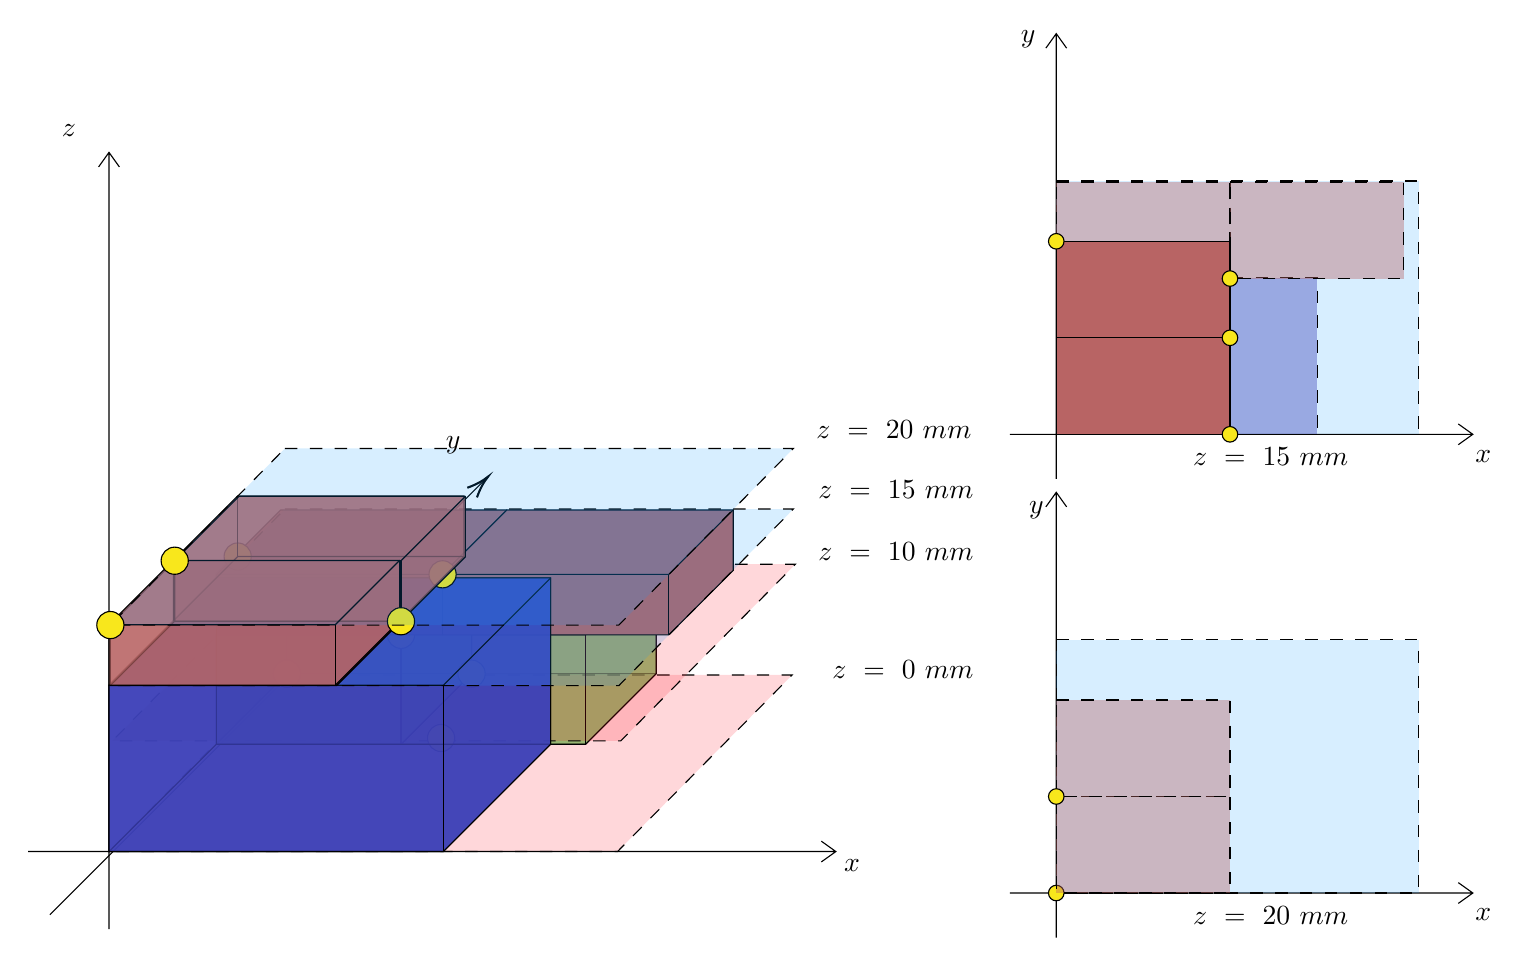
\begin{tikzpicture}[x=0.75pt,y=0.75pt,yscale=-1,xscale=1]
%uncomment if require: \path (0,517); %set diagram left start at 0, and has height of 517

%Shape: Cube [id:dp11750686891379902] 
\draw  [fill={rgb, 255:red, 130; green, 184; blue, 100 }  ,fill opacity=0.63 ] (420.59,331.37) -- (386.58,365.38) -- (297.6,365.38) -- (297.6,312.66) -- (331.6,278.65) -- (420.59,278.65) -- cycle ; \draw   (297.6,365.38) -- (331.6,331.37) -- (420.59,331.37) ; \draw   (331.6,331.37) -- (331.6,278.65) ;
%Shape: Parallelogram [id:dp761777526623073] 
\draw  [fill={rgb, 255:red, 255; green, 17; blue, 34 }  ,fill opacity=0.17 ][dash pattern={on 4.5pt off 4.5pt}] (241,332) -- (486,332) -- (401.91,417.07) -- (156.91,417.07) -- cycle ;
%Shape: Cube [id:dp9555955121552152] 
\draw  [fill={rgb, 255:red, 130; green, 184; blue, 100 }  ,fill opacity=0.63 ] (297.6,312.66) -- (331.6,278.65) -- (420.59,278.65) -- (420.59,331.37) -- (386.58,365.38) -- (297.6,365.38) -- cycle ; \draw   (420.59,278.65) -- (386.58,312.66) -- (297.6,312.66) ; \draw   (386.58,312.66) -- (386.58,365.38) ;
%Shape: Parallelogram [id:dp12159792926522017] 
\draw  [fill={rgb, 255:red, 255; green, 17; blue, 34 }  ,fill opacity=0.17 ][dash pattern={on 4.5pt off 4.5pt}] (242.62,278.65) -- (487.62,278.65) -- (403.53,363.73) -- (158.53,363.73) -- cycle ;
%Shape: Axis 2D [id:dp7547094969171453] 
\draw  (118,417.07) -- (507.11,417.07)(156.91,80.22) -- (156.91,454.5) (500.11,412.07) -- (507.11,417.07) -- (500.11,422.07) (151.91,87.22) -- (156.91,80.22) -- (161.91,87.22)  ;
%Straight Lines [id:da24486641728962577] 
\draw    (128.47,447.52) -- (338.19,237.8) ;
\draw [shift={(339.6,236.39)}, rotate = 135] [color={rgb, 255:red, 0; green, 0; blue, 0 }  ][line width=0.75]    (10.93,-3.29) .. controls (6.95,-1.4) and (3.31,-0.3) .. (0,0) .. controls (3.31,0.3) and (6.95,1.4) .. (10.93,3.29)   ;
%Shape: Cube [id:dp23740733074506637] 
\draw  [fill={rgb, 255:red, 130; green, 184; blue, 100 }  ,fill opacity=0.63 ] (331.6,331.37) -- (297.6,365.38) -- (208.61,365.38) -- (208.61,312.66) -- (242.62,278.65) -- (331.6,278.65) -- cycle ; \draw   (208.61,365.38) -- (242.62,331.37) -- (331.6,331.37) ; \draw   (242.62,331.37) -- (242.62,278.65) ;
%Shape: Cube [id:dp3377626309437859] 
\draw  [fill={rgb, 255:red, 130; green, 184; blue, 100 }  ,fill opacity=0.63 ] (208.61,312.66) -- (242.62,278.65) -- (331.6,278.65) -- (331.6,331.37) -- (297.6,365.38) -- (208.61,365.38) -- cycle ; \draw   (331.6,278.65) -- (297.6,312.66) -- (208.61,312.66) ; \draw   (297.6,312.66) -- (297.6,365.38) ;
%Shape: Ellipse [id:dp12890825920267357] 
\draw  [fill={rgb, 255:red, 248; green, 231; blue, 28 }  ,fill opacity=1 ] (236.07,331.37) .. controls (236.07,327.75) and (239,324.82) .. (242.62,324.82) .. controls (246.23,324.82) and (249.16,327.75) .. (249.16,331.37) .. controls (249.16,334.98) and (246.23,337.91) .. (242.62,337.91) .. controls (239,337.91) and (236.07,334.98) .. (236.07,331.37) -- cycle ;
%Shape: Axis 2D [id:dp22371680020517593] 
\draw  (591,216.05) -- (814,216.05)(613.3,23) -- (613.3,237.5) (807,211.05) -- (814,216.05) -- (807,221.05) (608.3,30) -- (613.3,23) -- (618.3,30)  ;
%Shape: Rectangle [id:dp19927589587496886] 
\draw  [fill={rgb, 255:red, 17; green, 154; blue, 255 }  ,fill opacity=0.17 ][dash pattern={on 4.5pt off 4.5pt}] (613.3,94) -- (788,94) -- (788,216.05) -- (613.3,216.05) -- cycle ;
%Shape: Rectangle [id:dp49701772163413693] 
\draw  [fill={rgb, 255:red, 61; green, 65; blue, 184 }  ,fill opacity=0.4 ][dash pattern={on 4.5pt off 4.5pt}] (613.3,140.5) -- (739,140.5) -- (739,216.05) -- (613.3,216.05) -- cycle ;
%Shape: Ellipse [id:dp9255158437533428] 
\draw  [fill={rgb, 255:red, 248; green, 231; blue, 28 }  ,fill opacity=1 ] (325.06,331.37) .. controls (325.06,327.75) and (327.99,324.82) .. (331.6,324.82) .. controls (335.22,324.82) and (338.15,327.75) .. (338.15,331.37) .. controls (338.15,334.98) and (335.22,337.91) .. (331.6,337.91) .. controls (327.99,337.91) and (325.06,334.98) .. (325.06,331.37) -- cycle ;
%Shape: Ellipse [id:dp7703154945024709] 
\draw  [fill={rgb, 255:red, 248; green, 231; blue, 28 }  ,fill opacity=1 ] (291.05,312.66) .. controls (291.05,309.05) and (293.98,306.12) .. (297.6,306.12) .. controls (301.21,306.12) and (304.14,309.05) .. (304.14,312.66) .. controls (304.14,316.28) and (301.21,319.21) .. (297.6,319.21) .. controls (293.98,319.21) and (291.05,316.28) .. (291.05,312.66) -- cycle ;
%Shape: Ellipse [id:dp2590138006968361] 
\draw  [fill={rgb, 255:red, 248; green, 231; blue, 28 }  ,fill opacity=1 ] (310.37,362.37) .. controls (310.37,358.76) and (313.3,355.83) .. (316.91,355.83) .. controls (320.52,355.83) and (323.45,358.76) .. (323.45,362.37) .. controls (323.45,365.98) and (320.52,368.91) .. (316.91,368.91) .. controls (313.3,368.91) and (310.37,365.98) .. (310.37,362.37) -- cycle ;
%Shape: Cube [id:dp2760918772938089] 
\draw  [fill={rgb, 255:red, 184; green, 100; blue, 100 }  ,fill opacity=1 ] (208.61,283.5) -- (239.61,252.5) -- (348.63,252.5) -- (348.63,281.66) -- (317.63,312.66) -- (208.61,312.66) -- cycle ; \draw   (348.63,252.5) -- (317.63,283.5) -- (208.61,283.5) ; \draw   (317.63,283.5) -- (317.63,312.66) ;
%Shape: Cube [id:dp25888946519283873] 
\draw  [fill={rgb, 255:red, 184; green, 100; blue, 100 }  ,fill opacity=1 ] (317.63,283.5) -- (348.63,252.5) -- (457.65,252.5) -- (457.65,281.66) -- (426.65,312.66) -- (317.63,312.66) -- cycle ; \draw   (457.65,252.5) -- (426.65,283.5) -- (317.63,283.5) ; \draw   (426.65,283.5) -- (426.65,312.66) ;
%Shape: Cube [id:dp5116746047827113] 
\draw  [fill={rgb, 255:red, 61; green, 65; blue, 184 }  ,fill opacity=0.8 ] (369.7,365.38) -- (318,417.07) -- (156.91,417.07) -- (156.91,336.94) -- (208.61,285.25) -- (369.7,285.25) -- cycle ; \draw   (156.91,417.07) -- (208.61,365.38) -- (369.7,365.38) ; \draw   (208.61,365.38) -- (208.61,285.25) ;
%Shape: Cube [id:dp9793419692541124] 
\draw  [fill={rgb, 255:red, 61; green, 65; blue, 184 }  ,fill opacity=0.8 ] (156.91,336.94) -- (208.61,285.25) -- (369.7,285.25) -- (369.7,365.38) -- (318,417.07) -- (156.91,417.07) -- cycle ; \draw   (369.7,285.25) -- (318,336.94) -- (156.91,336.94) ; \draw   (318,336.94) -- (318,417.07) ;
%Shape: Parallelogram [id:dp012772412734990968] 
\draw  [fill={rgb, 255:red, 17; green, 154; blue, 255 }  ,fill opacity=0.17 ][dash pattern={on 4.5pt off 4.5pt}] (241.66,252.05) -- (486.66,252.05) -- (402.57,337.12) -- (157.57,337.12) -- cycle ;
%Shape: Rectangle [id:dp19856633465195028] 
\draw  [fill={rgb, 255:red, 184; green, 100; blue, 100 }  ,fill opacity=0.4 ][dash pattern={on 4.5pt off 4.5pt}] (613.3,94.5) -- (697,94.5) -- (697,141) -- (613.3,141) -- cycle ;
%Shape: Rectangle [id:dp9568505376978227] 
\draw  [fill={rgb, 255:red, 184; green, 100; blue, 100 }  ,fill opacity=0.4 ][dash pattern={on 4.5pt off 4.5pt}] (697,94.5) -- (780.7,94.5) -- (780.7,141) -- (697,141) -- cycle ;
%Shape: Axis 2D [id:dp905993353659617] 
\draw  (591,437.05) -- (814,437.05)(613.3,244) -- (613.3,458.5) (807,432.05) -- (814,437.05) -- (807,442.05) (608.3,251) -- (613.3,244) -- (618.3,251)  ;
%Shape: Rectangle [id:dp7116456668997998] 
\draw  [fill={rgb, 255:red, 17; green, 154; blue, 255 }  ,fill opacity=0.17 ][dash pattern={on 4.5pt off 4.5pt}] (613.3,315) -- (788,315) -- (788,437.05) -- (613.3,437.05) -- cycle ;
%Shape: Circle [id:dp6552301353176846] 
\draw  [fill={rgb, 255:red, 248; green, 231; blue, 28 }  ,fill opacity=1 ] (609.55,437.05) .. controls (609.55,434.98) and (611.23,433.3) .. (613.3,433.3) .. controls (615.37,433.3) and (617.05,434.98) .. (617.05,437.05) .. controls (617.05,439.12) and (615.37,440.8) .. (613.3,440.8) .. controls (611.23,440.8) and (609.55,439.12) .. (609.55,437.05) -- cycle ;
%Shape: Rectangle [id:dp45682836776869995] 
\draw  [fill={rgb, 255:red, 184; green, 100; blue, 100 }  ,fill opacity=0.4 ][dash pattern={on 4.5pt off 4.5pt}] (613.3,390.55) -- (697,390.55) -- (697,437.05) -- (613.3,437.05) -- cycle ;
%Shape: Rectangle [id:dp057027447735892856] 
\draw  [fill={rgb, 255:red, 184; green, 100; blue, 100 }  ,fill opacity=1 ] (613.3,169.55) -- (697,169.55) -- (697,216.05) -- (613.3,216.05) -- cycle ;
%Shape: Circle [id:dp893710699889989] 
\draw  [fill={rgb, 255:red, 248; green, 231; blue, 28 }  ,fill opacity=1 ] (693.25,216.05) .. controls (693.25,213.98) and (694.93,212.3) .. (697,212.3) .. controls (699.07,212.3) and (700.75,213.98) .. (700.75,216.05) .. controls (700.75,218.12) and (699.07,219.8) .. (697,219.8) .. controls (694.93,219.8) and (693.25,218.12) .. (693.25,216.05) -- cycle ;
%Shape: Ellipse [id:dp6797422863626328] 
\draw  [fill={rgb, 255:red, 248; green, 231; blue, 28 }  ,fill opacity=1 ] (212.37,274.94) .. controls (212.37,271.33) and (215.3,268.4) .. (218.91,268.4) .. controls (222.52,268.4) and (225.45,271.33) .. (225.45,274.94) .. controls (225.45,278.56) and (222.52,281.49) .. (218.91,281.49) .. controls (215.3,281.49) and (212.37,278.56) .. (212.37,274.94) -- cycle ;
%Shape: Ellipse [id:dp1667953327037479] 
\draw  [fill={rgb, 255:red, 248; green, 231; blue, 28 }  ,fill opacity=1 ] (311.09,283.5) .. controls (311.09,279.89) and (314.02,276.96) .. (317.63,276.96) .. controls (321.24,276.96) and (324.17,279.89) .. (324.17,283.5) .. controls (324.17,287.11) and (321.24,290.04) .. (317.63,290.04) .. controls (314.02,290.04) and (311.09,287.11) .. (311.09,283.5) -- cycle ;
%Shape: Cube [id:dp8379525701182935] 
\draw  [fill={rgb, 255:red, 184; green, 100; blue, 100 }  ,fill opacity=0.67 ] (297.6,306.12) -- (266.6,337.12) -- (157.57,337.12) -- (157.57,307.96) -- (188.57,276.96) -- (297.6,276.96) -- cycle ; \draw   (157.57,337.12) -- (188.57,306.12) -- (297.6,306.12) ; \draw   (188.57,306.12) -- (188.57,276.96) ;
%Shape: Cube [id:dp526221096875487] 
\draw  [fill={rgb, 255:red, 184; green, 100; blue, 100 }  ,fill opacity=0.67 ] (327.93,274.94) -- (296.93,305.94) -- (187.91,305.94) -- (187.91,276.78) -- (218.91,245.78) -- (327.93,245.78) -- cycle ; \draw   (187.91,305.94) -- (218.91,274.94) -- (327.93,274.94) ; \draw   (218.91,274.94) -- (218.91,245.78) ;
%Shape: Cube [id:dp19903463769753094] 
\draw  [fill={rgb, 255:red, 184; green, 100; blue, 100 }  ,fill opacity=0.67 ] (188.57,276.96) -- (219.57,245.96) -- (328.6,245.96) -- (328.6,275.12) -- (297.6,306.12) -- (188.57,306.12) -- cycle ; \draw   (328.6,245.96) -- (297.6,276.96) -- (188.57,276.96) ; \draw   (297.6,276.96) -- (297.6,306.12) ;
%Shape: Cube [id:dp8602856031053141] 
\draw  [fill={rgb, 255:red, 184; green, 100; blue, 100 }  ,fill opacity=0.67 ] (156.91,307.78) -- (187.91,276.78) -- (296.93,276.78) -- (296.93,305.94) -- (265.93,336.94) -- (156.91,336.94) -- cycle ; \draw   (296.93,276.78) -- (265.93,307.78) -- (156.91,307.78) ; \draw   (265.93,307.78) -- (265.93,336.94) ;
%Shape: Ellipse [id:dp4815406681346305] 
\draw  [fill={rgb, 255:red, 248; green, 231; blue, 28 }  ,fill opacity=1 ] (291.05,306.12) .. controls (291.05,302.51) and (293.98,299.58) .. (297.6,299.58) .. controls (301.21,299.58) and (304.14,302.51) .. (304.14,306.12) .. controls (304.14,309.73) and (301.21,312.66) .. (297.6,312.66) .. controls (293.98,312.66) and (291.05,309.73) .. (291.05,306.12) -- cycle ;
%Shape: Parallelogram [id:dp8761855833958668] 
\draw  [fill={rgb, 255:red, 17; green, 154; blue, 255 }  ,fill opacity=0.17 ][dash pattern={on 4.5pt off 4.5pt}] (241.66,222.88) -- (486.66,222.88) -- (402.57,307.96) -- (157.57,307.96) -- cycle ;
%Shape: Ellipse [id:dp18311715249003535] 
\draw  [fill={rgb, 255:red, 248; green, 231; blue, 28 }  ,fill opacity=1 ] (151.03,307.96) .. controls (151.03,304.34) and (153.96,301.41) .. (157.57,301.41) .. controls (161.19,301.41) and (164.12,304.34) .. (164.12,307.96) .. controls (164.12,311.57) and (161.19,314.5) .. (157.57,314.5) .. controls (153.96,314.5) and (151.03,311.57) .. (151.03,307.96) -- cycle ;
%Shape: Ellipse [id:dp8613169128999868] 
\draw  [fill={rgb, 255:red, 248; green, 231; blue, 28 }  ,fill opacity=1 ] (182.03,276.96) .. controls (182.03,273.34) and (184.96,270.41) .. (188.57,270.41) .. controls (192.19,270.41) and (195.12,273.34) .. (195.12,276.96) .. controls (195.12,280.57) and (192.19,283.5) .. (188.57,283.5) .. controls (184.96,283.5) and (182.03,280.57) .. (182.03,276.96) -- cycle ;
%Shape: Rectangle [id:dp49121416555728614] 
\draw  [fill={rgb, 255:red, 184; green, 100; blue, 100 }  ,fill opacity=0.4 ][dash pattern={on 4.5pt off 4.5pt}] (613.3,344.05) -- (697,344.05) -- (697,390.55) -- (613.3,390.55) -- cycle ;
%Shape: Circle [id:dp8077543912869247] 
\draw  [fill={rgb, 255:red, 248; green, 231; blue, 28 }  ,fill opacity=1 ] (609.55,390.55) .. controls (609.55,388.48) and (611.23,386.8) .. (613.3,386.8) .. controls (615.37,386.8) and (617.05,388.48) .. (617.05,390.55) .. controls (617.05,392.62) and (615.37,394.3) .. (613.3,394.3) .. controls (611.23,394.3) and (609.55,392.62) .. (609.55,390.55) -- cycle ;
%Shape: Rectangle [id:dp4869036595737919] 
\draw  [fill={rgb, 255:red, 184; green, 100; blue, 100 }  ,fill opacity=1 ] (613.3,123.05) -- (697,123.05) -- (697,169.55) -- (613.3,169.55) -- cycle ;
%Shape: Circle [id:dp883887984988515] 
\draw  [fill={rgb, 255:red, 248; green, 231; blue, 28 }  ,fill opacity=1 ] (693.25,141) .. controls (693.25,138.93) and (694.93,137.25) .. (697,137.25) .. controls (699.07,137.25) and (700.75,138.93) .. (700.75,141) .. controls (700.75,143.07) and (699.07,144.75) .. (697,144.75) .. controls (694.93,144.75) and (693.25,143.07) .. (693.25,141) -- cycle ;
%Shape: Circle [id:dp6519707767315044] 
\draw  [fill={rgb, 255:red, 248; green, 231; blue, 28 }  ,fill opacity=1 ] (693.25,169.55) .. controls (693.25,167.48) and (694.93,165.8) .. (697,165.8) .. controls (699.07,165.8) and (700.75,167.48) .. (700.75,169.55) .. controls (700.75,171.62) and (699.07,173.3) .. (697,173.3) .. controls (694.93,173.3) and (693.25,171.62) .. (693.25,169.55) -- cycle ;
%Shape: Circle [id:dp6617436886058339] 
\draw  [fill={rgb, 255:red, 248; green, 231; blue, 28 }  ,fill opacity=1 ] (609.55,123.05) .. controls (609.55,120.98) and (611.23,119.3) .. (613.3,119.3) .. controls (615.37,119.3) and (617.05,120.98) .. (617.05,123.05) .. controls (617.05,125.12) and (615.37,126.8) .. (613.3,126.8) .. controls (611.23,126.8) and (609.55,125.12) .. (609.55,123.05) -- cycle ;

% Text Node
\draw (504.19,323.66) node [anchor=north west][inner sep=0.75pt]    {$z\ =\ 0\ mm$};
% Text Node
\draw (317.9,215.7) node [anchor=north west][inner sep=0.75pt]    {$y$};
% Text Node
\draw (509.84,419.85) node [anchor=north west][inner sep=0.75pt]    {$x$};
% Text Node
\draw (132.94,65.64) node [anchor=north west][inner sep=0.75pt]    {$z$};
% Text Node
\draw (497.48,237.2) node [anchor=north west][inner sep=0.75pt]    {$z\ =\ 15\ mm$};
% Text Node
\draw (814,222.4) node [anchor=north west][inner sep=0.75pt]    {$x$};
% Text Node
\draw (678,221.4) node [anchor=north west][inner sep=0.75pt]    {$z\ =\ 15\ mm$};
% Text Node
\draw (497.48,267.2) node [anchor=north west][inner sep=0.75pt]    {$z\ =\ 10\ mm$};
% Text Node
\draw (496.48,208.2) node [anchor=north west][inner sep=0.75pt]    {$z\ =\ 20\ mm$};
% Text Node
\draw (814,443.4) node [anchor=north west][inner sep=0.75pt]    {$x$};
% Text Node
\draw (678,442.4) node [anchor=north west][inner sep=0.75pt]    {$z\ =\ 20\ mm$};
% Text Node
\draw (595,20.4) node [anchor=north west][inner sep=0.75pt]    {$y$};
% Text Node
\draw (599,247.4) node [anchor=north west][inner sep=0.75pt]    {$y$};


\end{tikzpicture}

            }
        \end{figure}
    \end{frame}
    \begin{frame}{Support Planes}
        \begin{figure}[h]
            \resizebox*{!}{65mm}{%
            

\tikzset{every picture/.style={line width=0.75pt}} %set default line width to 0.75pt        

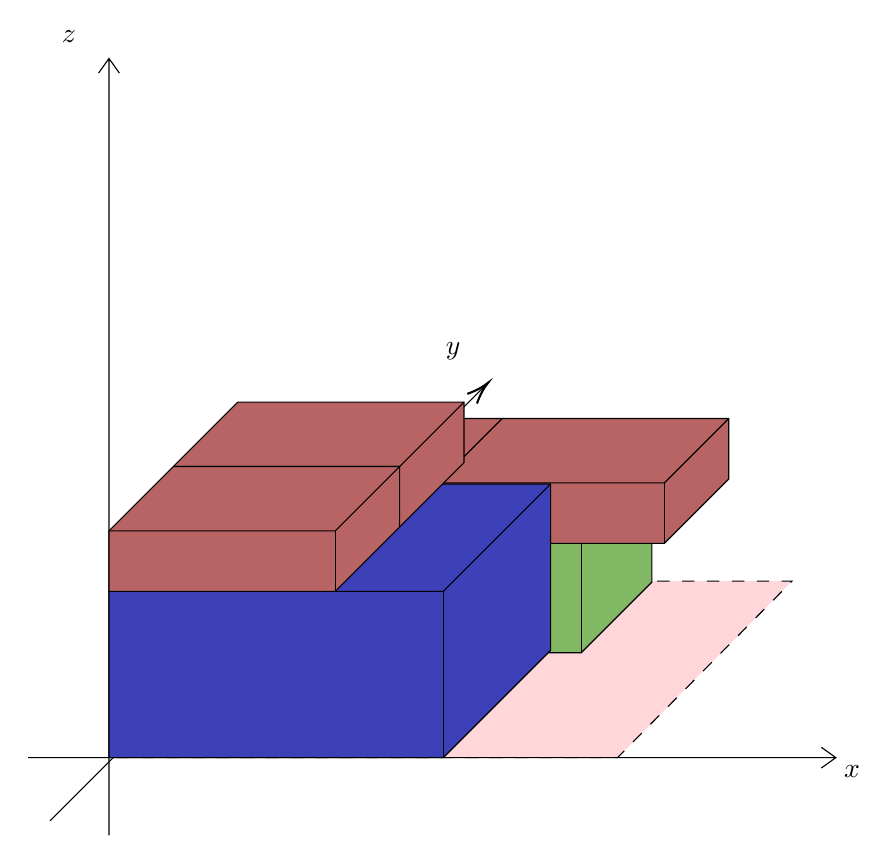
\begin{tikzpicture}[x=0.75pt,y=0.75pt,yscale=-1,xscale=1]
%uncomment if require: \path (0,441); %set diagram left start at 0, and has height of 441

%Shape: Parallelogram [id:dp6336164728589061] 
\draw  [fill={rgb, 255:red, 255; green, 17; blue, 34 }  ,fill opacity=0.17 ][dash pattern={on 4.5pt off 4.5pt}] (261,308.5) -- (506,308.5) -- (421.91,393.57) -- (176.91,393.57) -- cycle ;
%Shape: Axis 2D [id:dp545790083210709] 
\draw  (138,393.57) -- (527.11,393.57)(176.91,56.72) -- (176.91,431) (520.11,388.57) -- (527.11,393.57) -- (520.11,398.57) (171.91,63.72) -- (176.91,56.72) -- (181.91,63.72)  ;
%Straight Lines [id:da23076777818637972] 
\draw    (148.47,424.02) -- (358.19,214.3) ;
\draw [shift={(359.6,212.89)}, rotate = 135] [color={rgb, 255:red, 0; green, 0; blue, 0 }  ][line width=0.75]    (10.93,-3.29) .. controls (6.95,-1.4) and (3.31,-0.3) .. (0,0) .. controls (3.31,0.3) and (6.95,1.4) .. (10.93,3.29)   ;
%Shape: Cube [id:dp6994519250263277] 
\draw  [fill={rgb, 255:red, 130; green, 184; blue, 100 }  ,fill opacity=1 ] (226.47,290.32) -- (260.48,256.32) -- (349.46,256.32) -- (349.46,309.03) -- (315.46,343.04) -- (226.47,343.04) -- cycle ; \draw   (349.46,256.32) -- (315.46,290.32) -- (226.47,290.32) ; \draw   (315.46,290.32) -- (315.46,343.04) ;
%Shape: Cube [id:dp07364374934794116] 
\draw  [fill={rgb, 255:red, 130; green, 184; blue, 100 }  ,fill opacity=1 ] (315.46,290.32) -- (349.46,256.32) -- (438.45,256.32) -- (438.45,309.03) -- (404.44,343.04) -- (315.46,343.04) -- cycle ; \draw   (438.45,256.32) -- (404.44,290.32) -- (315.46,290.32) ; \draw   (404.44,290.32) -- (404.44,343.04) ;
%Shape: Cube [id:dp8273351088299524] 
\draw  [fill={rgb, 255:red, 184; green, 100; blue, 100 }  ,fill opacity=1 ] (226.47,261.16) -- (257.47,230.16) -- (366.49,230.16) -- (366.49,259.32) -- (335.49,290.32) -- (226.47,290.32) -- cycle ; \draw   (366.49,230.16) -- (335.49,261.16) -- (226.47,261.16) ; \draw   (335.49,261.16) -- (335.49,290.32) ;
%Shape: Cube [id:dp12028810160505032] 
\draw  [fill={rgb, 255:red, 184; green, 100; blue, 100 }  ,fill opacity=1 ] (335.49,261.16) -- (366.49,230.16) -- (475.51,230.16) -- (475.51,259.32) -- (444.51,290.32) -- (335.49,290.32) -- cycle ; \draw   (475.51,230.16) -- (444.51,261.16) -- (335.49,261.16) ; \draw   (444.51,261.16) -- (444.51,290.32) ;
%Shape: Cube [id:dp015004623257364513] 
\draw  [fill={rgb, 255:red, 61; green, 65; blue, 184 }  ,fill opacity=1 ] (176.91,313.44) -- (228.61,261.75) -- (389.7,261.75) -- (389.7,341.88) -- (338,393.57) -- (176.91,393.57) -- cycle ; \draw   (389.7,261.75) -- (338,313.44) -- (176.91,313.44) ; \draw   (338,313.44) -- (338,393.57) ;
%Shape: Cube [id:dp6659863306674686] 
\draw  [fill={rgb, 255:red, 184; green, 100; blue, 100 }  ,fill opacity=1 ] (207.91,253.28) -- (238.91,222.28) -- (347.93,222.28) -- (347.93,251.44) -- (316.93,282.44) -- (207.91,282.44) -- cycle ; \draw   (347.93,222.28) -- (316.93,253.28) -- (207.91,253.28) ; \draw   (316.93,253.28) -- (316.93,282.44) ;
%Shape: Cube [id:dp7671953057902039] 
\draw  [fill={rgb, 255:red, 184; green, 100; blue, 100 }  ,fill opacity=1 ] (176.91,284.28) -- (207.91,253.28) -- (316.93,253.28) -- (316.93,282.44) -- (285.93,313.44) -- (176.91,313.44) -- cycle ; \draw   (316.93,253.28) -- (285.93,284.28) -- (176.91,284.28) ; \draw   (285.93,284.28) -- (285.93,313.44) ;

% Text Node
\draw (337.9,192.2) node [anchor=north west][inner sep=0.75pt]    {$y$};
% Text Node
\draw (529.84,396.35) node [anchor=north west][inner sep=0.75pt]    {$x$};
% Text Node
\draw (152.94,42.14) node [anchor=north west][inner sep=0.75pt]    {$z$};


\end{tikzpicture}

            }
        \end{figure}
    \end{frame}

    \begin{frame}{Beam Search}
        \begin{itemize}
            \item Iteratively builds a solution
            \item Each node is a feasible packing
            \item Exploits support planes
            \item Different placement modes
            \item Explores $k$ best placements
        \end{itemize}
    \end{frame}
    \begin{frame}{Optimizations}
        \begin{columns}[onlytextwidth,T]
        \column{\dimexpr\linewidth-65mm-5mm}
            \begin{itemize}
                \item Duplicates removal
                \item Fast overlap checks
                \item Memory management
            \end{itemize}
        \column{65mm}
            \begin{figure}[h]
                \resizebox*{\columnwidth}{!}{%
                

\tikzset{every picture/.style={line width=0.75pt}} %set default line width to 0.75pt        

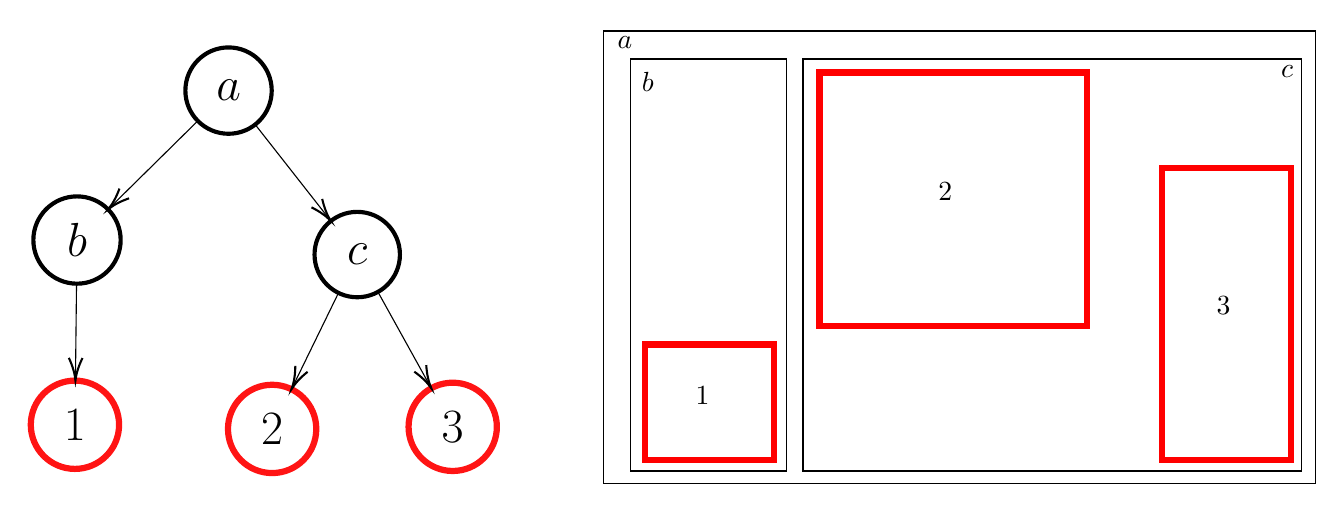
\begin{tikzpicture}[x=0.75pt,y=0.75pt,yscale=-1,xscale=1]
%uncomment if require: \path (0,269); %set diagram left start at 0, and has height of 269

%Shape: Rectangle [id:dp45712367712220003] 
\draw   (314,16.5) -- (657,16.5) -- (657,234.5) -- (314,234.5) -- cycle ;
%Shape: Rectangle [id:dp4249683313230568] 
\draw   (327,30) -- (402,30) -- (402,228.5) -- (327,228.5) -- cycle ;
%Shape: Rectangle [id:dp35105668268883494] 
\draw   (410,30) -- (650,30) -- (650,228.5) -- (410,228.5) -- cycle ;
%Shape: Rectangle [id:dp8308248735679132] 
\draw  [color={rgb, 255:red, 255; green, 0; blue, 0 }  ,draw opacity=1 ][line width=2.25]  (334,167.5) -- (396,167.5) -- (396,223) -- (334,223) -- cycle ;
%Shape: Rectangle [id:dp6177381470864712] 
\draw  [color={rgb, 255:red, 255; green, 0; blue, 0 }  ,draw opacity=1 ][line width=2.25]  (418,36.5) -- (547,36.5) -- (547,158.5) -- (418,158.5) -- cycle ;
%Shape: Rectangle [id:dp3774907556728889] 
\draw  [color={rgb, 255:red, 255; green, 0; blue, 0 }  ,draw opacity=1 ][line width=2.25]  (583,82.5) -- (645,82.5) -- (645,223) -- (583,223) -- cycle ;

% Text Node
\draw  [color={rgb, 255:red, 0; green, 0; blue, 0 }  ,draw opacity=1 ][line width=1.5]   (195.23, 124.2) circle [x radius= 20.57, y radius= 20.57]   ;
\draw (195.23,124.2) node  [font=\LARGE]  {$c$};
% Text Node
\draw  [color={rgb, 255:red, 0; green, 0; blue, 0 }  ,draw opacity=1 ][line width=1.5]   (60.22, 117.2) circle [x radius= 21.03, y radius= 21.03]   ;
\draw (60.22,117.2) node  [font=\LARGE]  {$b$};
% Text Node
\draw  [color={rgb, 255:red, 0; green, 0; blue, 0 }  ,draw opacity=1 ][line width=1.5]   (133.23, 45.2) circle [x radius= 20.8, y radius= 20.8]   ;
\draw (133.23,45.2) node  [font=\LARGE]  {$a$};
% Text Node
\draw  [color={rgb, 255:red, 255; green, 20; blue, 20 }  ,draw opacity=1 ][line width=2.25]   (59.22, 206.2) circle [x radius= 21.27, y radius= 21.27]   ;
\draw (59.22,206.2) node  [font=\LARGE]  {$1$};
% Text Node
\draw  [color={rgb, 255:red, 255; green, 20; blue, 20 }  ,draw opacity=1 ][line width=2.25]   (154.23, 208.2) circle [x radius= 21.27, y radius= 21.27]   ;
\draw (154.23,208.2) node  [font=\LARGE]  {$2$};
% Text Node
\draw  [color={rgb, 255:red, 255; green, 20; blue, 20 }  ,draw opacity=1 ][line width=2.25]   (241.23, 207.2) circle [x radius= 21.27, y radius= 21.27]   ;
\draw (241.23,207.2) node  [font=\LARGE]  {$3$};
% Text Node
\draw (324.23,22.2) node    {$a$};
% Text Node
\draw (335.23,41.2) node    {$b$};
% Text Node
\draw (643.23,36.2) node    {$c$};
% Text Node
\draw (357,186.4) node [anchor=north west][inner sep=0.75pt]    {$1$};
% Text Node
\draw (474,88.4) node [anchor=north west][inner sep=0.75pt]    {$2$};
% Text Node
\draw (608,143.4) node [anchor=north west][inner sep=0.75pt]    {$3$};
% Connection
\draw    (186.2,142.69) -- (164.44,187.28) ;
\draw [shift={(163.56,189.08)}, rotate = 296.02] [color={rgb, 255:red, 0; green, 0; blue, 0 }  ][line width=0.75]    (10.93,-3.29) .. controls (6.95,-1.4) and (3.31,-0.3) .. (0,0) .. controls (3.31,0.3) and (6.95,1.4) .. (10.93,3.29)   ;
% Connection
\draw    (205.2,142.2) -- (229.94,186.84) ;
\draw [shift={(230.91,188.59)}, rotate = 241] [color={rgb, 255:red, 0; green, 0; blue, 0 }  ][line width=0.75]    (10.93,-3.29) .. controls (6.95,-1.4) and (3.31,-0.3) .. (0,0) .. controls (3.31,0.3) and (6.95,1.4) .. (10.93,3.29)   ;
% Connection
\draw    (146.07,61.56) -- (181.29,106.44) ;
\draw [shift={(182.52,108.02)}, rotate = 231.87] [color={rgb, 255:red, 0; green, 0; blue, 0 }  ][line width=0.75]    (10.93,-3.29) .. controls (6.95,-1.4) and (3.31,-0.3) .. (0,0) .. controls (3.31,0.3) and (6.95,1.4) .. (10.93,3.29)   ;
% Connection
\draw    (118.42,59.8) -- (76.62,101.03) ;
\draw [shift={(75.2,102.43)}, rotate = 315.4] [color={rgb, 255:red, 0; green, 0; blue, 0 }  ][line width=0.75]    (10.93,-3.29) .. controls (6.95,-1.4) and (3.31,-0.3) .. (0,0) .. controls (3.31,0.3) and (6.95,1.4) .. (10.93,3.29)   ;
% Connection
\draw    (59.99,138.23) -- (59.49,182.93) ;
\draw [shift={(59.46,184.93)}, rotate = 270.64] [color={rgb, 255:red, 0; green, 0; blue, 0 }  ][line width=0.75]    (10.93,-3.29) .. controls (6.95,-1.4) and (3.31,-0.3) .. (0,0) .. controls (3.31,0.3) and (6.95,1.4) .. (10.93,3.29)   ;

\end{tikzpicture}

                }
                \caption{AABB Tree}
            \end{figure}
            %\vspace*{-15mm}
            %\begin{figure}
            %    \resizebox*{\columnwidth}{!}{%
            %    \begin{minipage}{\linewidth}
            %        \begin{align}
            %        hash_{ib} &= hash\_nc(b, x^s_i, y^s_i, z^s_i, w^s_i, d^s_i, h_i) \notag \\
            %        hash^s &= \sum\limits_{b \in B^s}{\sum\limits_{i \in J^s_b}{hash_{ib}}} \notag
            %        \end{align}
            %    \end{minipage}}
            %    \caption{Hash of a solution $s$}
            %\end{figure}
        \end{columns}
    \end{frame}

    \section{Conclusions}

    \begin{frame}{Computational Experiments}
        \begin{table}[htbp]
    \caption{Average execution time of literature results with bin gap}
    \centering
    \resizebox{\textwidth}{!}{\begin{tabular}{|l|l|c|c|c|c|c|}
    \hline
    \multicolumn{2}{|c|}{\textbf{Heuristic}} & \multicolumn{4}{|c|}{\textbf{Execution Time (s)}} & \textbf{Bin Gap (\%)} \\ \hline
    \multicolumn{2}{|c|}{} & $n=50$ & $n=100$ & $n=150$ & $n=200$ &  \\ \hline
    \textbf{PM} & $k=1$ & 0.03 & 0.11 & 0.28 & 0.54 & 5.82 \\ 
     & $k=5$ & 0.08 & 0.38 & 1.00 & 2.09 & 5.56 \\ 
     & $k=10$ & 0.15 & 0.73 & 1.93 & 4.00 & 5.54 \\ 
     & $k=20$ & 0.29 & 1.40 & 3.77 & 7.71 & 5.30 \\ 
     & $k=50$ & 0.70 & 3.50 & 9.39 & 19.59 & 5.19 \\ \hline
    \textbf{PS} & $k=1$ & 0.05 & 0.18 & 0.50 & 1.05 & 5.61 \\ 
     & $k=5$ & 0.12 & 0.72 & 2.10 & 4.62 & 5.26 \\ 
     & $k=10$ & 0.23 & 1.38 & 4.11 & 8.95 & 5.19 \\ 
     & $k=20$ & 0.46 & 2.67 & 8.21 & 17.64 & 4.98 \\ 
     & $k=50$ & 1.12 & 6.45 & 20.39 & 43.50 & 4.75 \\ \hline
     \hline
     \multicolumn{2}{|l|}{\textbf{BRKGA-VD}} & 17.13 & 80.63 & 190.50 & 369.75 & 0.00 \\ \hline
    \end{tabular}}
    \label{exp:literature_time_gap}
\end{table}
    
    \end{frame}

    \begin{frame}{Computational Experiments}
        \begin{table}[htbp]
    \centering
    \caption{Summary of case study tests}
    \resizebox{\columnwidth}{!}{\begin{tabular}{|c|c|c|c|c|c|c|}
    \hline
    & \multicolumn{ 3}{c|}{\textbf{PS}} & \multicolumn{ 3}{c|}{\textbf{PM}} \\ \hline
    \textbf{$k$} & \textbf{\textit{TT (ms)}} & \textbf{\textit{B}} & \textbf{\textit{CR (\%)}} & \textbf{\textit{TT (ms)}} & \textbf{\textit{B}} & \textbf{\textit{CR (\%)}} \\ \hline
    $1$ & 423.87 & 1.37 & 65.87 & 65.18 & 1.31 & \textbf{70.70} \\ 
    $5$ & 1,597.54 & 1.34 & 69.19 & 185.22 & 1.29 & \textbf{73.08} \\ 
    $10$ & 2,627.52 & 1.32 & 70.35 & 344.90 & 1.27 & \textbf{73.56} \\ 
    $20$ & 5,373.79 & 1.34 & 70.78 & 620.95 & 1.27 & \textbf{74.57} \\ 
    $50$ & 14,203.10 & 1.31 & 72.11 & 1,279.96 & 1.29 & \textbf{74.61} \\ 
    $100$ & 26,934.21 & 1.31 & 73.23 & 2,340.37 & 1.26 & \textbf{75.36} \\ 
    $200$ & 48,944.90 & 1.30 & 73.89 & 4,465.78 & 1.25 & \textbf{76.39} \\ \hline
    \end{tabular}}
    \label{results:usecase_summary}
    \end{table}
    
    \end{frame}

    \begin{frame}{Computational Experiments}
        \begin{table}[htbp]
    \caption{Case study experiments trade off between average execution times and average cage ratio}
    \centering
    \resizebox{\columnwidth}{!}{\begin{tabular}{|c|c|c|c|c|}
    \hline
    \multicolumn{1}{|c|}{\textbf{$k$}} & \multicolumn{ 2}{c|}{\textbf{\textit{PS}}} & \multicolumn{ 2}{c|}{\textbf{\textit{PM}}} \\ \hline
    \multicolumn{1}{|c|}{} & $\textbf{\textit{CR}} - \textbf{\textit{CR*}}$ \textbf{\textit{(\%)}} & $\textbf{\textit{TT}} - \textbf{\textit{TT* (ms)}}$ & $\textbf{\textit{CR}} - \textbf{\textit{CR*}}$ \textbf{\textit{(\%)}} & $\textbf{\textit{TT}} - \textbf{\textit{TT* (ms)}}$ \\ \hline
    1 & 10.56 & 358.69 & 5.73 & 0.00 \\
    5 & 7.24 & 1,532.36 & 3.35 & 120.04 \\
    10 & 6.08 & 2,562.34 & 2.87 & 279.72 \\
    \textbf{20} & 5.65 & 5,308.61 & \textbf{1.85} & \textbf{555.77} \\
    \textbf{50} & 4.32 & 14,137.92 & \textbf{1.82} & \textbf{1,214.78} \\
    100 & 3.20 & 26,869.03 & 1.07 & 2,275.19 \\
    200 & 2.54 & 48,879.72 & 0.04 & 4,400.60 \\ \hline
    \end{tabular}~}
    \label{exp:usecase_tradeoff}
\end{table}
    
    \end{frame}

    \begin{frame}{Results \& Future Developments}
    \end{frame}
\end{document}